%% Thesis 1.0
%% "Main Program"
%% 5/10/96 Rich Townsend

%% This is the main program which affects the overall
%% layout of the thesis, and patches all of the
%% chapters together

%% Set up the document class (hacked report)
%% One sided
%\documentclass[11pt, a4paper, oneside, openright, fleqn]{thesis}
%% Two sided
\documentclass[11pt, a4paper, twoside, openright, fleqn]{thesis}

%%%%%%%%%%%%%%%%%%%%%%%%%%%%%%%%%%%%%%%%%%%%%%%%%%%%%%%%%%
%% Package loading stuff
%%%%%%%%%%%%%%%%%%%%%%%%%%%%%%%%%%%%%%%%%%%%%%%%%%%%%%%%%%

% Load in srcltx package for xdvi link
%\usepackage{srcltx}
% NEEDS TO BE REMOVED BEFORE PRINTING!!!!
\usepackage[inactive]{srcltx}

\usepackage[dvipsnames]{color}

% Load in UCL logo package
%\usepackage{uclogo}

% Load in url package
\usepackage{url}

% Load in the xspace package
\usepackage{xspace}

% For adding footnotes to tables
\usepackage{threeparttable}

% For adding colour to tables
\usepackage{colortbl}

% For adding colour to tables
\usepackage[table]{xcolor}

% Load in the ifpdf package
\usepackage{ifpdf}

% Load in the epsf packages
\usepackage{enumerate}

% Load in subcaption package
\usepackage{subcaption} 

% Load in the epsf packages
\usepackage{epsf}

% Load in the epsfig packages
\usepackage{epsfig}

% Load in the calc package
\usepackage{calc}

% Load in Landscape package
\usepackage{lscape}

% Load in Longtable package
\usepackage{longtable}

% Load in Setspace package
\usepackage{setspace}

% Load in the Supertabular package
\usepackage{supertabular}

% Load in the Tabularx package
\usepackage{tabularx}

% Load in the Multirow package
\usepackage{multirow}

% Load in Curves package
\usepackage{curves}

% Load in Epic package
\usepackage{epic}

% Load in the rotating package
\usepackage{rotating}

% Load in the FancyHeadings package
\usepackage{fancyheadings}

% Load in the Afterpage package
\usepackage{afterpage}

% Load in the ifthen package
\usepackage{ifthen}

% Load in the harvard bib style package, and configure it
%\usepackage[abbr]{harvard}
%\citationstyle{apsr}
%\renewcommand{\harvardand}{\&}
%\newcommand{\natexlab}[1]{#1}

% Load in the AmsTeX packages
\usepackage{amsmath}
\usepackage{amssymb}

% Load in the caption
\usepackage{caption}

%ANTONIA PACKAGES
\usepackage{booktabs}


% Load in the hacked caption stuff
\usepackage{hackcaption}

% Load in PDF hyper link package
\usepackage{hyperref}

% % PDF hyperlinks, with coloured links 
% % (watch for {\it ...} usage - swap to \textit{...})
% \usepackage[pdftex,bookmarks,colorlinks,breaklinks,backref]{hyperref}
% \hypersetup{linkcolor=red,citecolor=blue} % coloured links
% %\hypersetup{linkcolor=black,citecolor=black} % black links, for printed output

% Load in Natbib package
\usepackage{natbib}
\newcommand{\harvardand}{\&}
% Defining the citation style of a given bib style:
% Use \bibpunct (in the preamble only) with 6 mandatory arguments:
%    1. opening bracket for citation
%    2. closing bracket
%    3. citation separator (for multiple citations in one \cite)
%    4. the letter n for numerical styles, s for superscripts
%        else anything for author-year
%    5. punctuation between authors and date
%    6. punctuation between years (or numbers) when common authors missing
% One optional argument is the character coming before post-notes. It
%   appears in square braces before all other arguments. May be left off.
% Example (and default) \bibpunct[, ]{(}{)}{;}{a}{,}{,}
\bibpunct[ ]{(}{)}{;}{a}{}{,}


%%%%%%%%%%%%%%%%%%%%%%%%%%%%%%%%%%%%%%%%%%%%%%%%%%%%%%%%%%
% Page style stuff
%%%%%%%%%%%%%%%%%%%%%%%%%%%%%%%%%%%%%%%%%%%%%%%%%%%%%%%%%%

% Set up the text width and margins in terms of the binding and outer
% margin lengths - here assigned the values dictated by UCL regulations
\newlength{\bindingmargin}
\newlength{\outermargin}
\setlength{\bindingmargin}{40mm}
\setlength{\outermargin}{20mm}


% Work out the text width from these margins and the page size
\setlength{\textwidth}{\paperwidth-\outermargin-\bindingmargin}


% Now work out the LaTeX oddside and evenside margins, taking into
% account the automatic 1in offset which is included.
\setlength{\oddsidemargin}{\bindingmargin-1in}
\setlength{\evensidemargin}{\paperwidth-\textwidth-\bindingmargin-1in}


% Set up all of the other page style stuff
\setlength{\textheight}{235mm}
\setlength{\topmargin}{-0.25in}            
\setlength{\headheight}{7mm}           
\setlength{\headsep}{8mm}              
\setlength{\footnotesep}{1.5ex}
\setlength{\textfloatsep}{14pt plus 6pt minus 2pt}
\renewcommand{\baselinestretch}{1.5}

%% F SIDOLI 2009-05-11
%% Standard empty clear page
\newcommand{\clearemptydoublepage}{\newpage\thispagestyle{empty}\cleardoublepage}
%% Redefined empty clear page to include blank page comment
\newcommand{\clearthesisemptydoublepage}
{\newpage\thispagestyle{headings}\clearthesisdoublepage}

\pagestyle{headings}
%% To add my personal footer to each page comment out line above
%% and uncomment the line below
%\pagestyle{thesis}

\newcommand{\longpage}{\enlargethispage{\baselineskip}}
\newcommand{\shortpage}{\enlargethispage{-\baselineskip}}
\newcommand{\longpagef}{\enlargethispage*{\baselineskip}}
\newcommand{\shortpagef}{\enlargethispage*{-\baselineskip}}
\newcommand{\rb}[1]{\raisebox{1.6ex}[0pt]{#1}}
%%%%%%%%%%%%%%%%%%%%%%%%%%%%%%%%%%%%%%%%%%%%%%%%%%%%%%%%%%

% Font diddles

% Map in the missing math times fonts (this prevents a warning -
% it doesn't do anything useful! )

\DeclareFontFamily{OMS}{ptm}{}
\DeclareFontShape{OMS}{ptm}{m}{n}{ <-> sub * cmsy/m/n }{}

%%%%%%%%%%%%%%%%%%%%%%%%%%%%%%%%%%%%%%%%%%%%%%%%%%%%%%%%%%

% Load in the defs
\typeout{Loading defs....}
%additional commands
\newcommand{\micron}{$\mu$m}
\newcommand{\halpha}{H$\alpha$}
\newcommand{\oilong}{[O~{\sc i}]~6300,6363~\AA}
\newcommand{\oishort}{[O~{\sc i}]}

% Commands to do the journal names for bibtex

\newcommand{\mnras}{MNRAS}
\newcommand{\apj}{ApJ}
\newcommand{\apjs}{ApJSS}
\newcommand{\apjl}{ApJL}
\newcommand{\aap}{A\&A}
\newcommand{\aaps}{A\&AS}
\newcommand{\apss}{Ap\&SS}
\newcommand{\pasp}{PASP}
\newcommand{\acta}{Act Ast}
\newcommand{\aj}{AJ}
\newcommand{\araa}{Ann. Rev. Astr. Astrophys.}
\newcommand{\baas}{BAAS}
\newcommand{\nat}{Nature}
\newcommand{\gca}{Geochimica et Cosmochimica Acta}
%%%%%%%%%%%%%%%%%%%%%%%%%%%%%%%%%%%%%%%%
\newcommand{\ndash}{\textendash}

%% Definitions for writing out ions, e.g., CIV [OIII]
%
\newcommand\eline[3]{\ensuremath{{\rm #1}\,{\textsc{#2}}{#3}}} 
\newcommand\fline[3]{\ensuremath{{[\rm #1}\,{\textsc{#2}]}{#3}}} 


% Stellar lines
\newcommand\Caii[1]{\eline{Ca}{ii}{#1}}
\newcommand\Cii[1]{\eline{C}{ii}{#1}}
\newcommand\Ciii[1]{\eline{C}{iii}{#1}}
\newcommand\Civ[1]{\eline{C}{iv}{#1}}
\newcommand\Ni[1]{\eline{N}{i}{#1}}
\newcommand\Nii[1]{\eline{N}{ii}{#1}}
\newcommand\Niii[1]{\eline{N}{iii}{#1}}
\newcommand\Niv[1]{\eline{N}{iv}{#1}}
\newcommand\Nv[1]{\eline{N}{v}{#1}}
\newcommand\Oi[1]{\eline{O}{i}{#1}}
\newcommand\Oii[1]{\eline{O}{ii}{#1}}
\newcommand\Oiv[1]{\eline{O}{iv}{#1}}
\newcommand\Ov[1]{\eline{O}{v}{#1}}
\newcommand\Ovi[1]{\eline{O}{vi}{#1}}
\newcommand\Ovii[1]{\eline{O}{vii}{#1}}
\newcommand\Oviii[1]{\eline{O}{viii}{#1}}
\newcommand\Silii[1]{\eline{Si}{ii}{#1}}
\newcommand\Siliii[1]{\eline{Si}{iii}{#1}}
\newcommand\Siliv[1]{\eline{Si}{iv}{#1}}
\newcommand\Feiv[1]{\eline{Fe}{iv}{#1}}
\newcommand\Feix[1]{\eline{Fe}{ix}{#1}}
\newcommand\Fexvii[1]{\eline{Fe}{xvii}{#1}}
\newcommand\Siii[1]{\eline{S}{iii}{#1}}


% Nebular lines
\newcommand\Hi[1]{\eline{H}{i}{#1}}
\newcommand\Hii[1]{\eline{H}{ii}{#1}}
\newcommand\Hei[1]{\eline{He}{i}{#1}}
\newcommand\Heii[1]{\eline{He}{ii}{#1}}
\newcommand\Bra{Br\ensuremath{\alpha}}
\newcommand\Brg{Br\ensuremath{\gamma}}
\newcommand{\ha}{H\ensuremath{\alpha}}
\newcommand{\hb}{H\ensuremath{\beta}}
\newcommand{\hg}{H\ensuremath{\gamma}}
\newcommand{\hd}{H\ensuremath{\delta}}
\newcommand\nebNi[1]{\fline{N}{i}{#1}}
\newcommand\nebNii[1]{\fline{N}{ii}{#1}}
\newcommand\nebNiii[1]{\fline{N}{iii}{#1}}
\newcommand\nebOi[1]{\fline{O}{i}{#1}}
\newcommand\nebOii[1]{\fline{O}{ii}{#1}}
\newcommand\nebOiii[1]{\fline{O}{iii}{#1}}
\newcommand\nebSi[1]{\fline{S}{i}{#1}}
\newcommand\nebSii[1]{\fline{S}{ii}{#1}}
\newcommand\nebSiii[1]{\fline{S}{iii}{#1}}
\newcommand\nebFeii[1]{\fline{Fe}{ii}{#1}}
\newcommand\nebFeiii[1]{\fline{Fe}{iii}{#1}}
\newcommand\nebFeiv[1]{\fline{Fe}{iv}{#1}}
\newcommand\nebAriii[1]{\fline{Ar}{iii}{#1}}
\newcommand\nebAriv[1]{\fline{Ar}{iv}{#1}}
\newcommand\nebCliii[1]{\fline{Cl}{iii}{#1}}
\newcommand\nebCliv[1]{\fline{Cl}{iv}{#1}}
\newcommand\nebNeiii[1]{\fline{Ne}{iii}{#1}}



%%%%%%%%%%%%%%%%%%%%%%%%%%%%%%%%%%%%%%%%

%% Definitions for writing variables in the form: X(Y)
\newcommand\var[2]{\ensuremath{#1({\rm #2})}}
\newcommand\varit[2]{\ensuremath{#1({#2})}}
\newcommand\varnp[2]{\ensuremath{#1{\rm #2}}} % no parentheses

% Shorthand forms
\newcommand\lum[1]{\var{L}{#1}}
\newcommand\ew[1]{\var{W}{#1}}
\newcommand\ewnp[1]{\varnp{W}{#1}}
\newcommand\intflux[1]{\var{I}{#1}} 
\newcommand\obsflux[1]{\var{F}{#1}} 
\newcommand\numb[1]{\var{N}{#1}}
\newcommand\chb{\var{c}{\hb}}
\newcommand\flam{\var{f}{\lambda}}
\newcommand\fhb{\var{f}{\hb}}
%%%%%%%%%%%%%%%%%%%%%%%%%%%%%%%%%%%%%%%%

%% Definitions for writing variables in the form:  X$_{y}^{z}$
\newcommand\ion[2]{\ensuremath{{\rm #1}^{\rm #2}}\xspace}
\newcommand\rscript[3]{\ensuremath{{#1}_{\rm #2}^{\rm #3}}}
\newcommand\lscript[3]{\ensuremath{^{\rm #1}_{\rm #2}{\rm #3}}}

%----- strong line ratio 
\newcommand\slratio[4]{\ensuremath{{#1}_{#2}{#3}_{#4}}\xspace}

 
% shorthand forms
\newcommand\qvalue[1]{\rscript{Q}{0}{#1}}
\newcommand\qone[1]{\rscript{Q}{1}{#1}}
\newcommand\qtwo[1]{\rscript{Q}{2}{#1}}
\newcommand\sigsfr{\rscript{\Sigma}{\rm SFR}{}}
\newcommand\etaz{\rscript{\eta}{0}{}}
\newcommand\etazt{\rscript{\eta}{0}{}(t)}
\newcommand\lsun{\rscript{L}{\odot}{}}
\newcommand\msun{\rscript{M}{\odot}{}}
\newcommand\vsun{\rscript{V}{\odot}{}}
\newcommand\zsun{\rscript{Z}{\odot}{}}
\newcommand\Te{\rscript{T}{e}{}}
\newcommand\Ne{\rscript{n}{e}{}}
\newcommand\Teff{\rscript{T}{eff}{}}
\newcommand\Reff{\rscript{R}{eff}{}}
%%%%%%%%%%%%%%%%%%%%%%%%%%%%%%%%%%%%%%%%

% Definitions for coordinate stuff
\newcommand{\h}{\ensuremath{^{\rm{h}}}}
\newcommand{\m}{\ensuremath{^{\rm{m}}}}
\newcommand{\s}{\ensuremath{^{\rm{s}}}}
\newcommand{\fdg}{\mbox{\ensuremath{.\!\!^\circ}}}    
\newcommand{\farcm}{\mbox{\ensuremath{.\mkern-4mu^\prime}}}   
\newcommand{\farcs}{\mbox{\ensuremath{.\!\!^{\prime\prime}}}}  
\newcommand{\fh}{\mbox{\ensuremath{.\!\!^{\rm{h}}}}}
\newcommand{\fm}{\mbox{\ensuremath{.\!\!^{\rm{m}}}}}
\newcommand{\fs}{\mbox{\ensuremath{.\!\!^{\rm{s}}}}}
\newcommand{\degr}{\ensuremath{^{\circ}}}
\newcommand{\arcsec}{\mbox{\ensuremath{^{\prime\prime}}}}
\newcommand\ra[4]{{#1}\h{#2}\m{#3}\fs{#4}}
\newcommand\dec[4]{{#1}\h{#2}\m{#3}\fs{#4}}
%%%%%%%%%%%%%%%%%%%%%%%%%%%%%%%%%%%%%%%%

% randoms

\newcommand{\eg}{{\rm e.g.,}}
\newcommand{\ie}{{\rm i.e.,}}
\newcommand{\etc}{{\rm etc}}
\newcommand{\cf}{{\rm cf.}}

%%%%%%%%%%%%%%%%%%%%%%%%%%%%%%%%%%%%%%%%

% multicolumn and multirow
\newcommand\mr[1]{\multirow{#1}{*}}
\newcommand\mcc[1]{\multicolumn{#1}{c}}
\newcommand\mcl[1]{\multicolumn{#1}{l}}
\newcommand\mcr[1]{\multicolumn{#1}{r}}

\newcommand{\df}{\dotfill}

%%%%%%%%%%%%%%%%%%%%%%%%%%%%%%%%%%%%%%%%

% sun symbols and units
\newcommand{\mz}{\ensuremath{\dot{M}-Z}}
\newcommand\kpc{\ensuremath{\rm kpc}}
\newcommand\mpc{\ensuremath{\rm Mpc}}
\newcommand\invmpc{\rscript{\rm Mpc}{}{-1}}
\newcommand\kms{\rscript{\rm km\,s}{}{-1}}
\newcommand\cmq{\rscript{\rm cm}{}{-3}}
\newcommand\ergss{\rscript{\rm ergs\,s}{}{-1}}
\newcommand\ergsscm{\rscript{\rm ergs\,s}{}{-1}\rscript{\rm cm}{}{-2}}
\newcommand\ergsscma{\rscript{\rm ergs\,s}{}{-1}\rscript{\rm cm}{}{-2}%
\rscript{\rm {\AA}}{}{-1}}
\newcommand\msunyr{\ensuremath{\msun\,{\rm yr^{-1}}}}
\newcommand\msunyrkpc{\ensuremath{\msunyr\,{\rm kpc^{-2}}}}
\newcommand\sq[1]{\rscript{#1}{}{2}}
%\newcommand\ebv[1][]{\ensuremath{{\rm E}(B-V)_{#1}}}
\newcommand\ebv[1]{\ensuremath{{\rm E}_{\textsc{b-v}}^{#1}}}
\newcommand\ebvg{\ebv{\rm Gal}}
\newcommand\ebvt{\ebv{\rm tot}}
\newcommand\ebvi{\ebv{\rm int}}
\newcommand\lam[1]{\ensuremath{\lambda\,{#1}}}
\newcommand\lamlam[1]{\ensuremath{\lambda\,\lambda\,{#1}}}
\newcommand{\mdot}{\ensuremath{\dot{M}}}
\newcommand\arith[3]{\ensuremath{#1\,#2\,#3}} 
\newcommand\ho{\arith{\rscript{H}{0}{}}{=}{75}{\kms\invmpc}}

\newcommand\caseA{Case $A$}
\newcommand\caseB{Case $B$}
\newcommand\caseC{Case $C$}

% Citation Aliases
% Examples
%  \citetalias{key}   ==>> text
%  \citepalias{key}   ==>> (text)
%
\defcitealias{leitherer99}{Baltimore}
\defcitealias{snc02}{UCL}
\defcitealias{meynet94}{Geneva}
\defcitealias{girardi00}{Padova}
\defcitealias{pauldrach01}{Pauldrach}
\defcitealias{hillier98}{Hillier}
\defcitealias{norris03}{Richard Norris}
\defcitealias{l.p.martins05}{Lucimara}
\defcitealias{lejeune97}{Lejeune}
\defcitealias{schmutz92}{Schmutz}

% Misc

\def\Starburst99{Starburst99}
\newcommand\ttfsc[1]{\textsc{\ttfamily #1}}
\def\mag{mag}
\newcommand\privcomm[2]{({#1,}{~priv. comm. #2})}
\newcommand\privcommnb[2]{{#1,}{~priv. comm. #2}} % nb = no brackets


% Telescope/instrument abbreviations

\def\hst{\textit{HST}}
\def\spitzer{\textit{Spitzer}}


% See if there are any includeonlys
%\typein[\inclist]{Enter includeonly...}
%\ifthenelse{\equal{}{\inclist}}{}{\includeonly{\inclist}}


%%%%%%%%%%%%%%%%%%%%%%%%%%%%%%%%%%%%%%%%%%%%%%%%%%%%%%%%%%%
% Document Start
%%%%%%%%%%%%%%%%%%%%%%%%%%%%%%%%%%%%%%%%%%%%%%%%%%%%%%%%%%%

% If you want to compile one chapter at a time
% but keep the numbering sorted. Must appear 
% before '\begin{document}'

% \includeonly{chapters/chapter1/chapter1}

%%%

\begin{document}

%%---------------------------------------------------------
%% Frontmatter
%%---------------------------------------------------------

%% Do the title page: Personal info for title page
\university{\huge University College London}
\faculty{\Large Faculty of Mathematics and Physical Sciences}
\department{Department of Physics \& Astronomy}  

\thesistitle{\vspace{1cm} Core-collapse supernova \\ dust masses from \\ line profile models}
\thesisauthor{\LARGE ANTONIA BEVAN \vspace{1cm}}
%\dedication{\it{DEDICATION}} 
\supervisorone{Prof. Michael J. Barlow}
\examinerone{Dr Kenneth Wood}
\supervisortwo{Dr Jeremy A. Yates}
\examinertwo{Prof. Ian D. Howarth}

\maketitle 


%% Declaration - REQUIRES SIGNING
\thispagestyle{empty}

\vspace*{3cm}

\begin{flushleft}
I, Antonia Bevan, confirm that the work presented in this thesis is my own. Where
information has been derived from other sources, I confirm that this has been indicated in
the thesis.
\end{flushleft}
%\clearemptydoublepage

%% Abstract
\thispagestyle{empty}
\begin{raggedleft}
\vspace*{23mm}
\hfill {\huge {\bf {Abstract}}} \\
\vspace{6mm}
\hfill \rule{4in}{.015in} \\
\vspace{19mm}
\end{raggedleft}

\noindent{Galaxies and quasars in the very early universe harbour considerable masses of dust, the source of which has been much contested.  For many years it was thought that core-collapse supernovae, though known to form small masses of dust via analyses of dust emission in the infra-red, could not account for the large quantities of dust seen in the early universe.  In recent years, however, this opinion has been challenged by the discovery of reservoirs of cool dust in a number of supernovae containing as much as 1M$_{\odot}$ of dust.  
The late time optical and near-IR line profiles of many core-collapse supernovae exhibit a red-blue asymmetry as a result of greater extinction by internal dust of radiation emitted from the receding parts of the supernova ejecta.  In this thesis, I present  a new code, {\sc damocles}, that models the effects of dust on the line profiles of core-collapse supernovae in order to determine the masses of newly formed dust that form in the ejecta.  The Monte Carlo code and the physical processes therein are described in detail and the testing of the code is presented.  Theoretical profiles are produced in order to understand the effects of varying the parameters of interest on the shapes of the modelled line profiles produced and I discuss a number of other signatures of dust extinction on line profiles aside from the expected blue-shifting.
{\sc damocles} was used to model four different supernovae and supernova remnants.  SN~1987A is a crucial object in the study of core--collapse supernovae and I first present a detailed investigation into the rate of dust formation in this object by modelling the evolution of the H$\alpha$ and [O~{\sc i}]$\lambda\lambda$6300,6363~\AA\ lines.  I also present models of the hydrogen and oxygen lines at late times from SN~1980K, SN~1993J and Cassiopeia A,  all of which display strong blue-shifted asymmetries.
I find that large dust masses are required to fit the late-time line profiles of all of these objects and conclude that core-collapse supernovae are likely an important source of dust in the universe.}





%% Acknowledgements
\thispagestyle{empty}
\begin{raggedleft}
\vspace*{23mm}
\hfill {\huge {\bf {Acknowledgements}}} \\
\vspace{6mm}
\hfill \rule{4in}{.015in} \\
\vspace{19mm}
\end{raggedleft}


\noindent{There are so many people that I want to thank -- you all, I hope, know who you are. But the last three years have been eventful and the writing of this thesis has been one of the lesser challenges.  
%Anyone reading this will probably understand what it means when I say that the writing of this thesis has been among the lesser challenges that I have faced during my PhD.  
And so, there are just a few, very heartfelt and uncharacteristically emotional, thanks that I wish to make.}
%\bigskip
%\noindent 
First and foremost, to Mike;  you have been endlessly patient and have always been generous with your time and advice.  You gave me the freedom and space to find my own path through my PhD, particularly in difficult times, and I am exceptionally grateful for this.  
%You have gone above and beyond, especially in difficult times, and I truly thank you.
To Jeremy; %your support over the last three years has been invaluable. ]
you advised me thoughtfully and carefully. Thanks for always having those encouraging words at the right moments.
%  your encouragement always seemed to come at the right times.  
To Patrick; %simply put, this thesis would not exist without you!  
thank you for everything -- %for advice on science and on life, for gossipy drinks and endless cups of tea, for giggling from the start to the end, for your patient understanding and for tea gin. 
from science advice to gossip to tea gin, this thesis probably wouldn't exist without you!
%\bigskip 
%\noindent 
To 
Benedict,
Dom,
Fiona,
Georgia,
George,
Jack,
and
Mike;  my luck in counting you as my friends is beyond words. %I know that every one of you would be there if I needed you, and 
Thank you all for being there on so many occasions, happy and sad.
% proved this on numerous occasions over the last three years.  
My life is so much the better for having the conversation, laughter and wisdom that you all bring to it.  
%\clearpage
%\bigskip
%\noindent 
To Alex;  you really did a good job growing up these last few years.  I could not be prouder to call you my brother.  Knowing that you are always there for me means more to me than you know. 
%\bigskip
%
%\noindent 
To Nick; you have been there for me in my darkest moments and my best.  
I cannot imagine having done this without you, and I have so many memories that I will cherish for the rest of my life.  
You got me through this 
%, as you get me through so much of my life.  
and you brightened every day. I am so grateful.
%\bigskip
%\noindent 
To Mum and Dad;  you have been, are, and will always be my best friends in the world.  Support does not even begin to cover what you have given me, not just over the last three years but my whole life.  You are both caring, generous and wise, and I am so lucky to be able to call you Mum and Dad.  Thank you.   




%%%%%%%%%%%%%%%%%%%%%%%%%%%%%%%%%%%%%%%%%%%%%%%%%%%%%%%%%%%%%%%%%%%%%%%%%%%
% If you have more than one page in your acknowledgements, include the
% following on each page after the first:
%
% \thispagestyle{fancyplain}
% \lhead[\fancyplain{}{\vspace{4mm}\thepage \vspace{0mm}}]{}
% \rhead[]{\fancyplain{}{\vspace{4mm}\thepage \vspace{0mm}}}
% \cfoot{}
%
%%%%%%%%%%%%%%%%%%%%%%%%%%%%%%%%%%%%%%%%%%%%%%%%%%%%%%%%%%%%%%%%%%%%%%%%%%%



%% Front quote
\thispagestyle{empty}
\vspace*{\fill}

\begin{flushright}
\large {\em Gather out of star-dust 

Earth-dust,

Cloud-dust,

Storm-dust,

And splinters of hail,

One handful of dream-dust

Not for sale.}\\

\ \

\normalsize

{- Langston Hughes}  

{\em Dream Dust}

% Oh God of dust and rainbows, help us see. That without dust the rainbow would not be - Langston Hughes
\end{flushright}


\vspace*{\fill}
\vspace*{\fill}


\vspace*{\fill}

\vspace*{\fill}

\vspace*{\fill}


%\clearemptydoublepage


%% Contents pages
\addcontentsline{toc}{chapter}{Table of Contents}
\tableofcontents
\clearthesisemptydoublepage
\addcontentsline{toc}{chapter}{List of Figures}
\listoffigures
\addcontentsline{toc}{chapter}{List of Tables}
\listoftables

\addcontentsline{toc}{chapter}{List of Acronyms}


%%List Of Acronyms
\thispagestyle{empty}
\begin{raggedleft}
\vspace*{23mm}
\hfill {\huge {\bf {List of Acronyms}}} \\
\vspace{6mm}
\hfill \rule{4in}{.015in} \\
\vspace{19mm}
\end{raggedleft}


AAT - Anglo-Australian Telescope

%%%%%%%%%%%%%%%%%%%%%%%%%%%%%%%%%%%%%%%%%%%%%%%%%%%%%%%%%%%%%%%%%%%%%%%%%%%
% If you have more than one page in your acknowledgements, include the
% following on each page after the first:
%
% \thispagestyle{fancyplain}
% \lhead[\fancyplain{}{\vspace{4mm}\thepage \vspace{0mm}}]{}
% \rhead[]{\fancyplain{}{\vspace{4mm}\thepage \vspace{0mm}}}
% \cfoot{}
%
%%%%%%%%%%%%%%%%%%%%%%%%%%%%%%%%%%%%%%%%%%%%%%%%%%%%%%%%%%%%%%%%%%%%%%%%%%%



CTIO - Cerro Tololo Inter-American Observatory

HST - Hubble Space Telescope

VLT - Very Large Telescope

%%---------------------------------------------------------
%% Main Body
%%---------------------------------------------------------

% Put your chapters in here


\chapter{Introduction}\label{chp:chp1}

%\begin{flushright}
%  {\em QUOTE GOES HERE }\\
%
%\ \
%
%\normalsize
%{AUTHOR}  
%\end{flushright}


\noindent{Should you choose to seek out one of my friends and ask them about my whereabouts in recent months,
%acquaintances and to enquire of them my whereabouts in recent months
 they would likely stare at you blankly.  Upon further interrogation they would probably yield the information that I was preoccupied writing about dust, a fact which I imagine they  find bemusing and possibly somewhat concerning.  Blissful as they are in their ignorance of dust (astronomers find no such peace), they do not know the importance of this all-pervading substance.}

The universe is an extremely dusty place.  The ubiquity of dust throughout almost all epochs and environments demands a comprehensive understanding of its formation and evolution, properties and effects.  It plays numerous roles in a variety of scenes; it is a building block of  all solid bodies, a birthing place for molecules, a crucial ingredient in star formation and an extreme annoyance for cosmologists.  It is both a product of physical processes and an agent of chemical ones.

It is perhaps confusing therefore that there is comparatively little consensus regarding the formation processes and natal environments that result in the evolution of certain atoms and molecules into the grains we call dust.  Over the years since the first discovery  of dust in the very early universe, a growing population of astronomers and astrophysicists have turned their attention to the study of dust formation in core-collapse supernovae (CCSNe), in the hope that these objects might prove to be the missing piece of the puzzle.  Recent observations of a number of core-collapse supernovae  and remnants have lent weight to this theory, with models and analyses of spectral energy distributions (SEDs)  suggesting the presence of large reservoirs of cool, ejecta-condensed dust. 

I have sought to make my own small contribution to this field by exploiting a different observational signature, that of  blue-shifted line profile asymmetries observed in the spectra of many CCSNe and attributed to the formation of dust in the ejecta.  By quantitatively modelling characteristically asymmetric spectral line profiles using a novel code, DAMOCLES, I have attempted to determine the rate of dust formation in CCSNe and the expected order of magnitude of the eventual dust masses produced.

Throughout the remainder of this chapter I will attempt to elucidate the above synopsis in more detail.  A brief discussion of the roles that dust plays in the universe will be followed by a summary of our current understanding of dust formation in CCSNe.  I will conclude this chapter with a short justification of the approach that I have adopted for this work and an outline of the structure of this thesis.


\section{A Handful of Dust}


\subsection{A Brief History}

The presence of dust in the universe was first theorised when astronomers observed dark patches of sky in the Milky Way where all of the stars had been ``erased" (see Figure \ref{intro:fig:dustpatch}).  Whilst some claimed that these black regions were in fact a true absence of stars resulting from some anomaly in the stellar distribution, others felt that it was more likely that an obscuring cloud of material was blocking the light from the stars behind.  In 1930, Donald \citeauthor{Trumpler1930} confirmed this latter theory by considering the apparent magnitudes and colours of stars located at different angles to the galactic plane, discovering that those closer to the plane appeared redder than their more distant counterparts.  This was the first evidence of interstellar reddening and the beginnings of our understanding of dust as a scatterer, absorber and emitter of radiation.

For the next few decades, dust was thought to be largely an irritating obstacle to observing and comprehending more interesting facets of the universe.  We now have a much fuller understanding of the variety and importance of the roles that dust plays throughout astrophysics.

\begin{figure}
\centering
\includegraphics[scale=0.8]{chapters/chapter1/figs/black_patch_B68.jpg}
\caption{The dark globule Barnard 68, LDN 57.  ESO press release 30 April 1999.}
\label{intro:fig:dustpatch}
\end{figure}

\subsection{The Roles of Dust in the Universe}

Despite comprising only $\sim$1\% of the mass of the interstellar medium (ISM), dust grains account for as much as 30\% of the total galactic luminosity via their emission in the infra-red (IR) \citep{Li2003}.  In the cycle of matter from the ISM to condensing clouds to stars and back again, dust is far more than a passive passenger along for the ride.  Whilst residing in the ISM, dust is important in determining its thermodynamics.  It acts both as a heating agent via the emission of photoelectrons in regions of strong ultra-violet (UV) radiation and a coolant in dense regions via the emission of IR radiation.  In this role as a coolant, dust is also crucial to the process of star-formation, helping to remove gravitational energy and allowing the natal cloud to collapse.  Dust also contributes to the star formation process by shielding the gas from ionising radiation, helping to speed up the construction of the protostellar core. 

In addition to the above physical functions, dust plays an essential part in chemical processes.  Heavy elements in the local medium are depleted through their inclusion in dust grains.  These grains  attract gaseous atoms to their surfaces and catalyse the formation of molecules which are then released back into the surrounding medium.

Dust does not reside solely in the ISM however.  It is present in  large quantities in the circumnuclear tori found around active galactic nuclei.  Dust is also found between planets, around stars and in protoplanetary discs, where dust grains are often the smallest unit of the building blocks that will go on to form planetesimals and planets.  These grains may even be responsible for the origins of life.  

The more detailed our understanding of dust as an astrophysical community, the more accurate we can make our inferences across an entire range of  fields.  There is arguably no other topic in astronomy that has such wide-ranging effects.


\subsection{The Medium of Dust}

An increasingly detailed knowledge of the nature and properties of dust has developed over the last few decades. Dust grains have their terrestrial analogue in soot or very fine sand rather than in the dust bunnies that one may find behind the sofa.  When found in the ISM they are generally small, between 0.05\micron\ and 0.25\micron\ in radius, and are normally predominantly composed of carbon or silicates.  Carbonaceous grains may take many forms ranging from structured solids such as diamond and graphite to amorphous molecules and aromatics.  They are generally found to be strongly attentuating.  Silicates tend to be more glassy and contain silicon and oxygen potentially with the dirtying addition of magnesium, iron or other heavier elements.  Condensates of more complex molecules such as olivine (MgFeSiO$_4$) and pyroxene (MgSiO$_3$) make up these grains.  

Whilst an increasingly strong picture of the composition and properties of dust is becoming apparent, there are still a number of largely unresolved issues regarding the makeup of a dusty medium.
Different species and composites thereof have different optical properties.  In order to model the absorption and scattering of radiation off dust grains it is necessary to first know the complex refractive indices of a given species over the relevant wavelength range.  Laboratory measurements have produced a number of different sets of optical constants for a variety of carbonaceous and silicate species and these are well-utilised throughout the field.  It is noted at this early juncture however that in many cases there are numerous, somewhat contradictory, sets of optical constants for a given species and that these variations can potentially cause a degree of confusion regarding the results of models that utilise them.  This topic will be discussed in detail later in this thesis (SECTION).

Dust grains are generally assumed to be spherical in order to make their simulative treatment more straightforward but in reality dust shapes are actually much more complex.  Sophisticated models of dust grains sometimes adopt a continuous distribution of ellipsoids to represent dust grain shape.  This allows grains to take any ellipsoidal form ranging from flat discs to needles to perfect spheres.  However, even this more detailed consideration omits structures that are akin to long strings or to fluffy particles (not dissimilar to a tumble dryer ball in shape). Heretofore, the vast majority of models, including DAMOCLES, have only considered spherical grains and this wide variety of shapes therefore represents a significant modelling challenge to be addressed in the future.

Dust in the universe follows a cycle.  From its stellar birthplace, it is ejected and slowly integrates itself with the ISM before condensing into molecular clouds and ultimately once again returning to stars.  Most of the knowledge of the properties of dust applies only to grains in the ISM, which are found to follow a grain radius distribution $n(a) \propto a^{-3.5}$ as described by \citeauthor{Mathis1977} in 1977.  This distribution does not necessarily apply immediately after their formation, however, as grains are subject to numerous forces that can result in their destruction, sputtering or evaporation.  The grain size distribution and relative abundances of species of newly-formed grains are still topics in dispute and are issues that I attempt to address in my models.  The issue of dust grain shape will hopefully be addressed in future versions of DAMOCLES.

\section{Core-Collapse Supernovae as Dust Factories}

In an effort to explicate the motivations behind studying dust, I have so far mostly limited my discussion to the evolution and properties of dust after the initial stages of its formation once it has entered the ISM.  The most current and contentious debate, however, is over the natal environment of dust grains.  

Supernovae are the violent explosions that are the death of stars.  They evolve very quickly and create extreme conditions.  Focus on supernovae as a possible source of dust in the universe has been motivated by the physical conditions that they produce shortly after their outbreak and by the presence of large quantities of heavy elements that constitute the integrant ingredients of dust grains.

% are thought to be a possible source of dust in the universe since they produce large quantities of heavy elements and have physical conditions that are potentially suitable for the growth of dust grains.  

\subsection{Types of Supernovae}

Supernovae may be classified into a number of different types.  They are bisected initially into Types I and II according respectively to the absence or presence of hydrogen in their early spectra.  Further sub-classifications depend on  other features in the early spectra, properties of later spectra and the evolution of the  light curve after maximum light.  A summary of the supernova classification scheme is presented in Figure \ref{intro:fig:sn_class}.  

\begin{figure}
\centering
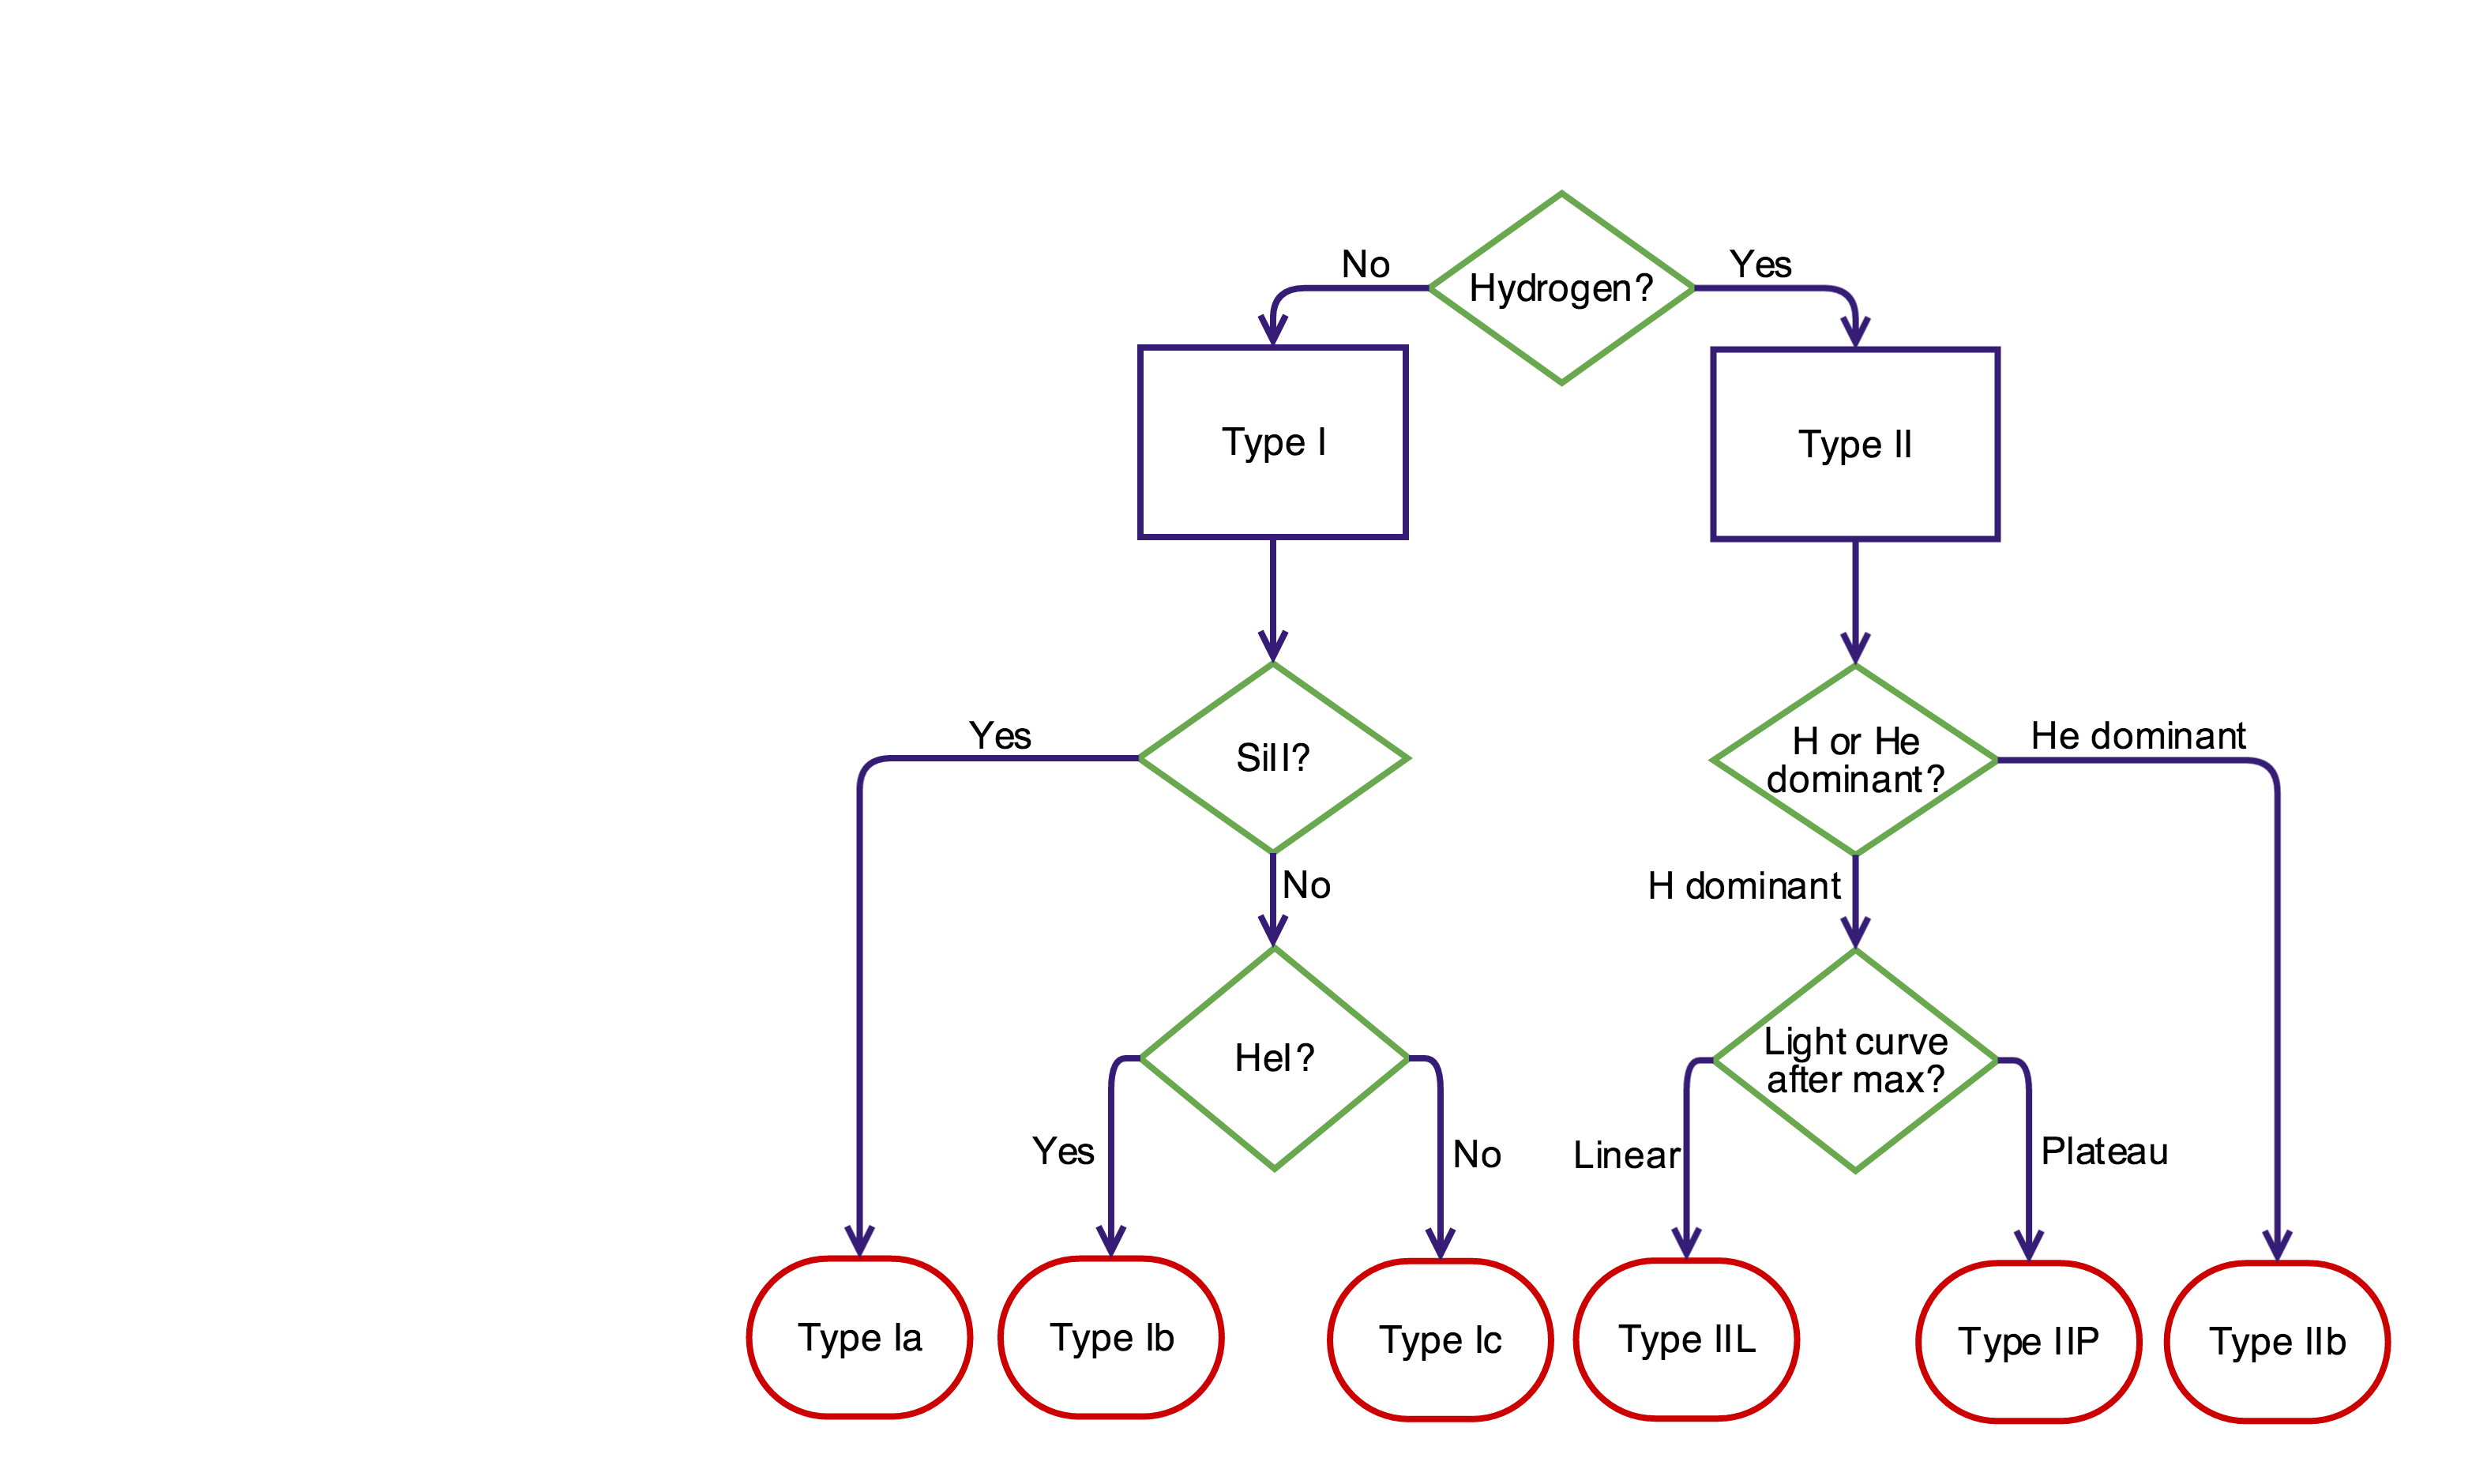
\includegraphics[clip=true, scale = 0.2, trim= 930 50 55 210]{chapters/chapter1/figs/sn_classification.png}
\caption{A flowchart summarising the supernova classification scheme}
\label{intro:fig:sn_class}
\end{figure}

If the initial classification is Type I then all further sub-classifications depend solely on the properties of the early spectra (a few days after explosion) as detailed in Figure \ref{intro:fig:sn_class}.  Type II supernovae are somewhat more complex in their categorisation.  After classification as a Type II, further subdivisions depend on the dominance of hydrogen or helium in \textit{later} spectra.  Helium dominant supernovae are classified as Type IIb and hydrogen dominant supernovae are classified as either Type IIL (those which have a linearly decaying light curve after maximum light) or Type IIP (those that exhibit a plateauing light curve after maximum light).  Type IIn supernovae are omitted from the summary presented in Figure \ref{intro:fig:sn_class} as they cannot be classified straightforwardly via a bifurcating process.  Type IIn supernovae will generally have strong emission lines, particularly hydrogen lines, often with complex profiles.  Crucially, the spectra of Type IIn supernovae do not exhibit the broad absorption features frequently seen in other types and instead contain narrow lines (hence Type IIn).  

\subsection{From Massive Stars to Remnants}

It is generally accepted that the progenitors of Type Ia supernovae are white dwarfs that exist in a binary system with another star.  The accretion of material from one star to another results in a thermonuclear explosion, a mechanism that is unique to Type Ia supernovae.  There have not been any observations suggestive of dust forming in the aftermath of a Type Ia supernova and I therefore do not consider these objects any further, focusing my attention solely on supernovae that explode via the core-collapse mechanism.  

Broadly, this process is initiated when a massive star ($\ge 8$\msun) starts to fuse heavier elements. The fusion of ever heavier elements generates increasingly less energy whilst also causing the mass of the core to increase.  Eventually, radiation pressure drops sufficiently that the core can no longer support itself against its own self-gravity and begins to collapse rapidly. Within milliseconds, the core reaches extremely high densities and, when it can no longer condense further, ``bounces" off itself causing  an immense shockwave to propagate outwards and a vast quantity of energy to be released via the expulsion of neutrinos.  Much of this complex process is still poorly understood and interesting models are currently being produced recreating these very early stages using a numerical approach.  Though the explosion mechanisms of CCSNe are largely beyond the scope of my work, some attention will be paid to these models later in this thesis since instabilities that arise in these early stages can influence the structure of the ejecta at later stages of its evolution.

For several hundred years after the explosion, the supernova (now a remnant) is in the free-expansion phase. During this phase, the mass and velocity of the expanding supernova massively exceed those of the surrounding medium, fortuitously allowing the behaviour of the remnant to be analysed as if it were expanding into a vacuum.  The shock radius during this phase may therefore be calculated simply as $R_s = v_s t$.  As the shockwave propagates through the ISM, interstellar material that has been compressed by the forward shock begins to accumulate.  At the same time a reverse shock wave begins to propagate back through the ejecta.  It is during this phase, which arises very soon after the initial explosion and lasts for a few hundred years, that the physical conditions in the ejecta are thought to be optimal for dust formation.  The phase ends when the mass of material ahead of the forward shock is of a similar magnitude to that behind and the mathematical treatment of its behaviour must be altered.


\subsection{Dust Formation in CCSNe}

Superficially, the formation of dust grains requires densities high enough for interaction between particles to take place, but temperatures that are cool enough to allow the grains to survive.  The theory that the ejecta of a CCSN in its free-expansion phase could provide these conditions  was first hypothesised by \citeauthor{Cernuschi1967} in 1967 and they have now long been thought to be potential dust factories \citep{Hoyle1970, Kozasa1991, Todini2001}.  

The formation of dust was originally thought to result from the stochastic process of classical nucleation whereby particles coalesce to form the seeds of dust grains.  These seeds become the nucleation sites from which grains are ultimately born through the aggregation of further particles.  Various models of dust formation in the ejecta of CCSNe have used this approach \citep{Kozasa1989, Todini2001,Nozawa2003, Schneider2004}.  

More recently, several models of dust formation in CCSNe that consider the effects of chemistry on the growth of dust grains have been published.   These models consider the chemical composition of the gas and include chemical reaction rates thereby considering the manner in which molecular evolution influences dust grain formation and growth rates \citep{Cherchneff2009, Cherchneff2010, Sarangi2013, Sarangi2015}.

Models using both methods have predicted dust masses of the order of 0.1-1\msun of dust forming within the ejecta of CCSNe of progenitor masses between 12-40\msun within the first few years after the initial explosion.

\subsection{The Three Signatures of Dust}
\label{three_sigs}
The presence of dust in the ejecta of CCSNe can be indicated by three main signatures: 

\subsubsection{A decrease in the light curve} 
As the dust begins to form in the ejecta, UV and optical light is absorbed by the dust causing a decrease in the light curve at these wavelengths.

\subsubsection{Excess IR emission}
An increase in emission in the IR occurs contemporaneously with the decrease in the UV-optical light curve.  A thermal MIR excess is caused by warm dust and an excess in the far-IR and sub-mm is the result of cold dust.  The increase in emission in these wavelength can be caused by newly-formed dust condensing in the ejecta but can also be a result of the illumination of pre-existing dust

\subsubsection{Blue-shifted line profiles}
Finally, the onset of the formation of dust can cause an asymmetry in line profiles in the optical and IR.  The absorption and scattering of optical or near-IR radiation by newly-formed dust within the ejecta can result in an asymmetry between the red and blue shifted components, with redwards 
emission from the far side of the ejecta undergoing greater absorption and resulting an overall shift of the profile to the blue.
\\

\noindent All three of these signatures have been discussed in detail over the timeline of this subject but the focus has been on using the excess IR emission seen in the SED of CCSNe to determine quantitatively dust masses in these objects.  This approach has resulted in a lively debate regarding the quantities of dust that CCSNe are capable of producing.
 
\subsection{The Dust Mass Debate}

%%MAYBE MORE DETAIL HERE %%%%
Over the past two decades, several high redshift galaxies  have been found to contain significant masses of dust \citep{Omont2001, Bertoldi2003, Watson2015}.  CCSNe are one of the few potential sources that could contribute large quantities of dust at early epochs. However, 
observations over the last decade at mid-infrared (MIR) wavelengths of 
warm dust emission from CCSNe has suggested that the quantities of ejecta-condensed dust 
produced during the first 1000 days were typically $\leq$ 10$^{-3}$~M$_\odot$  
\citep{Sugerman2006, Meikle2007, Kotak2009, Andrews2010, Fabbri2011}.  This is much less than the 0.1-1.0~M$_\odot$ of dust per CCSN  
estimated to be needed  in order to account for the masses observed \citep{Morgan2003, Dwek2007}.  These observations would indicate that other early-time sources of dust must be found.

 However, recent {\em Herschel} far-IR and sub-mm observations of  several young supernova remnants have revealed cold dust  masses as high as 
0.2-0.8$M_{\odot}$, resulting in a 
re-evaluation of the rate of dust production by CCSNe and a renewed focus on these objects as sources of dust \citep{Barlow2010, 
Matsuura2011, Gomez2012}.

\subsubsection{SN 1987A}


%more waffle on sn1987a

Critical to this field has been the study of SN 1987A.   This supernova is one of the most studied objects in the history of astronomy and has been observed almost continuously since it exploded 28 years ago.  The reason for this is its proximity.  At only ~50pc away, it has allowed for some exceptionally well-resolved spectral and photometric observations.  Neutrinos from its explosion were even detected at three different observatories .  As such, it has yielded results and insight that would not have been possible otherwise and is a key to understanding the formation and evolution of dust in CCSNe.

It is of no surprise therefore that this object has been central to the debate.  \citet{Lucy1989} was the first to suggest the presence of dust in SN~1987A {\em Herschel} observations of SN~1987A were the first to suggest the presence of cold dust in any supernova.



\subsection{Motivation}
%- call something else
It is seems increasingly likely that CCSNe do indeed produce significant quantities of dust.  However, there remain a large number of outstanding challenges to consider.  Firstly, there are still only a very small number of supernovae that have been observed to have sizeable masses of dust present in their ejecta.  If further CCSNe were also shown to have formed large quantities of dust then  the already shifting opinion might start to become consensus.  Other points to consider regarding dust formation and evolution in CCSNe include the nature of the dust (composition, grain size, grain shape etc.) which is still largely unclear, as is the extent to which it is destroyed or sputtered after its initial formation.  Related to this is the uncertainty of the dust formation rate in the ejecta and the issue of where this formation takes place.  These are all interesting questions that call out for answers.  

The {\em Hershel} dust mass estimates were based on fitting dust SEDs that peaked at far-IR wavelengths. Unfortunately, following the end of the {\em Herschel} mission in 2013, there is likely to be a long wait for far-IR facilities with comparable or better sensitivities than {\em Herschel} to become available.  Without data, this methodology is temporarily ineffectual.  This provided an incentive to make use of alternative methods to estimate the dust masses that form in supernova ejecta.

\section{Dust-Affected Line Profiles}

%%MORE HERE

 \citet{Lucy1989} identified a progressive blue-shifting of the [O~{\sc 
i}]~$\lambda$6300,6363~\AA\ doublet from SN~1987A between days 529 and 739 
after outburst, with the doublet in the later spectrum being blue-shifted 
by $\sim 600 $~km~s$^{-1}$. Since then, such red-blue asymmetries have 
been frequently observed in the late-time ($ > 400$ days) spectra of 
supernova ejecta and there is now a growing database of such observations (e.g.
\citet{Lucy1989,Fabbri2011,Mauerhan2012,Milisavljevic2012}).


The purpose of my work has been to develop a new approach to determining dust masses in supernovae, with the aim of providing an alternative to SED fitting for the future and of providing corroborating or contradicting evidence of past results.  I looked to exploit the third signature of dust formation in supernovae, namely the red-clue line asymmetry observed in optical and IR line profiles.  Though this feature has been discussed a length by numerous authors (REFERENCES) it has very rarely been quantitatively measured or modelled.

I have sought to construct a Monte Carlo based code that numerically models this feature in the spectra of SNe in order to quantitatively determine dust masses formed at a variety of epochs post-explosion, additionally seeking to place constraints of the composition and grain size distributions of the newly-formed dust.

\subsection{Observing}

Numerous telescopes have recorded spectra of CCSNe in the optical and IR, some with extremely high resolution.  The Anglo-Australian Telescope (AAT), the Cerro Tololo Inter-American Observatory (CTIO), the Hubble Space Telescope (HST) and the Very Large Telescope (VLT) have all observed several supernovae in the optical including SN 1987A.  Other telescopes such as  the two Gemini Multi-Object Spectrographs (GMOS) have also taken spectra of numerous CCSNe.

Advances in digital storage have allowed for spectral and photometric observations to be made easily available online.  Many observatories now publish their recent observations online in archives and are working to upload observations that pre-date file sharing services.  Much of the data used in this thesis was obtained from these archives. 

\subsection{Modelling}
Need to think about what i actually need to consider in this section.

- dust absorption, scattering and reemission in the IR
- raditaive transfer and independence of optical properties and temp meaning do not need to fully solve rad tran problem
- mie theory deets?  how is it solved and what is the theory?
- assumptions of isotropy?  scattering matrices?
\subsection{Mie Theory}
\label{scn:mie_theory}
In order to truly understand observations that are a product of dust, we must first understand those facets of a dusty medium that determine its interaction with incident radiation.  Dust grain radii are often of a similar order of magnitude to the wavelength of that incident radiation and so may be analysed from an optical perspective using Mie Theory.  Mie Theory is a mathematical solution to Maxwell's equation that describe how light is scattered off a small particle.  In combination with the optical properties of the medium, this allows for a precise determination of the extinction and scattering efficiencies of a given environment.  Conveniently, this allows for the straightforward modelling of a dusty medium and it is this calculation that I exploit in my models.  Mie Theory assumes particles to be spherical, an assumption which is a potential issue since grains may be crystalline, fluffy or extremely amorphous.  This issue is addressed later in this thesis.



\section{Content Of This Thesis}
And relate to your current work - give an overview of the work and what you did as well as the structure of the thesis - see Jo's for example.

\clearthesisemptydoublepage
  \chapter{A Description of DAMOCLES}\label{chp:chp2}

%\begin{flushright}
%  {\em QUOTE GOES HERE }\\
%
%\ \
%
%\normalsize
%{AUTHOR}  
%\end{flushright}


\section{Monte Carlo Methods}

\noindent{The name ``Monte Carlo" describes a class of modelling techniques that employ a stochastic approach to simulating mathematical and physical situations that are otherwise difficult or impossible to solve.  By repeatedly sampling random numbers from a probability distribution, numerical results to non-analytic problems may be obtained.  The approach was first used by researchers at Los Alamos in the late 1940s who adopted the method to model the transport of neutrons \citep{Metropolis1949}.  It is from the code name for this project, ``Monte Carlo", that the methods derive their name.}

As the available computing power increased over the following decades, Monte Carlo methods became more and more useful as a means of solving complex problems and are now used widely across numerous fields including mathematics, statistics, engineering, finance, the physical sciences and many others.  The nature of the approach means that they are particularly well-suited to problems with multiple degrees of freedom, and especially when any of these degrees are coupled.  By using random numbers to represent quantities that parametrise a physical problem, a solution to the problem may be sought using a pseudo-random number generator.   It must be the case that the quantities that characterise the problem may be represented by a continuous distribution in the range [0,1] in order that the randomly generated numbers may be translated into physical properties \citep{Shreider1966}.  

Having thus obtained a random set of physical parameters, a model is constructed and an output - a ``possible outcome" - is obtained.  By repeatedly iterating this process with new randomly-generated inputs each time, many possible outcomes are produced and a probability distribution is built up.  The interpretation of the outputted probability distribution is dependent on the manner of utilisation of the Monte Carlo method.  For example, the procedure may be used to find the mean-free paths of millions of energy packets where the resulting probability distribution of the final frequencies of the packets is equivalent to an energy distribution.  This is the process that I make use of and I will discuss it in more detail throughout this chapter.

More recently Monte Carlo methods have been applied to Bayesian statistical analyses that seek to uncover a complete multidimensional probability distribution describing the parameter space of a particular model.  The intention is to derive not just a well-fitting model but to understand how variations in a given parameter affect the likelihood that the model is representative of the data.  These investigations of parameter space generally adopt a Markov Chain Monte Carlo (MCMC) approach.  Where a Monte Carlo method generates a sample from a required distribution, a MCMC technique draws samples according to a predefined set of rules that result in a sequence of samples called a Markov Chain.  These methods allow for a more intelligent and efficient sampling of parameter space \citep{Metropolis1953, Hastings1970, Gilks1996}.  

Clearly, Monte Carlo simulations are limited by their finite nature and will never produce a perfect solution.  However, this does not mean that Monte Carlo simulations are lacking in rigour.  It may be shown that the error in a Monte Carlo model is approximately $\sim \frac{1}{\sqrt{n}}$ for large $n$, where $n$ is the number of quanta used in the simulation \citep{Press2007}.  The error may therefore be made as small as required by increasing the number of quanta used in the simulation subject to the restrictions of computing time and expense.

In the next section, I discuss the use of Monte Carlo methods as applied to radiative transfer problems and specifically to DAMOCLES.  I discuss the computational aspects of my work and the architecture of the code in section \ref{damocles_struct} before finally discussing the limitations of the code and its potential for future developments in section \ref{limitations}.

\section{Radiative Transfer and the Monte Carlo Method}
\label{rt}

The application of Monte Carlo codes to radiative transfer problems in astrophysics has a strong history.  Numerous codes that utilise this stochastic methodology have been written in the past few decades in order to model the transport of energy packets through various media, for example Cloudy \citep{Ferland2013}, Hyperion \citep{Robitaille2011}, LIME \citep{Brinch2010}, Mocassin \citep{Ercolano2003, Ercolano2005}, RATRAN \citep{Hogerheijde2000}, SKIRT \citep{Baes2003}, TORUS \citep{Harries2000} and many others.  The energy to be transported throughout the region of interest is discretised into packets and the path of each packet is calculated according to the properties of the environments that it passes through during its lifetime.  Collating the escaped packets at the end of the simulation produces an energy distribution that may be compared to observed photometric or spectral data. 

In addition to numerous codes that treat the continuous emission and absorption of energy in dusty environments in order to produce and fit spectral energy distributions (SEDs), there also exist several Monte Carlo radiative transfer codes that model the transfer and interaction of line emission through a 3D nebula in order to produce a synthetic spectrum (e.g. Brute \citep{Thomas2003} and ARTIS \citep{Kromer2009}).  These  models frequently employ an approximation known as the Sobolev approximation \citep{Sobolev1957} to treat the absorption and scattering of photons.  This method allows spectral lines in media moving with high velocity gradients to be treated more simply by solving the radiative transfer equation locally under the assumption that the macroscopic velocity gradient is more important than the thermal line width.  Models of supernovae have been produced using both approaches and well-fitting spectra and SEDs have been generated but never, according to the best of my knowledge, has the Monte Carlo methodology been employed to produce sophisticated models of individual line profiles in expanding dusty regions.  In this new code, DAMOCLES, we seek to apply the technique to an expanding dusty medium in order to consider the effects of dust on a single emitted line profile.  

Previous work by Leon Lucy has considered the problem of computing the spectra of supernovae using Monte Carlo techniques \citep{Lucy1987,Lucy1999,Lucy2002,Lucy2003,Lucy2005c,Lucy2005b}.  In particular Lucy and colleagues consider dust-induced asymmetric line profiles in the ejecta of CCSNe and they have published results derived both analytically and using simple Monte Carlo simulations \citep{Lucy1989,Lucy1991}.  These simulations appear to be the only published instances of a numerical approach to studying this type of spectral feature.  The DAMOCLES code adopts the same technique as the original modelling by Lucy et al. but allows for a considerably more complex treatment of the composition, geometry and motion of the dusty medium.

Radiative transfer methods as applied to supernovae generally treat a wide wavelength range and seek to conserve the total energy.  In the case of SED modelling, this is often achieved by dividing the total energy into packets of equal weight and energy, and iteratively determining the temperature and ionisation structure.  In this work, the approach we adopt is somewhat simpler as only a very narrow wavelength range need be considered.  Rather than seeking to conserve the total energy, we assume that any packet absorbed by dust would be re-emitted outside the wavelength range of interest and thus no longer contributes to the resulting line profile.  Any absorbed packet is therefore removed.  In addition to this, the absorption and scattering of radiation by dust is assumed to be independent of temperature and there is therefore no need to calculate grain temperatures throughout the nebula.  Similarly, the use of the Sobolev approximation (described above) is unnecessary here as the lines treated are assumed to be optically thin. 

The subtleties of the problem we consider here lie in the treatment of an atmosphere expanding as fast as 10\% of the speed of light, and in the complexities of the dusty medium itself.  Lorentz transforms must be carefully applied in order that packets experience the appropriate degree of frequency shifting on their original  emission and at each subsequent scattering event.  In this respect, the code is analogous to Monte Carlo radiative transfer models of electron scattering published by \citet{Auer1972} and \citet{Hillier1991}.  Indeed, similar features are observed in the outputs of both.

Throughout this section, I will describe the principles, assumptions and techniques adopted in the production of DAMOCLES (see Figure \ref{fig:flowchart}) before I move on to address the mechanics and architecture of the code itself.  DAMOCLES stands for \textbf{D}ust-\textbf{A}ffected \textbf{M}odels \textbf{O}f \textbf{C}haracteristic \textbf{L}ine \textbf{E}mission in \textbf{S}upernovae.


\begin{figure}
\centering
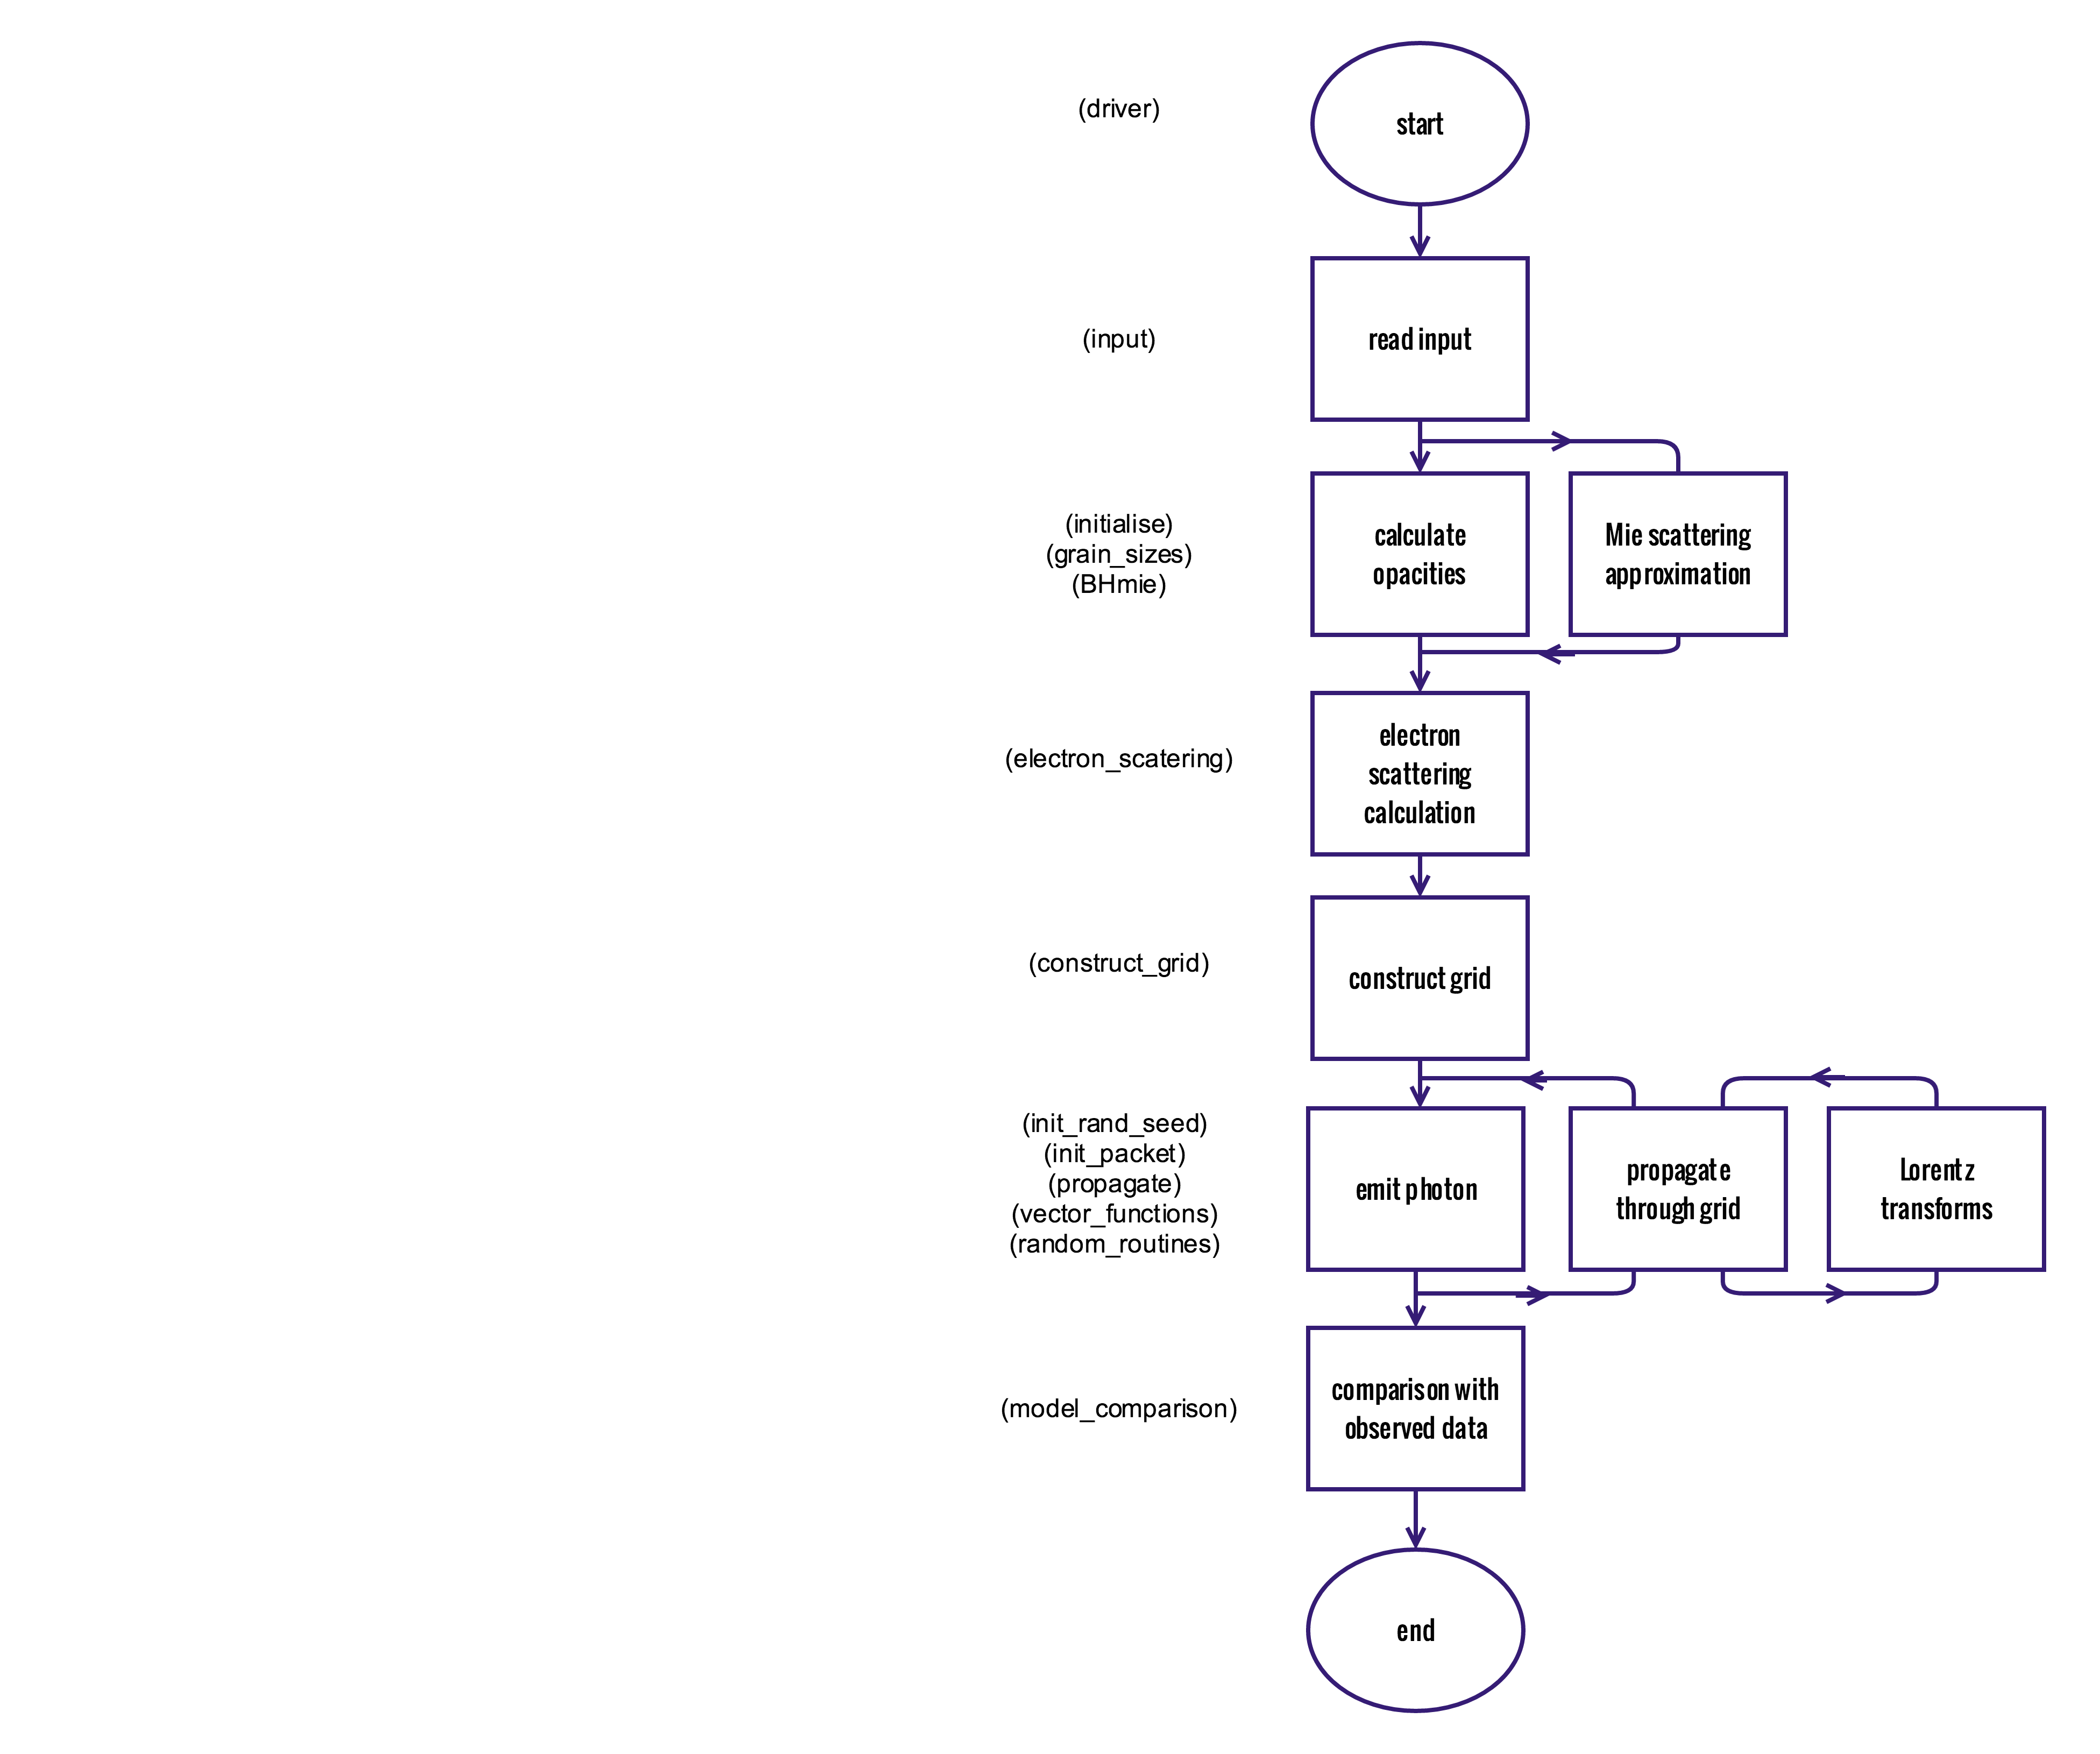
\includegraphics[scale=0.185, trim=650mm 25mm 8mm 25mm]{chapters/chapter2/code_flow.png}
\caption{A flowchart representing the sequence of processes that take place in the DAMOCLES code.  The modules involved at each stage are given in parentheses.}
\label{fig:flowchart}
\end{figure}



\subsection{Energy Packets}

The fundamental principle underlying the Monte Carlo approach to the transport of radiation throughout a dusty nebula is that the radiation is discretised into packets.  Each of these packets is then propagated throughout the nebula and ultimately contributes a fraction of the final energy distribution.  At the start of the simulation, each packet is assumed to consist of $n$ photons of frequency $\nu_0$, the rest frequency of the monochromatic emission line to be modelled.  All packets therefore begin life with initial energy
\begin{equation}
E_0=nh\nu_0
\end{equation}

where $h$ is Planck's constant.  As the packets move through the ejecta, they are scattered off high-velocity dust grains and after each scattering event the frequency of the packet is altered.  In Monte Carlo simulations that model non-moving atmospheres, packets are usually taken to be of constant energy.  When the frequency of a packet is altered after an event, the energy of that packet is kept constant and the number of real photons contained within it assumed to change.  However, in the case of dust scattering, the number of real photons is conserved and thus the energy of the packet is altered.  This is most easily achieved by weighting each packet over all scattering events as 
\begin{equation}
w_p=\prod_{scat} \frac{\nu'}{\nu}
\end{equation}

\noindent where $w_p$ is the weight of the packet and $\nu$ and $\nu'$ are 
the frequencies of the packet before and after the scattering event 
respectively.  The final energy of each packet is then $E =w E_0$, where $E_0$ is the initial energy of the packet.  The final dust-affected line profile is compiled by adding the total energy of all packets in a specific frequency bin in order to produce a histogram.

In these models, unlike fully self-consistent SED radiative transfer models, there is no requirement that the total energy be conserved.  We drop this traditional requirement since radiation that is absorbed by dust is re-emitted outside of the wavelength range of interest and thus no longer contributes any flux to the resulting line profile.  Packets that are absorbed may be safely removed from the simulation.

\subsection{Initialisation and the Grid}

The supernova ejecta is approximated by a three-dimensional cartesian grid, each cell of which is assumed to have uniform density and composition.  By default, the ejecta occupies a shell between inner radius $R_{in}$ and outer radius $R_{out}$. The grid extends from $-R_{out}$ to $+R_{out}$ in each of the three axes.  Each side is split into the same number of divisions and thus each cell is a cube of volume $R_{out}^3/n_{div}^3$ where $n_{div}$ is the number of divisions along each axis and is specified by the user.  For the remainder of this thesis, a spherically symmetric situation is assumed and in all modelling and testing the grid is constructed in this manner.  However, there are no assumptions of symmetry in the code and a cartesian grid was adopted in order to allow for arbitrary geometries to be modelled in the future e.g. ellipsoidal or toroidal ejecta distributions.

\subsubsection{Smooth power-law density distributions}

Both gas and dust are by default assumed to have a power-law distribution declared as  $\rho(r) \propto r^{-\beta}$ between $R_{in}$ and $R_{out}$.  The distribution of gas determines the emissivity distribution and thus the starting positions of the packets in the simulation (see section \ref{sctn:em_prop}).  However, after the initial emission of energy packets, the gas plays no further role in the simulation as only interactions with dust grains are of interest here.  By default, the dust is coupled to the gas and thus follows the same smooth power-law distribution previously described with exponent $-\beta$.  The dust density in each cell is therefore calculated as
\begin{equation}
\rho (r)= \frac{(3-\beta)M_{tot}}{4\pi (R_{out}^{3-\beta}-R_{in}^{3-\beta})} r^{-\beta}
\end{equation}


\noindent if $\beta \neq 3$, where $r$ is the radial distance from the centre of the cell to the origin and $M_{tot}$ is the total desired dust mass to model.  For the standard model with $\beta=2$ this becomes
\begin{equation}
\rho (r)= \frac{M_{tot}}{4\pi (R_{out}-R_{in})r^2}
\end{equation}

\noindent If $\beta = 3$ then the dust density in each cell is alternatively calculated as 
\begin{equation}
\rho (r)= \frac{M_{tot}}{4\pi \log (R_{out}-R_{in})r^{3}} 
\end{equation}

Any cell whose centre falls outside of the bounds of the supernova ejecta has dust density set to zero.  If the dust and gas are decoupled then the user must specify distinct profiles for the gas and the dust; that is, separate power laws must be declared and independent inner and outer radii specified.  The same process is followed but with separate power-laws for each component.  Including the capacity to specify the gas and dust distributions separately allows for more sophisticated modelling of, for example, circumstellar shells or dense cores of dust formation surrounded by more diffuse gas.

\subsubsection{Clumped geometries}

It is known from SED modelling that models of clumped environments produce very different results to environments assumed to have a smooth distribution of dust and gas (e.g. \citet{Bianchi2000,Ercolano2007,Owen2015}).  %Generally, in comparison to smooth models, clumped models tend to require more dust in order to reproduce a similar level of emission or absorption.  
The capacity for modelling a clumped dusty medium is therefore included in the code.  The fraction of the dust mass that is in clumps is declared ($m_{frac}$) and the total volume filling factor of the clumps ($f$) is also specified.  Dust that is not located in clumps is distributed according to a smooth radial power-law.  The clumps occupy  a single grid cell and their size can therefore be varied by altering the number of divisions in the grid.  They are distributed stochastically with probability of a given cell being a clump proportional to the smooth density profile (i.e. $p(r) \propto r^{-\beta}$).  The density of all clumps is constant and is calculated as 
\begin{equation}
\rho_{clump}=\frac{M_{clumps}}{V_{clumps}}=\frac{m_{frac}M_{tot}}{\frac{4}{3} f\pi (R_{out}^{3}-R_{in}^{3} )}
\end{equation}

\noindent where $M_{tot}$ is the total dust mass, $M_{clumps}$ is the total dust mass in clumps and $V_{clumps}$ is the total volume occupied by clumps.  $m_{frac}$ and $f$ are defined as above.

A grid of cubic cells of varying dust and gas densities is thus produced in readiness for packets to be transported through it.  Examples of smooth and clumped distributions of dust generated by DAMOCLES are presented in Figure \ref{fig:grid}.  A frequency grid is also established centred on the rest-frame frequency of the line to be modelled.



%\begin{figure}
%%		\centering
%\begin{subfigure}{0.4\textwidth}
%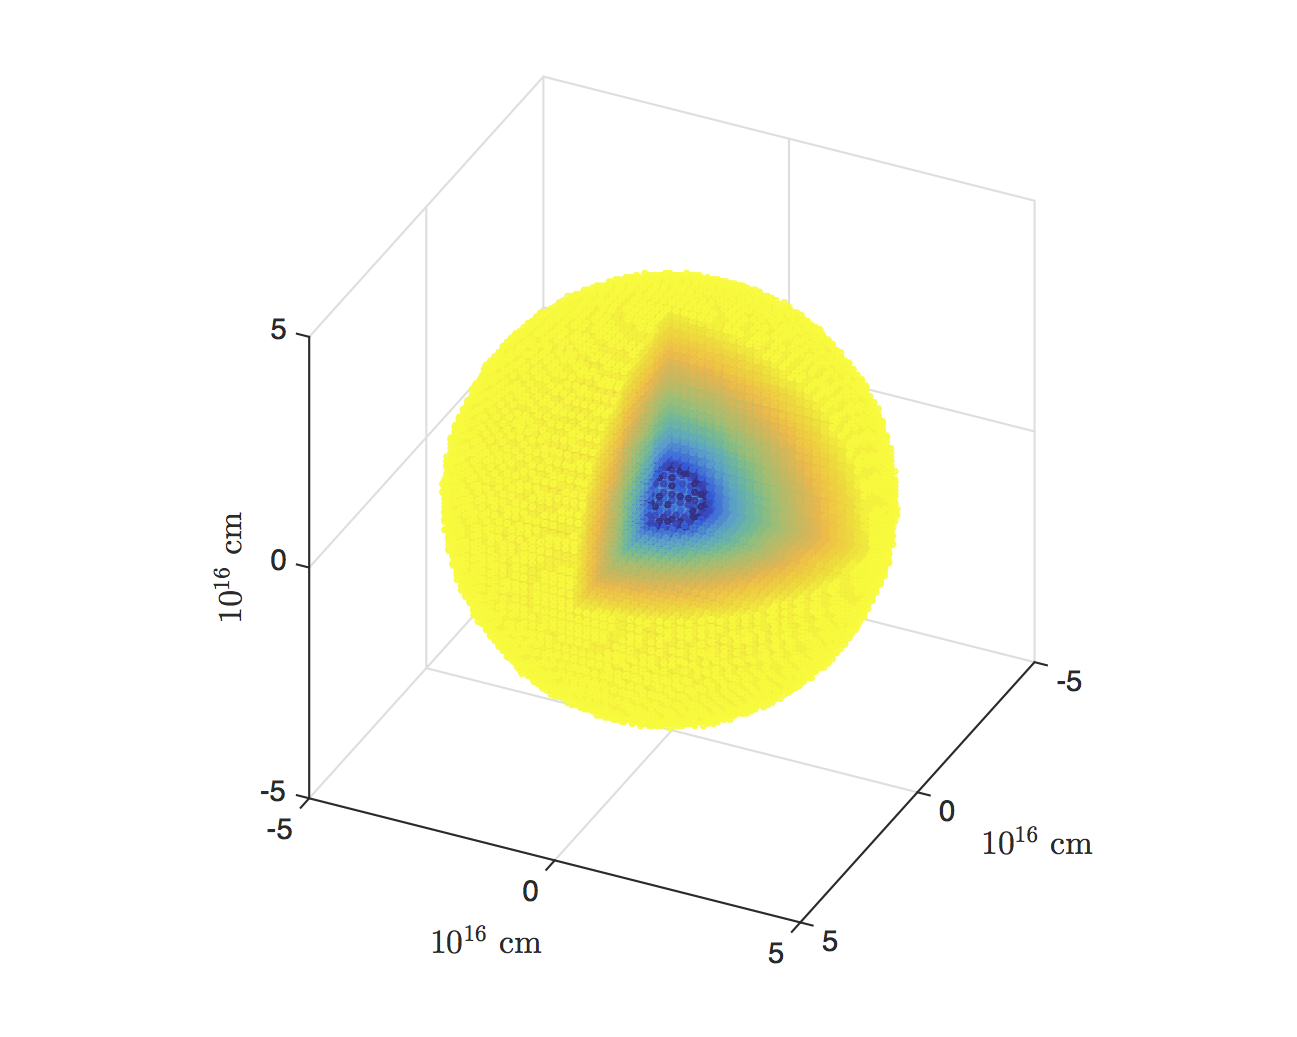
\includegraphics[scale=0.5, trim=35mm 5mm 34mm 5mm,clip=true]{chapters/chapter2/smooth_grid}
%\end{subfigure}
%\hspace{18mm}
%\begin{subfigure}{0.4\textwidth}
%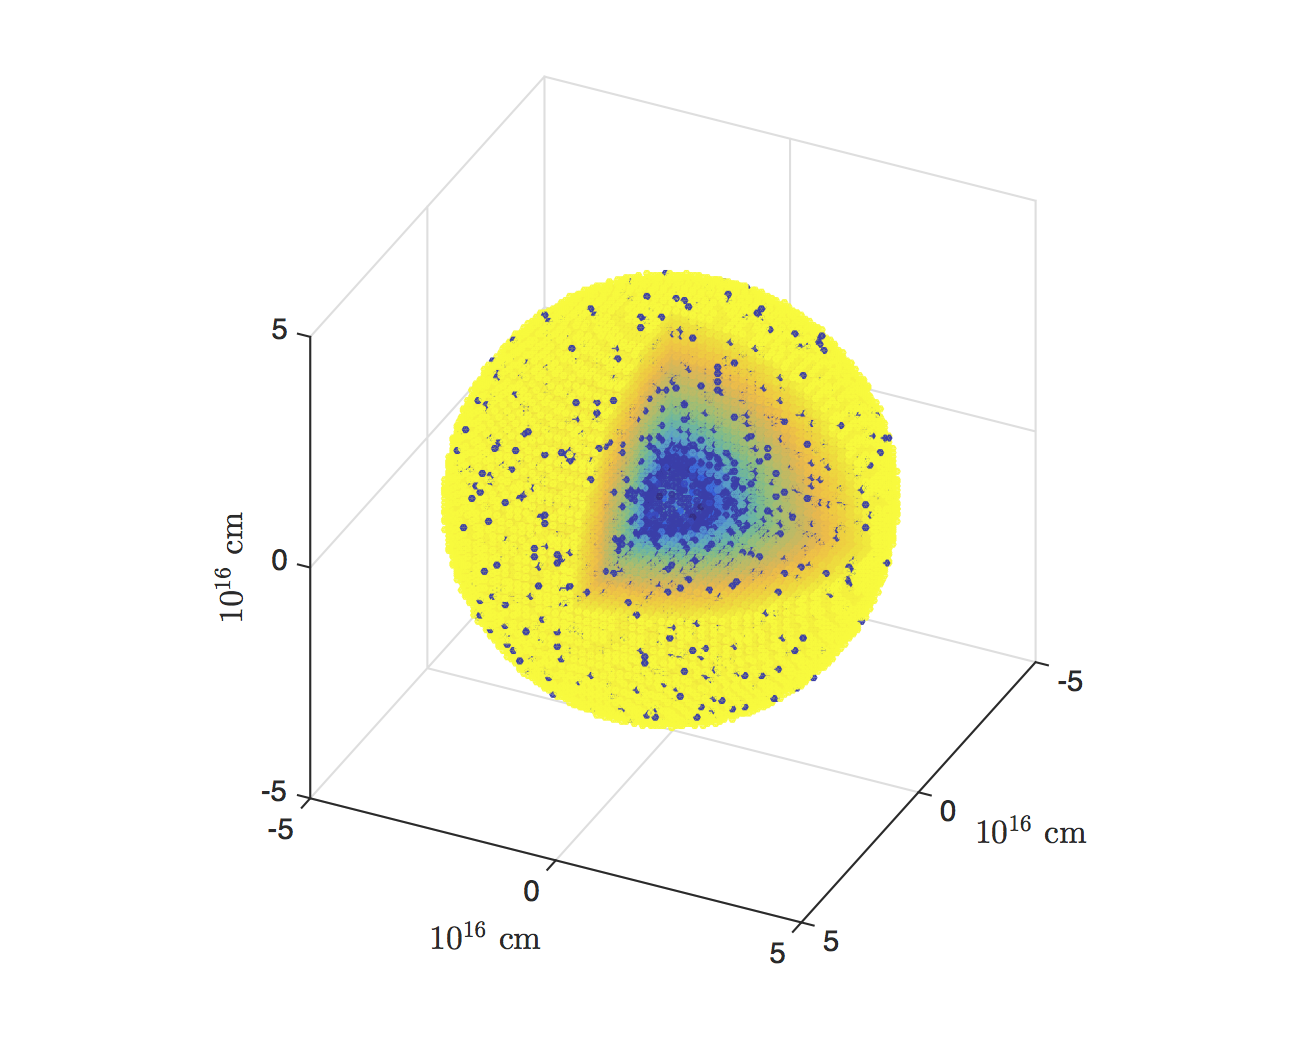
\includegraphics[scale=0.5, trim=35mm 5mm 34mm 5mm,clip=true]{chapters/chapter2/clumped_grid}
%\end{subfigure}
%\caption{3D representations of the grid generated by DAMOCLES.  A smooth distribution is shown on the left and a clumped distribution on the right.}
%\label{fig:grid}
%\end{figure}

%%%%LOW RES VERSION%%%%%%%%
\begin{figure}
%		\centering
\begin{subfigure}{0.4\textwidth}
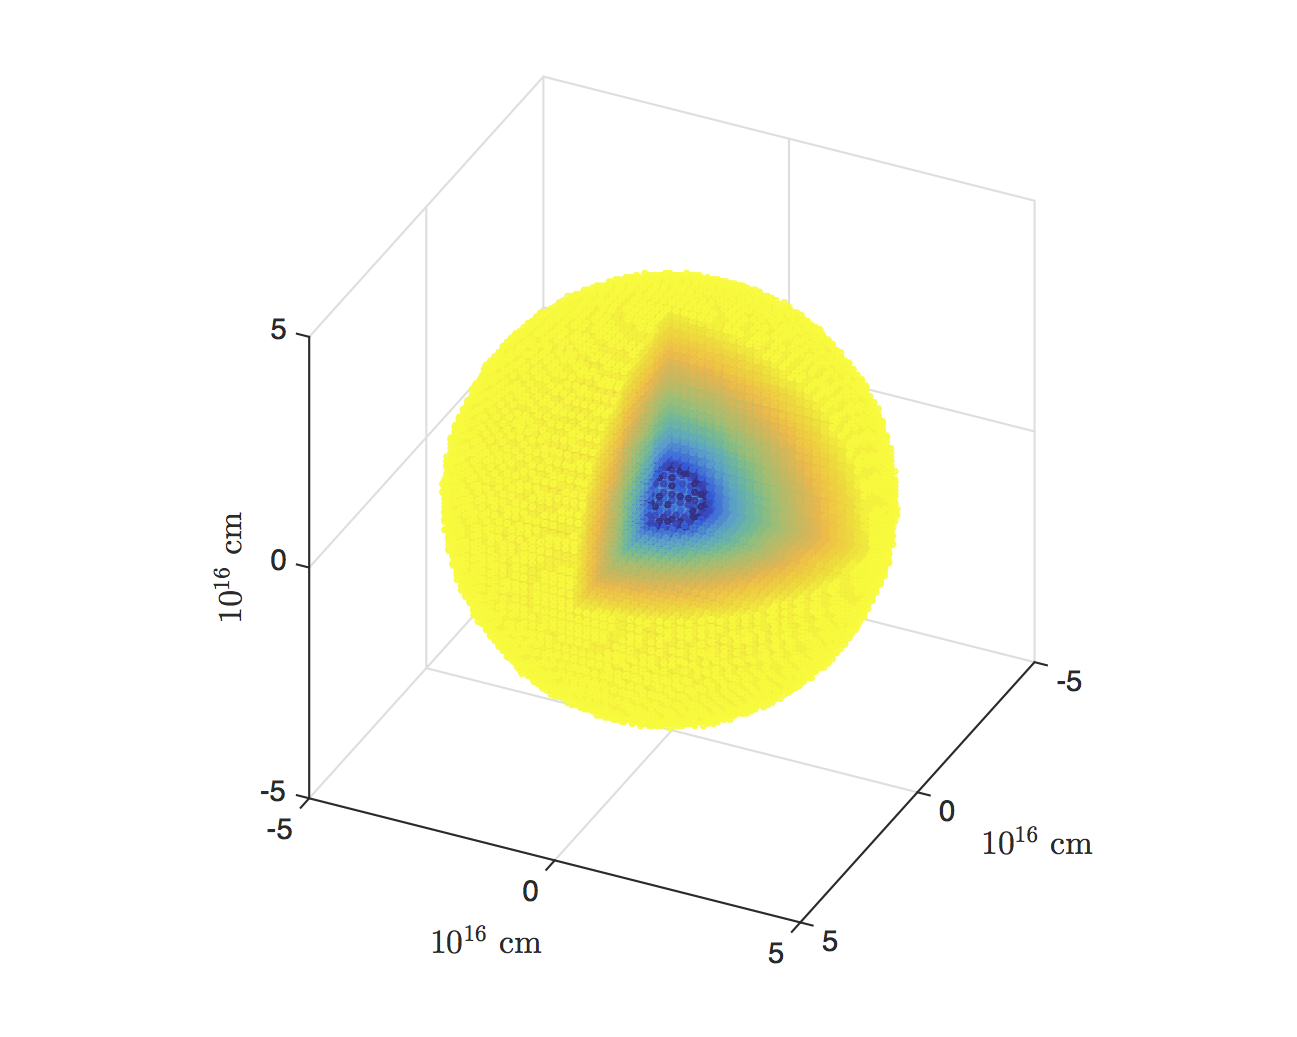
\includegraphics[scale=0.5, trim=35mm 5mm 34mm 5mm,clip=true]{chapters/chapter2/smooth_grid.png}
\end{subfigure}
\hspace{18mm}
\begin{subfigure}{0.4\textwidth}
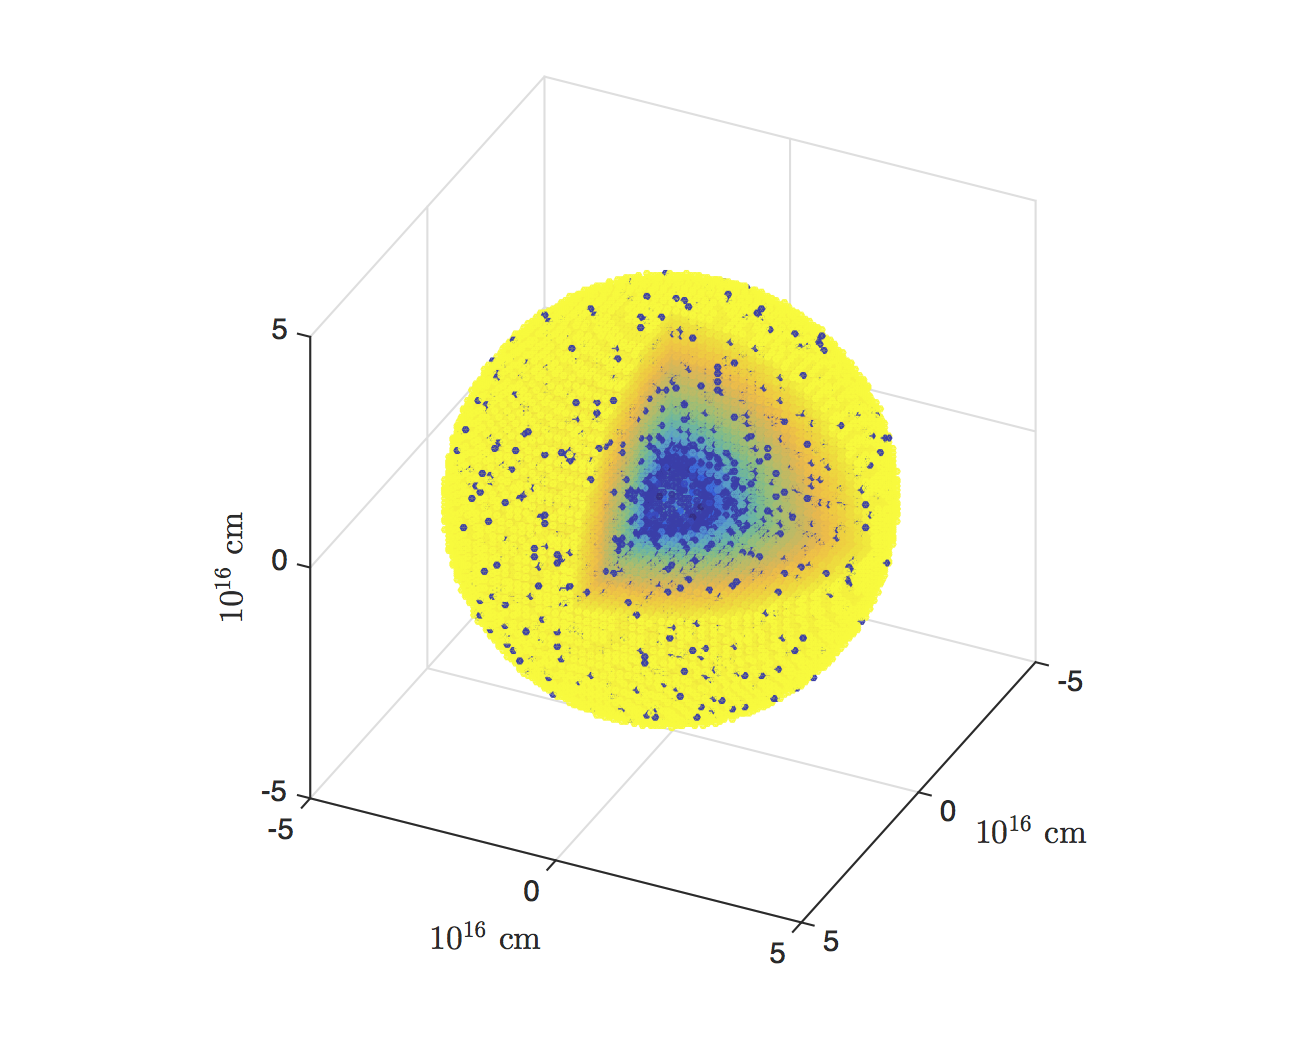
\includegraphics[scale=0.5, trim=35mm 5mm 34mm 5mm,clip=true]{chapters/chapter2/clumped_grid.png}
\end{subfigure}
\caption{3D representations of the grid generated by DAMOCLES.  A smooth distribution is shown on the left and a clumped distribution on the right.}
\label{fig:grid}
\end{figure}


\subsection{Properties of the Dusty Medium}
\label{scn:grainsize}
Dust of any composition may be used for which optical data are available.  The relative abundances of the species must be declared in an input file accompanied by a grain radius distribution (specified as a grain radius range and power-law) for each species.  Files detailing the optical data ($n$ and $k$ values) for the chosen dust species are also declared at the start of the code.  For each pairing of wavelength $\lambda$ and grain radius $a$, a Mie scattering routine is employed to calculate $Q_{abs}(\lambda,a)$ and $Q_{sca}(\lambda,a)$ from the refractive index $n+ik$.  These values are calculated for every species across the wavelength and grain radius ranges of interest.  I have described the mathematics of converting the refractive index into scattering and absorption efficiencies using Mie theory in detail in the introduction to this thesis (see Section \ref{scn:mie_theory}).


Ultimately, the overall scattering and absorption opacities in each grid cell must be known and so a weighted summation over $Q_{abs}(\lambda,a)$ and $Q_{sca}(\lambda,a)$ is performed.  The number density in each cell must first be calculated as 
\begin{equation}
\label{eqn:density}
n_d = \rho/m_{av}
\end{equation}

\noindent where $m_{av}$ is the average mass of a grain: 
\begin{equation}
\label{eqn:Mav}
m_{av}=\sum_i \sum_a \frac{4}{3} \pi a_i^3 \rho_{g,i} w_i(a) x_{M,i}
\end{equation}

\noindent $\rho_{g,i}$ is the density of the grain for species $i$ (specified with the optical data), $x_{M,i}$ is the relative abundance of species $i$ by mass and $w_i(a)$ represents the normalised weight of particles with grain radius $a$.  For a given power-law distribution of grain radii $n(a) \propto a^{-\alpha}$,   $w_i(a)$ is given by
\begin{equation}
w_i(a)=\frac{a^{-\alpha}}{\int_{a_{min}}^{a_{max}} a^{-\alpha} \, da}
\end{equation}

The relative abundances of the different species are declared by the user in terms of cross-sectional area ($x_{A,i}$).  From this, the relative abundances by volume ($x_{V,i}$) may be calculated as
\begin{equation}
x_{V,i}=(1+(x_{A,i}-1)^{\frac{3}{2}})^{-1}
\end{equation} 

\noindent giving the relative abundance by mass $x_{M,i}$ (used in Equation \ref{eqn:Mav})  
\begin{equation}
x_{M,i}=\frac{x_{V,i}\rho_{g,i}}{\sum x_{V,i}\rho_{g,i}}
\end{equation} 


\noindent For extinction, the total cross-section of interaction for extinction is then calculated as
\begin{equation}
\label{eqn:Cext}
C_{ext}(\lambda) = \sum_{i} \sum_a Q_{ext,i}(a,\lambda) w_i(a) \pi a_i^2 x_{A,i}  
\end{equation}

\noindent where the subscript $i$ denotes species $i$, $x_{A,i}$ represents the relative abundance of species $i$ by cross-sectional area and the summations are over species and grain radius.  The calculation of the cross-section of interaction for scattering $C_{sca}(\lambda)$ is performed in the same manner.  




Using equations \ref{eqn:density}, \ref{eqn:Mav} and \ref{eqn:Cext}, the dust opacity $\kappa_{ext}$ can then be calculated using the relationship
\begin{equation}
n_dC_{ext}=\rho \kappa_{ext}
\end{equation} 

The values of $C_{ext}(\lambda)$ and $C_{sca}(\lambda)$ are calculated for the full wavelength range at the start of the simulation as are the number densities in each grid cell.  As a packet passes through a grid cell, the optical depth $\tau$ is determined from the above quantities according to the wavelength of the current packet (see Section \ref{sctn:em_prop} for further detail on this process).  The above equations are discretised versions of continuous integral equations given in \citet{hulst1957} and \citet{tielens2005}.

%The Mie solution to Maxwell's equations may be approximated under certain conditions to allow for a computationally simple calculation of extinction, scattering and absorption efficiencies.  In particular, this approximation is appropriate in the regime where the wavelength of the incident radiation is of a similar order of magnitude to the diameter of a spherical scatterer.  It is therefore a helpful and suitable approximation to employ in DAMOCLES where we assume dust grains to be approximately spherical and of the order of $\sim 0.1 \mu$m in radius.  Further understanding of the properties of newly-formed dust in the ejecta of supernovae might be obtained by considering alternative approximations for these calculations in future, for example by considering a continuous distribution of ellipsoids in preference to solely spherical grains.  


\subsection{Emission and Propagation}
\label{sctn:em_prop}
The initial radiation field is inherently tied to the distribution of gas throughout the supernova ejecta.  The relationship between the emissivity and the gas density may vary under different regimes and therefore the emissivity distribution is also specified as a power-law with $i(\rho) \propto \rho^{q}$.  In general, however, the emissivity distribution is assumed to be proportional to the square of the local gas density ($i(r) \propto r ^{-2\beta}$), i.e. proportional to the product of the recombining 
ion and electron densities in the case of a recombination line or to the product of the atom and electron densities in the case of collisionally excited line emission.

The supernova ejecta is divided into shells between $R_{in}$ and $R_{out}$ and the number of packets to be emitted in each shell calculated according to the specified power-law emissivity distribution $i(r) \propto r^{-q\beta }$.  For each packet a location within the appropriate shell must be determined and a propagation direction sampled.  The initial propagation direction is sampled from an isotropic distribution as detailed in numerous publications (e.g. \citet{Wood2004}). Three random numbers in the range $[0,1)$ are sampled and these are translated into spherical coordinates as 
%\begin{equation}
\begin{align}
\label{eqn:isotropic}
\phi&=2\pi\eta \\
\theta&=\arccos(2\xi -1) 
\end{align}
%\end{equation}

\noindent where $\eta$ and $\xi$  are random numbers in the range $[0,1)$, $\phi$ is the azimuthal angle and $\cos \theta$ is the radial direction cosine.  The initial packet trajectory in cartesian coordinates is then given by 
\begin{align}
n_x&=\sin\theta\cos\phi \\
n_y&=\sin\theta\sin\phi \\
n_z&=\cos\phi
\label{eqn:isotropic2}
\end{align}

The process for sampling an initial position within the shell follows the same sampling process as described above  but a radial position must be sampled in addition to the two angular coordinates.  For a random number $\zeta$, the radial position $r$ is calculated as
\begin{equation}
r=R_i+\zeta(R_{i+1}-R_i)
\label{eqn:isotropic3}
\end{equation}
\noindent where $R_i$ is the inner boundary of the $i$\textsuperscript{th} shell.

In total therefore five random numbers must be sampled in order to generate an initial position and trajectory for a packet. At every subsequent scattering event, the packet is propelled with a new direction vector which is sampled from an isotropic distribution in the rest-frame of the particle with two newly generated random numbers in the manner described above.  

%I do not include forward-scattering matrices in the code since the effects of forward scattering by dust are so small as to be negligible and it is simpler and more efficient simply to assume isotropic scattering.  

Once a packet has been emitted into the nebula, it must be propagated through the grid until it escapes the outer bound of the ejecta $R_{out}$ or is absorbed.  In each cell that a packet passes through, a test must be performed in order to determine whether the packet passes through that cell and into the next or whether it is scattered or absorbed by a dust grain (i.e. an ``event" occurs).  The probability that a packet travels a distance $l$ without interacting is 
\begin{equation}
p(l)=e^{-n_d \sigma_{\lambda} l}=e ^{-\tau_{\lambda}} 
\end{equation}

\noindent where $n_d$ is the dust number density in the grid cell, $\sigma_{\lambda}$ is the extinction cross-section of interaction at wavelength $\lambda$ and 
\begin{equation}
\tau_{\lambda} = n_d\sigma_{\lambda} l = \rho \kappa_{\lambda}  l
\end{equation}

\noindent for constant $n_d$ and $\sigma_{\lambda}$ (as in a grid cell).  Note that $\sigma_{\lambda}$ is used to denote the cross-section of interaction for a given grain radius.  Where a grain radius distribution is adopted or multiple species are employed, the formula becomes $\tau_{\lambda} = nC_{ext,\lambda}l$ as described in Section \ref{scn:grainsize}.  The probability that a packet \textit{does} interact within a distance $l$ is therefore $1-e^{-\tau_{\lambda}}$.  The position at which the packet will be absorbed or scattered is then determined by comparing a randomly generated number in the interval [0,1) with this value.  In practice however, it is easier to sample from the cumulative probability distribution and use the generated number to calculate an optical depth as 
\begin{equation}
\xi = 1 - e^{-\tau_{\lambda}}  \implies  \tau_{\lambda}=-\log (1-\xi) 
\end{equation}

\noindent where $\xi \in [0,1)$ is a sampled random number between $0$ and $1$.  The properties of the cell as determined in Section \ref{scn:grainsize} are then used to determine the distance that the packet travels:
\begin{equation}
l=\frac{\tau_\lambda}{n_dC_{ext,\lambda}}
\end{equation}

 If the distance to be travelled by the packet is greater than the distance from its position to the edge of the cell then the packet is moved along its current trajectory $(n_x,n_y,n_z)$ to the cell boundary and the process is repeated.  Alternatively, if the displacement is not sufficient for the packet to escape the cell then an event occurs.  The packet is either scattered or absorbed with probability of scattering equal to the albedo of the cell
\begin{equation}
\omega=\frac{\sigma_{sca}}{\sigma_{sca}+\sigma_{abs}}
\end{equation}

If the packet is absorbed (the case if a randomly generated number is greater than the albedo $\omega$) then it is simply removed from the simulation as previously discussed.  If this is not the case, then the packet is scattered and a new trajectory is sampled from an isotropic distribution in the comoving frame of the dust grain.  The frequency of the packet is recalculated using Lorentz transforms as described in the next section and the process is repeated until the packet has either escaped the outer boundary of the supernova ejecta or been absorbed.  If the packet does escape, its weighted energy is deposited in the appropriate frequency bin.  Once all packets have escaped, the array of frequencies and fluxes produces the desired line profile.

\subsection{The Velocity Field and Doppler shifting}

At emission and at each scattering event the frequency of the packet is recalculated according to a radial velocity field 
\begin{equation} 
v(r) = v_{max}\frac{r^{\alpha}}{R_{out}^{\alpha}}
\end{equation}

\noindent where the maximum velocity, $v_{max}$, at the outer edge of the ejecta and the exponent of the velocity profile, $\alpha$, are declared in the input file.	

It is worth noting that if a constant mass loss rate is required, the exponent of the velocity profile and the exponent of the density profile are not independent.  A constant mass loss rate implies that $4\pi \rho vR^2  \propto k$, where $k$ is a constant, and thus for $v \propto r^\alpha$ and $\rho\propto r^{-\beta}$, we require that $\beta-\alpha=2$.  However, it is possible that the supernova event may have induced a mass-flow rate that is not constant with radius and thus both exponents may be declared independently.  It is also worth noting that for supernovae in their free expansion phase, as the majority are by the time of the onset of dust formation, the ejecta are expanding with a $v \propto r$ Hubble law expansion.

The outflow velocities in supernovae can be extremely high, of the order of a few percent of the speed of light.  Escaping radiation is therefore subject to significant Doppler shifting. At emission and at each scattering event, the frequency of a packet must be recalculated according to the velocity of the scattering grain.  When the packet is initially scattered, it has a frequency and a trajectory in the rest frame of the emitter. Both of these must be transformed to the observer's frame in order for the packet to be propagated through the grid.  The new direction and frequency in the observer's frame may be simply found by transforming the momentum 4-vector $\boldsymbol{P}$ which is defined as
\begin{equation}
\boldsymbol{P}=
\begin{pmatrix}
E \\
p_x \\
p_y \\
p_z \\
\end{pmatrix} =
\begin{pmatrix}
h \nu \\
h \nu x \\
h \nu y \\
h \nu z \\
\end{pmatrix}
\end{equation}


\noindent We may then derive $\boldsymbol{P'}$, the momentum 4-vector in the observer's frame using the relation
\begin{equation}
\boldsymbol{P'}=\Lambda \boldsymbol{P}	
\end{equation}

\noindent where 
\begin{equation}
{\Lambda}=
\begin{pmatrix} 
\gamma & -\gamma \beta_x & -\gamma \beta_y & -\gamma \beta_z \\
-\gamma \beta_x & 1+(\gamma-1)\frac{\beta_x^2}{\beta^2} & 
(\gamma-1)\frac{\beta_x \beta_y}{\beta^2} & (\gamma-1)\frac{\beta_x \beta_z}{\beta^2} \\
-\gamma \beta_y  & (\gamma-1)\frac{\beta_y \beta_x}{\beta^2} & 1+(\gamma-1)\frac{\beta_y^2}{\beta^2} 
& (\gamma-1)\frac{\beta_y \beta_z}{\beta^2}\\
-\gamma \beta_z & (\gamma-1)\frac{\beta_z \beta_x}{\beta^2} & (\gamma-1)\frac{\beta_z \beta_y}{\beta^2} 
& 1+(\gamma-1)\frac{\beta_z^2}{\beta^2} \\
\end{pmatrix}
\\
\end{equation}
\\
\\
\noindent and $\boldsymbol{\beta}=\frac{{\bf{v}}}{c}=(\beta_x,\beta_y,\beta_z)$,   $\beta=\lvert \boldsymbol{\beta}\rvert$ and $\gamma = \frac{1}{\sqrt{1-\beta^2}}$.
\\

In practice, the velocities considered are low enough that it is unnecessary to consider terms of order $O(\frac{v^2}{c^2})$ and thus ${\Lambda}$ may be reduced to
\begin{equation}
{\Lambda}=
\begin{pmatrix} 
1 & - \beta_x & - \beta_y & - \beta_z \\
- \beta_x & 1 & 0 & 0 \\
- \beta_y  & 0 & 1 & 0\\
- \beta_z & 0 & 0 & 1 \\
\end{pmatrix}
\\
\end{equation}

\noindent The new direction of travel and frequency in the observer's frame are therefore given by  
\begin{equation}
\nu'=\nu(1-x\beta_x-y\beta_y-z\beta_z) \\
\end{equation}
\begin{equation*}
\begin{split}
x'=\frac{\nu}{\nu'}(x-\beta_x) \\
y'=\frac{\nu}{\nu'}(x-\beta_y) \\
z'=\frac{\nu}{\nu'}(x-\beta_z) \\
\end{split}
\end{equation*}

For each scattering event, the packet must be transformed both into and out of the comoving frame. The reverse transform is applied by using the inverse Lorentz matrix $\Lambda^{-1}$ which is obtained by reversing the sign of $\boldsymbol{v}$.  Positive $\boldsymbol{v}$ is defined for frames moving away from each other and thus $\boldsymbol{v}$ is defined to be negative in the direction of the observer.

\begin{table}[htdp]
\caption{Values of $q_{H\alpha}(T)$ at three different temperatures as used by DAMOCLES.}
\begin{center}
\def\arraystretch{1.5}
\begin{tabular}{ c c c c}
\toprule
&&Temperature (K) & \\
\cmidrule{2-4}
& 5,000 & 10,000 & 20,000  \\
\midrule
$q_{H\alpha}$ (erg cm$^3$ s$^{-1}$)  & $6.71\times 10^{-25}$	&$3.56\times 10^{-25}$	&$1.83\times 10^{-24}$  \\
\bottomrule
\end{tabular}
\end{center}
\label{tb:q}
        \end{table}%

        \subsection{Electron Scattering}
        \label{scn:ES}

        As will be discussed in detail in chapter three, the effects of scattering on the shapes of line profiles can be quite pronounced and it is therefore important to consider the potential effects of electron scattering as well as those of dust scattering.  A simple treatment of electron scattering calculates electron densities using an estimated average temperature of either 5,000K, 10,000K or 20,000K.  An observed luminosity of $H{\alpha}$ is then used to calculate the optical depth to electrons.  The overall optical depth within each cell is calculated as $\tau = \tau_{dust}+\tau_{e}$, with $\tau_{e}=0$ if electron scattering is not activated.  The electron scattering optical depth, $\tau_e$, in a given cell (with constant properties therein) is calculated as 
        \begin{equation}
        \tau_e =  n_e \sigma_t l
        \end{equation}
        
        \noindent where $n_e$ is the electron density in that cell,  $\sigma_t$ is the Thomson cross-section of interaction for an electron and $l$ is the distance travelled.	
        In order to calculate this value, the electron density in each cell must be known.  We assume that the electron density is the same as the ion density and that both are distributed according to the gas density distribution such that 
        \begin{equation}
        \label{eqn:es_distn}
        n_e(r) = Kr^{-\beta}
        \end{equation}

        \noindent  where $K$ is a constant.  The value of $K$ must be determined from the total H$\alpha$ luminosity.  We follow the formalism described by \citet{Osterbrock2006} in order to estimate the electron density from the total H$\alpha$ luminosity ($L_{H\alpha}$). $L_{H\alpha}$ is given by
        \begin{align}
        L_{H\alpha} =& \int _0 ^{\infty} n_p(r) n_e(r) E_{H\alpha} \alpha^{eff}_{H\alpha}(T) ~ \, 4 \pi r^2 \, dr  \\
        =& \int _{R_{in}} ^{R_{out}} n_p(r) n_e(r) q_{H\alpha}(T) ~ \, 4 \pi r^2 \, dr \label{eqn:es_lum}
        \end{align}

        \noindent where $n_p(r)$ is the proton density at radius $r$, $n_e(r)$ is the electron density at radius $r$, $T$ is the temperature, $\alpha^{eff}_{H\alpha}(T)$ is the temperature-dependent effective recombination coefficient for H$\alpha$, $E_{H\alpha}$ is the energy of a single H$\alpha$ photon and 
        \begin{equation}
        q_{H\alpha}=E_{H\alpha} \alpha^{eff}_{H\alpha}=\frac{4 \pi j_{H\alpha}}{n_e n_p}
        \end{equation}

        \noindent where $j_{H\alpha}$ is the temperature-dependent emission coefficient for H$\alpha$ (i.e. the energy emitted per unit volume per unit time per unit solid angle).  Substituting equation \ref{eqn:es_distn} into equation \ref{eqn:es_lum} gives the following
        \begin{equation}
        \frac{L_{H\alpha}}{4 \pi q_{H\alpha}} = K^2 \int _{R_{in}} ^{R_{out}} r^{2(1-\beta)} \, dr
        \end{equation}

        which in the case $\beta \ne \frac{3}{2}$ may be solved as 
        \begin{equation}
        \label{eqn:kcalc1}
        K= \sqrt{\frac{L_{H\alpha}}{4 \pi q_{H\alpha}} ~\frac{3-2\beta}{R_{out}^{3-2\beta}-R_{in}^{3-2\beta}}}
        \end{equation}

        and for $\beta=\frac{3}{2}$ is
        \begin{equation}
        \label{eqn:kcalc2}
        K= \sqrt{\frac{L_{H\alpha}}{4 \pi q_{H\alpha}} ~\frac{1}{\ln({R_{out}/R_{in}})}}
        \end{equation}

        Substituting $K$ back into equation \ref{eqn:es_distn} gives the electron density for each cell.  In the code, only three gas temperatures may be specified and three corresponding values of $q_{H\alpha}(T)$ are included, as per Table \ref{tb:q}.


        If, for a given packet, an event occurs, it is first calculated whether this is an electron scattering event or a dust event (either scattering or absorption) by considering the ratio of the optical depths to each. The process by which a packet is scattered by an electron is almost identical to the dust scattering process except for the adopted velocity of the scatterer.  In the case of a dust grain, the velocity is simply the bulk velocity of the ejecta at that radius as determined from the specified velocity profile.  For an electron, the assumed velocity must include a thermal component as well as the same bulk velocity as would be adopted for a dust grain at the same location.  As in the electron scattering calculation of \citet{Hillier1991}, the components $(v_x,v_y,v_z)$ of the thermal velocity $\boldsymbol{v}_{therm}$ are assumed to follow a Maxwellian distribution with zero mean and standard deviation 
        \begin{equation}
        \label{eqn:sigma_maxwell}
        \sigma=\sqrt{\frac{k_BT}{m_e}}
        \end{equation}

        \noindent where $k_B$ is Boltzman's constant and $m_e$ is the mass of an electron.  The components are then sampled from a normal distribution with specified mean and standard deviation using the Marsaglia polar method \citep{Marsaglia1964}.  This method generates two random numbers from a uniform distribution in the interval [0,1) and uses a number of transformations to convert them to random numbers as generated from a standard normal distribution with zero mean and unity variance.  They may then be scaled to the appropriate normal distribution.  Finally, the overall velocity of the electron is then calculated as 
        \begin{equation}
        \boldsymbol{v}_e=\boldsymbol{v}_{bulk}+\boldsymbol{v}_{therm}
        \end{equation}

        and the Lorentz transforms are applied in the same manner as a dust scattering event.

        In the majority of cases it seems that the electron densities are not high enough to discernibly affect the overall shape of the profile.  However, there may be a few rare cases (the concept is discussed for SN 2010jl by \citet{Fransson2013}) where the electron densities are high enough to become significant in the observed profiles.  Whilst the inclusion of electron scattering in the code is an approximation since it is not necessarily true that $n_e=n_p$ and the exact gas temperature is unknown, it provides a good suggestion of the potential effects of electron scattering.	
        
        \subsection{Doublets}

        One of the lines in supernovae emission spectra that is frequently seen to be blue shifted is the forbidden [OI]$\lambda$6300,6363\AA\ doublet.  DAMOCLES therefore has the capacity to treat doublets as well as single lines.  When a doublet is specified, both the initial wavelengths and the initial intensity ratio must be declared.  The code will create a wider frequency array than for a single line in order to accommodate both lines.  It will then model each line independently, adding the final fluxes of the lines weighted by their intrinsic flux ratio to produce the desired doublet profile at the end of the modelling. 

        \subsection{Comparing a Model with Observations}

        DAMOCLES includes the capacity to read in observed line profile data for direct comparison with a modelled line profile.  Once all packets have been processed through the nebula and collected into bins, a flux is calculated at each of the wavelength bins in the observed data by interpolating between modelled wavelength bins.  A mean squared error (MSE) calculation is then performed to compare the model with the data quantitatively, where the MSE is equal to	
        \begin{equation}
        \label{eqn:chi2}
        \frac{1}{N} \sum_i (f_{obs,i}- f_{mod,i})^2
        \end{equation}		
        
        \noindent and $f_{obs,i}$ is the observed flux in the $i$\textsuperscript{th} frequency bin, $f_{mod,i}$ is the modelled flux in the $i$\textsuperscript{th} frequency bin, and $N$ is the total number of frequency bins.   Minimising the MSE minimises the error between the model and the observed line and therefore provides a quantitative measure of goodness of fit that may be used in addition to or instead of any qualitative assessment.  Since the total inherent error on each observation is variable, the exact value of the MSE should not be compared between different line profile observations and only between different models and sets of parameters for a given line profile.  A MSE calculation is preferred over a $\chi^2$ calculation since for the vast majority of observed spectra I do not have information on the uncertainties associated with the spectral point and any error would therefore have to be estimated.
        
        \section{The Structure of DAMOCLES}
        \label{damocles_struct}
        
        DAMOCLES is written using Fortran 95.  Since the major modernisation of Fortran 77 in 1990, the language includes a number of more modern elements that make it an ideal choice for this type of numerical computation.  Firstly, a fast, high-level language is required that allows for dynamic memory allocation and deallocation.  Whilst DAMOCLES could have been written in a number of other languages, this is a critical feature that is only available in a few languages.  Very large numbers of packets are required to achieve reasonable resolutions in Monte Carlo codes of this nature and therefore  large arrays of data are required.  The ability to maintain careful control of memory allocation is very important.  
        
        Fortran 95 also has a number of other features that make it especially suitable for this sort of code.  Derived types group a number of variables of different intrinsic or other derived types.  This allows different properties of a particular item (for example a packet or grid cell) to be grouped together and accessed via that item. Though not a necessary feature, derived types make the code simpler, faster and more legible.  They also make it easier to write and therefore help to minimise the risk of errors.  Similarly, the modular structure that was introduced to Fortran in 1990 allows the programmer to distribute their code over a number of modules and ensures that variables that are declared within a particular module can be accessed by other modules if necessary \citep{Ellis1994}.  This eliminates the need for common blocks of code and allows a large program to be segmented into logical divisions.  This increases the speed, clarity and ease of maintenance and development in the future.
        
        The obvious alternative programming language to Fortran 95 is C or C++.  Both of these languages have all of the features described above and are exceptionally fast.  From a computation perspective, there is, arguably, little to separate them for this type of coding.  I ultimately decided to write DAMOCLES in Fortran 95 because of its heritage in astrophysics.  A very large number of astrophysical codes have been written using current or previous versions of Fortran and writing the code in Fortran 95 allowed for easy compatibility and the use of various astrophysics libraries and routines.
        
        DAMOCLES is parallelised using OpenMP (see Section \ref{scn:open_mp}) which restricts its use to shared memory machines.  It has been developed on and currently runs on a MacBook Pro 11.2 quad core with Intel Core i7 2.8GHz processors and 16GB of memory.  A typical, medium resolution simulation using 125,000 grid cells and 10$^5$ packets takes approximately 15 seconds to run.  The number of packets transported and the total dust optical depth are the most important factors in determining runtime.  	

        
        \subsection{Computational Architecture and Processes}
        DAMOCLES was written using a modular structure.  The ``parent" driver has numerous ``children" in the form of subroutines and modules which are each responsible for a separate task or tasks.  This architecture has a number of advantages.  Firstly, it serves to clarify both the functionality and legibility of the code allowing for easier debugging and maintenance.  It also allows for the implementation of features such as recursive subroutines which are ideally suited to a Monte Carlo methodology.  Finally, it allows for the code to be developed further in the future simply by including additional modules and subroutines.  A brief description of every module and subroutine in the code is presented in the following subsections.  The descriptions are ordered according to the first time they or their contents are called by the driver (see Figure \ref{fig:flowchart} for a flowchart of the order of the processes that take place in DAMOCLES and see Figure \ref{fig:flowchart_mods} for a flowchart of the modular hierarchy).
        

        \subsubsection{(a) The driver}
        The \textit{driver} module is at the centre of DAMOCLES.  It is from here that all subroutines are called.  The calls to construct the grid and calculate dust opacities, to emit and propagate packets and to compare the results with observational data are all made from here.  The parallelisation process is also controlled from here (see section \ref{scn:open_mp} for more details on the parallel function of DAMOCLES).  Having called the initialisation routines, the driver is responsible for dividing the ejecta into shells and calculating how many packets are emitted within each shell.  Each shell is looped over and each packet is looped over within each shell. Emission and propagation routines are called inside this loop.  At the end of each packet's lifetime, either once it has been absorbed or has escaped, the driver adds the weighted packet's energy to the appropriate frequency bin and stores this information before looping back to emit and propagate the next packet.  It is here that a line of sight is applied if so desired.  This is achieved by collecting only packets that have escaped within a cone of vertical angle $\pi/6$.  Once all packets have been processed, the driver writes the relevant information (the wavelengths, velocities and fluxes that describe the outputted line profile) to an output file and calls the model comparison module.  
        
        The driver is also the section of code responsible for processing doublets.  The code treats doublets by processing two batches of packets with differing initial frequency through the same grid.  Before they are collected in frequency bins, the flux ratio that is specified by the user is applied to one batch of the packets.  All packets are then collected as per a single line. 
        
        Various statistics are also processed and output here including the fraction of packets that are absorbed and the estimated undepleted luminosity of the observed line. 
        

        \begin{figure}
        \centering
        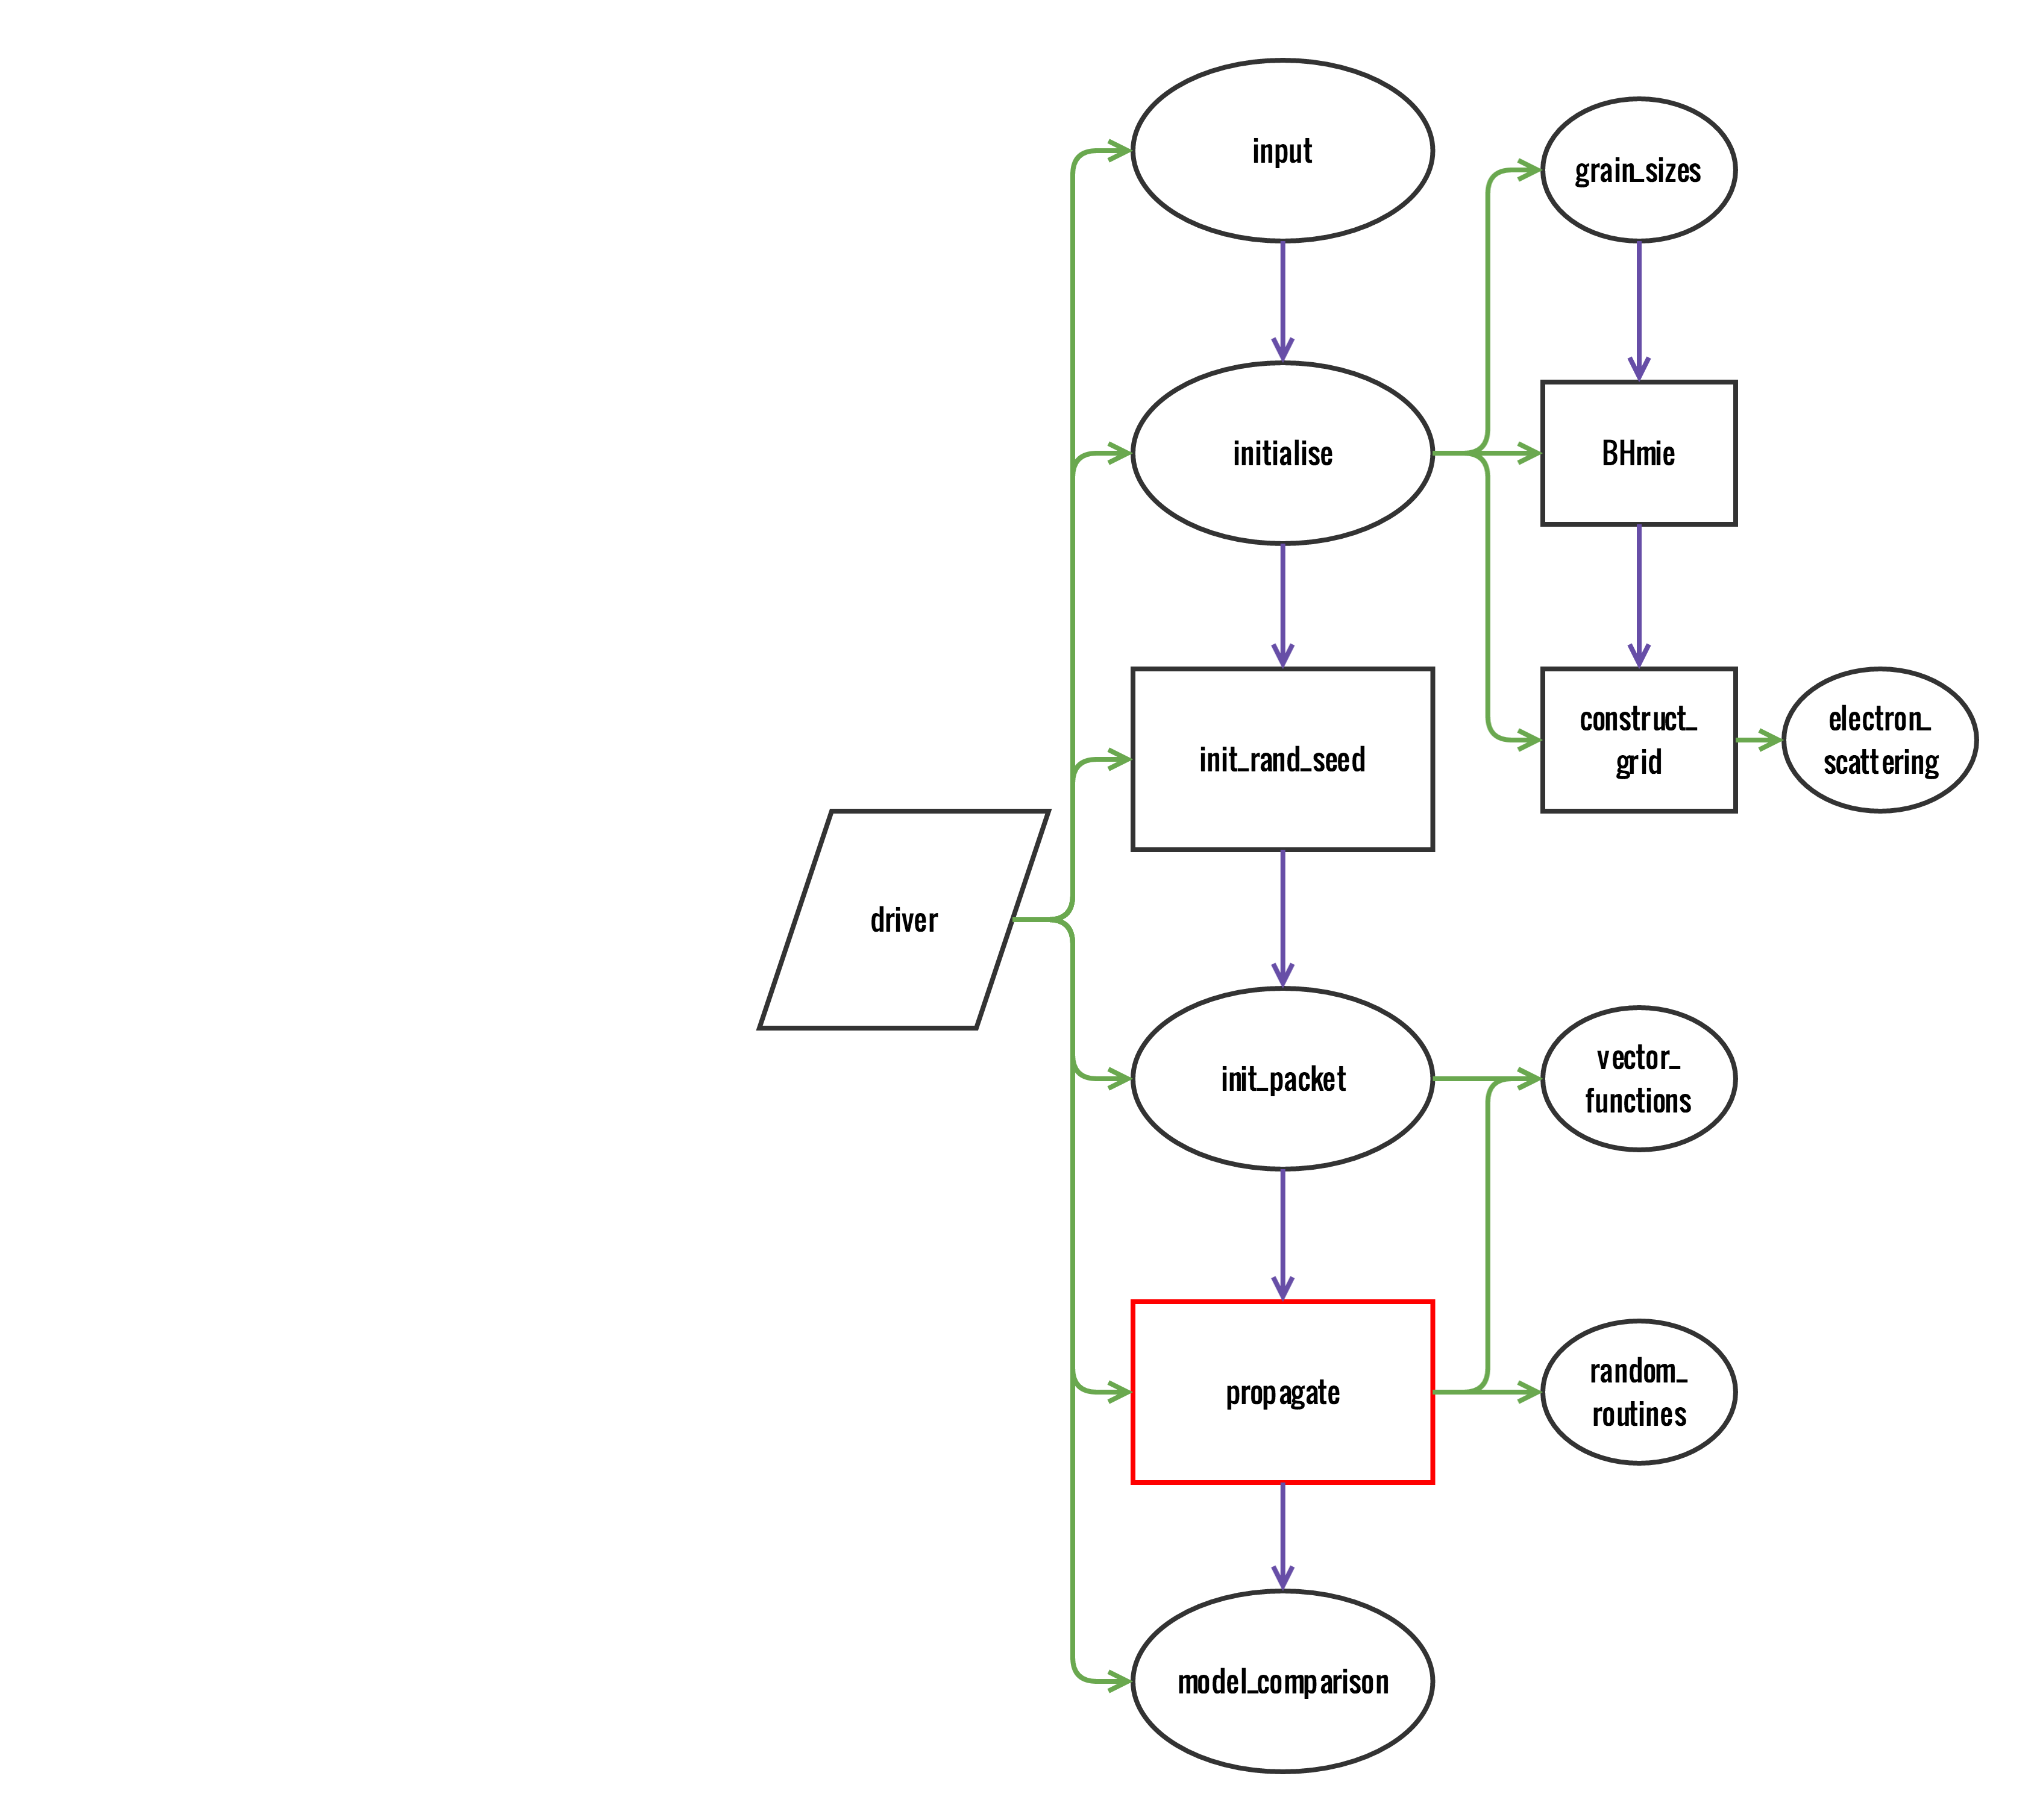
\includegraphics[scale=0.18, trim=430mm 20mm 30mm 25mm]{chapters/chapter2/code_modules_flowchart.png}
        \caption{A flowchart representing the hierarchy of modules and subroutines in the DAMOCLES code.  Ellipses represent modules and rectangles represent subroutines (the red rectangle is a recursive subroutine).  Green arrows indicate the dependence of a module or subroutine on previous modules or subroutines.  Purple arrows indicate the flow of the code.}
        \label{fig:flowchart_mods}
        \end{figure}

        
        \subsubsection{(b) The input module}
        The \textit{input} module is where the primary input file is read into the code and all global variables are declared and assigned.  A number of logicals are assigned based on values declared in the input file and some simple calculations are performed that determine the inner and outer radii based on the maximum velocity specified and the epoch of consideration ($R_{out} = V_{max} \times t$).  A number of physical constants that are used throughout the code are also declared here as ``parameters", meaning that their value cannot be changed at any point in the simulation.
        
        \subsubsection{(c) The initialisation module}
        The \textit{initialise} module acts as a driver to run all of the subroutines associated with initialising the program.  A number of dynamically allocatable arrays are declared allowing for a grid of densities to be calculated, a frequency grid to be stored and optical properties to be read in.  Arrays to store the emergent spectrum are also declared.  The calculation of dust opacities, which calls the \textit{grain\_sizes} subroutine and the \textit{BHmie} subroutine, is performed here.  For each species, the wavelength-dependent optical properties, $n$ and $k$, are read in and the Mie routine applied to every pair of frequencies and grain radii.  The resulting extinction and scattering efficiencies are summed over all grain radii for each wavelength, weighted appropriately, to calculate overall wavelength-dependent extinction and scattering opacities (see Section \ref{scn:grainsize} for further detail).  These data are stored in an array that is accessed as necessary when packets are propagated through the grid.   
        
        The command to construct the grid is called before some basic statistics about the grid are calculated.  The average optical depth from $R_{in}$ to $R_{out}$ in both the V band and the rest-frame wavelength of the line being modelled are calculated and sent to stdout.  The average number density of grains in each cell is also computed and output.  Finally, the frequency array is constructed.
        
        This module is also where the `gridcell' derived type is declared.  A `gridcell' type was specified as it allowed for easy and clear access to any of a grid cell's properties as a packet passed through it.  The type consists of a number of arrays of real, integer and logical variables.  The properties recorded for each cell include the physical bounds of the cell in each axis, the mass and number dust densities,  the electron density, an identifying number (ID) and a logical clumped property. 
        
        \subsubsection{(d) The grain size module}
        The \textit{grain\_sizes} module reads in the file that specifies the list of species to be used.  This file is a list of species detailing the name of the file containing the optical data for the species, the relative abundance of that species, the maximum and minimum grain radii and the exponent of the power law of the grain radius distribution.  It also declares how fine the grid of grain radii should be.  These properties are all read in by the \textit{grain\_sizes} module and a relative weight for each grain radius for each species is calculated here.
        
        The `species' derived type is declared in this module.  Similarly to the `gridcell' type, using a derived type allowed for the easy storing and accessing of a large number of properties of each species.  Many multi-dimensional arrays and scalars are stored for the `species' type including properties relating to the grain radius distribution, the density of a dust grain, the extinction and scatting opacities and the relative abundance of the species amongst others.  After the processing of the optical data for all species is completed, the calculated quantities are stored in arrays as components of the `species' type. 
        
        \subsubsection{(e) The Mie approximation subroutine}
		The \textit{BHmie} subroutine is a standard routine that  was obtained from an online library of routines \citep{Press2007}.  It is a modified version of the \citet{Bohren1983} Mie scattering routine.  The algorithm applies the mathematics described in Section \ref{scn:mie_theory} to determine the extinction and scattering efficiencies of a single size spherical grain at a specified wavelength given its complex refractive index $n+ik$.
		
		\subsubsection{(f) The grid construction subroutine}
		The \textit{construct\_grid} subroutine is called from within the initialisation module.  The purpose of this subroutine is to populate the grid, which is an array of derived type \textit{gridcell} and size $n_{cells}$ where $n_{cells}$ is the number of cells in the grid.   The bounds of the grid are initialised and the radii of all cells from the centre of the grid to the centre of the cell are calculated.  The density of each cell is then calculated according to a smooth power-law density distribution and scaled so that the total dust mass is equal to that specified in the input file.  If clumps are used then the total number of clumps is calculated and these are distributed throughout the grid stochastically according to the smooth density profile stipulated.
		This subroutine also calls the electron scattering subroutine contained within the \textit{electron\_scattering} module so that the electron density of a cell may be stored at the same point as the dust density.
		
		\subsubsection{(g) The electron scattering module}
		The \textit{electron\_scattering} subroutine is a simple subroutine that is used to calculate the value of $K$ as described in equation \ref{eqn:es_distn}.  The total H$\alpha$ luminosity and the gas temperature are read in and the gas temperature used to determine the appropriate value of $q_{H\alpha}$ from Table \ref{tb:q}.  These values are then used to calculate the value of $K$ as described by equations \ref{eqn:kcalc1} and \ref{eqn:kcalc2}.  The variable is passed back to the \textit{grid construction} subroutine where it is used to calculate the electron density in each cell.  The electron densities will be used by the \textit{propagate} subroutine to calculate the electron scattering optical depth in each cell.
		
		\subsubsection{(h) The random seed subroutine}
		The \textit{init\_rand\_seed} is a short subroutine that calculates a seed for the standard Fortran pseudo-random number generator (\textit{random\_number}).  It uses the system clock to generate the random seed and thus varies with every implementation of the code.  A seed is a number that is used as a ``starting point" for a pseudo-random number generator.  Varying the random seed ensures that a different set of random numbers is generated every time the code is run, which can be useful to ensure that any peculiar or interesting features of the outputted line profiles are definitely a product of the physical processes involved and not a result of random fluctuations in the simulation.  The more packets are used however, the more the Monte Carlo noise in the emergent line profile is reduced and the contribution from any anomalous packets should be insignificant.
		
		\subsubsection{(i) The packet initialisation module}
		The \textit{init\_packet} module is responsible for the creation and emission of packets at the start of the simulation.  It is called from the driver for each packet.  By generating an array of five random numbers, the position and emission direction vectors in the rest frame of the emitter are calculated according to the formulae described in equations \ref{eqn:isotropic} to \ref{eqn:isotropic3}.  The scalar velocity of the emitter is calculated based on its radial position and this converted into a velocity vector by normalising the position vector and multiplying by the scalar velocity.  The velocity vector is passed to the Lorentz transforms subroutine contained in the \textit{vector\_functions}  module.  The frequency of the packet is also passed to this subroutine.  After the propagation direction vector and the frequency of the packet have been updated to the observer's rest frame, the grid cell in which the packet starts its path is identified and the code passes back to the driver to propagate the packet through the nebula.
		
		\subsubsection{(j) The vector functions module}
		A number of vector functions are contained within the \textit{vector\_functions} module and are accessed throughout the program.  These include normalisation functions, conversions from spherical coordinates to cartesian and both forward and inverse Lorentz transforms.  It is the latter of these that are most important for the physics of the code.  The Lorentz functions are called for each packet at emission from the \textit{driver} and at every subsequent scattering event from within the \textit{propagate} routine.  As well as performing the necessary frequency shift based on the velocity of the scatterer or emitter, they also transform into and out of the rest frame of the particle thus ensuring that the packet is propagated through the nebula with a direction in the rest frame of the observer but that its new direction is sampled from an isotropic distribution in the rest frame of the emitting or scattering dust grain.  
		
		The $\beta$ and $\gamma$ values are calculated based on the input velocity vector.  The momentum 4-vector $\boldsymbol{P}$ is then multiplied by the Lorentz matrix $\boldsymbol{\Lambda}$ using the Fortran function \textit{matmul} to produce a  new frequency and a new direction vector in the appropriate frame of reference.  If a scattering event has occurred then the weight of the packet is also updated here.  The new direction vector, frequency and weight are then passed back to the propagate routine and the process repeated.   At each scattering event the inverse Lorentz matrix must first be applied to move from the observer's rest frame to the particle's.  A new direction vector must then be sampled from an isotropic distribution before applying the forward Lorentz transform to move back from the rest frame of the dust grain to the observer's frame.  The next step in the packet's trajectory may then be calculated in the \textit{propagate} subroutine.
		
		\subsubsection{(k) The propagate subroutine}
		The \textit{propagate} subroutine is at the heart of the Monte Carlo simulation.  It is here that the trajectories of all packets in the simulation are determined.  The \textit{propagate} subroutine is a subprogram called a recursive subroutine.  This allows the subroutine to call itself, at which point it will loop back to the start of the subroutine.  It will continue this process until a condition is reached that instructs it to return to the driver.  In this case a number of conditions will arrest the circulation of the packet. If the packet has escaped the outer radius of the ejecta or has been absorbed then the routine will pass this information along with the frequency and weight of the packet back to the driver.  The routine would also stop recurring if a packet has undergone a maximum number of scattering events (500 by default).  At this point it is deemed that the weight of the packet is so small as to be negligible and it is classified as ``inactive".  This prevents the code from lagging by becoming stuck on a particular packet that has become trapped in a region of high density and albedo. It is noted that if this is the case for a large number of packets then a bias may be introduced - packets emitted in particularly high density regions may be discarded more frequently than those emitted in less dense regions.  The number of packets that are deemed ``inactive" is output as a percentage of the total number of packets employed at the start of the simulation as a check for the user.  In practice, unless the albedo of the dusty medium is extremely high and the medium is very dense, this is rarely an issue (for an average simulation with $10^7$ packets, normally only one or two are discarded for this reason). 
				
		\begin{centering}
		\begin{figure}
		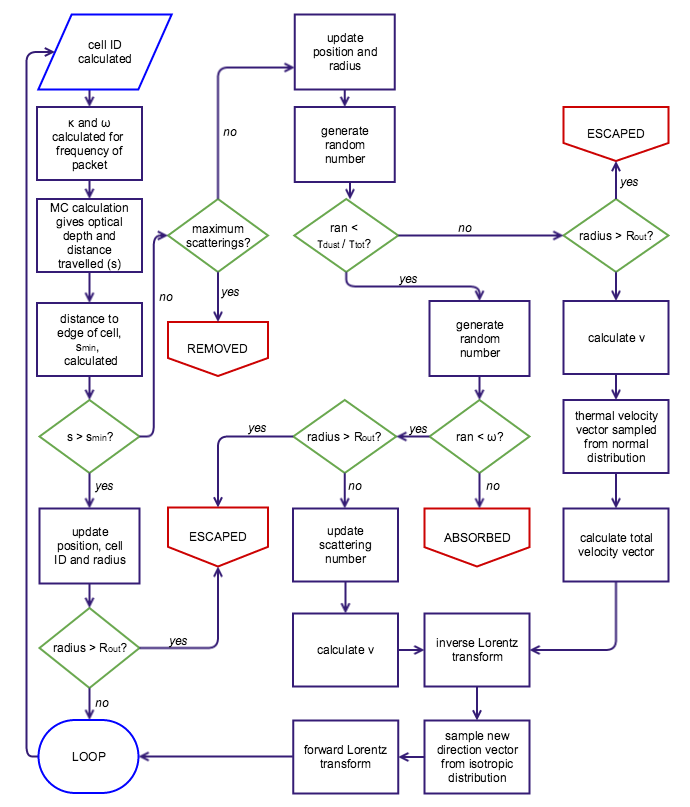
\includegraphics[scale=0.165, trim=1180mm -20mm 28mm -20mm]{chapters/chapter2/propagate_module.png}
		\caption[A flowchart representing the processes that occur in the \textit{propagate} subroutine]{A flowchart representing the processes that occur in the \textit{propagate} subroutine.  The life of a packet passing through the grid may be determined by following the flowchart starting at the blue parallelogram (top left).  Purple rectangles indicate a standard step in the evolution, green diamonds indicate that a determination must be made, red boxes mean that the packet's evolution has concluded as it has escaped, been absorbed or been removed and the blue oval indicates a return to the start of the routine.}
		\label{fig:flowchart_propagate}
		\end{figure}
		\end{centering}
		
		There are a number of processes that take place in this module in order to propagate a packet through the nebula accurately.  A full pictorial representation of the procedures that are implemented in this module may be found in the flowchart in Figure \ref{fig:flowchart_propagate}. For each packet in each grid cell, the optical depth in that cell is calculated based on the dust density and the opacity at the wavelength of the current packet.  These are obtained by interpolating between discrete opacities at points in the frequency array.  At this stage, the Monte Carlo technique is applied in order to determine the distance travelled by the packet by sampling from the cumulative probability distribution.  This displacement is then compared to the distance from the packet's current location to the edges of the grid cell in order to ascertain whether or not the packet escapes the cell.  If it does escape then the packet advances to the bounds of the current grid cell and the process is repeated in the next cell.  If it does not escape then an event occurs.  In this case, random numbers are sampled in order to determine whether the packet experiences electron scattering, dust scattering or absorption.  If the packet is absorbed then it is removed from the simulation, the \textit{propagate} subroutine is arrested and the code returns to the driver to emit a new packet.  If it is scattered then the velocity vector is calculated.  In the case of electron scattering this involves considering the thermal velocity component as well as the bulk velocity at that radius.  The Lorentz transforms are applied based on the velocity vector and the frequency and weight of the packet are updated.  A new direction of propagation is sampled in the scatterer's rest frame from an isotropic distribution and is transformed into the observer's rest frame.  The routine is recalled to start afresh with the new propagation direction. 
		
		\subsubsection{(l) The random routines module}
		The \textit{random\_routines} module contains a single subroutine which is, like the \textit{BHmie} routine, a standard routine obtained from an online library.  It allows for a random velocity vector to be sampled from a normal distribution with specified mean and standard deviation.  The standard deviation is calculated as per equation \ref{eqn:sigma_maxwell} and passed to the subroutine which samples a random 3-dimensional vector from the normal distribution with the specified standard distribution and zero mean.  This is passed back to the \textit{propagate} routine where it is added to the bulk velocity in order to determine the overall velocity of the scattering electron.
		
		\subsubsection{(m) The model comparison module}
		The \textit{model\_comparison} module is responsible for post-processing the outputted line profile and comparing the model results with inputted observed data.  The routine interpolates between two model frequency points to obtain a flux value at each frequency point of the observed line profile.  Both profiles are then normalised such that the total flux is unity.  A MSE calculation is then performed as per equation \ref{eqn:chi2}. The smaller the value of MSE, the better the fit is.  It should be noted however that observational data with a poor signal-to-noise ratio will have an inherently larger MSE than data with a good signal-to-noise ratio.
		
		
		\subsection{OpenMP Parallelisation}	
		\label{scn:open_mp}
		
	Monte Carlo simulations are exceptionally well-suited to parallelisation.  The path of each packet through the nebula is unaffected by the transport of any other packet.  It is therefore possible to run multiple instances of the \textit{propagate} module at once by using several threads.  Since the vast majority of the processing power of the simulation is driven from this module, it is theoretically possible to achieve a nearly linear speed-up; i.e. if the number of cores is doubled, the run time should be approximately halved.  %check for threads, cores or processors? 
	
	DAMOCLES was parallelised using OpenMP.  OpenMP is an Application Program Interface (API) that allows for shared-memory parallel programming in Fortran and C/C++.  OpenMP causes the code to be run serially on a single processor until a parallel region is reached.  At this point the single master thread branches into multiple threads, and multiple instances of the same section of code are run on each.  In DAMOCLES, this splitting occurs at the start of the loop which controls the emission and propagation of packets from each shell.  If, for example, $10^7$ packets are emitted and 5 threads are used, then approximately $2 \times 10^6$ packets will be independently processed on each thread.  Practically however, the OpenMP keyword \textit{dynamic} is declared ensuring that, as soon as each thread has finished processing a packet, it immediately moves onto the next one.  If the \textit{static} keyword were specified instead then the number of packets to be processed would be equally divided between the threads at the start of the loop.  In this case, if, by random chance, one thread happened to have significantly more absorbed packets than another, then potentially utilisable processing power would be lost as the core waited for the others to finish.
	
	At the start of the parallel region variables accessed within the shared region are specified as shared or private.  Private variables are not seen by other threads and allow the value of a single named variable, for example ``frequency", to have different values on different threads.  Shared variables have the same value regardless of the thread number, for example, ``grid cell density".  As each packet escapes, its weighted energy must be added to the final energy array.  It is important that two threads do not attempt to alter the value of this shared array at the same time as data may be lost or corrupted. This section of code is therefore enclosed inside a \textit{critical} region.  This instruction ensures that code in this block is to be executed by only one thread at a time.  Extensive testing was performed to ensure that outcomes were not affected by the implementation of a parallel environment.
	
	For further information about the OpenMP API please refer to \citet{Chapman2007}.
	
	\subsection{Input Variables}
	
	There are a significant number of parameters that may be varied in the code.  Many of these are important variable parameters that will be the parameters of interest when modelling.  However, there are also a significant number of variables that allow other properties of the model to be controlled.  All parameters can, broadly,  be divided into one of three categories:  properties of the emitted rest-frame line or doublet, properties of the dust and gas in the ejecta and properties of the grid and code architecture.  I list all the variables that are input in the primary input file in Table \ref{tbl:input} and will here briefly describe the basic meaning and function of each one.
	
	\begin{table}[htdp]
	\caption{The input variables read in from the input file and example values}
	\begin{center}
	\def\arraystretch{1.5}
	\begin{tabular}{l r c c l r}
	\toprule
	Input Variable & Example Value &&& Input Variable & Example Value\\
	\midrule
	lambda1\_0 & 636.3 &&& MD\_tot & 1.0e-4\\
	L\_tot & 0.003 &&& l & 1.0\\
	L\_Halpha & 0.005 &&& q & 1.3\\
	doublet & 1 &&& b & 2.0\\
	lambda2\_0 & 630.0 &&& gas\_shell & 1\\
	L\_ratio & 3.1&&& v\_max\_gas & 8000\\
	ES & 1 &&& Rrat\_gas & 0.05\\
	ES\_temp & 10000 &&& l\_gas & 1.0\\
	LS & 0 &&& q\_gas & 1.5\\
	VelShift & 1 &&& b\_gas & 2.0\\
	MF & 0.5 &&& ncells & 50\\
	FF & 0.1 &&& n\_packets & 1e8\\
	dayno & 680 &&& n\_bins & 1000\\
	v\_max & 5000 &&& n\_shells & 100\\
	Rrat & 0.2 &&& dustfile & ``species\_file.in"\\
	\bottomrule
	\end{tabular}
	\end{center}
	\label{tbl:input}
\end{table}%

\vspace{0.8cm}

\subsubsubsection{(a) Properties of the emitted rest-frame line or doublet}
\subsubsubsection{lambda1\_0 }  

This is a real number that specifies the initial rest-frame monochromatic wavelength at which packets are emitted in nanometres.  If a doublet is to be modelled then this represents the wavelength of one of the singlets.

\subsubsubsection{L\_tot }

L\_tot is the total luminosity of the line in units of $10^{40}$ ergs s$^{-1}$.  The initial energy of each packet ($E_0$) is therefore L\_tot divided by the total number of packets used in the simulation (n\_packets). For lines which have flux calibrated observed spectra, this allows the flux of the line to be modelled in addition to the normalised shape.  This variable is also used to estimate the undepleted luminosity of the observed line when it is initially emitted from the ejecta.

\subsubsubsection{L\_Halpha}

Similar to L\_tot, L\_Halpha is the total luminosity of the H${\alpha}$ line.  In the case of H${\alpha}$ modelling, this value should be the same at the value of L\_tot.  This variable is used in the calculation of the electron density and it is not necessary to specify it unless the electron scattering environment is switched on (see section \ref{scn:ES} for further details).  

\subsubsubsection{doublet}

This is an integer of value 1 or 0 that indicates the use or otherwise of the doublet environment.  If set to 1 it triggers the doublet logical in the code to be initialised to \textit{true}.  The code will then read in the values of {lambda2\_0} and {L\_ratio} in order to initialise packets with two different starting monochromatic wavelengths.  Packets are processed through the nebula as normal before being collated in bins weighted according to both their history and the intrinsic flux ratio of their parent singlet.

\subsubsubsection{lambda2\_0}

This is a real number that specifies the initial rest-frame monochromatic wavelength of packets emitted from the second line in a doublet environment.  The wavelength is specified in nanometres.

\subsubsubsection{L\_ratio}

This real number gives the ratio between the respective luminosities of the lines in a doublet environment.  The ratio should be declared as the flux at lambda1\_0 divided by the flux at lambda2\_0.  It is expected that the doublet environment will generally be used to model forbidden lines, for example the [OI]$\lambda$6300,6363\AA\ doublet, where the intrinsic flux ratio between the singlets may be theoretically determined.

\vspace{0.8cm}

\subsubsubsection{(b) Properties of the dust and gas in the ejecta}
\subsubsubsection{ES}

This keyword is similar to the doublet keyword in that, by setting it equal to 1 or 0, it indicates the use or otherwise of the electron scattering environment.  If it is set to 1 then it initialises the electron scattering logical in the code to \textit{true}.  If the electron scattering environment is switched on then this triggers the calculation of electron densities for every cell in the grid.  This density contributes to the total optical depth of a cell and, as packets are propagated through each cell, they will experience an electron scattering event with probability $1-e^{\tau_e}$, where $\tau_e$ is the electron scattering optical depth.

\subsubsubsection{ES\_temp}

 When the electron scattering environment is switched on, it is necessary to calculate the electron density of each cell in the grid.  In order to do this an average gas temperature must be specified to allow for $q_{H\alpha}$ to be determined.  DAMOCLES will not accept any value for this input variable; only 5,000K, 10,000K and 20,000K will be accepted.  These are thought to be a representative range of temperatures for the ejecta of supernovae at epochs where electron scattering still has the potential to influence observed line profiles.  These specific values were selected since they are the values of $q_{H\alpha}$ that are given in \citet{Osterbrock2006}.

 \subsubsubsection{MF}

 If this keyword (short for mass fraction) is set to 0 then a smooth density distribution of both gas and dust will be constructed.   If it is not however, then this will automatically initialise the clumping logical present in the code to \textit{true}.  The value specified should be between 0 and 1 and gives the total fraction of the dust mass that should be located in clumps.  The remaining fraction will be smoothly distributed according to the power-law density profiles declared in the input file.

 \subsubsubsection{FF}

 If the clumping environment is switched on (using the \textbf{MF} keyword) then \textbf{FF} declares the total filling factor of the clumps.  The filling factor is defined as the fraction of the total volume of the ejecta that is occupied by clumps.  For a fixed clump size, this parameter effectively determines the number of clumps to be used.  Once the number of clumps to be used has been determined, the mass fraction then determines the density of the clumps.
 
 \subsubsubsection{dayno}

 This keyword represents the epoch being modelled.  In combination with the declared maximum velocity, it is used to consistently calculate an outer radius as 
 \begin{equation}
 R_{out}=8.64 \times 10^{-6} \Big( \frac{t}{\mathrm{days}} \Big) \Big( \frac{v_{max}}{\mathrm{kms^{-1}}} \Big)
 \label{eqn:Rout_calcn}
 \end{equation}

 \noindent where $R_{out}$ is in units of $10^{15}$cm.

 \subsubsubsection{v\_max}

 This is the maximum velocity used in the code.  It is assumed to be the velocity at the outer radius of the ejecta and is used to construct a velocity profile of the form
 \begin{equation}
 v(r) = v_{max} \Big( \frac{r}{R_{out}} \Big)^l
 \label{eqn:vel_law}
 \end{equation}

 where $l$ is also declared in the input file and $R_{out}$ is calculated based on the epoch and the maximum velocity.

 \subsubsubsection{Rrat}

 This number is the ratio between the inner and outer radii.  Once the outer radius has been calculated as per Equation \ref{eqn:Rout_calcn}, this ratio is used to calculate the value of the inner radius.

 \subsubsubsection{MD\_tot }

 This real number specifies the total dust mass to be distributed throughout the grid in solar masses ($M_{\odot}$).

 \subsubsubsection{l}

 $l$ is the exponent of the radial velocity law in the code as per equation \ref{eqn:vel_law}.

 \subsubsubsection{q}

 $q$ describes the relationship between the radial dust density distribution and the emissivity distribution.  It is the exponent of the emissivity distribution as a function of density such that $i(\rho) \propto \rho^q$ where $i(\rho)$ is the emissivity at a given density.  Though this parameter may take any real value, it is frequently fixed to be $i(\rho) \propto \rho^2$, i.e. proportional to the product of the recombining proton and electron densities in the case of H$\alpha$ and to the product of the neutral atom oxygen and electron densities in the case of collisionally excited emission (e.g. [O~{\sc i}], [O~{\sc iii}]).


 \subsubsubsection{b}

 This parameter describes the value of the exponent of the dust density distribution in terms of radius such that $\rho \propto r^{-b}$.

 \subsubsubsection{gas\_shell}

 This flag may be set to 0 or 1 to indicate that dust and gas are coupled or decoupled respectively.  If it is set to 1 then the ``decoupled" logical in the code is set to \textit{true} and the gas follows a density distribution that is independent of the density distribution followed by the dust.  The following five parameters specify the geometry of the emitting gas.  It is worth noting that in the case where gas and dust are coupled to each other, the gas follows the same distributions as specified for dust by the parameters described above. 

 \subsubsubsection{v\_max\_gas}

 This is the gas analogue of the v\_max parameter described above.  

 \subsubsubsection{Rrat\_gas}

 This is the gas analogue of the Rrat parameter described above.  

 \subsubsubsection{l\_gas}

 This is the gas analogue of the parameter $l$ described above.  

 \subsubsubsection{q\_gas}

 This is the gas analogue of the parameter $q$ described above.  

 \subsubsubsection{b\_gas}

 This is the gas analogue of the parameter $b$ described above.  

\vspace{0.8cm}

 \subsubsubsection{(c) Properties of the grid and code architecture}
 \subsubsubsection{LS}

 For an initially symmetric distribution of gas and dust, it is not necessary to specify a line of sight as all lines of sight will produce the same profile.  It is therefore more efficient to collect all packets that escape regardless of their direction of flight.  However, if an alternative, axisymmetrical or asymmetrical geometry is adopted then the ability to specify a line of sight is important.  If this keyword is set to 1 then the ``line of sight" logical will be initialised as \textit{true}.  Only packets that escape within a cone of vertical angle $\pi/6$ will be collected.  Clearly, in practice, the angle would be very much smaller but it is prohibitively expensive to run enough packets through the simulation that enough are collected to achieve a reasonable resolution when a very small  angle is adopted.  A representation of this construction is presented in Figure \ref{fig:LOS}.

 
 \begin{figure}
 \centering
 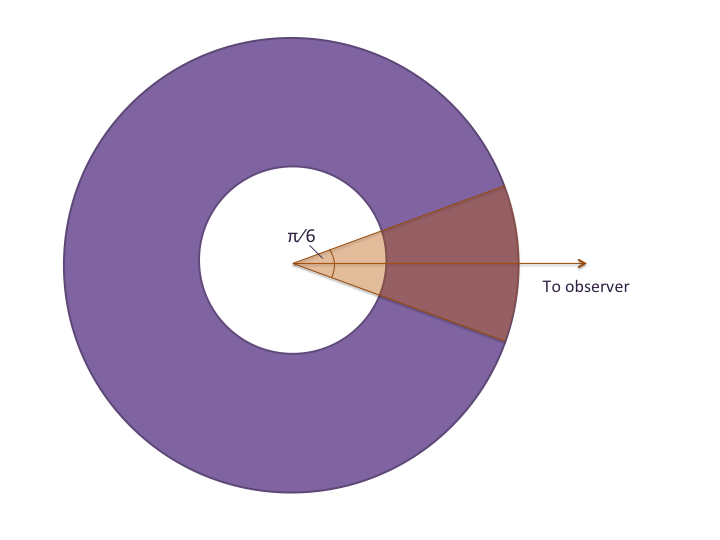
\includegraphics[scale=0.55, trim=-25mm 10mm 29mm 0mm]{chapters/chapter2/LoS_diagram.png}
 \caption{Schematic representing which packets are collected when the line of sight environment is switched on.  Packets that contribute to the emergent line profile are those that escape the nebula within a cone with vertical angle $\pi/6$.}
 \label{fig:LOS}
 \end{figure}
 
 \subsubsubsection{VelShift}

 This is another environment flag.  As a packet is transported through the nebula it may experience repeated scattering events that shift its original frequency beyond that expected from the maximum theoretical velocity.  It is discused in depth in the next chapter how this process of ``velocity shifting" may result in a profile that exhibits an extended red wing.  It is useful for the purposes of comparison and investigation to be able to turn off this process of repeated scattering events so that the only frequency shift experienced by a packet is at the initial emission.



 \subsubsubsection{ncells}

 Each axis is split into this number of divisions.  The total number of cells in the grid is therefore ncells$^3$.


 \subsubsubsection{n\_packets}

 This variable determines the number of packets to be emitted and processed through the grid.  This parameter is particularly important for achieving a resolution that is high enough to give representative results.  The larger the number of packets used, the less noise is present in the final profile.  The Monte Carlo process introduces noise that can sometimes be construed as a result when it is in fact a numerical artefact.  Using a large number of packets reduces this risk and improves the output of the model.  In general, the more dense an environment, the more packets it is necessary to use.  This is because any packets which are absorbed are removed from the simulation and therefore reduce the desired resolution.  Since the vast majority of the total processing power is used to propagate packets through the grid, an increase in the number of packets results in a significant reduction in runtime. Optically thick simulations of dust with a very high or a very low albedo have a significantly longer runtime than optically thin scenarios.  When choosing this parameter, a careful balance must be found between the total runtime and the desired resolution. 


 \subsubsubsection{n\_bins}

 This value gives the total number of divisions in the frequency array and thus determines the overall frequency resolution of the output line profile.  Since the resulting profile is in fact a histogram binned into a frequency array, it is important that these divisions are fine enough to provide a seemingly continuous line profile.  Apparent jumps or discontinuities could be produced if too few bins are used.

 \subsubsubsection{n\_shells}

 This parameter controls the total number of shells the ejecta is divided into at the start.  If a particularly steep radial profile is adopted for either the velocity profile or the density profile then the user may wish to increase the number of shells used to compensate.  Increasing the number of shells will have an effect on the overall runtime, but this will be insignificant in comparison to altering the number of packets.  

 \subsubsubsection{dustfile}

 Finally, this string gives the name of the input file that itemises the list of dust species, their relative abundances and size distributions.

 \begin{table}
 \caption{List of all outputs and example values produced by the DAMOCLES code.}
 \begin{center}
 \def\arraystretch{1.5}
 \begin{tabular}{ l  r}
 \toprule
 Output & Example Value \\
 \midrule
 Total number of cells      & 125000 \\
 Number of grid cells inside ejecta   & 65544 \\
 Total volume of supernova ejecta (10$^{42}$ cm$^3$)   & 304523264 \\
 Volume of a grid cell or volume of a clump (10$^{42}$ cm$^3$)   & 4668.52\\
 Width of a grid cell (cm) &   1.67e+15\\
 \midrule
 Mass check (calculated as $\rho V$)   & 6.03e-04 \\
 \midrule
 Average grain number density (cm$^{-3}$)  & 1.96e-09\\
 $C_{ext}$ at rest-frame wavelength  & 2.94e-08 \\
 $C_{sca}$ at rest-frame wavelength  & 1.63e-08 \\
 Albedo at rest-frame wavelength & 0.554 \\
 Average optical depth to rest-frame wavelength  & 2.062 \\
 Average optical depth in V band  & 2.18 \\
 \midrule
 Average electron density (cm$^{-3}$) & 71509.1 \\
 Average electron scattering optical depth &   1.31e-02\\
 \midrule
 Total number of packets      &          100000\\
 Number of active (propagated) packets      &          100000\\
 Number of inactive packets        &            0\\
 Number of absorbed packets      &          82949   \\
 Percentage of absorbed packets out of all active packets & 82.95 \\
 Number of packets in line of sight  & 17050       \\
 Percentage of escaped packets in line of sight & 100.0 \\
 \midrule
 Estimated undepleted line luminosity ($10^{40}$ ergs s$^{-1}$)  & 1.10e-05\\
 Total (depleted) luminosity ($10^{40}$ ergs s$^{-1}$) & 1.90e-06\\
 Total energy absorbed ($10^{40}$ ergs s$^{-1}$) &  1.57e-06\\
 Energy per active packet ($10^{40}$ ergs s$^{-1}$) & 1.90e-11\\
 \midrule
 MSE	& 0.3557  \\
 \bottomrule
 \end{tabular}
 \end{center}
 \label{tb:outputs}
\end{table}%

\subsection{Output, Post-Processing and Visualisation}

The primary output file contains details of the emergent line profile.  Three columns are written out to the file at the end of the simulation.  These are the wavelength, velocity and flux of the modelled line profile.  Another output file is also produced by the \textit{model\_comparison} module.  This file prints both the inputted observed line profile and the outputted emergent line profile to one file in the same velocity bins.  This allows for easy plotting.  The columns printed in  this file are wavelength, modelled flux and observed flux. The total flux is normalised to unity for both line profiles.  Both of these files may be represented graphically in a straightforward fashion using any plotting package.  In addition to these output files, a number of useful quantities are also calculated by DAMOCLES and output to \textit{stdout} throughout the course of the simulation.  If desired, the user may direct the \textit{stdout} to a file for a record of these quantities.  A list of all quantities output by DAMOCLES is given in Table \ref{tb:outputs}.

Throughout my modelling, I used standard and custom routines written with MATLAB to plot line profiles, both modelled and observed.  I also use MATLAB to process some of the data.  For example, where I have observations with accurate observed fluxes, I scale the modelled profile to the observed profile so that fluxes remain to scale.  This is initially performed by a custom MATLAB routine which smooths the modelled data to reduce any Monte Carlo noise before identifying the maximum flux value.  Identifying the peak flux of the observed line profile allows the modelled profile to be automatically scaled.  Any inaccuracies in the scaling may then be easily adjusted manually.  I also use MATLAB for any other illustrative graphs or plots, for example, the plots in Figure \ref{fig:grid} were generated in MATLAB using its 3D-scatter plotting function.

\section{Further Developments}
\label{limitations}

The modular structure of DAMOCLES allows for easy implementation of additional functionality in the future.  By simply adding extra modules, extra physics can be included in the code.  There is potential for this code to be expanded in a number of directions.  An immediately apparent development involves the dust itself.  The treatment and understanding of the dust in the ejecta is crucial to understanding the shape of the line profile.  The ability to place different species in different locations within the ejecta is not currently included.  This would allow for stratified or asymmetrical distributions of dust species motivated by the potentially discrete locations of the parent elements.  Similarly, streamlining the ability to model arbitrary density distributions and geometries would allow for more complex and accurate modelling of supernova ejecta.  The ejecta of SN~1987A, for example, is known to have an asymmetric distribution which could potentially affect the contour of the line profile (e.g. \citet{Sinnott2013}).

As mentioned previously, dust grains are rarely perfectly spherical and can be far more complicated in shape.  It might be of interest to include a module that treats a continuous distribution of ellipsoids  \citep{Bohren1983}, as mentioned in Section \ref{scn:dust_med}, in order to more accurately model the effects of different dust grain shapes.
%More widely, supernova explosions can sometimes result in radiation that is polarised.  By including the capacity to model polarised radiation in the code, we may able to glean further information about the distribution and nature of dust forming within the ejecta.
%
Subsequent development of the code has allowed for the consideration of the effects of modelling forward scattering.  By adopting the Henyey-Greenstein model, forward scattering was included for a fixed value of the anisotropy parameter $g$ \citep{Henyey1941}.  Resultant line profiles were affected only slightly, with profiles exhibiting a reduced degree of both absorption and scattering due to a lower incidence of scattering events.  However, because of the spherically symmetric geometry of the models and the original isotropic emission, the observed effects of including forward scattering were found not to be substantial even for an extremely high value value of $g = 0.98$.  Further development of the code should allow for arbitrary phase functions to be implemented and the treatment of anisotropic scattering should be included by default where non-spherically symmetric geometries are modelled.  In these cases, the effects of forward scattering may be more significant than in cases of spherically symmetric geometries.  Anisotropic expansion of supernova ejecta can sometimes result in radiation that is polarised.  By extending this development to include the capacity to model polarised radiation, we may be able to glean further information about the distribution and nature of dust forming within the ejecta.  

It would also be theoretically possible to expand the code to become a fully self-consistent radiative transfer code or to include certain approximations (e.g. the Sobolev approximation) to allow for full spectral modelling of non-optically thin lines throughout the optical and infrared.

Aside from the development of the code directly, the current process of manual fitting can be laborious and has the potential miss potentially good fits due to the large number of variable parameters.  I have completed some work over the course of this PhD wrapping DAMOCLES in a MCMC (nested sampling) routine that allows for a more thorough investigation of parameter space resulting in a full multivariate probability distribution.  For reasons of time, the research presented in the following chapters was performed using manual fitting but further work finishing the implementation of this routine or a similar one would be invaluable in the future.






%\clearthesisemptydoublepage
%\chapter{Benchmarking and Sensitivity Analyses}\label{chp:chp3}

\begin{flushright}
  {\em QUOTE GOES HERE }\\

\ \

\normalsize
{AUTHOR}  
\end{flushright}

\section{Introduction}
\section{Analytical Results}
\section{Optically Thin Line Profiles}
\section{Optically  Thick Line Profiles}
\section{Sensitivity Analyses}
	\subsection{Dust Mass}
	\subsection{Velocity Profile}
	\subsection{Density Profile}
	\subsection{Grain Size Distribution}
	\subsection{Electron Scattering}
	\subsection{Ratio of Inner and Outer Radii}
	\subsection{Dust Species}
	%\subsection{Doublets}
\section{Conclusions}

\noindent{FIRST PARAGRAPH}

THE REST FOLLOW HERE. 



\clearthesisemptydoublepage


%\begin{flushright}
%  {\em QUOTE GOES HERE }\\
%
%\ \
%
%\normalsize
%{AUTHOR}  
%\end{flushright}
\chapter{Probing DAMOCLES:  Testing and a Parameter Sensitivity Analysis}\label{chp:chp4}

The introduction of any new piece of software into a field has the potential to yield exciting new results.  The first step in this process should therefore be a thorough investigation into the reliability of the code and an assessment of the outputs from a theoretical standpoint.  Before the modelling of real data takes place, it is important to understand why the variation of a  given parameter affects results in a particular way.  A comprehensive understanding of parameter space not only facilitates the modelling process but may also give rise to interesting results in and of itself.

To this end, this chapter describes the ways in which DAMOCLES was tested and the results of these tests.  I then also present a parameter sensitivity analysis.  I describe the changes that are seen in the shapes of line profiles and consider any distinctive features that arise as a result of varying the parameters of interest.  I also consider the physical processes behind these effects.


\section{Testing and benchmarking the code}

The field of astronomy is highly reliant on the production of bespoke software to understand and interpret observations from telescopes and to develop and test new theories.  As one of only a few sciences which do not have the ability to run experiments or to validate results in a laboratory, progress is made via mathematical analyses or computational models based on observed data.  Astrophysicists typically develop their own programs because a deep understanding of the topic to be modelled is required.  Like any experiment, however, the ``apparatus" should be checked and tested in order to establish its reliability.

Throughout the production of DAMOCLES, I sought, as far as was possible, to maintain best practices in scientific computing as detailed by \citet{Wilson2012}.  The code is carefully structured into modules and subroutines as described in the previous chapter.  Each of these units was inspected for sense and accuracy as it was written, and at each update and addition the code as a whole was tested against basic logical checks, for example comparing outputs to manually calculated properties.  I used GitHub for version control and uploaded new versions after any significant alterations.  In addition to regular evaluations conducted throughout the program development, it was very important to establish that DAMOCLES produced standard results as expected.

There is a general lack of published models in the literature that consider dust-affected asymmetric line profiles.  This is problematic since there are no published benchmark cases against which I could compare results.  I therefore considered a number of analytic line profiles derived from first principles for the case of a dust-free spherically symmetric expanding medium.  This process ensured the functionality of the grid and the initialisation and propagation of energy packets.  Additionally, I also checked the the absorption and scattering components of the code which are crucial to the modelling of a dusty medium.  I  considered some optically thick scenarios and qualitatively compared my results with those presented by \citet{Lucy1989}.  The profiles presented by  \citet{Lucy1989} were produced both analytically and from numerical modelling and are of scenarios that are typical of those treated by DAMOCLES.  They are also the only published numerical models of dust-affected asymmetric line profiles and as such it is important that DAMOCLES is capable of reproducing these results.

\subsection{Theoretical line profiles from first principles}
\label{analytics}

The simple nature of a spherically-symmetric expanding medium with a given velocity outflow law and emissivity distribution allows for analytical line profiles to be calculated from first principles in the dust-free case.  Based on the methods of \cite{Gerasimovic1933},  I derive a set of three equations that describe the contours of theoretical line profiles under different starting conditions.



Describing the fractional expansion velocity of the shell as $v(r) \propto 
r^\alpha$ with $\alpha \neq 0$ such that $v(r)=\frac{V(r)}{V_{max}}$ where 
$V(r)$ and $V_{max}$ represent physical velocities and $v_{max}=1$, the velocity along the line-of-sight to the observer is given by 
\begin{equation}
\label{eqn:radial_vel}
u(r,\theta)=r^\alpha \cos \theta
\end{equation}

\noindent where $r=R/R_{max}$ is the fractional radius and $R$ and $R_{max}$ represent physical radii. For curves with constant line-of-sight velocity $u=const$ we therefore have
\begin{equation}
\,d r = \frac{r}{\alpha} \tan \theta \,d \theta
\end{equation}

\begin{figure}
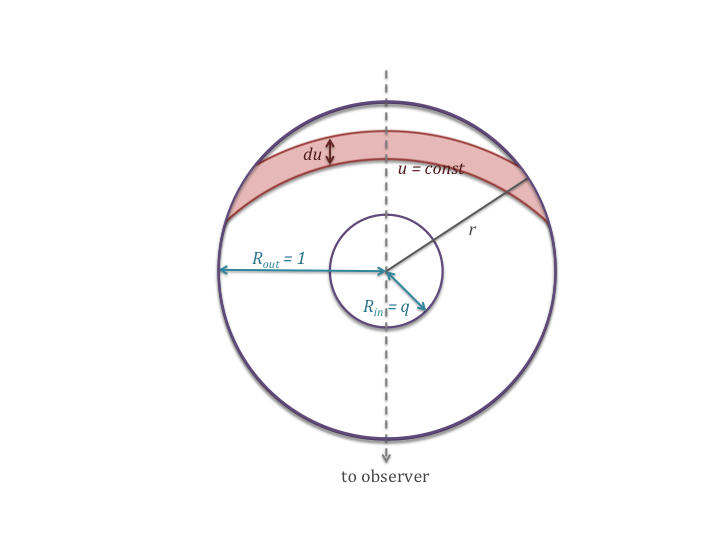
\includegraphics[clip=true,scale=0.5,trim= 180 50 130 70]{chapters/chapter4/images/opt_thin_diag/curve.png}
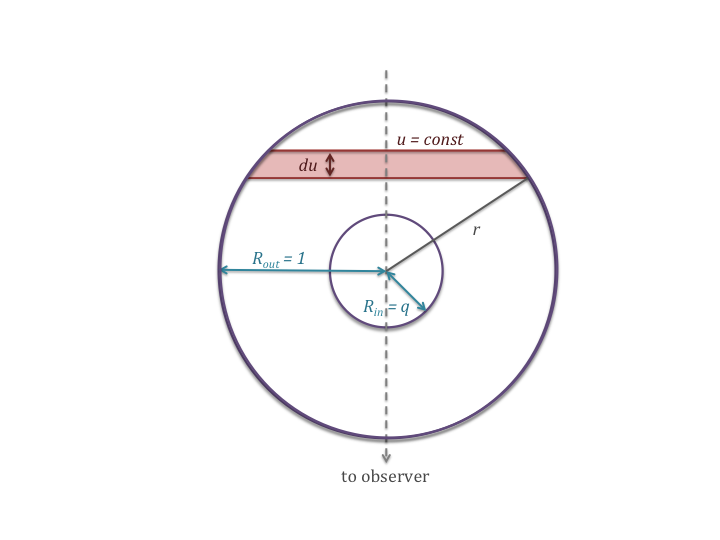
\includegraphics[clip=true,scale=0.5,trim= 180 50 130 70]{chapters/chapter4/images/opt_thin_diag/line.png}
\caption{Diagrams illustrating the dust-free model and some of the relevant variables used in the derivation of the equations of analytical line profiles.  On the left is the general case with curves of constant $u$ labelled.  On the right is the special case of an orthogonal $(u,s)$ net when $\alpha=1$ and therefore $v(r) \propto r$.}
\label{fig:analytics}
\end{figure}


\noindent For $u=const$, the line element $\, ds$  is given by
\begin{equation}
\label{eqn:ds}
\, ds^2 = r^2 \, d\theta^2 + \, dr^2 = r^2 \Big( \frac{\tan^2\theta}{\alpha^2}+1 \Big)\, d\theta^2
\end{equation}

\noindent and therefore, along curves of constant $u$ we have
 \begin{equation}
 \label{eqn:vs}
s = u^{\frac{1}{\alpha}} \int_{\theta_{0}}^{\theta_{1}} \frac{\sqrt{\frac{\tan^2\theta}{\alpha^2}+1}}{\cos ^ {\frac{1}{\alpha}}\theta}\, d\theta
\end{equation}


\noindent The angle $\psi$ between the tangent to a curve and the radial line  is given by the formula (in polar coordinates) \begin{equation}
\tan \psi = r \frac{\, d \theta}{\, d r} 
\end{equation}

\noindent which for curves of $u=const$ gives
\begin{equation}
\tan \psi = \frac{\alpha}{\tan \theta}
\end{equation}

Curves of constant line-of-sight velocity therefore intersect the line $\theta = 0$ orthogonally, although the $(u,s)$ net is only orthogonal if $\alpha=1$ (see Figure \ref{fig:analytics}).

We can now construct a volume element between $u$ and $u+\, du$ by rotating a section of thickness $\, du$  around the $\theta =0 $ axis.  Assuming that $i(r)$ is the emission per unit volume (dependent only on radius), then the energy emitted by the nebula between $u$ and $u+du$ is proportional to
\begin{equation}
\label{eqn:integral}
\int_{\mathcal{C}} \ i(r) \ r \sin \theta \ r \, d\theta \, dr  \ = \ \int_{\mathcal{C'}} \ [i(r) \ r^2 \sin \theta] \ \frac{\partial (r,\theta)}{\partial (u,s)}  \, ds \, du
\end{equation}

where the integral is a line integral along curves $\mathcal{C}$ of constant $u$ and square brackets denote a change of variables.  

We therefore compute the Jacobian from Equations \ref{eqn:radial_vel} and \ref{eqn:vs} as
\begin{equation}
\label{eqn:jacob}
\frac{\partial (u,s)}{\partial (r,\theta)} \ = \ \alpha  u \sqrt{\frac{\tan^2\theta}{\alpha^2}+1}
\end{equation}

Assuming an initial emissivity distribution dependent on radius only, we put $i(r) \propto r^{-2\beta}$ (i.e. appropriate for a gas density distribution $\rho \propto r^{-\beta}$ with the emissivity proportional to the gas density squared).  Substituting Equation \ref{eqn:jacob} into Equation \ref{eqn:ds} and calculating the curvilinear integral along curves of constant $u$ yields the following:
\begin{equation}
i(u) \,d u \ \sim \, du \int_\mathcal{C} \frac{r^{2(1-\beta)}\sin \theta}{\alpha u \sqrt{\frac{\tan^2\theta}{\alpha^2}+1}} \, ds 
\end{equation}

Substituting in Equations \ref{eqn:radial_vel} and \ref{eqn:integral} and transforming to an integral in $\theta$ gives
\begin{equation}
\begin{split}
i(u) \, du &\sim \frac{du}{\alpha u^{\frac{2\beta-3+\alpha}{\alpha}}} \int^{\theta_1}_{\theta_0} \cos^{\frac{2\beta-3}{\alpha}} \theta \sin \theta \, d\theta 
\\
&\sim  \frac{du}{u^{\frac{2\beta-3+\alpha}{\alpha}}} \Bigg[\frac{\cos^{\frac{2\beta - 3 + \alpha}{\alpha}} \theta}{2\beta -3 + \alpha}\Bigg]^{\theta_1}_{\theta_0}
\end{split}
\end{equation}

\noindent for $\frac{2\beta-3}{\alpha} \neq -1$ where $i(u) \,du$ is the energy emitted in a volume element and $\theta_0$ and $\theta_1$ are the bounds of this element.  The case $\frac{2\beta-3}{\alpha} = -1$ results in a logarithmic relationship.

\begin{figure}
\begin{subfigure}{0.5\textwidth}
\centering
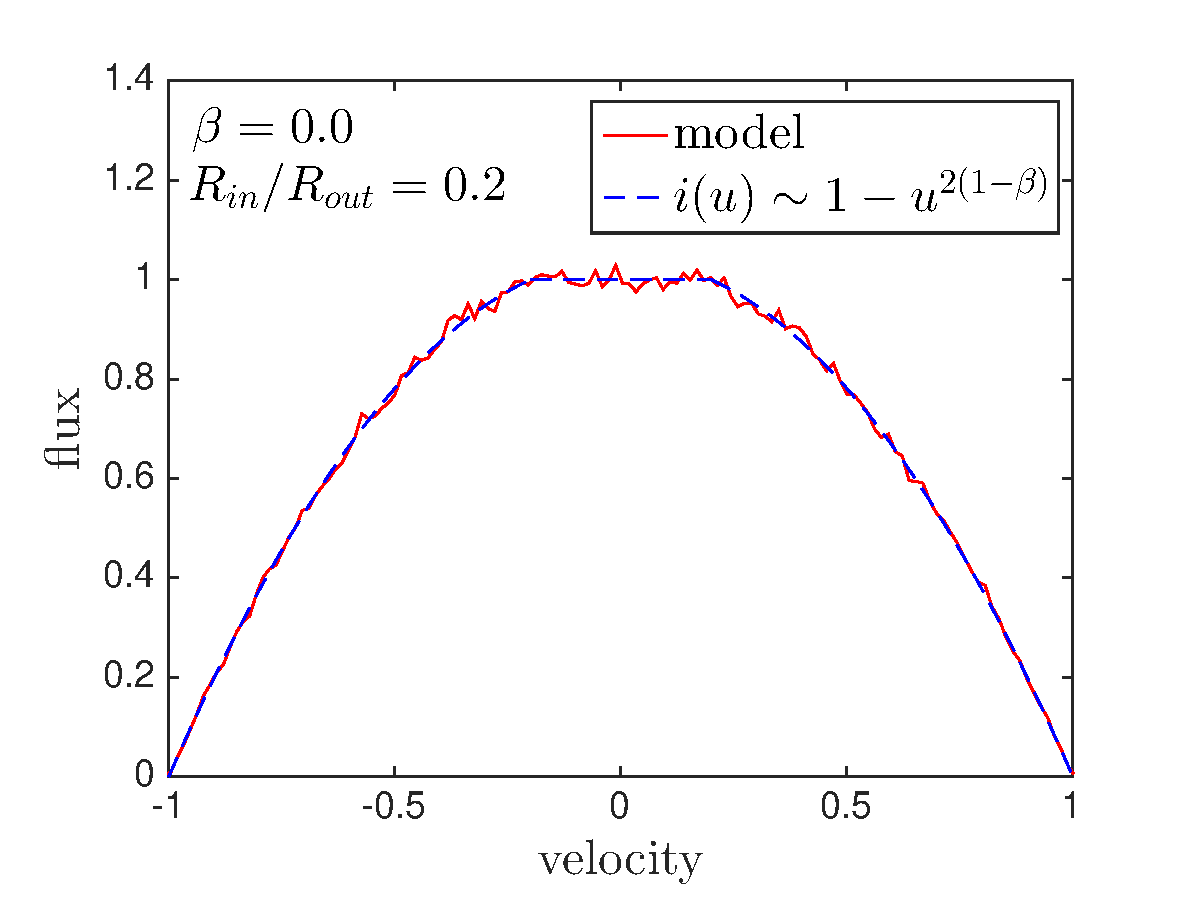
\includegraphics[trim =0 25 45 15,clip=true,scale=0.4]{chapters/chapter4/images/params/A/b0_r0_2}
\end{subfigure}
\hspace{4mm}
\begin{subfigure}{0.5\textwidth}
\centering
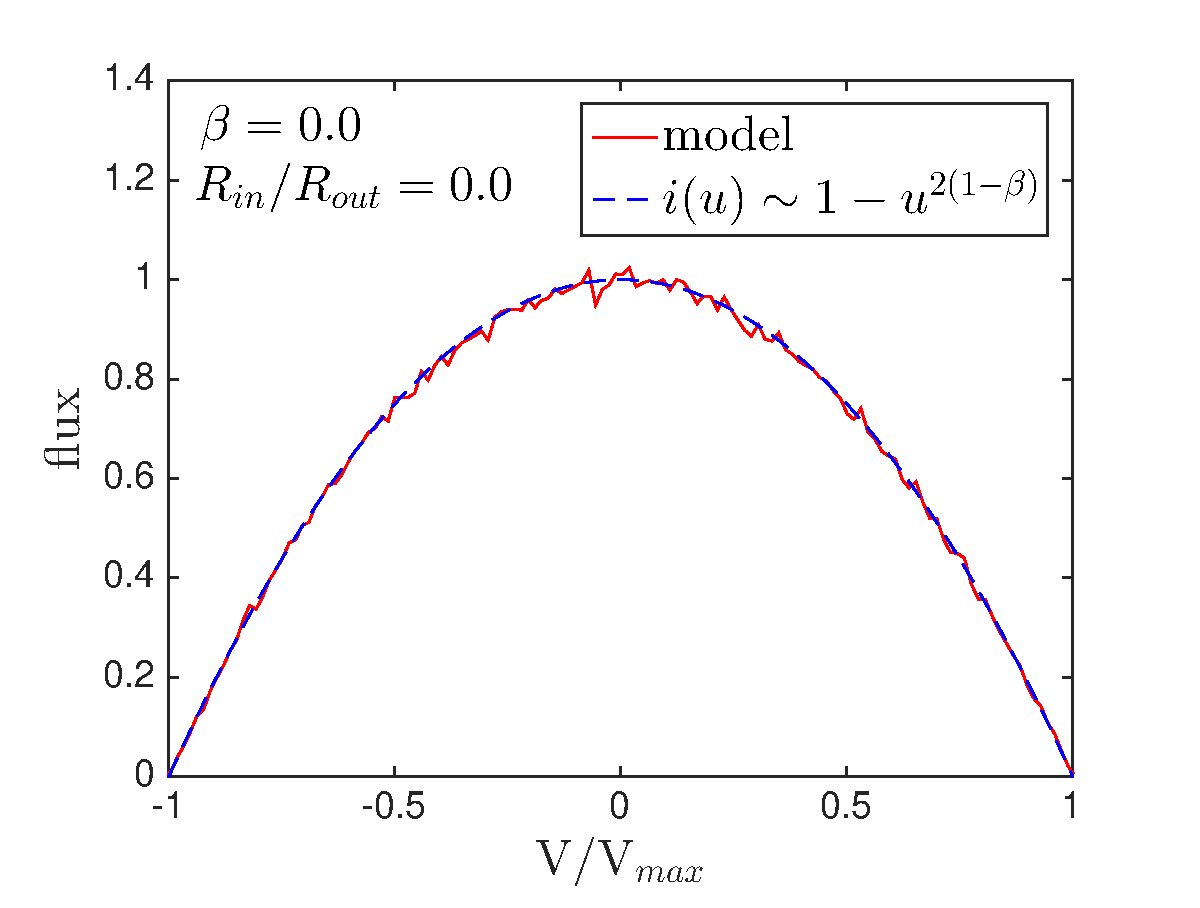
\includegraphics[trim =72 25 45 15,clip=true,scale=0.4]{chapters/chapter4/images/params/A/b0_r0}  
\end{subfigure} \\[0.0ex]

\begin{subfigure}{0.5\textwidth}
\centering
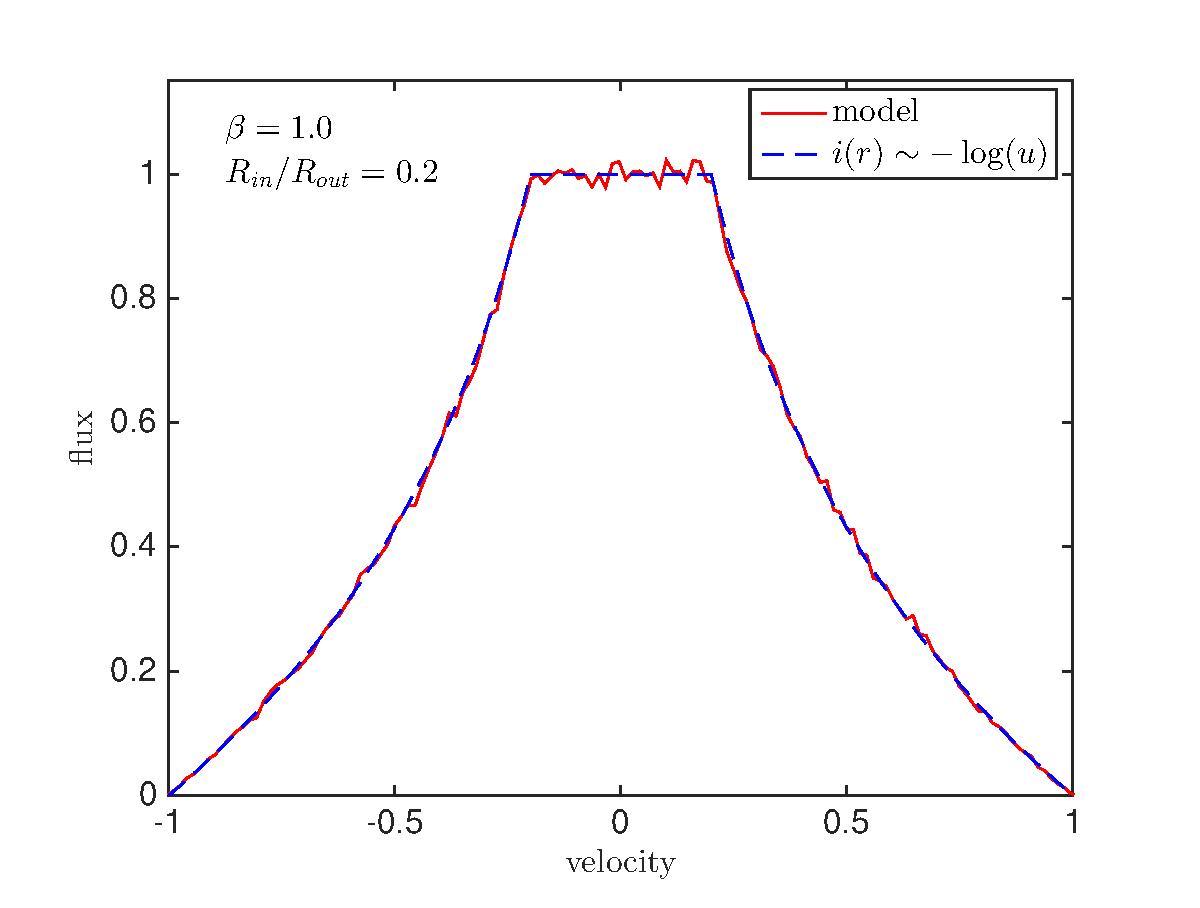
\includegraphics[trim =0 25 45 15,clip=true,scale=0.4]{chapters/chapter4/images/params/A/b1_r0_2}
\end{subfigure}
\hspace{4mm}
\begin{subfigure}{0.5\textwidth}
\centering
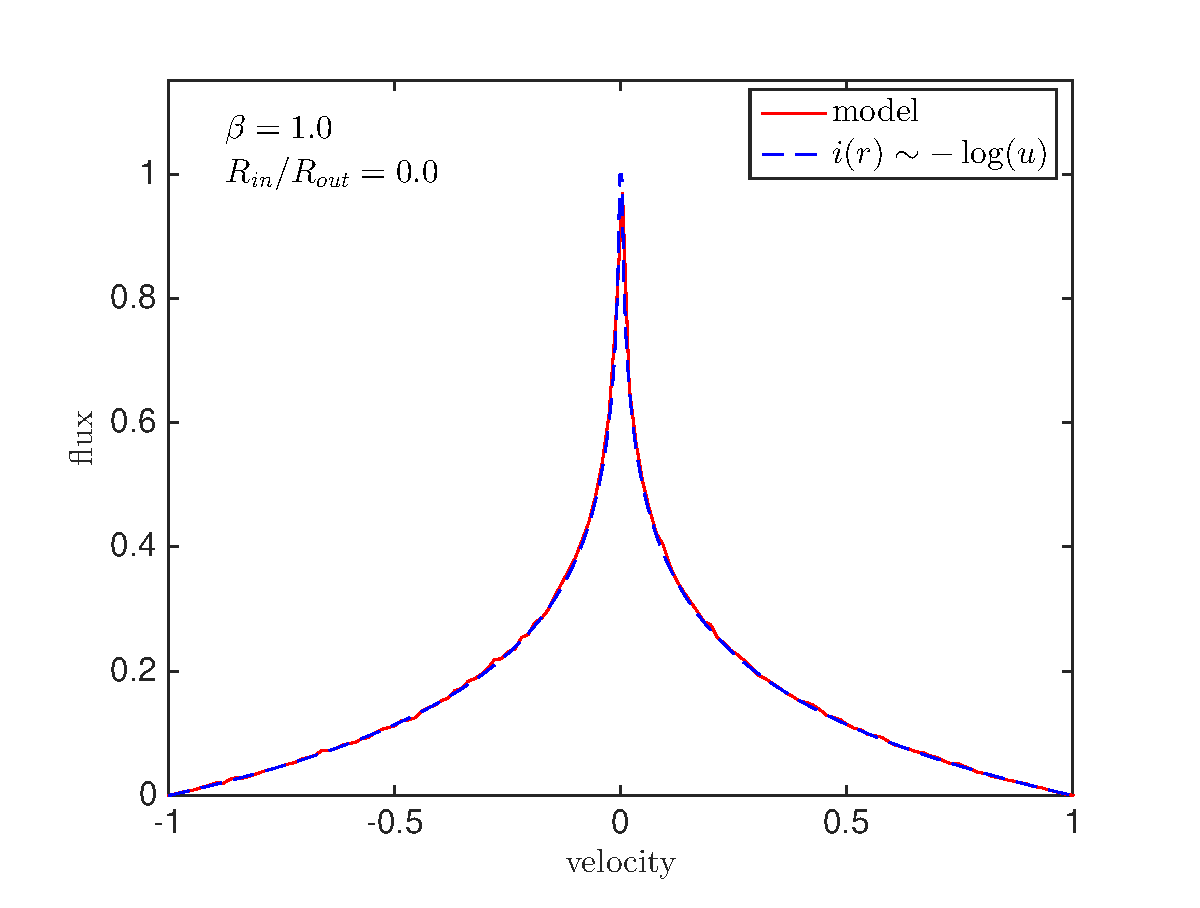
\includegraphics[trim =72 27 45 15,clip=true,scale=0.4]{chapters/chapter4/images/params/A/b1_r0} 
\end{subfigure} \\[1.0ex]

\begin{subfigure}{0.5\textwidth}
\centering
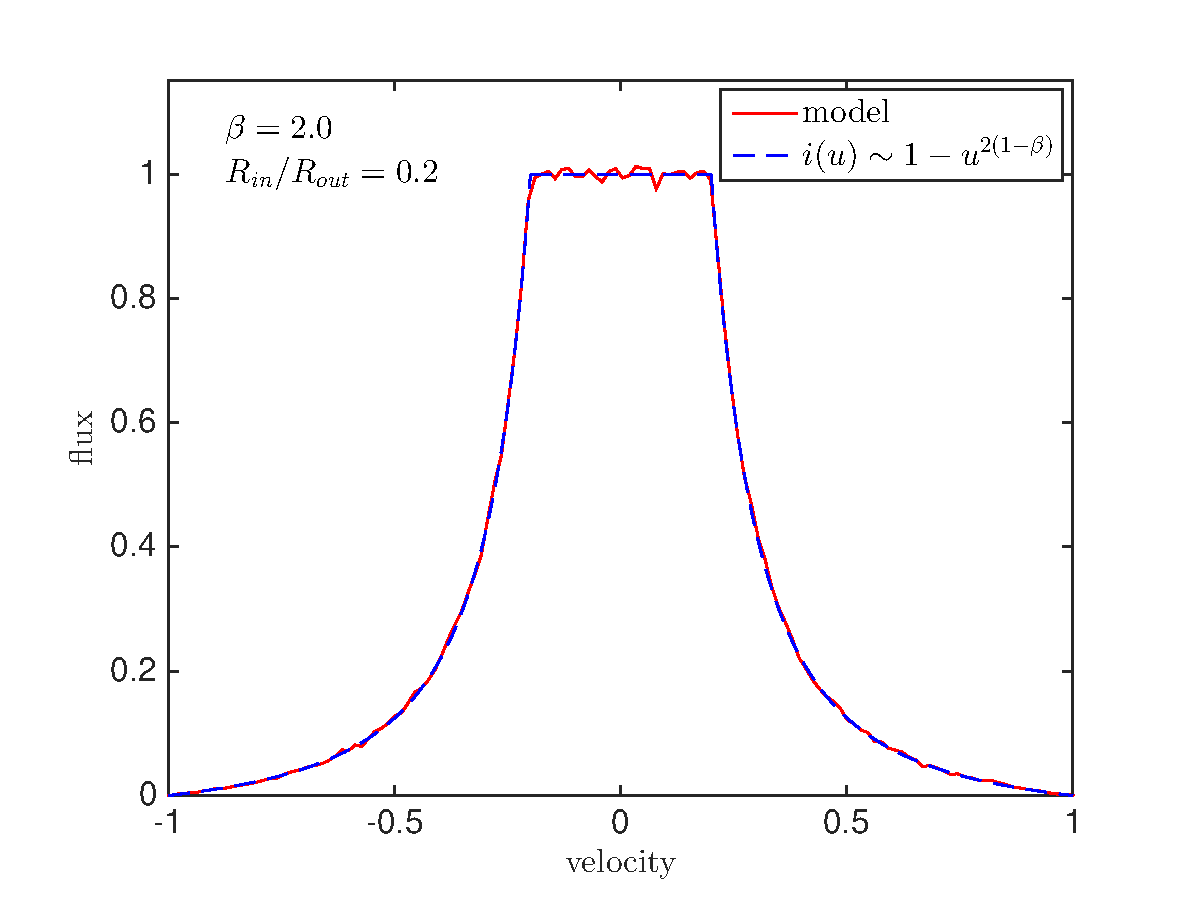
\includegraphics[trim =0 0 45 15,clip=true,scale=0.4]{chapters/chapter4/images/params/A/b2_r0_2}
\end{subfigure}
\hspace{4mm}
\begin{subfigure}{0.5\textwidth}
\centering
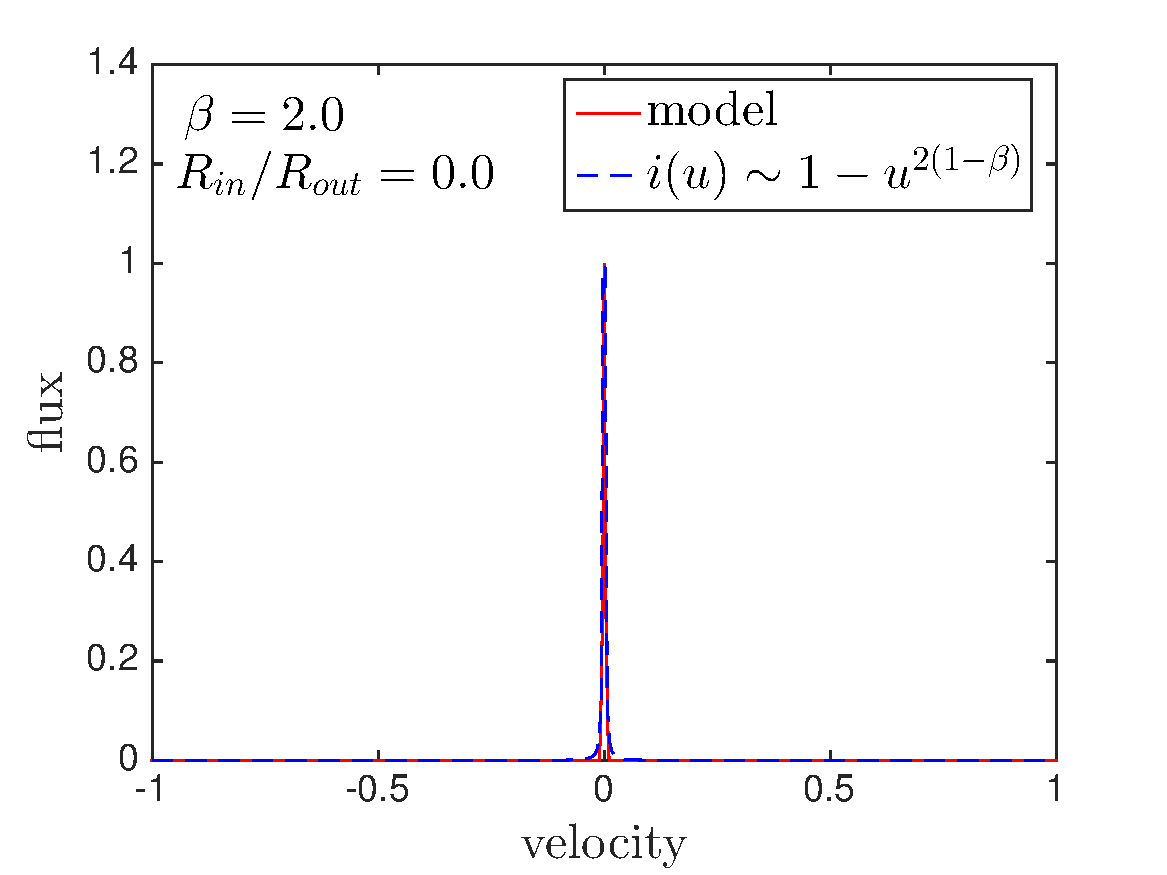
\includegraphics[trim =72 0 45 15,clip=true,scale=0.4]{chapters/chapter4/images/params/A/b2_r0.pdf}
\end{subfigure}

\caption{\textit{Red:} Benchmark models for optically thin ($\tau =0$) 
line profiles  with fractional velocity $v(r) \propto r$. Top to bottom: initial emissivity 
profiles $i(r) \propto r^{-2\beta}$ with $\beta=0.0$, $\beta=1.0$ and 
$\beta=2.0$. Cases with $R_{in}/R_{out}=0.2$ are on the left and 
$R_{in}/R_{out}=0.0$ on the right.  The presence of a plateau in the upper plots is due to the finite inner radius (detached shell). \textit{Blue:} The analytical case 
with $i(u) \sim 1-u^{2(1-\beta)}$ except in the case of $\beta=1$ where 
$i(u) \sim -\log u$.}
\label{fig:analytics}
\end{figure}



In the case of a ``filled'' nebula, i.e. one where the inner radius is vanishingly small in comparison to the outer radius the above result may be evaluated between $\theta_0=0$ and $\theta_1=\arccos u$ and the equation of the line profile is
\begin{equation}
\label{eqn:sides}
	i(u) \, du \sim \pm \frac{du}{(2\beta-3+\alpha) u^{\frac{2\beta-1+\alpha}{\alpha}}} \Big(1-u^{\frac{2\beta-3+\alpha}{\alpha}} \Big)
\end{equation}

If the nebula is not ``filled'', that is to say, the inner radius is some fraction of the outer radius and the remnant is a detached shell  with inner radius $R_{in}=q$ and outer radius $R_{out}=1$ such that $q=\frac{R_{in}}{R_{out}}$, the 
above formula is only valid from some critical value $u'=q^{\alpha}$ to $u=1$. For $u<u'$, we obtain
\begin{equation}
i(u) \, du \sim \pm \frac{du}{(2\beta-3+\alpha)} \Big( \frac{1}{q^\alpha} - 1 \Big)
\end{equation}

\noindent and therefore the top of the line is flat while the sides are 
sloping.

Crucially, the width of the flat section is determined by 
\begin{equation}
\label{eqn:flattop}
u'=q^{\alpha}
\end{equation} 

\noindent or simply $u'=q$ in the case where $v \propto r$, whilst the shape of the profile outside of the flat-topped region is described by Equation  \ref{eqn:sides}.

Profiles with a variety of shapes may be derived from these formulae  depending on the relative values of $\alpha$ and $\beta$.  Here we consider three main families of curves:


\begin{enumerate}\parskip3pt

	\item \ \ $\quad i(u)  \sim u^{-\gamma}-1$ \quad ($\alpha>0$, $2\beta-3+\alpha>0$)
	\item \ $\quad i(u)  \sim 1-u^\gamma$ \quad \ \ ($\alpha>0$, $2\beta-3+\alpha<0$)
	\item  $\quad i(u) \sim -\log u$ \quad \ \ ($\alpha>0$, $2\beta-3+\alpha=0$)

\end{enumerate}

\begin{figure}
\centering
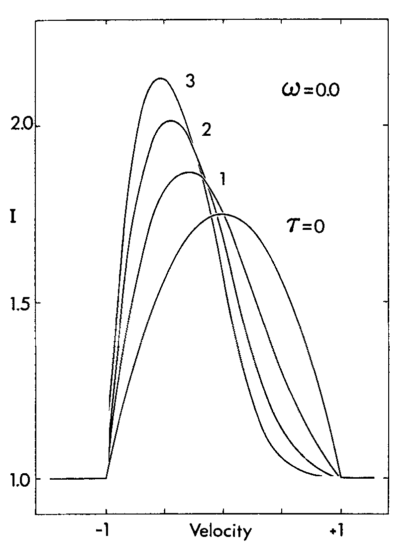
\includegraphics[trim =0 0 0 0,clip=true,scale=0.6]{chapters/chapter4/images/Lucy89_Model2.png}
\caption{The analytically derived line profiles of \citet{Lucy1989} corresponding to their Model II scenario with zero albedo dust, for a variety of total dust optical depths.}
\label{fig:LucyMod2}
\end{figure}

\noindent where $\gamma$ is defined as $\gamma= \lvert 
\frac{2\beta-3+\alpha}{\alpha} \rvert$.

Models are presented for each of these cases, both for a filled nebula and for a shell structure with $R_{in}/R_{out}=0.2$.  A velocity profile $v \propto r$ appropriate for supernova ejecta in the free expansion phase is used throughout \citep{Li1992,Xu1992,McCray1996,Baron2005}.  Values of 
$\beta = 0, 1$ and $2$ are adopted.  Figure \ref{fig:analytics} 
illustrates the excellent agreement between the analytical case and the 
models.  All fluxes are scaled to unity at the peak.

I conclude from this testing that all aspects of the code that are associated with initialising the packets into the grid are functioning correctly since an error at this stage would result in disagreement with the above theory.  

\subsection{Benchmarking against numerical models}
\label{opt_thick_testing}
\begin{figure}
\centering
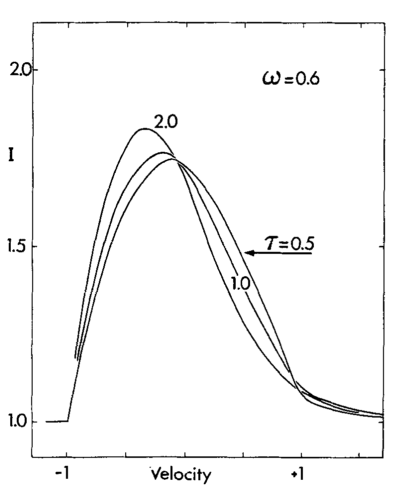
\includegraphics[trim =0 0 0 0,clip=true,scale=0.6]{chapters/chapter4/images/Lucy89_Model3.png}
\caption{The numerically modelled line profiles of \citet{Lucy1989} corresponding to their Model III scenario with dust of albedo $\omega=0.6$, for a variety of total dust optical depths.}
\label{fig:LucyMod3}
\end{figure}



In addition to the tests for the optically thin line profiles detailed above, I also compared my outputs to those derived by \citet{Lucy1989} in order to assess the accuracy of the scattering and absorption aspects of the code.  
I  considered two similar cases, equivalent to Models II and III of 
\citet{Lucy1989} (see Figures \ref{fig:LucyMod2} and \ref{fig:LucyMod3} respectively). In the first case, dust with zero albedo (pure absorption) was 
uniformly distributed throughout a filled nebula with a velocity profile 
$v \propto r$.  In the second case, the same scenario was considered but in a 
medium of dust with albedo $\omega =0.6$.

In the first case, the profile may once again be derived analytically from 
the basic geometry using the fact that radiation will be attenuated by a 
factor $e^{-2\tau_{\nu} v}$ between points with line-of-sight fractional 
velocities $-v$ and $+v$ where $\tau_{\nu}$ is the optical depth at 
frequency $\nu$ from the centre to the outer edge of the ejecta.  The line 
profile is therefore given by
\begin{equation}
\frac{I(v)}{I(-v)} = \exp(-2\tau_{\nu} v)  
\end{equation}
\begin{figure}
\begin{subfigure}{\textwidth}
\centering
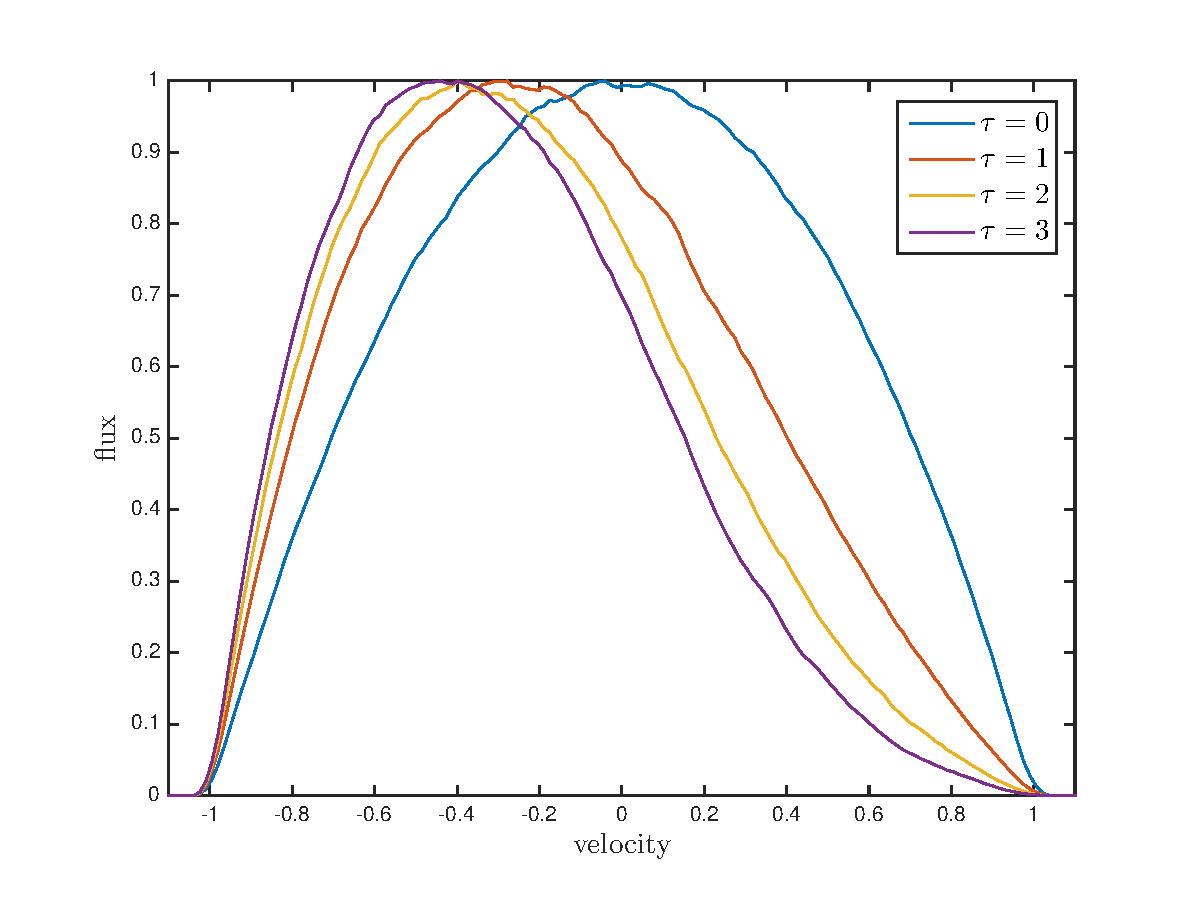
\includegraphics[trim =10 0 45 15,clip=true,scale=0.67]{chapters/chapter4/images/params/opt_thick_w0}
\end{subfigure} \\[1ex]
\begin{subfigure}{\textwidth} 
\centering
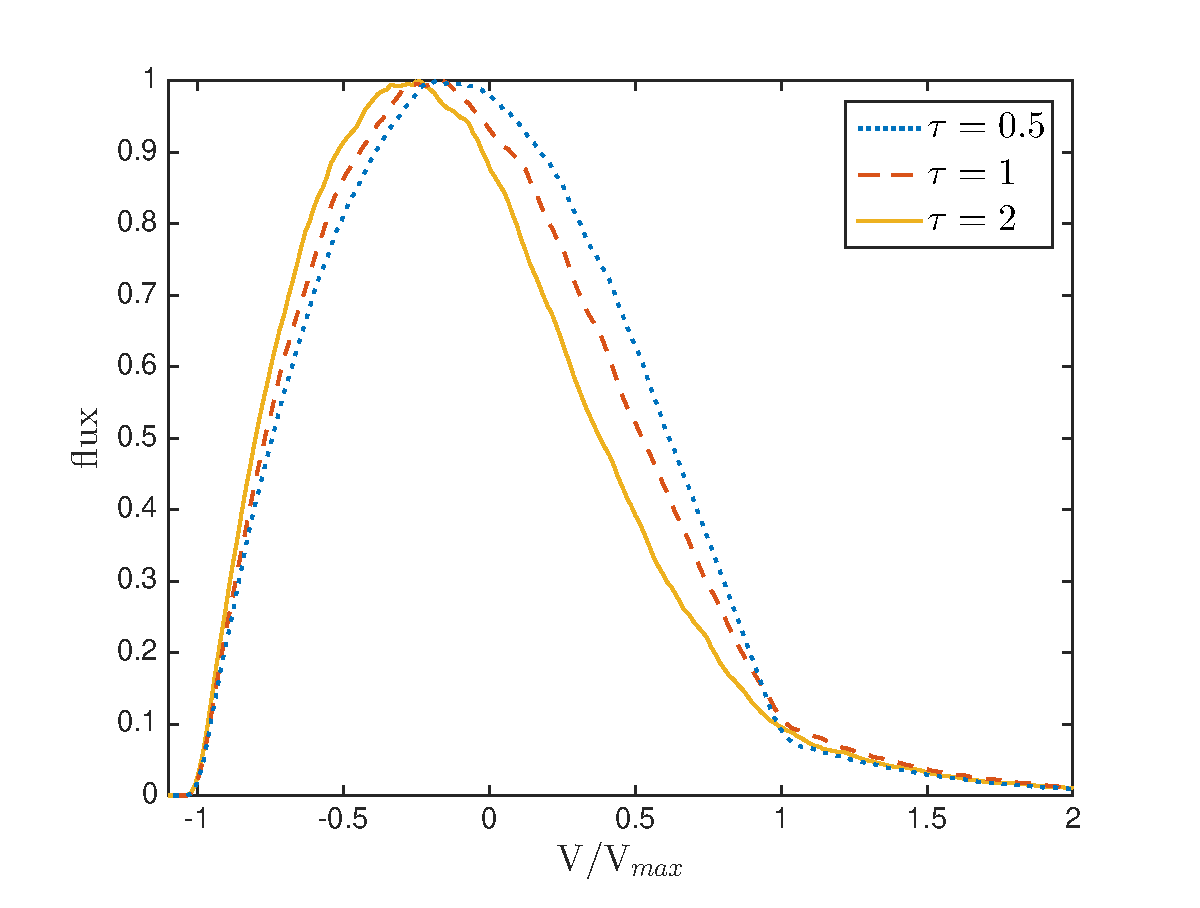
\includegraphics[trim =10 0 45 15,clip=true,scale=0.67]{chapters/chapter4/images/params/opt_thick_w0_6}
\end{subfigure}  
\caption{Benchmark models for line profiles  with $v \propto r$, $i(r) \propto$ constant and a filled sphere with $R_{in}/R_{out}=0$.  Pure dust absorption models ($\omega = 0$) are presented in the top plot, whilst partially scattering models are presented at the bottom ($\omega = 0.6$) as per \citet{Lucy1989} Models II and III. All resulting profiles have been scaled to unity flux at their peaks.}
\label{fig:Lucy}
\end{figure}


\citet{Lucy1989} presented several examples for both the analytical case of 
the perfect absorber and a Monte Carlo model for grains with albedo $\omega 
=0.6$.  I include their profiles here for comparison in Figures \ref{fig:LucyMod2} and \ref{fig:LucyMod3}.  I  present line profiles in Figure \ref{fig:Lucy} that were generated by DAMOCLES using the same model parameters as described by \citet{Lucy1989}.  I note that 
the resulting profiles exhibit the same features and shape. The peaks of all profiles are shifted further to the blue with increasing optical depth and all profiles are also flux-biased towards the blue.  Of particular 
interest is the scattering wing that appears beyond the maximum velocity 
($v_{max}=1$) on the red side of the profiles in the partial 
scatterer case as a result of the packets doing work on the expanding sphere.  
This was noted by \citet{Lucy1989} as a potential diagnostic for the 
presence of dust in the ejecta of a supernova and I  will discuss this 
further in the next section.


%\subsection{Testing the electron scattering mechanism}
%\subsection{Clumped models in smooth limits}


%%%%%%%%%%%%%%%%%%%%%%%%%%
\section{A Parameter Sensitivity Analysis}
\label{param_sens_analysis}
It is of general interest to establish potential diagnostic signatures in 
the line profiles of supernovae and their remnants in order to trace dust 
formation more effectively. The capacity to specify a number of parameters is included in DAMOCLES.  The variation of each parameter potentially affects the contour of the resulting line profile in a different way.  By investigating each parameter separately over a range of values whilst keeping the other parameters fixed, it may be possible to identify certain characteristics of dust-affected line profiles that may be associated with a particular property of the dusty medium.  This insight could help to explain unusual or interesting features of observed line profiles where dust is suspected to be an influential factor.  In this chapter, I investigate and discuss the effects of the main 
parameters of interest, namely:

\begin{itemize}
\item the maximum velocity, $V_{max}$
\item the ejecta radius ratio, $R_{in}/R_{out}$
\item the dust optical depth,  $\tau$
\item the dust albedo, $\omega$ 
\item the dust density profile exponent, $\beta$, where $\rho \propto r^{-\beta}$
\end{itemize}

I also investigate the capacity of this type of model to infer properties of the dust itself, specifically the dust grain radius range and distribution, and the variety and relative abundances of different grain species present in the dusty medium. 


\subsection{The maximum line velocity, $V_{max}$}

The maximum velocity is defined as the velocity at the outer edges of the 
line emitting region for a given line.  The maximum velocity may vary 
between different spectral lines or doublets due to different locations of 
species having differing ionization thresholds.  Clearly, the larger the 
maximum velocity used the wider the profile becomes.  To some extent 
therefore the steepness of the density profile and the maximum velocity 
can act to counter each other since a steeper density distribution narrows 
the profile (see Section \ref{beta}).  The shape of the wings of the 
profiles, however, generally precludes much degeneracy in this aspect - the 
overall shape of the line profile can be used to determine the exponent of 
the density distribution to within a relatively small range.

More important is the effect that the maximum velocity has on the overall 
optical depth.  Since the outer radius is calculated directly from the 
maximum velocity (as $R_{out}=V_{max} \times t$ where $V_{max}$ is determined from the blue side of the observed line profile), the overall volume of the ejecta is determined solely by 
this value and the ratio of the inner and outer radii.  The total dust 
optical depth to which the radiation is exposed can therefore be greatly 
affected by even a relatively small change in the maximum velocity for 
fixed values of the other parameters.  Practically, however, the maximum 
velocity can usually be fairly well determined from the observations 
(identified as the point where the flux vanishes on the blue side) and may 
be further constrained through modelling.

\subsection{The ejecta radius ratio, $R_{in}/R_{out}$}

As already discussed in Section \ref{analytics}, the width of the flat top 
is determined by the ratio of the inner and outer radii, the exponent of 
the velocity profile and the maximum velocity.  I assume that the 
supernova is in free expansion from just a few months after the explosion 
and therefore $r=vt$ such that within the ejecta the velocity profile 
takes the form $v \propto r$ at a fixed time i.e. the supernova expands 
self-similarly \citep{Li1992,Xu1992,Kozma1998b}.  For this case, 
$R_{in}/R_{out}$ is given by

\begin{equation}
\frac{R_{in}}{R_{out}}=\frac{V_{min}}{V_{max}}
\end{equation}

\noindent where it is often possible to constrain $V_{min}$ and $V_{max}$ 
to a relatively narrow range simply from the observed line profile.

The majority of spectral lines emitted from supernovae and supernova 
remnants are expected to have a flat top before dust attenuation effects 
since it is rare for these objects to form a completely filled nebula.  
However, even a very small amount of dust attenuation may result in the 
line profile appearing to be smoothed at its peak.

The effects of absorption by dust on a line profile for a filled nebula 
with $R_{in}/R_{out}=0$, as opposed to a detached shell, are shown in 
Figure \ref{fig:Lucy}. 
All profiles have been scaled to unit flux at their peaks.

\subsection{The dust optical depth, $\tau$}
\label{tau}

As expected, greater attenuation of the original line profile is seen on 
the red side (see Figures \ref{bt} and \ref{wt} ).  The profiles are most 
revealing at lower dust optical depths since the effects of the asymmetric 
absorption can be seen in different sections of the profiles and the 
profiles therefore tend to exhibit more features. The region of the 
profile that is most clearly affected by dust absorption is the 
flat-topped region.  A small amount of absorption in this region results 
in a skewed profile, with a fraction of the flat-topped section removed.  
The peak becomes blue-shifted as a result, but only to the original value 
of $-V_{min}$, the minimum velocity corresponding to $R_{in}$. In addition 
to the attenuation in this region, the red wing of the profile is also 
somewhat reduced, and the blue wing somewhat increased relative to their 
original symmetric positions.  The result is a relatively ``jagged'' 
looking profile, often with sharp changes at $\pm V_{min}$.  The profile 
is generally asymmetric, although the degree of absorption in the 
flat-topped region may sometimes make it seem as though the profile is in 
fact symmetric and uniformly blue-shifted (see Section \ref{asym} for 
further discussion).  Observationally, these sharp features might become 
smoothed due to insufficient spectral resolution.

At high dust optical depths or when the ratio of the inner and outer radii 
is small, the entire profile is shifted to the blue and the peak moves 
beyond $-V_{min}$ further into the blue.  The profiles also tend to become 
more smooth and featureless.  A set of models showing the effects of 
varying optical depths for different density profiles and dust albedos are 
presented in Figures \ref{bt} and \ref{wt} with $R_{in}/R_{out} = 0.2$.

\begin{figure}
\centering
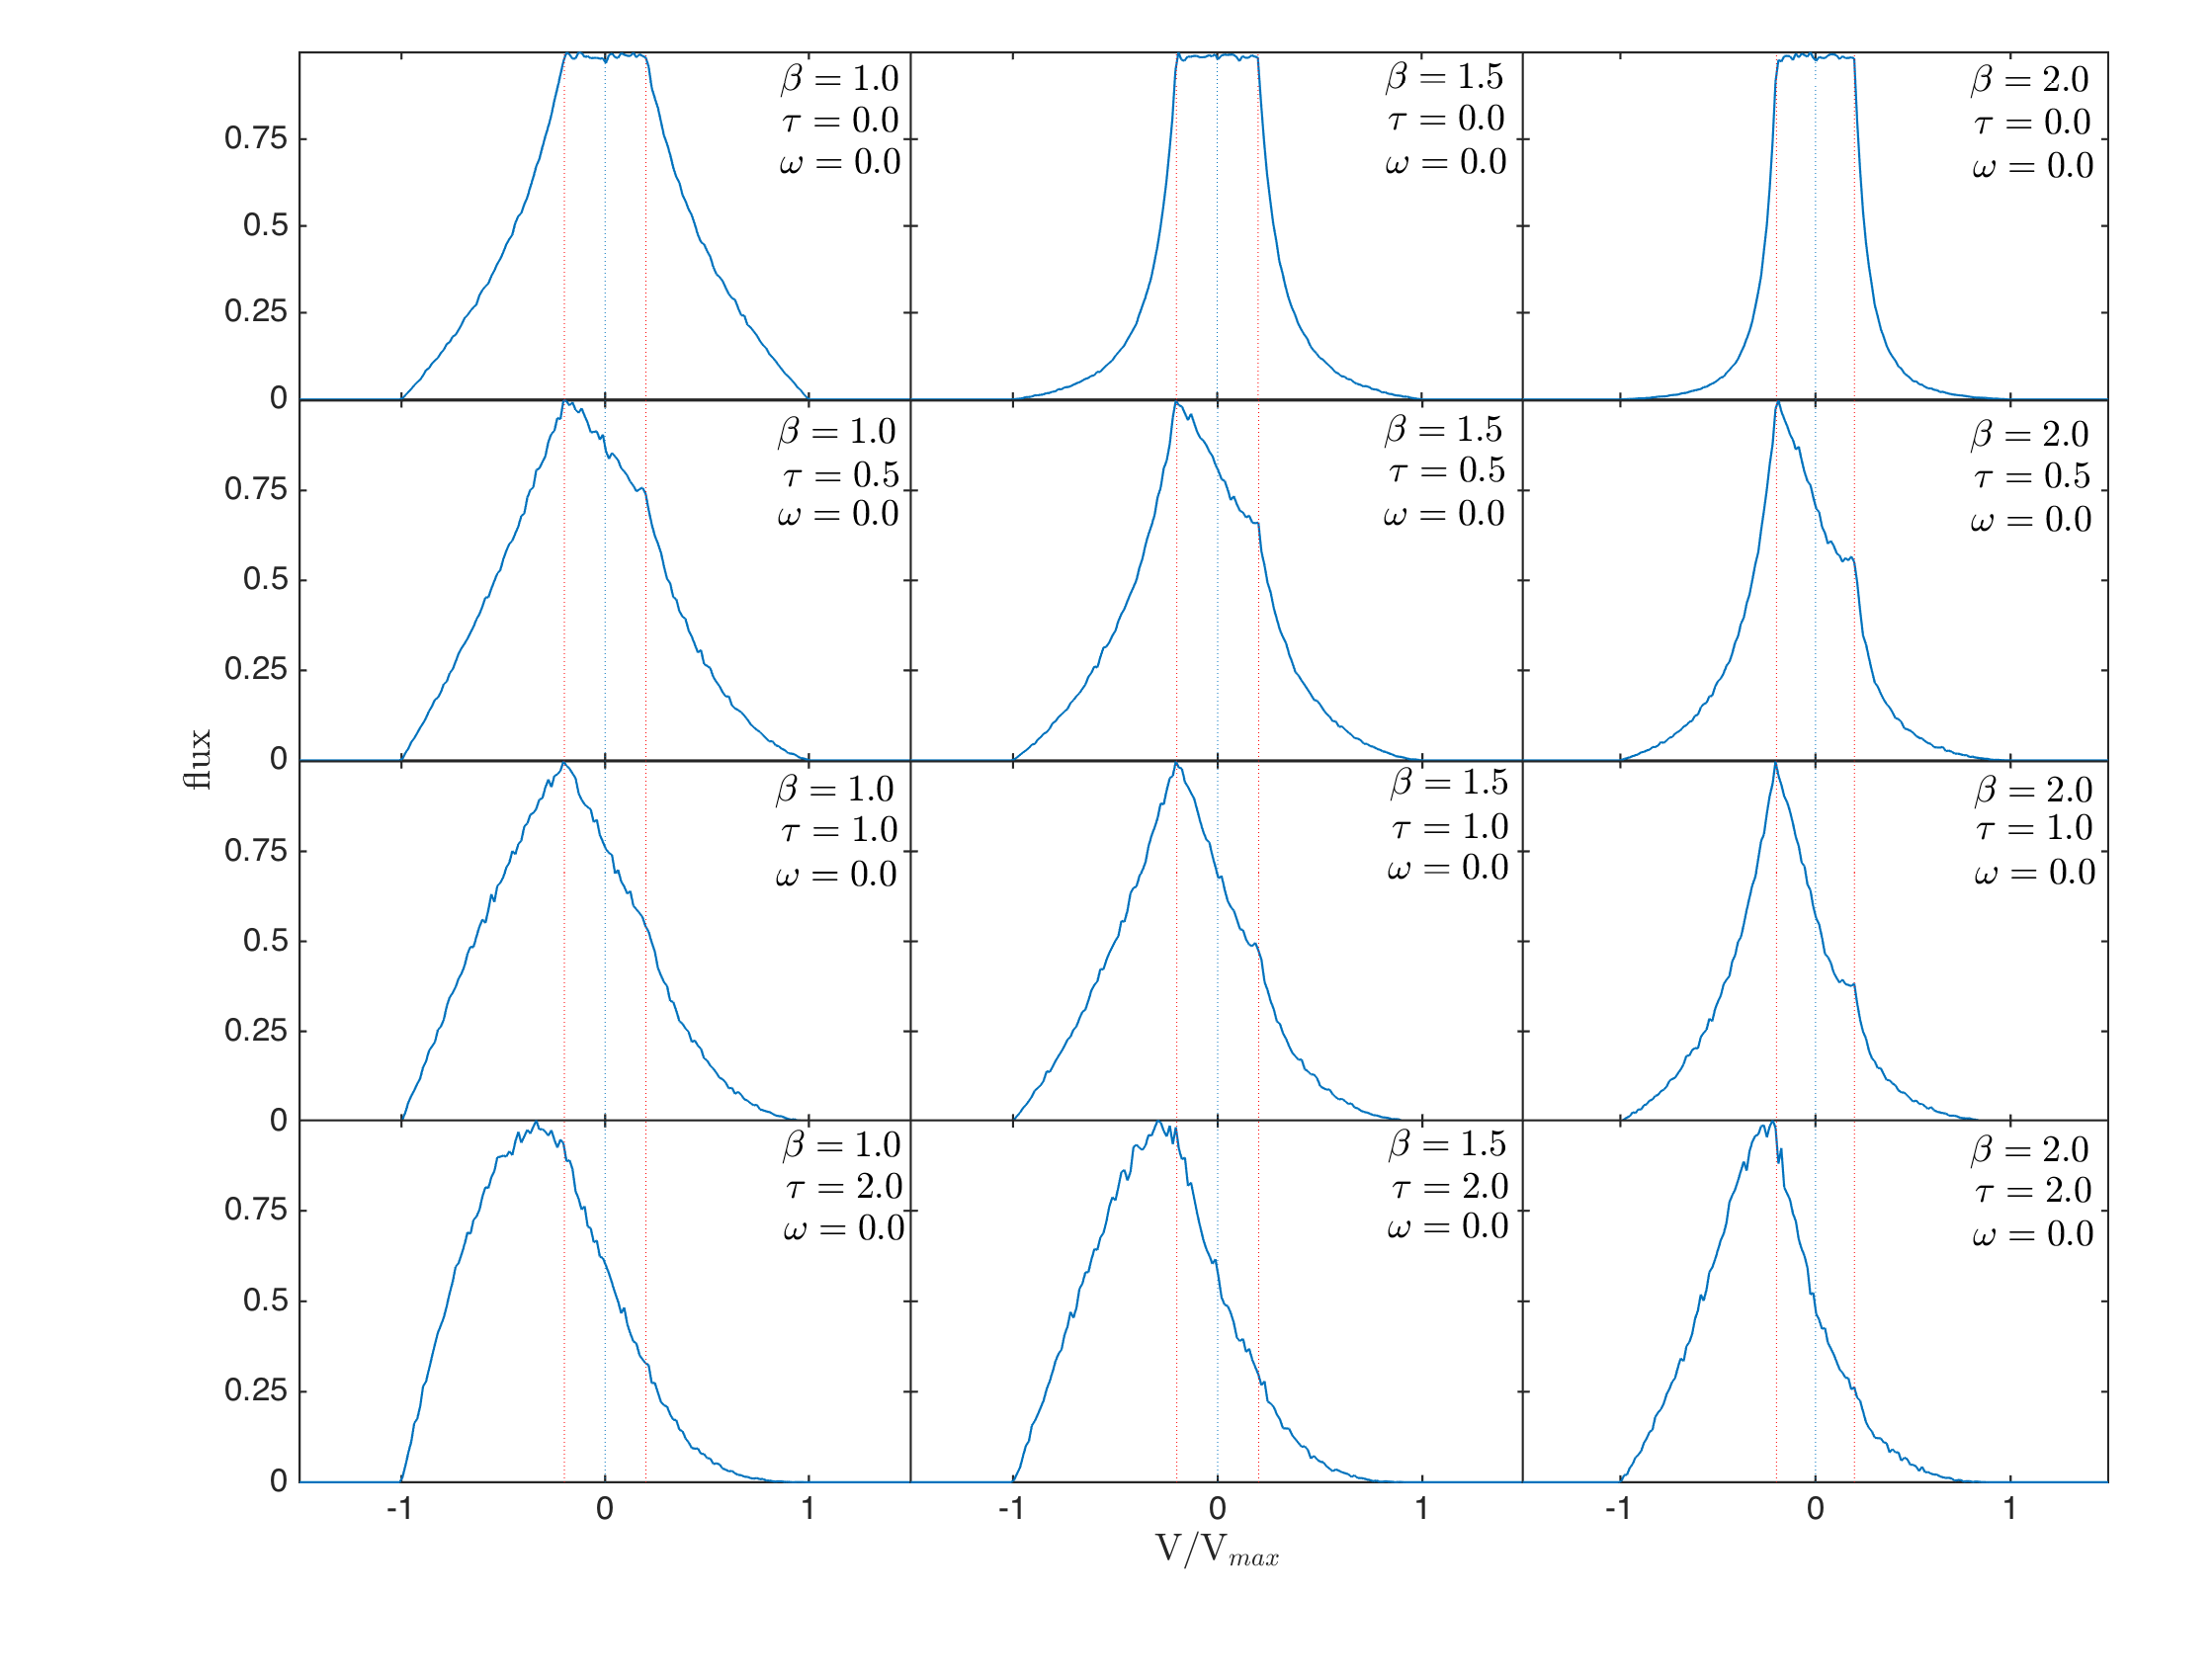
\includegraphics[trim =77 0 6 15,clip=true,scale=0.44]{chapters/chapter4/images/params/D/D_all2}
\caption{Set of models with $i(r) \propto r^{-2\beta}$ for $\beta=1.0$ (left), $\beta=1.5$ (middle) or $\beta=2.0$ (right), $\omega=0$, 
$R_{in}/R_{out}=0.2$, $v(r) \propto r$ and $v_{max}=1$ illustrating the effects of varying 
$\tau$.  Peak fluxes are scaled to unity.}
\label{bt}
\end{figure}


%At high dust optical depths or when the ratio of the inner and outer radii 
%is small, the entire profile is shifted to the blue and the peak moves 
%beyond $-V_{min}$ further into the blue.  The profiles also tend to become 
%more smooth and featureless.  A set of models showing the effects of 
%varying optical depths for different density profiles and dust albedos are 
%presented in Figures \ref{wt} and \ref{bt} with $R_{in}/R_{out} = 0.2$.



\subsubsection{The completely filled nebula case}

To reproduce similar characteristic dust-affected line profiles where the peak of the profile is shifted beyond $-V_{min}$ into the blue is ``easier" for smaller values of $V_{min}$.  The completely filled nebula is therefore effectively analogous to cases of higher optical depths for a detached shell and the same effects that are illustrated in Figures \ref{bt} and \ref{wt} apply.

%NEED MORE HERE - PRESENT A MODEL?

\begin{figure}
\centering
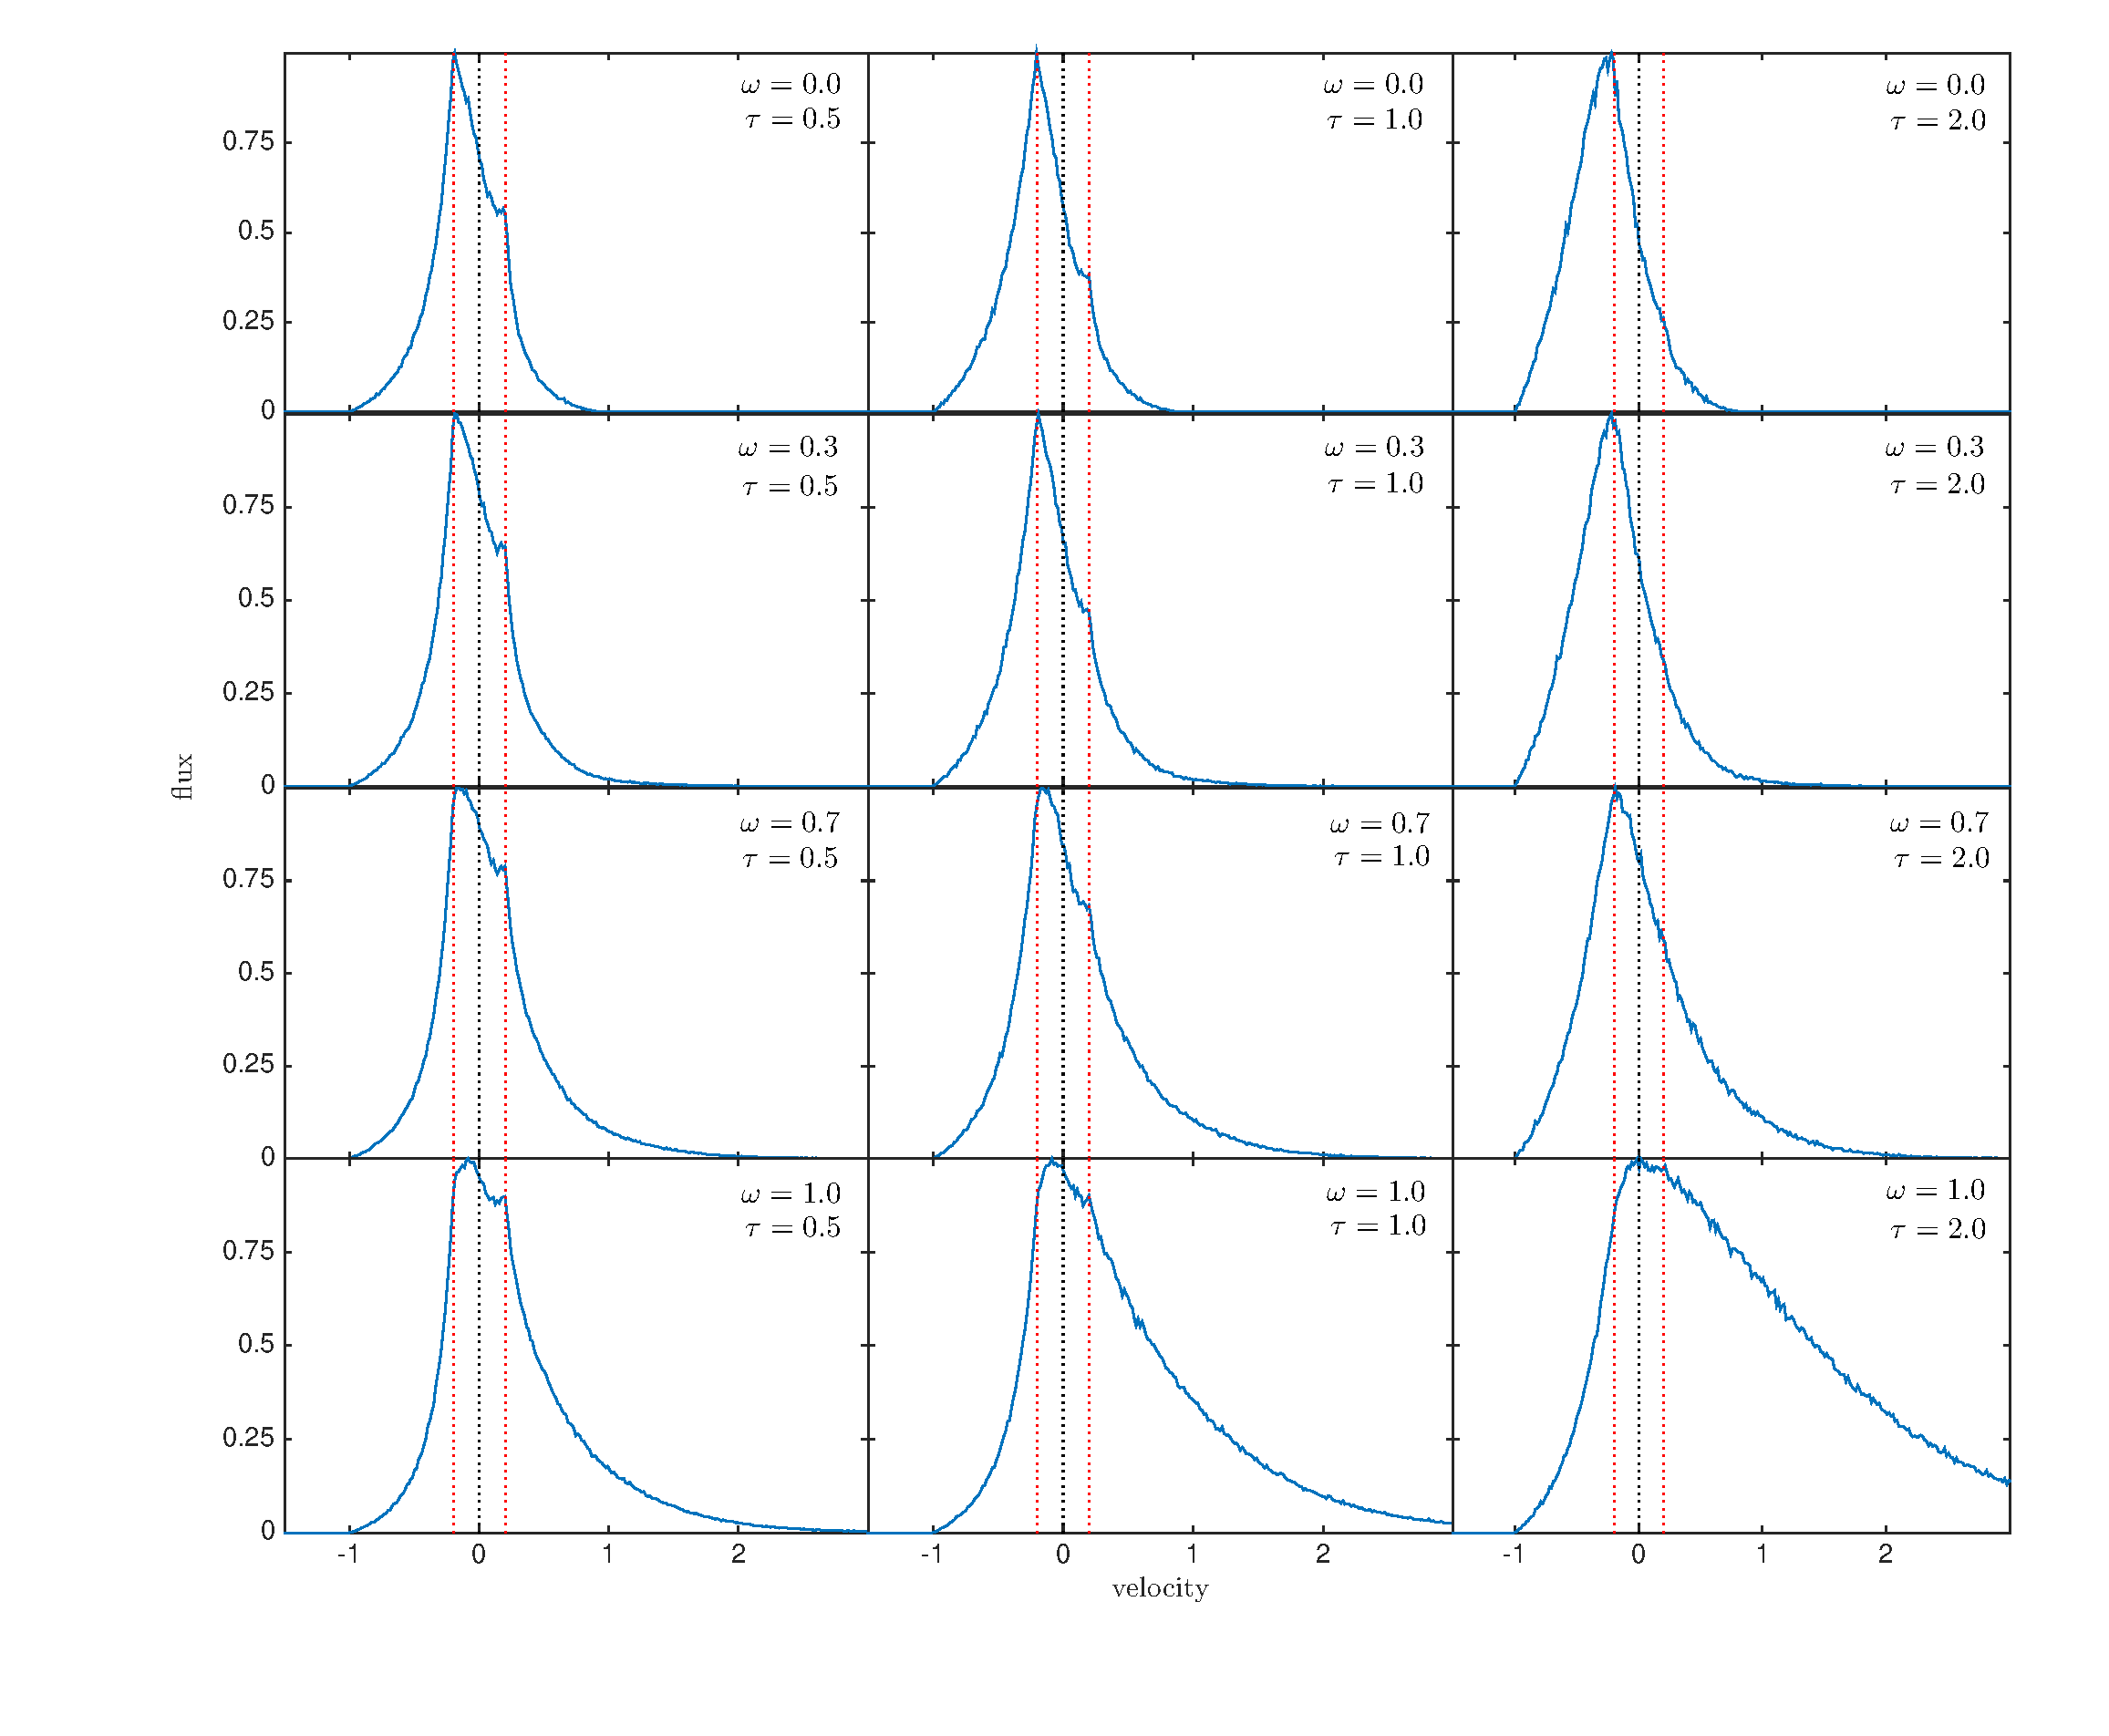
\includegraphics[trim =70 40 40 15,clip=true,scale=0.43]{chapters/chapter4/images/params/C/C_all}
\caption{Set of models with $i(r) \propto r^{-4}$ (i.e. $\beta=2.0$), $R_{in}/R_{out}=0.2$, $v(r) \propto r$  
and $v_{max}=1$ illustrating the effects of varying $\tau$ and $\omega$. 
Peak fluxes are scaled to unity.}
\label{wt}
\end{figure}


\subsection{The dust albedo, $\omega$}
\label{omega}

In the past, there has often been a focus on the effects of absorption by 
dust on the shapes of line profiles and less attention has been paid to 
the potential effects of scattering by dust.  In fact, line profiles can 
be significantly affected by scattering of radiation.  The greater 
attenuation of radiation received from the receding portion of the ejecta 
results in an asymmetry of the line profile whereby the majority of the 
observed emission is located bluewards of the peak.  However, the effects 
of repeated dust scattering events within the ejecta can substantially 
alter the shape of a line profile and potentially can act to counter the 
blue-shifted asymmetry.

Not only does repeated scattering of photons increase the number of 
potential opportunities for a given photon to be absorbed but it also 
results in continuous shifting of the frequency of the photon to the red.  
The photon must do work on the expanding shell of dust in order to escape 
and thus many of the photons are reprocessed beyond the theoretical 
maximum velocity on the red side of the profile.  Even in the case of dust 
grains with a relatively low albedo, a surprisingly persistent wing on the 
red side of the profile is seen, generally beyond the maximum theoretical 
velocity of the emitting region. In the case of strong dust scattering and 
high dust optical depths, this can actively result in a shift in the 
overall asymmetry of the profile, with the majority of the emission being 
emitted redwards of the peak. The peak however, remains blue-shifted (for 
example the bottom left panel of Figure \ref{wt}) or central (for example 
the bottom right panel of Figure \ref{wt}).  For the line profile to 
exhibit this effect requires the dust to be a nearly perfect scatterer;
of the albedos plotted in Figure \ref{albedo_grain}
only the nearly-transparent MgSiO$_3$ sample of \citet{Jager2003}
exhibits such a behaviour.

The combination of relatively low dust optical depths, initially 
flat-topped profiles, greater attenuation on the blue side along with 
increased flux on the red side due to scattering can result in a profile 
that sometimes ends up appearing almost symmetrical, particularly if 
contaminants, such as narrow lines or blending with other broad lines, are 
present or if the resolution of the data is low.  The potential for 
apparently symmetrical profiles that appear to have been uniformly 
blue-shifted should be noted (see Figures \ref{bt} and \ref{wt} for 
examples of this).


\subsection{The dust density profile, $\rho \propto r^{-2\beta}$}
\label{beta}

Whilst the density profile of the dust may have some effect on the 
resulting profiles, it is the initial emissivity profile (dependent on the 
gas density profile) that has the greatest effect on the shape of the line 
profile.  In general, the steeper the emissivity distribution, the 
narrower the line profile becomes.  The sides of the line profile may 
become almost vertical for a very steep distribution since the majority of 
the emission then comes from a very narrow velocity range (see Figure 
\ref{fig:analytics}).  For a flat-topped profile of 
fixed width this approximates the square profile produced in the case of 
an emitting shell with constant velocity.

\begin{figure}

\begin{subfigure}{1\textwidth}
\centering
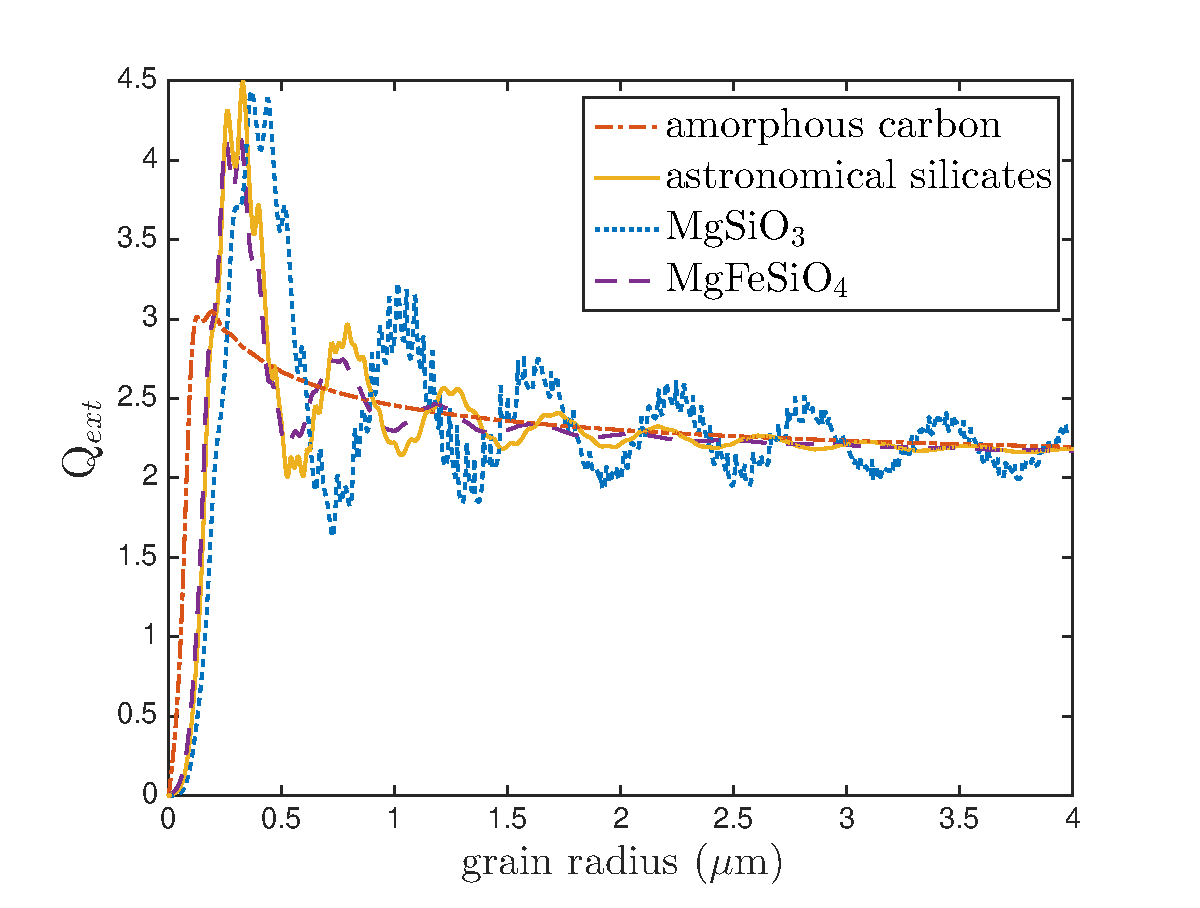
\includegraphics[trim =20 0 45 15,clip=true,scale=0.7]{chapters/chapter4/images/Qext_grainsize_upto4}
\end{subfigure}\\[1ex]
\begin{subfigure}{\textwidth}
\centering
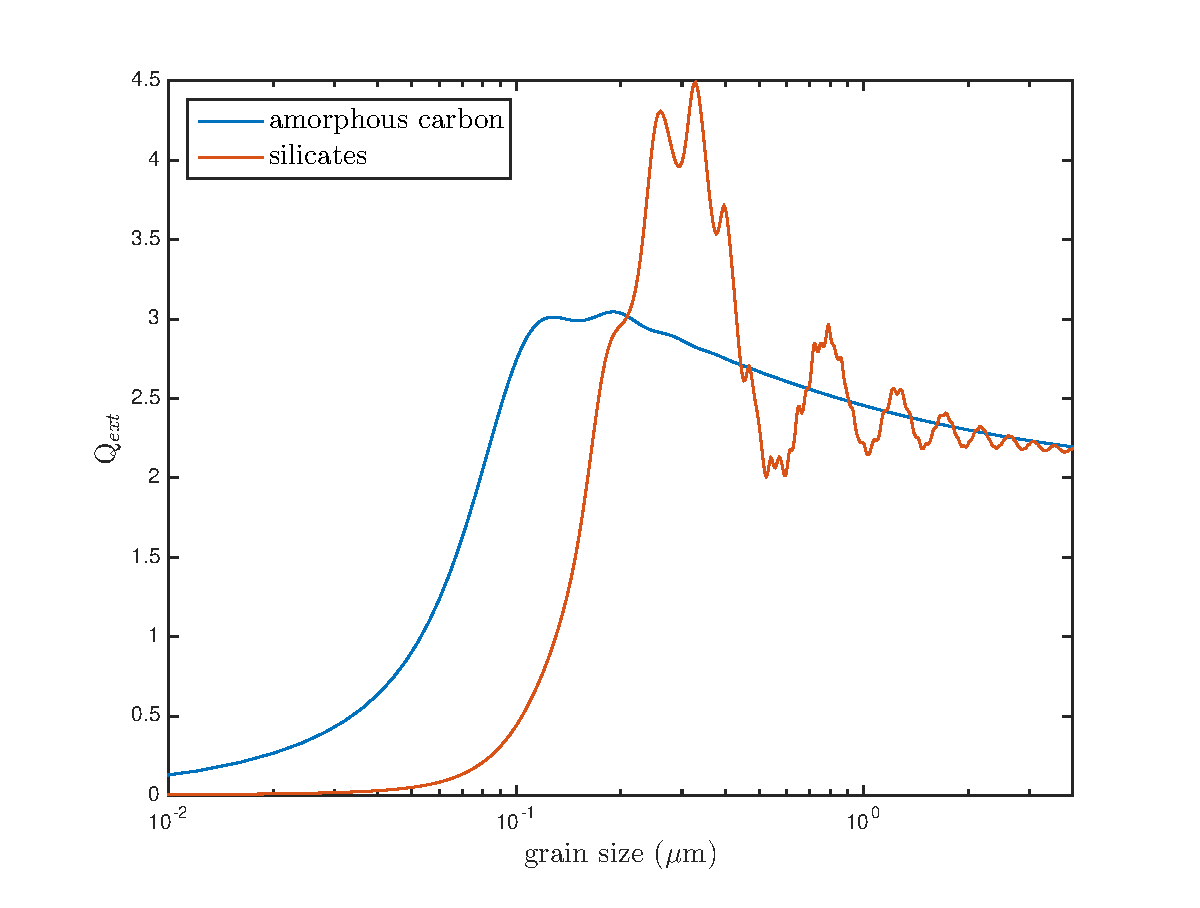
\includegraphics[trim =20 0 45 15,clip=true,scale=0.7]{chapters/chapter4/images/Qext_grainsize_upto4_log}
\end{subfigure}
\caption{The variation of extinction efficiency ($Q_{ext}$) 
with grain radius at $\lambda$ =  656~nm for \citet{Zubko1996} BE amorphous 
carbon, \citet{Draine1984} astronomical silicate and the
MgSiO$_3$ and MgFeSiO$_4$ samples of \citet{Jager2003} and 
\citet{Dorschner1995} respectively. A linear scale is presented on the top and a log scale on the bottom.}
\label{Qext_grain}
\end{figure}

\begin{figure}
\begin{subfigure}{1\textwidth}
\centering
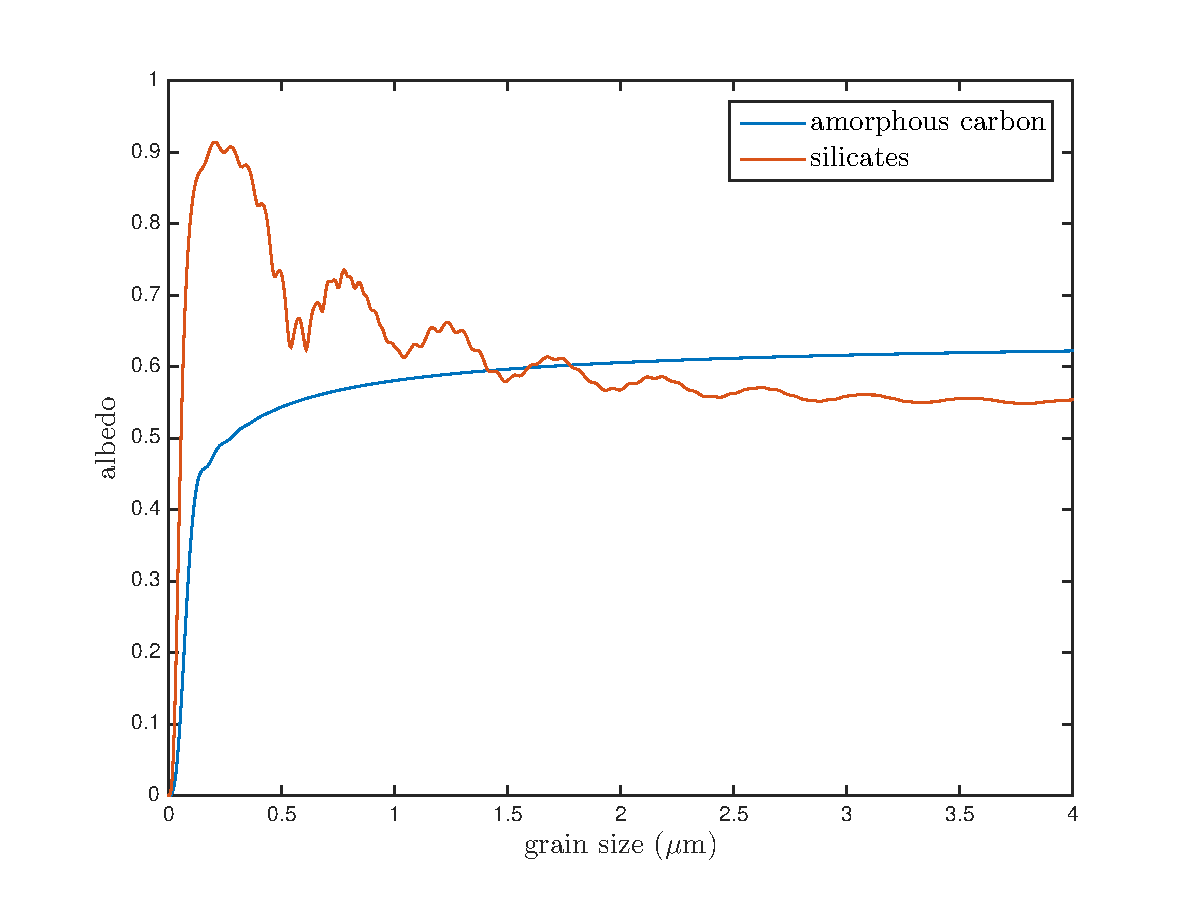
\includegraphics[trim =20 0 45 15,clip=true,scale=0.7]{chapters/chapter4/images/albedo_grainsize_upto4}
\end{subfigure}\\[1ex]
\begin{subfigure}{1\textwidth}
\centering
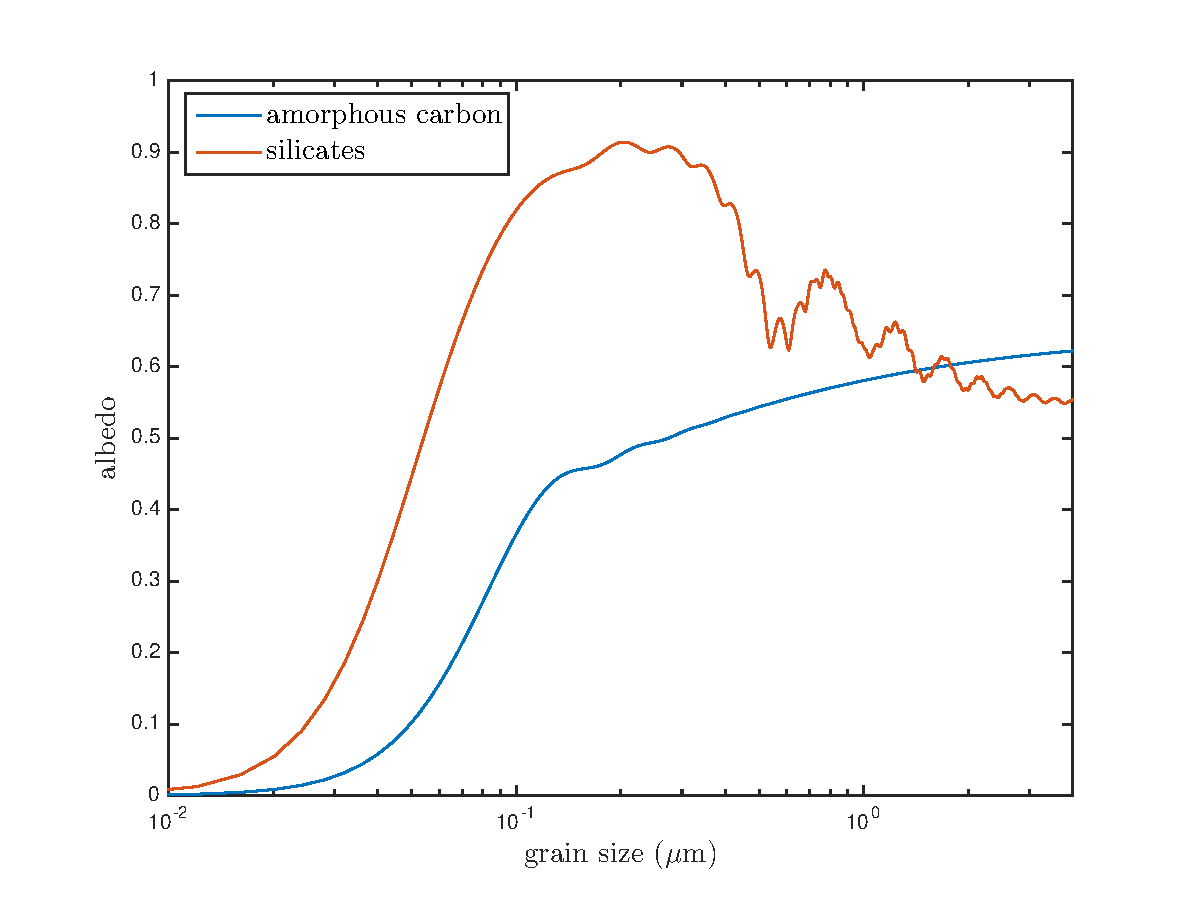
\includegraphics[trim =20 0 45 15,clip=true,scale=0.7]{chapters/chapter4/images/albedo_grainsize_upto4_log}
\end{subfigure}
\caption{The variation of albedo with grain radius at $\lambda$ =  656~nm for \citet{Zubko1996} BE amorphous 
carbon, \citet{Draine1984} astronomical silicate and the
MgSiO$_3$ and MgFeSiO$_4$ samples of \citet{Jager2003} and 
\citet{Dorschner1995} respectively. A linear scale is presented on the top and a log scale on the bottom.}
\label{albedo_grain}
\end{figure}

The dependence of the shape of the line profile on the emissivity 
distribution is described analytically in Section \ref{analytics} for the 
case of very optically thin dust.  However, for even fairly low dust 
optical depths, the density profile plays a significant role in 
determining the shape of the line profile where it is affected by dust 
absorption.  As previously discussed, at relatively small optical depths 
for reasonable $R_{in}/R_{out}$, a section of the flat-topped region is 
removed resulting in a peak at $-V_{min}$.  The shape of the profile in 
this region is significantly affected by the density profile.  Shallow 
density profiles (low $\beta$) produce a virtually linear variation in 
flux between $-V_{min}$ and $+V_{min}$ (for example the profiles in the 
left column of Figure \ref{bt}).  For a fixed dust optical depth, the 
steeper the distribution becomes, the more concave the profile becomes 
between $-V_{min}$ and $+V_{min}$, ultimately resulting in a clear 
shoulder to the profile at $+V_{min}$ (for example the profiles in the 
right column of Figure \ref{bt}).  For extremely steep density 
distributions this can result in a double peaked profile with a trough to 
the red of $V=0$.  An illustration of the effects on the line profiles of 
varying $\beta$ and $\tau$ is shown in Figure \ref{bt}.  As previously 
noted, these features may not be apparent in observed line profiles with 
poor spectral resolution.

\subsection{Inferring properties of the dust from the models}

The presence of an extended red wing at large positive velocities in 
combination with increased extinction on the red side at smaller positive 
velocities can allow the values of $\tau$ and $\omega$ to be well 
constrained.  Where this occurs it is possible to translate these values into a 
dust mass and grain radius for a given species or combination of 
species using grain optical properties and Mie theory (see Figures \ref{Qext_grain} and \ref{albedo_grain}).  


For amorphous carbon, the albedo generally increases with grain radius.  
The presence and extent of any scattering wing on the red side of the 
observed profile can therefore help to place limits on the grain radius.  
However, the greater the grain radius used the smaller the available 
cross-section for interaction per unit dust mass.  Larger masses of dust 
are therefore required to fit the same degree of absorption if a larger 
grain radius is used.  This is in contrast to SED radiative transfer 
modelling where larger grain radii generally result in less dust being 
required to fit the IR portion of the SED (W15).  These two techniques in 
tandem may therefore provide limits on grain radii for different species 
or combinations thereof.

It is known that the use of different optical properties may substantially 
alter dust masses derived using SED fitting for a given species of 
specific grain radius (e.g. \citet{Owen2015}).  However, the use of 
different sets of grain optical constants in our models seems to have only 
a minor effect on the required dust masses, except for cases where the 
albedo is close to unity (pure scattering grains).

\begin{figure}
\begin{subfigure}{0.5\textwidth}
\includegraphics[trim =10 23 25 0,clip=true,scale=0.42]{chapters/chapter4/images/dustdep/a0_001_opt_thin_HaHbPad}
\end{subfigure}
\hspace{4.5mm}
\begin{subfigure}{0.5\textwidth}
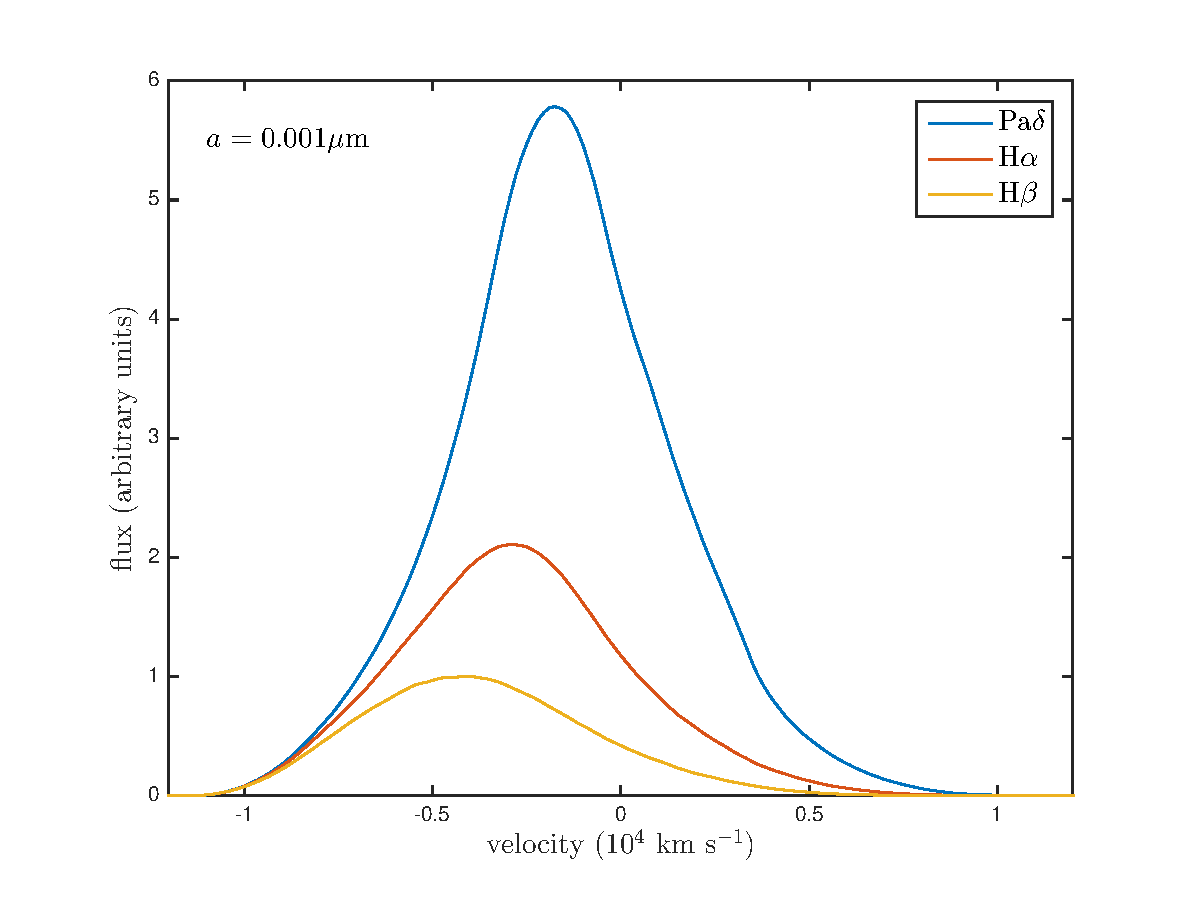
\includegraphics[trim =49 29 25 0,clip=true,scale=0.42]{chapters/chapter4/images/dustdep/a0_001_opt_thick_HaHbPad}
\end{subfigure} \\[1ex]

\begin{subfigure}{0.5\textwidth}

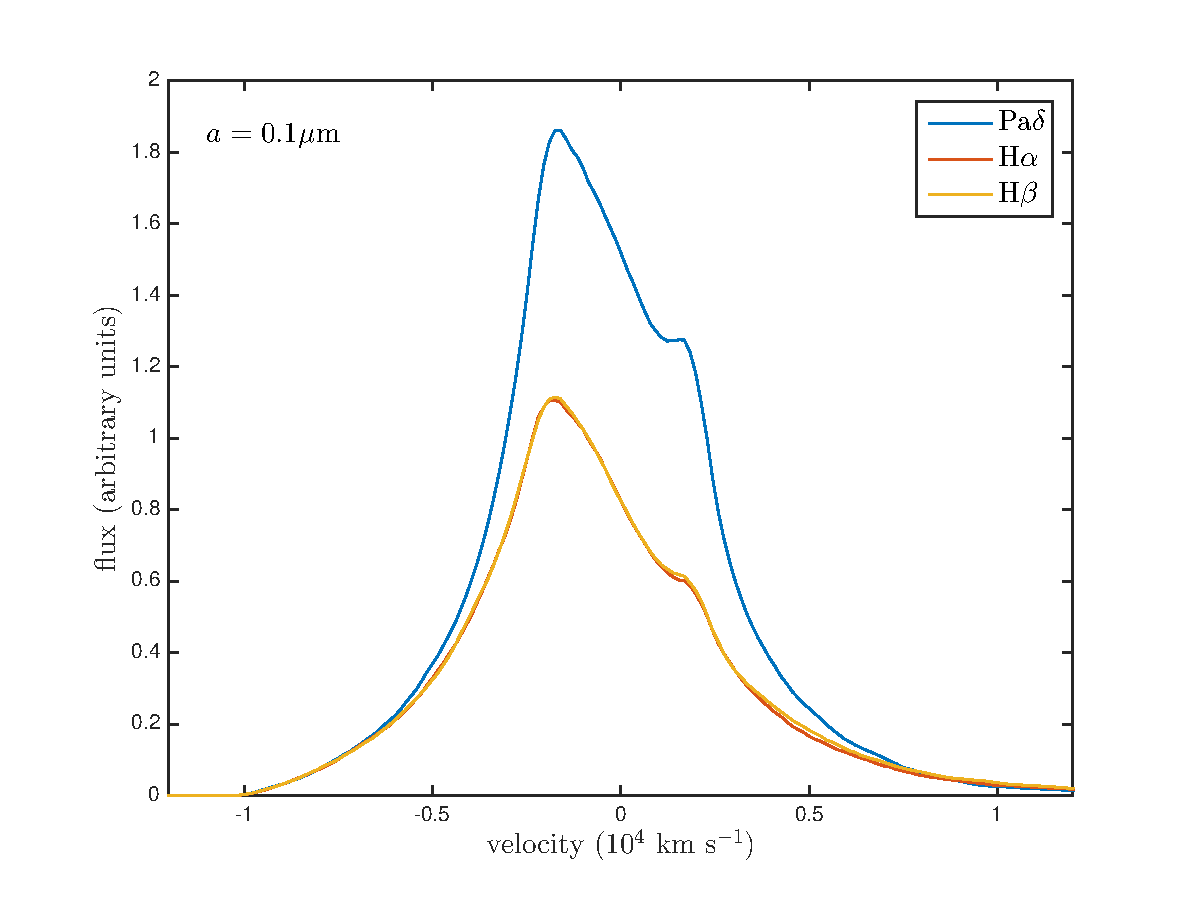
\includegraphics[trim =10 29 25 0,clip=true,scale=0.42]{chapters/chapter4/images/dustdep/a0_1_opt_thin_HaHbPad}
\end{subfigure}
\hspace{3mm}
\begin{subfigure}{0.5\textwidth}
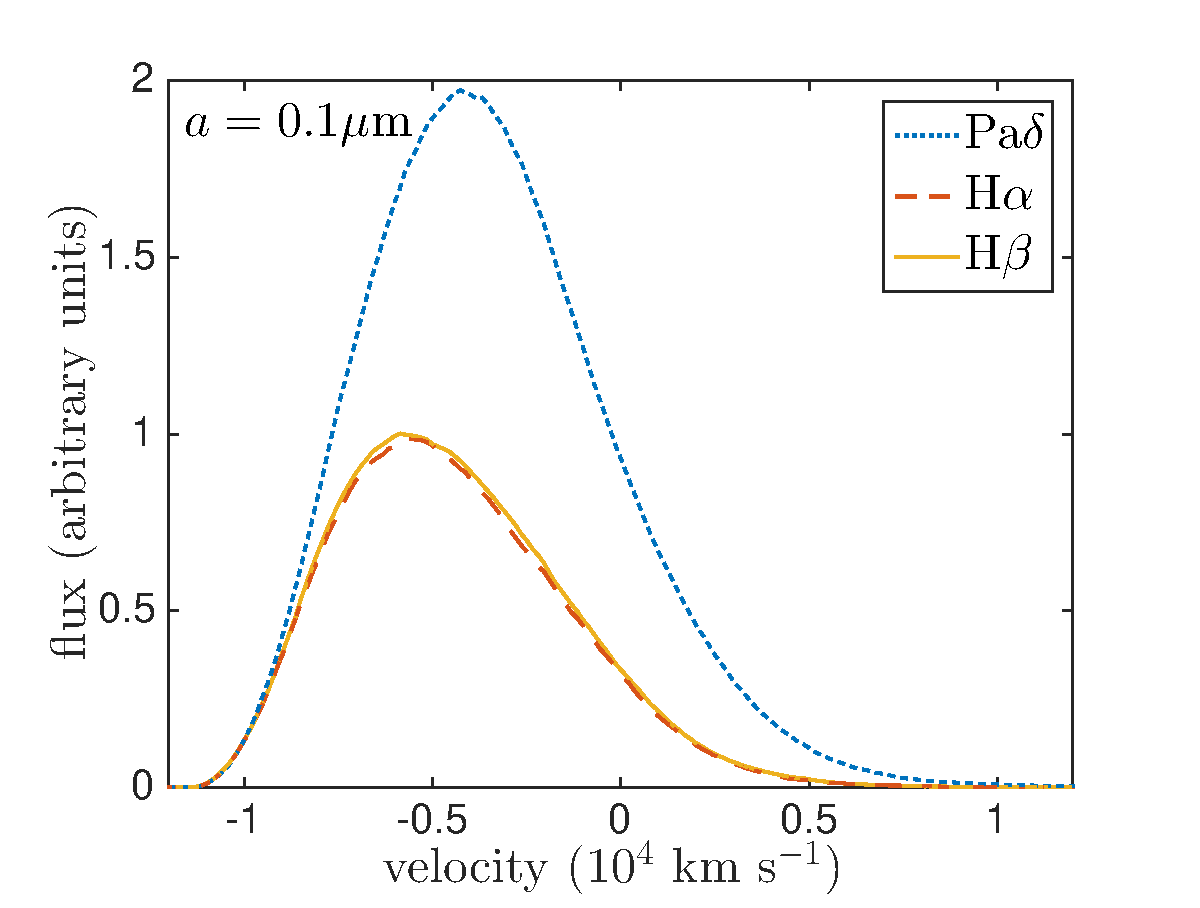
\includegraphics[trim =38 27 45 0,clip=true,scale=0.42]{chapters/chapter4/images/dustdep/a0_1_opt_thick_HaHbPad}
\end{subfigure} \\[2ex]

\begin{subfigure}{0.5\textwidth}
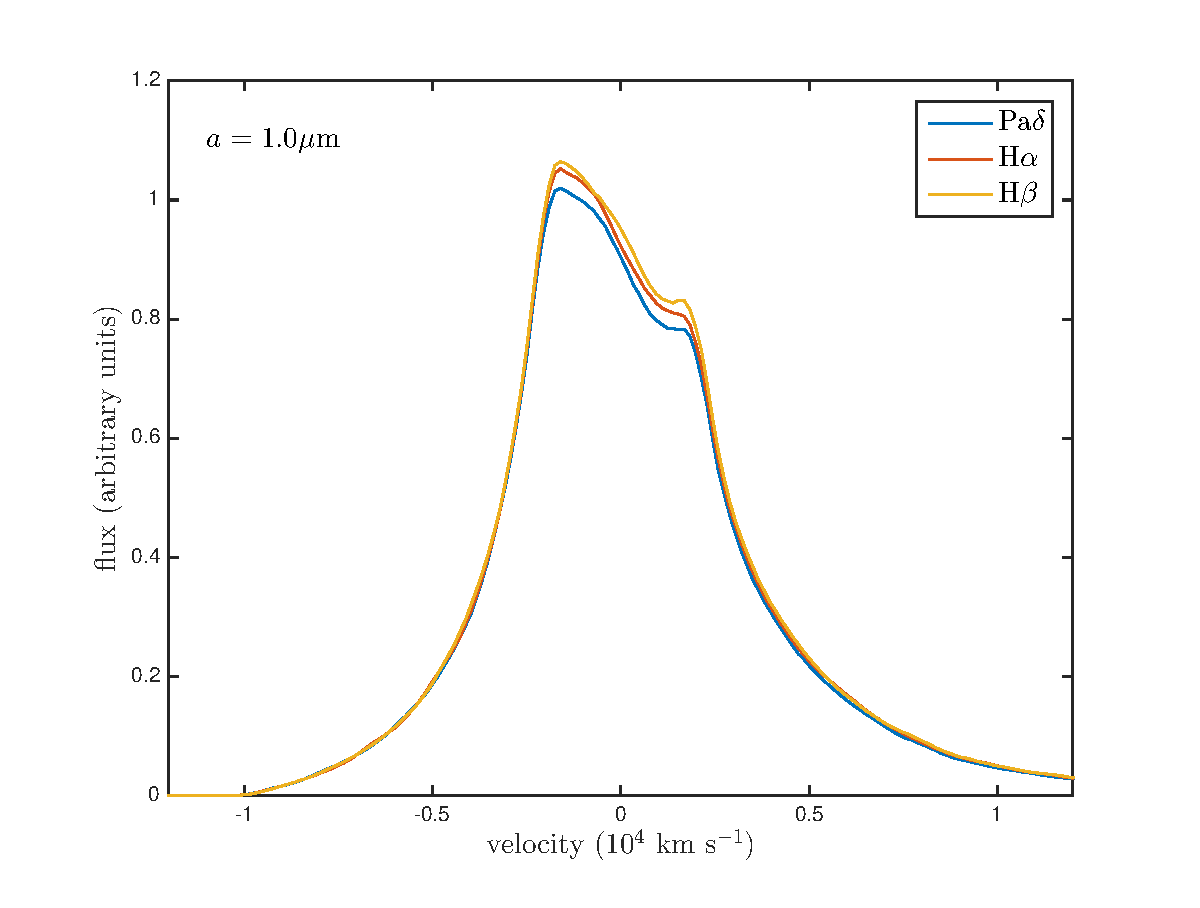
\includegraphics[trim =10 0 25 15,clip=true,scale=0.42]{chapters/chapter4/images/dustdep/a1_opt_thin_HaHbPad}
\end{subfigure}
\hspace{3mm}
\begin{subfigure}{0.5\textwidth}
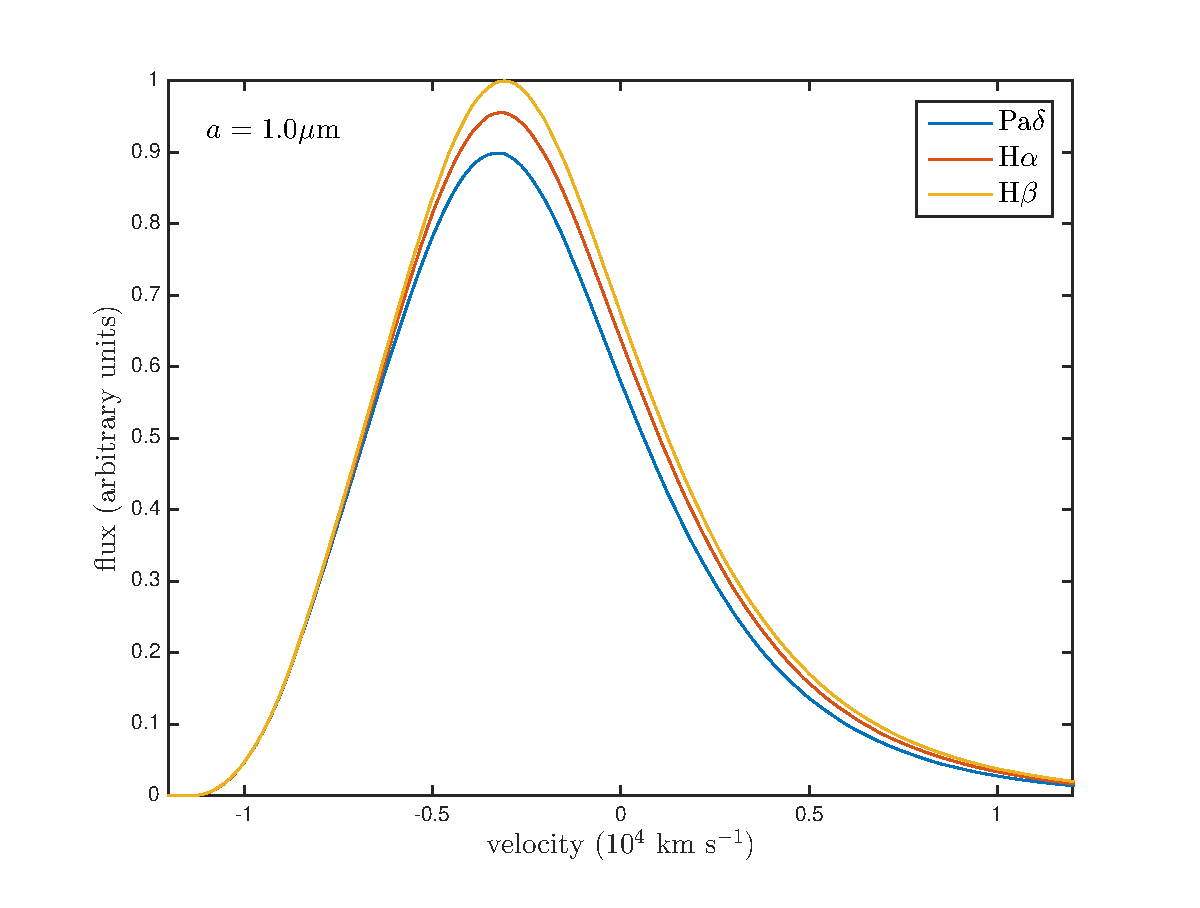
\includegraphics[trim =38 0 45 15,clip=true,scale=0.42]{chapters/chapter4/images/dustdep/a1_opt_thick_HaHbPad}
\end{subfigure}
\caption{Model line profiles for H$\alpha$ (6563\AA\ in red), H$\beta$ (4861\AA\ in yellow) and Pa$\delta$ (10049\AA\ in blue) for optically thin and  optically thick cases on the left-hand side and right-hand side respectively.  All models adopted density profile $\rho(r) \propto r^{-4}$ (i.e. $\beta = 2$), velocity profiles $v(r) \propto r$ and radii ratio $R_{in}/R_{out}=0.2$.  The grain radii used were $a=0.001~\mu$m (top), $a=0.1~\mu$m (middle) and $a=1.0~\mu$m (bottom). All the above models used amorphous carbon.}
\label{wav_dep}
\end{figure}

\begin{figure}
\begin{subfigure}{\textwidth}
\centering
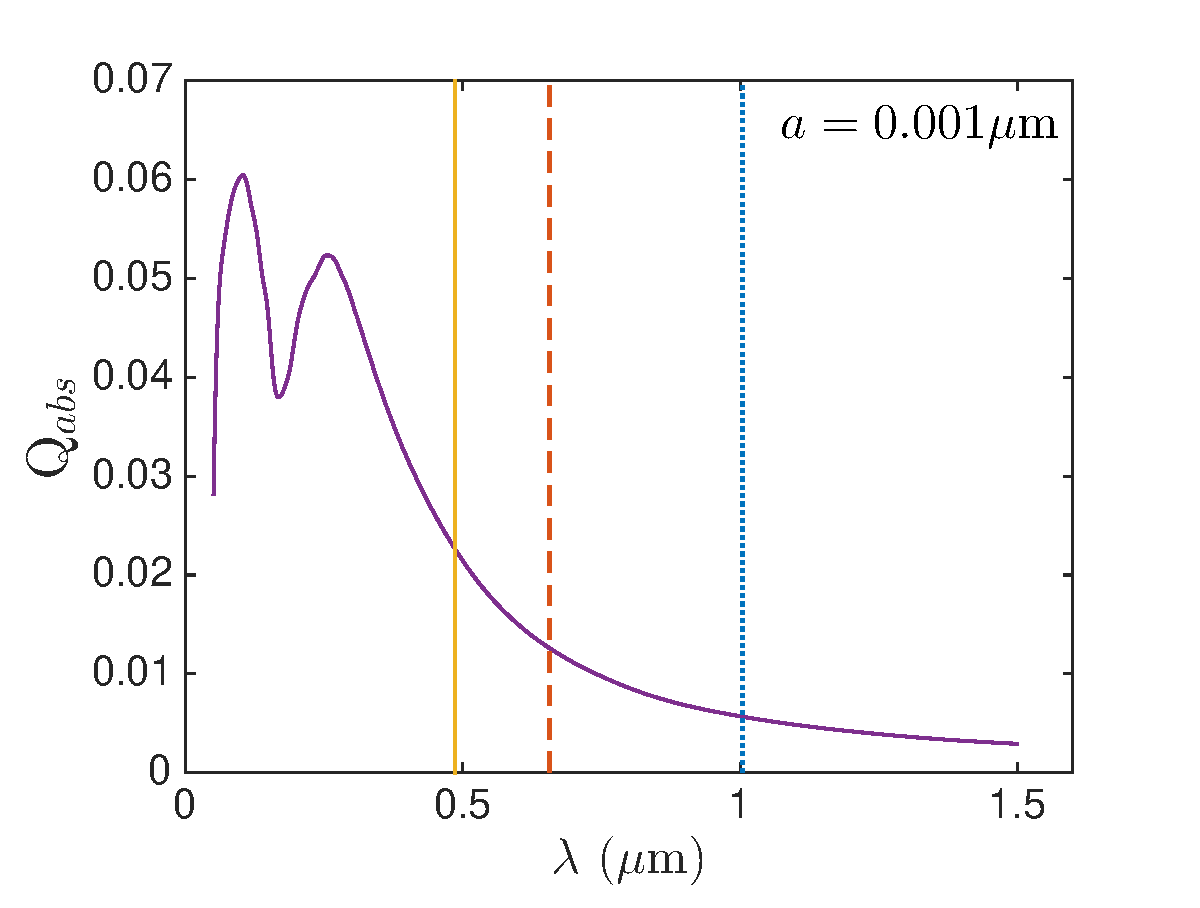
\includegraphics[trim =0 30 45 15,clip=true,scale=0.5]{chapters/chapter4/images/Qabs_a0_001}
\end{subfigure} \\[0.5ex]

\begin{subfigure}{\textwidth}
\centering

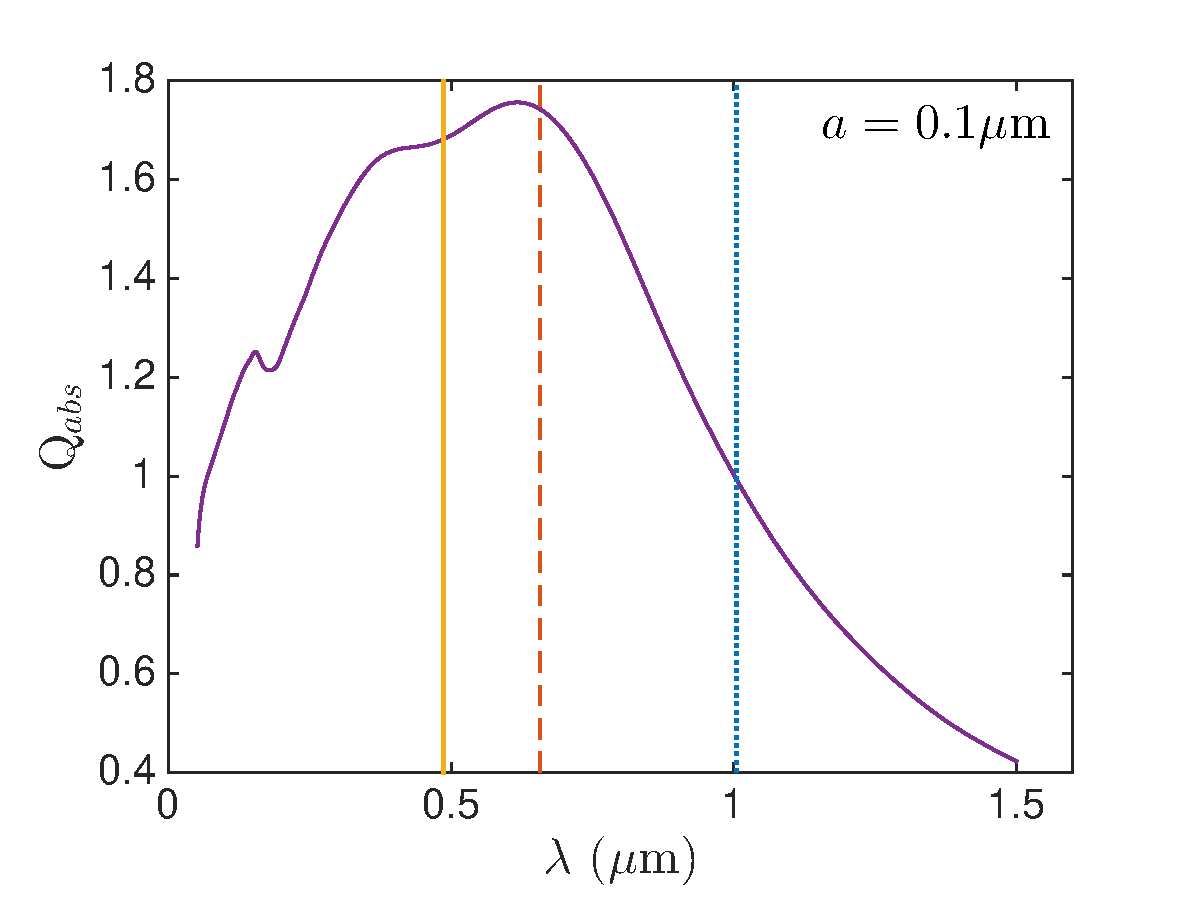
\includegraphics[trim =0 30 45 15,clip=true,scale=0.5]{chapters/chapter4/images/Qabs_a0_1} 
\end{subfigure} \\[0.5ex]

\begin{subfigure}{\textwidth}
\centering
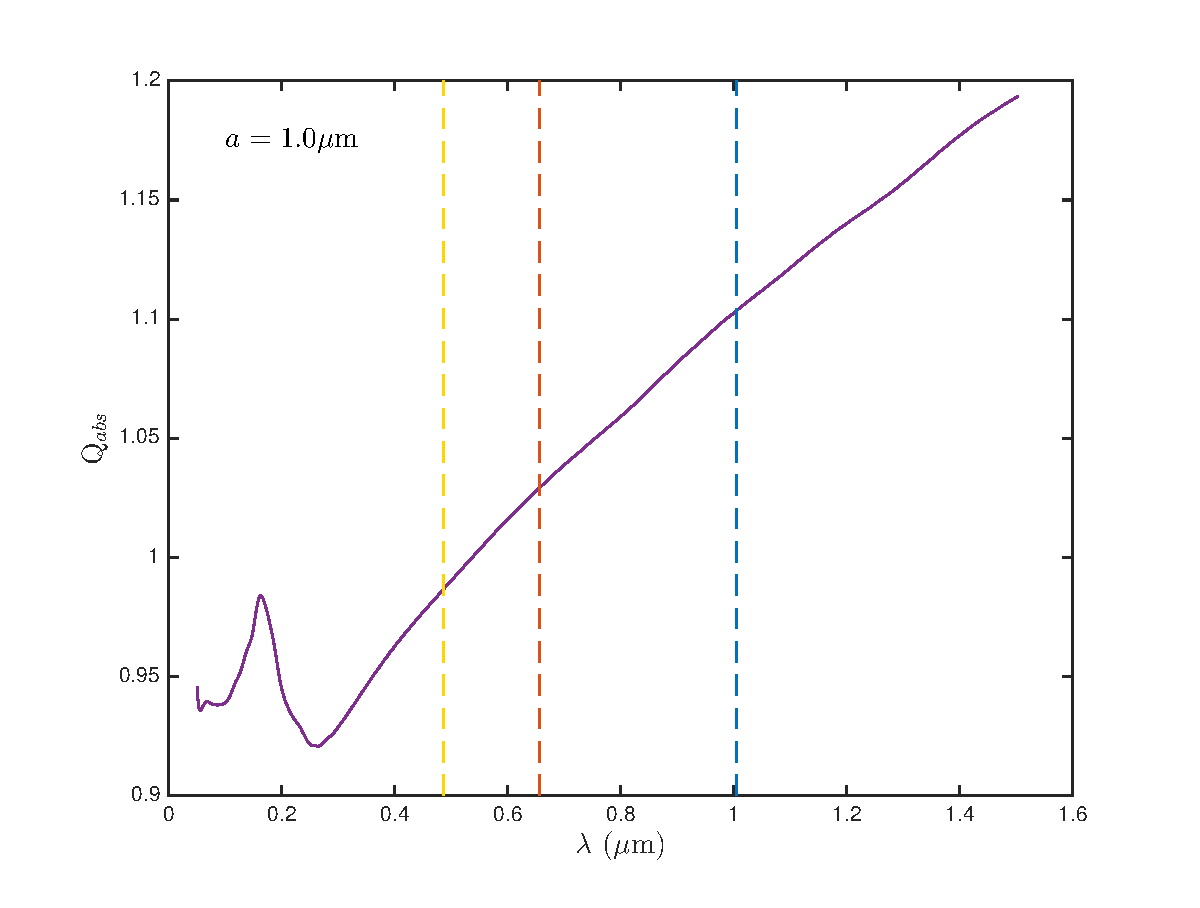
\includegraphics[trim =0 0 45 15,clip=true,scale=0.5]{chapters/chapter4/images/Qabs_a1_0}
\end{subfigure}
\caption{The variation of amorphous carbon dust absorption efficiency with grain radius. The grain radii plotted are $a=0.001~\mu$m (top), $a=0.1~\mu$m (middle) and $a=1.0~\mu$m (bottom).  The vertical lines mark the wavelengths of H$\alpha$ (6563\AA\ in red), H$\beta$ (4861\AA\ in yellow) and Pa$\delta$ (10049\AA\ in blue).}
\label{wav_dep2}
\end{figure}






\subsection{The wavelength dependence of dust absorption}
\label{asym}
The greater the dust optical depth, the more attenuation of the line 
there will be.  As expected, the red side of the profile suffers a greater 
degree of absorption than the blue side.  The resulting asymmetry is 
somewhat more complex than perhaps previously thought.  Dust has 
repeatedly been cited as the agent responsible for the apparent 
blue-shifting of supernova line profiles in the manner of the profiles 
presented in Figure \ref{fig:Lucy}; that is, relatively high optical 
depths result in an overall shift of the entire profile towards the blue.
 The relationship between the blueshifting of the peaks 
of profiles and their wavelength has been discussed by several authors in 
relation to dust formation \citep{Smith2012, Fransson2014, Gall2014}.  
  
In practice a relatively large dust optical depth is required to actively 
shift the peak of the profile bluewards of its natural $-V_{min}$ position 
(corresponding to the velocity at the inner radius of the shell) unless 
this value is very small in comparison to $V_{max}$ i.e. the profile 
originally had a very narrow flat top.  In many cases it seems likely that 
the dust may not be optically thick and the blue-shifting of the peak of 
the profile is just a result of attenuation in the flat-topped section (close 
to $R_{in}$).  The peak would then tend to be located at $-V_{min}$.

Since dust absorption is wavelength dependent for $2\pi a < \lambda$, one 
might expect the position of the peak line flux to be dependent on the 
wavelength of the line being considered.  I note here that whilst 
variations of the peak velocity of a line as a function of line wavelength 
may occur in cases of high dust optical depths or small $R_{in}/R_{out}$, 
this may not be the case for many supernova lines emitted from ejecta with 
low dust optical depths.  The wavelength-dependence of dust absorption 
instead can result in differing degrees of extinction in the flat-topped 
region of each profile but still leave the peak at its blue-shifted 
position of $-V_{min}$.  If this is the case then there would be no reason 
to expect a variation in the position of the peaks of profiles to be 
correlated with the wavelength dependence of dust absorption.  Instead one 
would expect it potentially to trace the location of different ions within 
the ejecta, possibly with different $V_{min}$ values observed for 
different species.

For lines from the same ion, for example the Balmer and Paschen lines of 
HI, we might expect to see peaks at the same position but differing 
degrees of absorption. At high spectral resolutions, it might be possible 
to detect differences in the shapes of the line profiles, particularly 
between $-V_{min}$ and $+V_{min}$ where the steepness of the incline 
traces the degree of dust absorption.  This can be seen in Figure 
\ref{wav_dep} where I illustrate the effects of the wavelength dependence 
of dust absorption for three lines, H$\alpha$ (6563\AA), H$\beta$ 
(4861\AA) and Pa$\delta$ (10049\AA).  All lines were modelled using three 
different grain radii and for both optically thin and thick dust cases.  
I also show in Figure \ref{wav_dep2} the variation of the absorption efficiency with wavelength 
for three different amorphous carbon grain radii.
%The greater the dust optical depth, the more attenuation of the line 
%there will be.  As expected, the red side of the profile suffers a greater 
%degree of absorption than the blue side.  The resulting asymmetry is 
%somewhat more complex than perhaps previously thought.  Dust has 
%repeatedly been cited as the agent responsible for the apparent 
%blue-shifting of supernova line profiles in the manner of the profiles 
%presented in Figure \ref{fig:Lucy}; that is, relatively high optical 
%depths result in an overall shift of the entire profile towards the blue.
% The relationship between the blueshifting of the peaks 
%of profiles and their wavelength has been discussed by several authors in 
%relation to dust formation \citep{Smith2012, Fransson2014, Gall2014}.  
%
%In practice a relatively large dust optical depth is required to actively 
%shift the peak of the profile bluewards of its natural $-V_{min}$ position 
%(corresponding to the velocity at the inner radius of the shell) unless 
%this value is very small in comparison to $V_{max}$ i.e. the profile 
%originally had a very narrow flat top.  In many cases it seems likely that 
%the dust may not be optically thick and the blue-shifting of the peak of 
%the profile is just a result of attenuation in the flat-topped section (close 
%to $R_{in}$).  The peak would then tend to be located at $-V_{min}$.
%
%Since dust absorption is wavelength dependent for $2\pi a < \lambda$, one might expect the 
%position of the peak flux to be dependent on the wavelength of the line being 
%considered.  Whilst this may occur in cases of high dust 
%optical depth, this is not necessarily likely to be seen in the ejecta of 
%most supernovae.  The wavelength-dependence of dust absorption instead 
%can result in differing degrees of extinction in the flat-topped region of 
%each profile but still leave the peak at its blue-shifted position of 
%$-V_{min}$.  Of course, the value of $V_{min}$ may be different for 
%different species.  However, if this is the case then there would be no 
%reason to expect a variation in the position of the peak of profiles to be 
%correlated with the wavelength dependence of dust.  Rather one would 
%expect it potentially to trace the location of different ions within the ejecta. 
%However, for lines from the same ion, for example the Balmer and Paschen lines of HI,
%I might expect to see peaks at the same position but differing degrees of absorption.
%At high resolutions, it might be possible to detect differences in the shape of the line 
%profiles, particularly between $-V_{min}$ and $+V_{min}$ where the steepness of the 
%incline traces the degree of dust absorption.  This can be seen in Figure \ref{wav_dep} 
%where I illustrate the effects of the wavelength dependence of dust absorption for 
%three lines, H$\alpha$ (6563\AA), H$\beta$ (4861\AA) and Pa$\delta$ (10049\AA).  
%All lines were modelled using three different grain radii and in both optically thin and 
%thick cases.  I also show the variation of the absorption cross-section with 
%wavelength at three different grain radii in Figure \ref{wav_dep2}.
%
%The attenuation of the flat-topped region is  often such that it can 
%be hard to discern a difference in slope between the attenuated 
%section between $-V_{min}$ and $+V_{min}$ and the slope of the wing for 
%$V>+V_{min}$, particularly in circumstances where data is of poor 
%resolution or has a poor signal-to-noise ratio.  Even in the case of 
%excellent data, it may be easy to overlook these particular features or to 
%dismiss them as natural fluctuations in the geometry of the ejecta rather than 
%that they may be a product of dust absorption effects.
%
%The greater attenuation of radiation received from the receding portion of 
%the ejecta results in an asymmetry of the line profile whereby the 
%majority of the observed emission is located bluewards of the peak.  
%However, the effects of repeated dust scattering events within the 
%ejecta can serve to counter this asymmetry.  Even in the case of dust grains 
%with a relatively low albedo, a surprisingly persistent wing on the red 
%side of the profile is seen beyond the maximum theoretical velocity 
%of the emitting region.  For higher albedos this can actively result in a 
%shift in the overall asymmetry of the profile, with the majority of the 
%emission being emitted redwards of the peak, though the peak itself 
%remains blue-shifted.
%
%This effect is obviously analogous to that of electron scattering which 
%also produces a significant red wing in line profiles \citep{Hillier1991, 
%Auer1972}. This is an important consideration in both modelling and 
%analysis of spectral line profiles.  DAMOCLES has the capacity to include 
%a basic electron scattering mechanism in order to assess the possibility 
%that any observed red wing might be produced by electron scattering rather 
%than dust scattering.  The red wing observed in line profiles is an 
%excellent diagnostic for determining the overall dust albedo and it is 
%therefore important to establish whether this feature is due to 
%electron or dust scattering or a combination of the two.
%
%The combination of relatively low optical depths, initially flat-topped 
%profiles, greater attenuation on the blue side with increased flux on the 
%red side due to scattering can result in a profile that ends up appearing 
%almost symmetrical, particularly if 
%contaminants, such as narrow lines or blending with other broad lines, are 
%present or if the resolution of the data is low.  The potential for apparently 
%symmetrical profiles that appear to have been uniformly blue-shifted 
%should be noted (see Figures \ref{bt} and \ref{wt} for examples of this).



\subsection{The effect of a grain radius distribution}
\label{gs_distn}
It is important to consider the potential effect on the dust mass of modelling a grain radius distribution instead of a single grain radius.  For a grain radius distribution the overall extinction cross section, $C_{ext}$, at a given wavelength is calculated as
\begin{equation}
C_{ext}=\int^{a_{max}}_{a_{min}} Q_{ext}(a) n(a) \pi a^2 da 
\end{equation}

where $Q_{ext}(a)$ is the extinction efficiency for a grain radius $a$ and $n(a)$ is the number of grains with size $a$. The overall extinction efficiency is then
\begin{equation} 
Q_{ext} = \frac{C_{ext}}{ \int^{a_{max}}_{a_{min}} n(a) \pi a^2 da} 
\end{equation}
 
The scattering cross-section $Q_{sca}$ is similarly calculated.  As a result of these calculations, there is rarely a single grain radius that has the same albedo and extinction efficiency as a size distribution.  Modelling a size distribution instead of a single grain radius may therefore alter the deduced dust mass.  Since models are only sensitive to the optical depth and the albedo, however, it is not possible to deduce the grain radius range or distribution and only single grain radii are investigated in the models that are presented in the following chapters.

Whilst this apparently limits the scope of these results, it is important to consider the extent to which considering grain radius distributions would alter the derived dust masses.  For each model that I construct, I derive a dust mass for a given species at a single grain radius.  By considering the equation that determines the optical depth for both a single grain radius and a grain radius distribution, I can 
%By considering a number of grain radius ranges and adopting a power law distribution with a variable exponent, I may gain some insight into the effects of adopting a distribution rather than a single size.  For the classical MRN power law ($n(a) \propto a^{-3.5}$) with a wide grain radius range ($a_{min} = 0.001 \mu$m to $a_{max} = 4.0 \mu$m) the derived albedo of $\omega=0.001$ is much too small to reproduce the required wing seen at early epochs.  I investigate this issue by adjusting the exponent of a distribution for a number of grain radius ranges until the overall albedo is the same as that seen for the best fitting single grain radius.  
approximately calculate the required dust mass for a distribution of grain radii from the properties of a single-size model by equating the optical depths.  The optical depth for a single grain radius is proportional to 
\begin{equation}
\tau_{\nu} \propto Q_{ext,\nu}(a)  \sigma(a) n_d
\end{equation}

\noindent where $n_d$ is the number density of dust grains, $\sigma(a)$ is the cross-sectional area of a grain of radius $a$ and $Q_{ext,\nu}(a)$ is the extinction efficiency for a grain of radius $a$ at frequency $\nu$.  On average, this gives
\begin{equation}
\tau_\nu \propto \frac{Q_{ext,\nu}(a) M \pi a^2}{\frac{4}{3} \pi a^3 \rho V} \propto \frac{Q_{ext,\nu}(a) M}{\frac{4}{3} a \rho V}
\end{equation}

\noindent for a total dust mass $M$, total volume of the ejecta $V$ and density of a dust grain $\rho$.

By equating the equations for the total dust optical depth for a single grain radius and a distribution of grain radii, we obtain (at a specific frequency)
\begin{equation}
\label{distn_conv}
M_{d}= \frac{M_s Q_{ext,s}(a_s)}{a_s} \times \frac{\int^{a_{max}}_{a_{min}} n(a) a^3 da}{\int^{a_{max}}_{a_{min}} Q_{ext}(a) n(a) a^2 da}
\end{equation}

where the subscript $s$ represents the single grain radius quantities and the subscript  $d$ represents quantities for the grain radius distribution.  This is only calculable for a specific wavelength and is therefore only an approximate conversion when performed at the rest-frame wavelength of the line in question.  However, practically, the variation of extinction efficiency and albedo over the narrow wavelength ranges modelled within the code is not significant and so this method produces relatively accurate dust masses (corroborated by running models with the new parameters).

\subsection{The effect of different species}
%CHECK THIS SENTENCE WHEN ALL MODELLING DONE
In the majority of the modelling that follows, a single species, amorphous carbon, is considered.   A single species is used since the parameters that affect the quantity of dust required in the model are the albedo and the optical depth.  There are therefore  likely many possible combinations of species that may result in a good fit to the data.  The choice of amorphous carbon is partly motivated by evidence that, for SN~1987A (which, as an very well-observed, local core-collapse supernova, is an excellent test case) the fraction of silicates present in the dusty ejecta is limited to approximately 15\% \citep{Ercolano2007,Wesson2015}.  It is also motivated by previously published SED models which generally employ amorphous carbon.  This is because SED models frequently require far larger masses of silicate dust than more absorbing amorphous carbon dust in order to produce similar levels of infrared flux and therefore amorphous carbon models are likely to produce the more conservative dust mass estimates.  By modelling with amorphous carbon I may compare directly to these SED models where possible.

I consider the change in dust mass when an alternative dust medium is used instead of amorphous carbon.  I use a generic silicate dust medium as an illustrative example.
%I use the optical constants presented in \cite{Draine1984}. 
 In a similar manner to the approach detailed in Section \ref{gs_distn}, I may calculate the mass of silicates that is equivalent to an amorphous carbon mass for a single grain radius.  I consider the albedo at the original grain radius, calculate the equivalent grain radius for silicates that results in the same albedo and then calculate the new dust mass by considering the change in the extinction efficiency as
\begin{equation}
\label{species_conversion}
M_{sil} = M_{amc} \Big( \frac{Q_{amc}}{Q_{sil}} \Big) \Big(\frac{a_{sil}}{a_{amc}}\Big) \Big(\frac{\rho_{sil}}{\rho_{amC}}\Big)
\end{equation}

%Due to the nature of the variation of albedo with grain radius for silicates (see Figure \ref{albedo_grain}), there is often more than one silicate grain radius that will give rise to the same albedo.  

I will make use of the above ``conversion" equations in the next chapter when I consider various models of SN 1987A and discuss the effects of varying both species and grain radius.

%I consider all the possibilities and the resulting mass conversion factors in Table \ref{tb_sil}.  In my best fitting models for days 714 and 806, using any fraction of silicates of either grain radius would serve to increase the dust mass.  However, at later epochs, using some fraction of silicate dust would reduce the dust mass to potentially more than half of my estimated values. However, this is still within my predicted range and my minimum and maximum dust masses remain robust.
%
%\begin{table}
%	%\begin{minipage}{180mm}
%	\caption{Equivalent dust masses for the day 714 clumped models using grain radius distributions and 100\% amorphous carbon. $f$ is factor of increase from the dust mass for the single size model ($M=7 \times 10^{-5} M_{\odot}$ with $a=0.6 \mu$m) and $p$ is the exponent of the grain radius distribution $n(a) \propto a^{-p}$.}
%	\label{tb_sil}
%	\begin{center}
%  	\begin{tabular}{@{} cccccc @{}}
%    	\hline
%	\multicolumn{2}{c}{\textit{carbon}} && \multicolumn{2}{c}{\textit{silicates}} & \\
%$a$ & $Q_{ext}$ & &$a$& $Q_{ext}$ & $f=M_{sil}/M_{amc}$ \\
%\hline
%0.6 & 2.60633 & &0.0583 & 0.0772 & 5.37 \\
%0.6 & 2.60633 & &4 & 2.1828 & 13 \\
% \\
%3.5 & 2.2129 & &0.0641 & 0.10182 & 0.65 \\
%3.5 & 2.2129 & &1.02 & 2.149 & 0.49 \\
%3.5 & 2.2129 & &1.376 & 2.3514 & 0.61 \\
%
%
%    \hline
%  \end{tabular}
%  \end{center}
%%\end{minipage}
%\end{table}

\subsection{The velocity distribution}

\label{scn:vel_prof}

I do not thoroughly investigate the effects of varying the steepness of the velocity distribution since the influence of this parameter is thoroughly detailed from a mathematical perspective in Section \ref{analytics}.  Simply, the steeper the velocity distribution, the steeper the slope of the sides of the output line profile.  In this sense, there is some degeneracy with the exponent of the density profile.  The steepness of the velocity distribution also affects the width of the flat-topped region of the profile via Equation \ref{eqn:flattop}.  One of the primary reasons that this variable is not investigated in more depth is that all models of late-time line profiles from the ejecta of supernovae adopt a free expansion velocity law $v \propto r$ until the remnant reaches a much later stage of its evolution.  However, by this point the remnant will likely no longer be visible in the optical or IR.

\section{Conclusions}

Throughout this chapter, I have discussed the various ways in which I tested DAMOCLES against both theoretical line profiles derived from first principles and previously published models, and have presented example profiles illustrating the excellent agreement between them.  For each parameter of interest, I have described the manner in which its variation affects different aspects of the emergent line profile.  I have also discussed the effects of altering the properties of the dust itself and have calculated the degeneracies relating to grain radius distributions and composition.  This allows for any model with a given set of dust properties to be easily compared to a model with the same intrinsic geometry but with a different dusty medium.  

This investigation of parameter space resulted in some very interesting insights that may prove important when considering dust formation in the ejecta of CCSNe in the future.  Historically,  a line profile that was flux-biased towards the blue with a blue-shifted peak was considered to be potentially indicative of dust formation.  Whilst this is undeniably the case, it seems likely that a number of other features may also point towards the formation of dust in the ejecta.  I have discussed the presence of an extended red-scattering wing and the lack of a need for asymmetry.  I have also mentioned the possibility of symptomatically jagged profiles, often with sharp inflection points around the value of the minimum velocity ($\pm V_{min}$).  The presence of any or all of these features in the line profiles of the spectra of CCSNe may suggest the presence of newly-formed dust.  In addition to these results, the process of exploring parameter space greatly aided me in modelling SN 1987A and the several other supernova remnants taht are presented in the following chapters.






\clearthesisemptydoublepage
\chapter{The Evolution of Dust Formation in SN~1987A}\label{chp:chp5}

\begin{flushright}
  {\em QUOTE GOES HERE }\\

\ \

\normalsize
{AUTHOR}  
\end{flushright}

\section{10,000 days of SN 1987A}

On 23 February 1987, a star died in an explosion that would inform our understanding of core-collapse supernovae for decades to come.  SN 1987A is uniquely important to the study of supernovae.  At only 50kpc away in the Large Magellanic Cloud (LMC) and as the brightest supernova to be observed since SN1604 (Kepler), it has provided an unprecedented opportunity for studying every aspect of supernovae imaginable.  Since its explosion, SN 1987A has been continuously observed across the entire wavelength range providing a wealth of data to be interpreted.

SN 1987A was the first supernova to be detected via the emission of neutrinos.  Hours before the visible light from SN1987A reached Earth, 19 neutrinos were simultaneously detected in various locations across the globe confirming the core-collapse theory of supernovae \citep{Bionta1987,Hirata1987}.  However, the expected neutron star resulting from this collapse still has yet to be detected.  Various theories exist for this non-detection such as the possibility that a black hole formed instead or that dust is obscuring the light from the star.

Four days after its initial detection, the progenitor star was identified as a blue supergiant \citep{Sonneborn1987}.  Mass ejection from this progenitor star resulted in the complex system of circumstellar rings that are observed around SN 1987A (see Figure \ref{}).

\section{Spectral Observations of SN 1987A}
\label{spectra}
%This is just the archival spectra section of the paper

%%%%%%%%%%%%%%%%%%%%   SPECTRA   %%%%%%%%%%%%%%%%%%%%%%%%%%%

SN~1987A has been the most intensively observed supernova in history, with 
a wealth of both spectral and photometric data available to model.  From 
the archives of a number of different telescopes I have collated optical 
spectra acquired over a wide range of epochs.  At the earlier epochs I 
use spectra obtained by the Anglo-Australian Telescope (AAT) and the Cerro 
Tololo Inter-American Observatory (CTIO) and at later epochs I 
use spectra from the archives of the Hubble Space Telescope (HST) and the Very 
Large Telescope (VLT).  An explosion date of 23 February 1987 is adopted 
throughout and epochs are measured relative to this date.  Full details of 
all observations may be found in Table \ref{tb:data}. The spectral 
resolutions of the grating spectrograph observations are listed in 
column~7, while column~8 lists the spectral resolving powers of the 
echelle spectrograph observations.

\begin{figure}
\centering
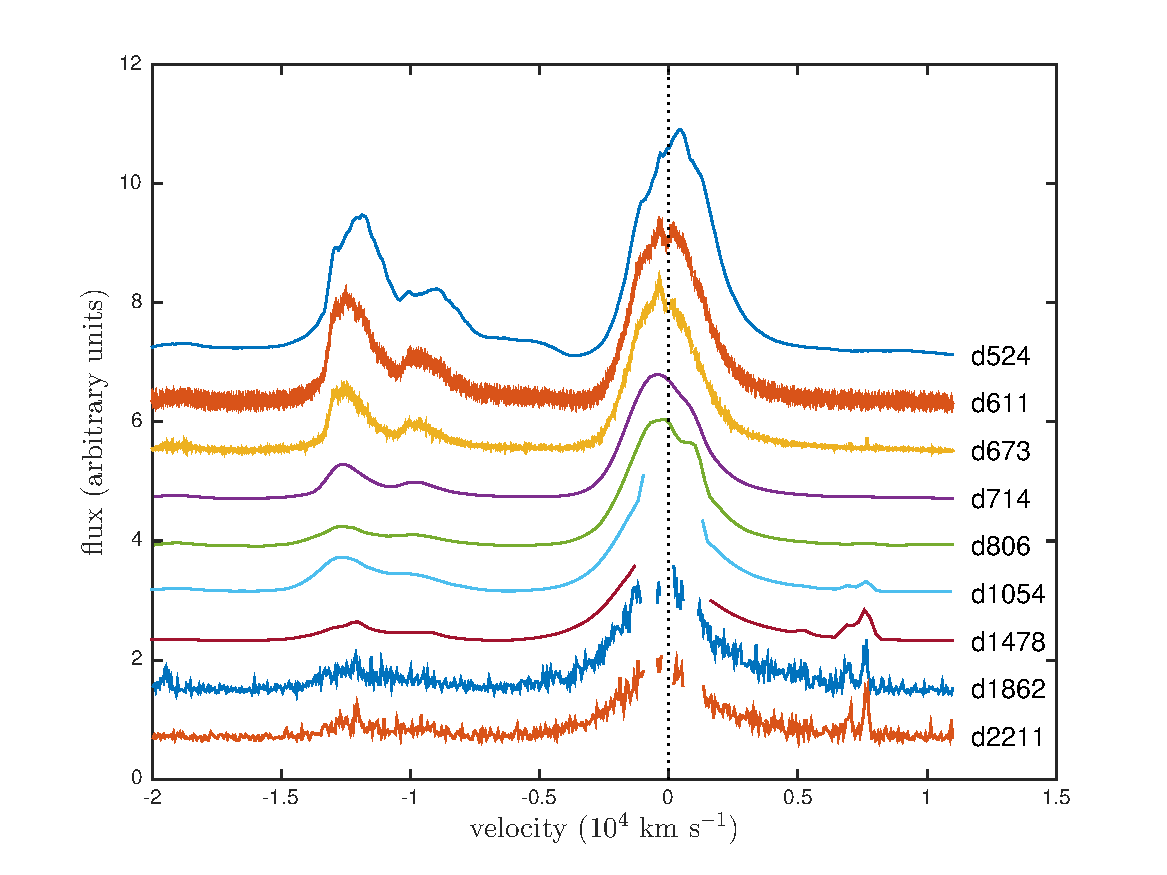
\includegraphics[trim =39 10 45 15,clip=true,scale=0.8]{chapters/chapter5/images/Ha_evol_early_1col2.pdf}
\caption{Archival data showing the evolution of the H$\alpha$ and
[O~{\sc i}] line profiles from SN~1987A at the earlier of the epochs considered. The 
spectral gaps at the last two epochs correspond to where narrow line 
emission from the equatorial ring has been removed. The spectra have been
continuum-subtracted and offsets have ben applied for display purposes.}
\label{Ha_evol_early}
%\end{center}
\end{figure}


Wavelength ranges encompassing the H$\alpha$ line and [O~{\sc 
i}]~$\lambda$6300,6363~\AA\ doublet were selected in order to trace their 
evolution from day 524, near the time of the first indications of dust 
formation \citep{Wooden1993}, to day 8020, near the current era. Optical 
spectroscopy obtained at the AAT using the Faint Object Red Spectrogaph 
(FORS) during the first two years after outburst was kindly supplied by Dr 
Raylee Stathakis \citep{Spyromilio1991, Spyromilio1993, Hanuschik1993} and 
optical spectra from the CTIO were donated by Dr Mark Phillips 
\citep{Suntzeff1991}.

The evolution of the H$\alpha$ and [O~{\sc i}] line profiles is presented 
in Figures \ref{Ha_evol_early} and \ref{Ha_evol_late}.  At later epochs, 
the broad H$\alpha$ profile emitted by the ejecta becomes contaminated by 
narrow line emission from the equatorial ring.  These lines have been 
removed for the purposes of modelling the broad line. A continuum fit has 
been subtracted from each spectrum and a velocity correction has been 
applied for a recession velocity of 287 km~s$^{-1}$ 
\citep{Groningsson2008}.

\begin{figure}
\centering
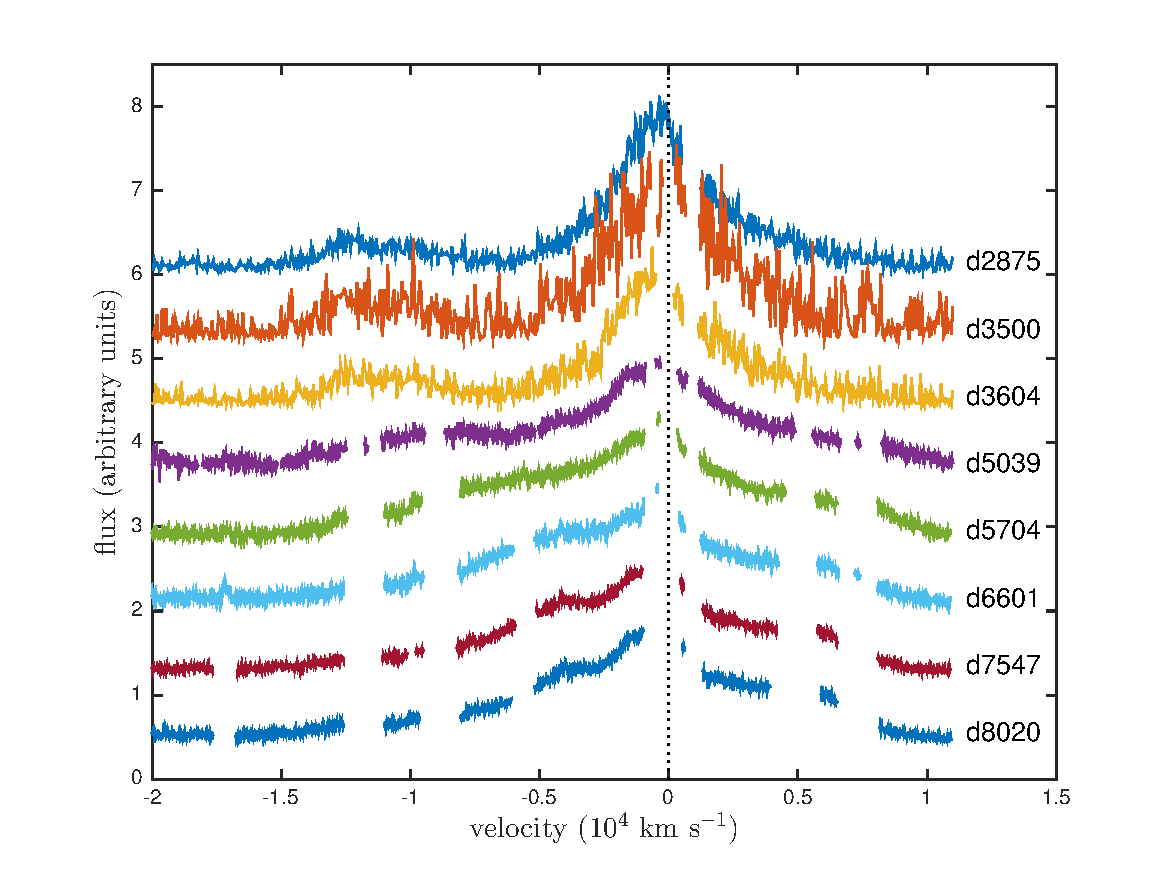
\includegraphics[trim =45 10 45 15,clip=true,scale=0.8]{chapters/chapter5/images/Ha_evol_late_1col.pdf}
\caption{Archival data showing the evolution of the H$\alpha$
line profile from SN~1987A at the later epochs. The spectral gaps 
correspond to where narrow line emission from the equatorial ring has been 
removed. The spectra have been continuum-subtracted and offsets applied 
for display purposes.}
\label{Ha_evol_late}
%\end{center}
\end{figure}
%FIGURE


\subsection{Contamination of the H$\alpha$ profiles}

The H$\alpha$ profile at day 714 exhibits a very slight inflection visible 
at $V \approx +900$ km~s$^{-1}$.  By day 806, this slight inflection has 
developed into a noticeable shoulder in the line profile of H$\alpha$ (see 
Figure \ref{Ha}).

\setlength{\tabcolsep}{5pt}
\begin{landscape}
\begin{table*}[hbtp]
	\begin{minipage}{180mm}
	\caption{Details of the archival data for SN 1987A.}
	\label{tb:data}
  	\begin{tabular}{@{} ccccccccl @{}}
    	\hline
	Date & Age & Telescope  & Inst & $\lambda_{min}$ & $\lambda_{max}$ & Res. & Res. & Reference \\
	& (days) & & &(\AA) & (\AA)& (\AA) & Power\\
	\hline
31 Jul 1988 & 524 & AAT & FORS & 5500 & 10190 & 20 & & \citet{Spyromilio1991} \\
26 Oct 1988 & 611 & AAT & UCLES & 6011 & 7336 &  & 30000 & \citet{Hanuschik1993, Spyromilio1993}\\
27 Dec 1988 & 673 & AAT & UCLES & 5702 & 10190 &  & 30000 & \citet{Hanuschik1993, Spyromilio1993}\\
06 Feb 1989 & 714 & CTIO-1.5m & Cass. & 6420 & 10380 & 16 & & \citet{Phillips1990}\\
09 May 1989 & 806 & CTIO-1.5m & Cass. & 6430 & 10330 & 16 & & \citet{Phillips1990}\\
12 Jan 1990 & 1054 & CTIO-4m & RC & 3565 & 10000 & 11 & & \cite{Suntzeff1991} \\
12 Mar 1991 & 1478 & CTIO-4m & RC & 3245 & 9175 & 11 & & \\
30 Mar 1992 & 1862 & HST & STIS & 4569 & 6818 & 4.4 &  & \citet{Wang1996}\\
14 Mar 1993 & 2211 & HST & STIS & 4569 & 6818 & 4.4 &  & \citet{Wang1996}\\
07 Jan 1995 & 2875 & HST & STIS & 4569 & 6818 & 4.4 &  & \citet{Chugai1997}\\
23 Sep 1996 & 3500 & HST & STIS & 4569 & 6818 & 4.4 &  \\ 
05 Jan 1997 & 3604 & HST & STIS & 4569 & 6818 & 4.4 &  \\
10 Dec 2000 & 5039 & VLT & UVES & 4760 & 6840 &  & 50000 & \citet{Groeningsson2006, Groeningsson2007}\\
06 Oct 2002 & 5704 & VLT & UVES & 4760 & 6840 &  & 50000 & \citet{Groeningsson2006, Groeningsson2007, Groningsson2008}\\
21 Mar 2005 & 6601 & VLT & UVES & 4760 & 6840 &  & 50000 &\citet{Groeningsson2006, Groeningsson2007}\\
23 Oct 2007 & 7547 & VLT & UVES & 4760 & 6840 &  & 50000 & \citet{Groeningsson2007}\\
07 Feb 2009 & 8020 & VLT & UVES & 4800 & 6800 &  & 50000 & \citet{Tziamtzis2010}\\
    \hline
  \end{tabular}
\end{minipage}
\end{table*}
\end{landscape}
\setlength{\tabcolsep}{12pt}


Although these features are similar in nature to features produced by dust 
absorption in the flat-topped region (as discussed in Section \ref{beta}), 
I conclude that this shoulder is an early appearance of the unresolved 
[NII] $\lambda$6583~\AA\ line from the equatorial ring \citep{Kozma1998b}.  Unresolved nebular [N~{\sc ii}] lines at $\lambda=$ 6583~\AA\ and 
$\lambda=$ 6548~\AA\ either side of the H$\alpha$ rest frame velocity at 
6563~\AA\ are certainly seen by day 1054 
%(see Figure \ref{d1054}) 
and have to be removed in order to consider the evolution of the broad 
H$\alpha$ profile (see Figure \ref{Ha_evol_early}). I do not remove this 
potential contaminant at earlier epochs but try to fit the broad line 
profiles around it.





 
By day 1054, all three of the narrow nebular lines are strong.  They 
remain unresolved in the low spectral resolution CTIO data at days 1054 
and 1478 and therefore contaminate the entire central region of the 
H$\alpha$ line profile.  Their presence renders two CTIO H$\alpha$ 
profiles from days 1054 and 1478 unusable for modelling purposes.  The HST 
and VLT H$\alpha$ profiles at later epochs ($\ge$ 1862 days) have a higher 
spectral resolution and it was therefore easier to remove the narrower 
[N~{\sc ii}] and H$\alpha$ lines from the broad H$\alpha$ profiles (for 
example Figures \ref{Ha_evol_early} and \ref{Ha_evol_late}). Although this 
does remove a potentially informative section of the profile ($+500$ 
km~s$^{-1}<v<+1500$ km~s$^{-1}$), I achieve good fits to the overall line 
profiles at these epochs.

\begin{table}
\centering
\caption{H$\alpha$ full-width half-maxima (FWHM) and the half-width zero 
intensities (HWZI) determined by the zero intensity velocity on the 
blue side of the line.  The tabulated line widths have been corrected for the relevant instrumental resolution.}
\begin{tabular}{c cc}
day & FWHM (\AA) & HWZI (\AA) \\
\hline
524 & 3200 & 3600 \\
611 & 2700 & 3400 \\
673 & 1600 & 3700 \\
714 & 3100 & 4500 \\
806 & 3200 & 5500 \\
1054 & 2100 & 5600 \\
1478 & 1400 & 6600 \\
1862 & 1600 & 6800 \\
2211 & 1400 & 6700 \\
2875 & 2700 & 6700 \\
3500 & 3500 & 7000 \\
3604 & 2100 & 7000

\end{tabular}

\label{FWHM}
\end{table}%

\subsection{The evolution of the maximum and minimum velocities}

For a freely expanding medium, the velocity of any fractional radial 
element should not change with time.  The maximum velocity of any 
line-emitting region is therefore expected to be constant.  However, at 
the epochs I consider here, it appears that the maximum velocities of the 
H$\alpha$ line, as determined by the velocity at zero intensity on the 
blue side, generally increase over time (see Table \ref{FWHM}).  I 
attribute this to the start of the freeze-out phase in the outer regions 
of the ejecta, while the hydrogen neutral fraction is still increasing in 
the denser inner regions \citep{Danziger1991,Fransson1993}.

The onset of a fixed ionization structure in the ejecta causes the rate of 
H$\alpha$ flux decline to slow.  Since the outer, faster moving regions 
reach this state at earlier times than the inner, slower moving regions, 
the relative flux contribution of the outer regions is increased.  At 
early epochs ($t<900$ days) the flux contribution from hydrogen in the 
core dominates the overall H$\alpha$ flux, whereas at later epochs ($t > 
900$ days) the flux from the envelope dominates \citep{Fransson1993, 
Kozma1998a}.  This shift likely explains apparent broadening of the line 
with the higher velocity material becoming increasingly noticeable in the 
line profiles.  This may also explain the increase in HWZI velocities at 
these epochs with the relative flux from the very densest regions dropping 
more rapidly relative to the outer line-emitting region. The full-width 
half maximum (FWHM) remains relatively steady (see Table 
\ref{FWHM}). However, the FWHM values presented in Table \ref{FWHM} were difficult 
to determine accurately since the peak of the broad line profile is 
contaminated by narrow line emission from the equatorial ring.

%%%%%%%%%%%%%%%%%%%%   SPECTRA   %%%%%%%%%%%%%%%%%%%%%%%%%%%

\section{Modelling SN~1987A}
\label{results}
\begin{figure}
\centering
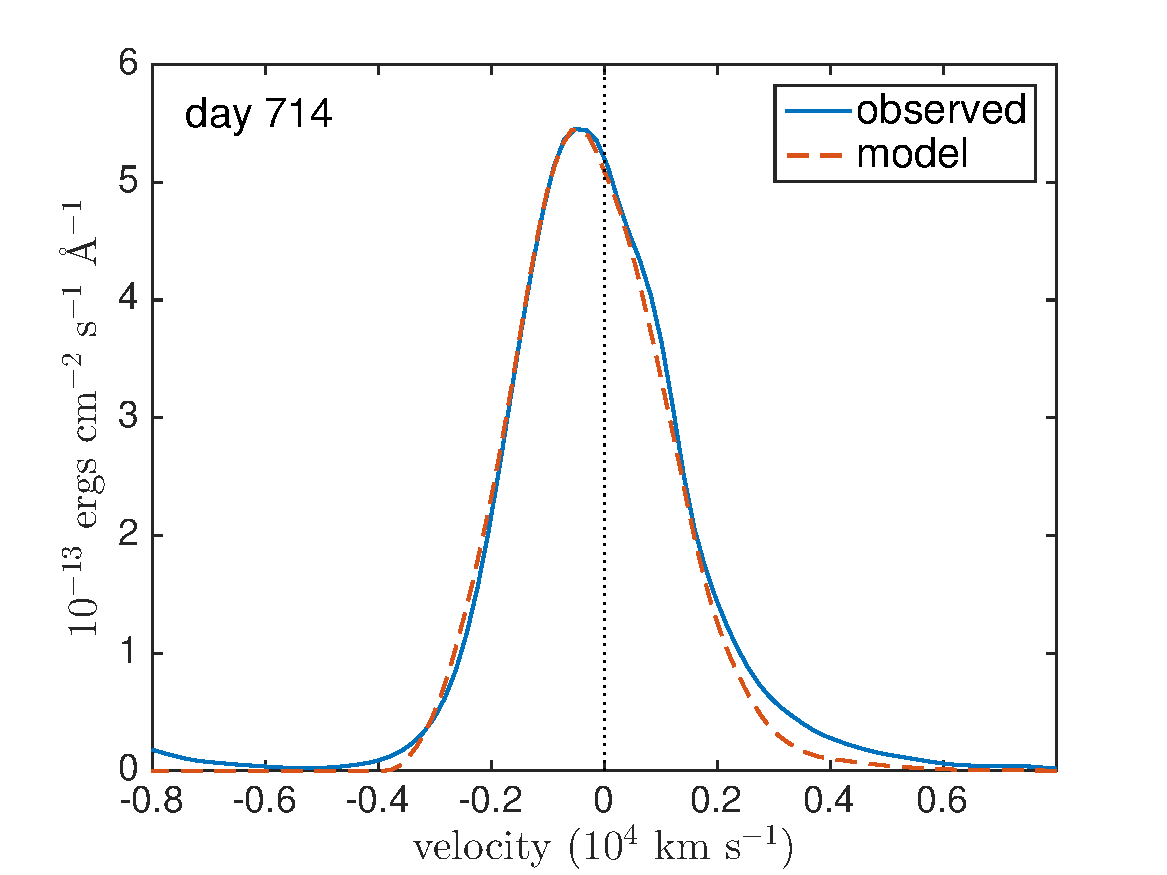
\includegraphics[trim =33 10 45 15,clip=true,scale=0.7]{chapters/chapter5/images/smooth/d714Ha_smooth_amC_MRN.pdf}
\caption{Amorphous carbon smooth dust fit to the day 714 H$\alpha$ 
line of SN~1987A using an MRN size distribution,
illustrating the underestimation of the red scattering wing for small 
grain radii.  Model parameters are the same as the smooth dust fit for 
day 714 (Table \ref{smooth1}) except for the 
grain size distribution and dust mass:  $M_{dust}=8.0 \times 10^{-6} 
M_{\odot}$, $a_{min}=0.005~\mu$m, $a_{max}=0.25~\mu$m and $n(a) \propto 
a^{-3.5}$.}
\label{MRN}

\end{figure}

\begin{figure*}
\centering
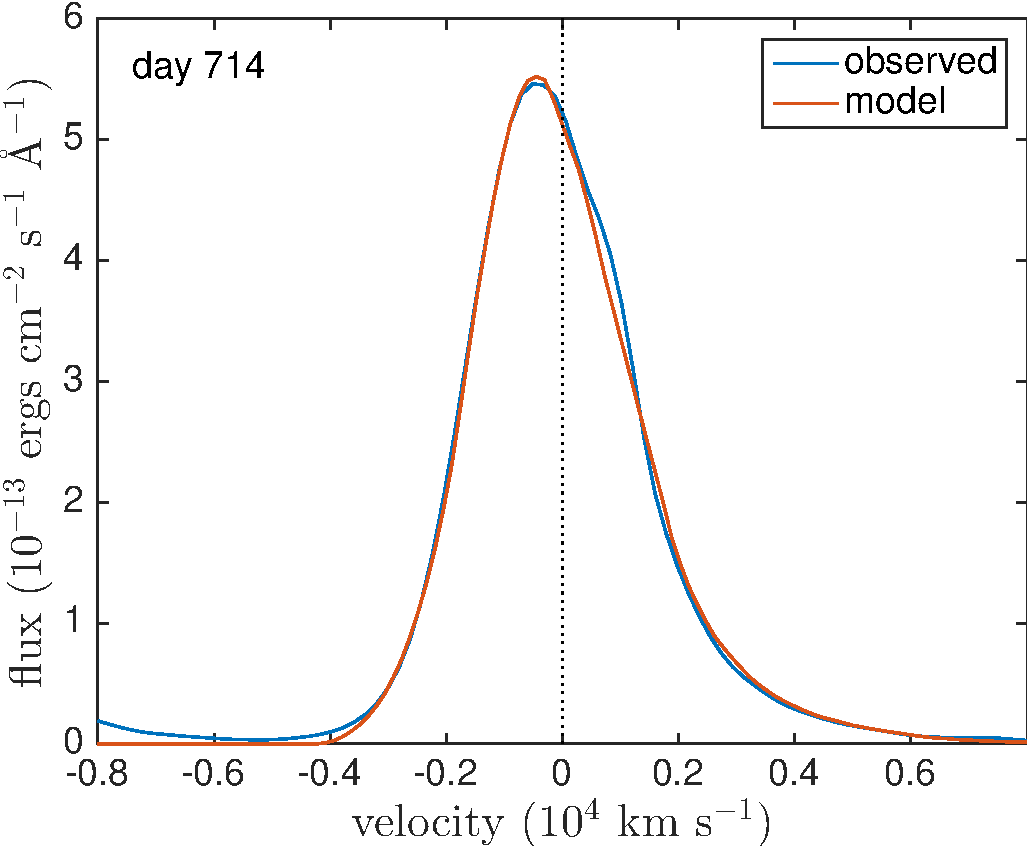
\includegraphics[trim =0 0 0 0,clip=true,scale=0.4]{chapters/chapter5/images/smooth/best_fit/d714Ha_new.pdf}
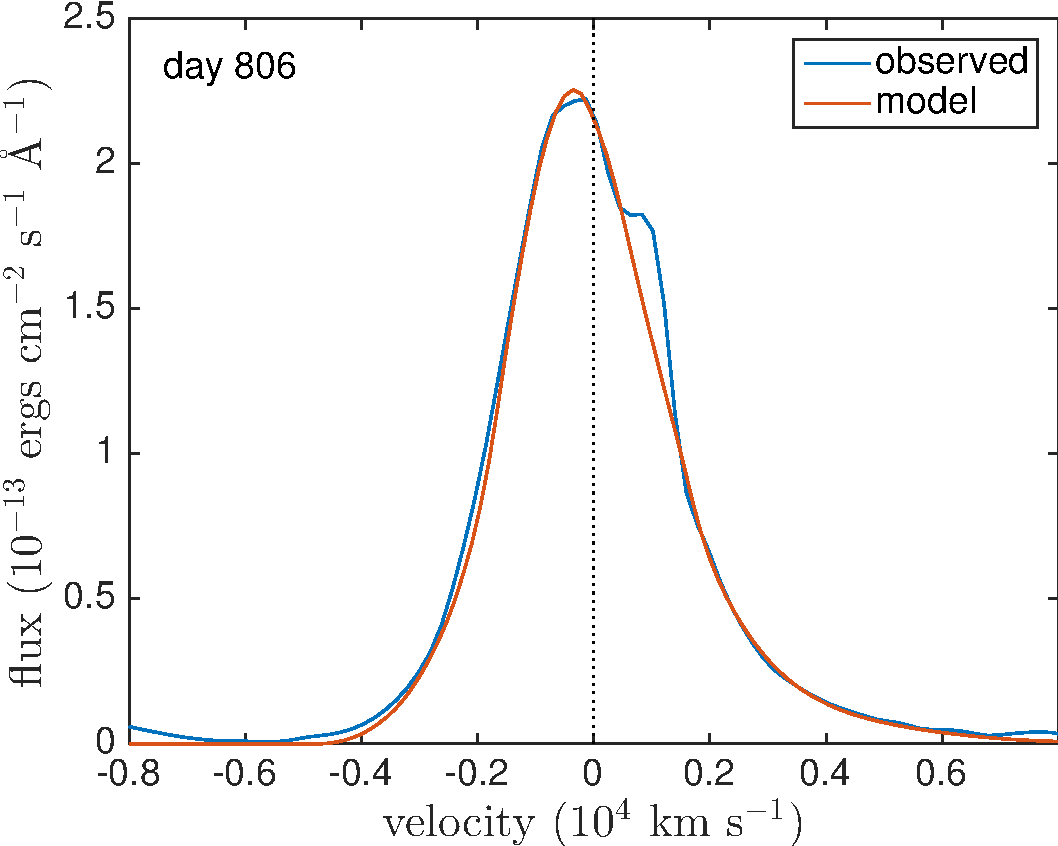
\includegraphics[trim =25 0 0 0,clip=true,scale=0.4]{chapters/chapter5/images/smooth/best_fit/d806Ha_new.pdf}

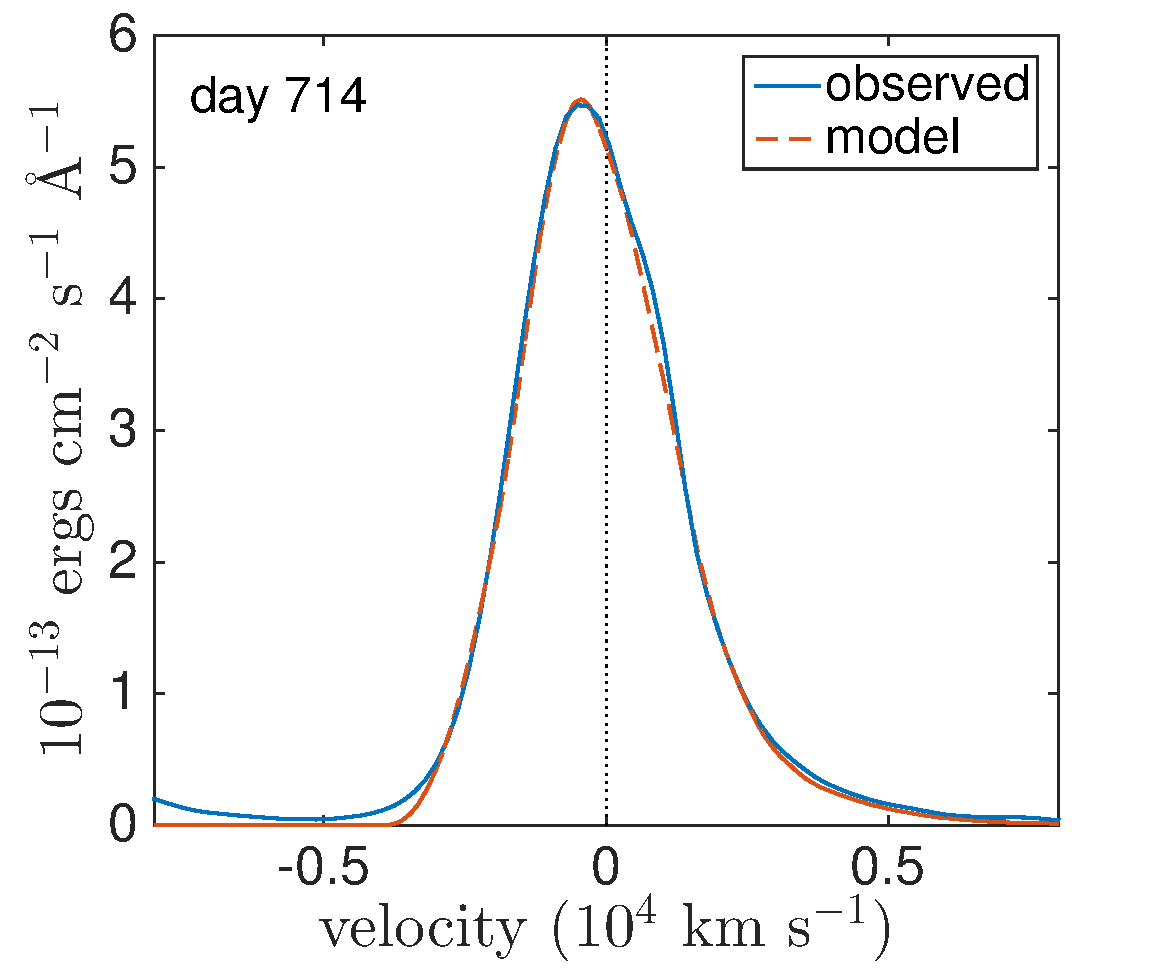
\includegraphics[trim =25 0 0 0,clip=true,scale=0.4]{chapters/chapter5/images/clump_1/best_fit/d714Ha_new.pdf}
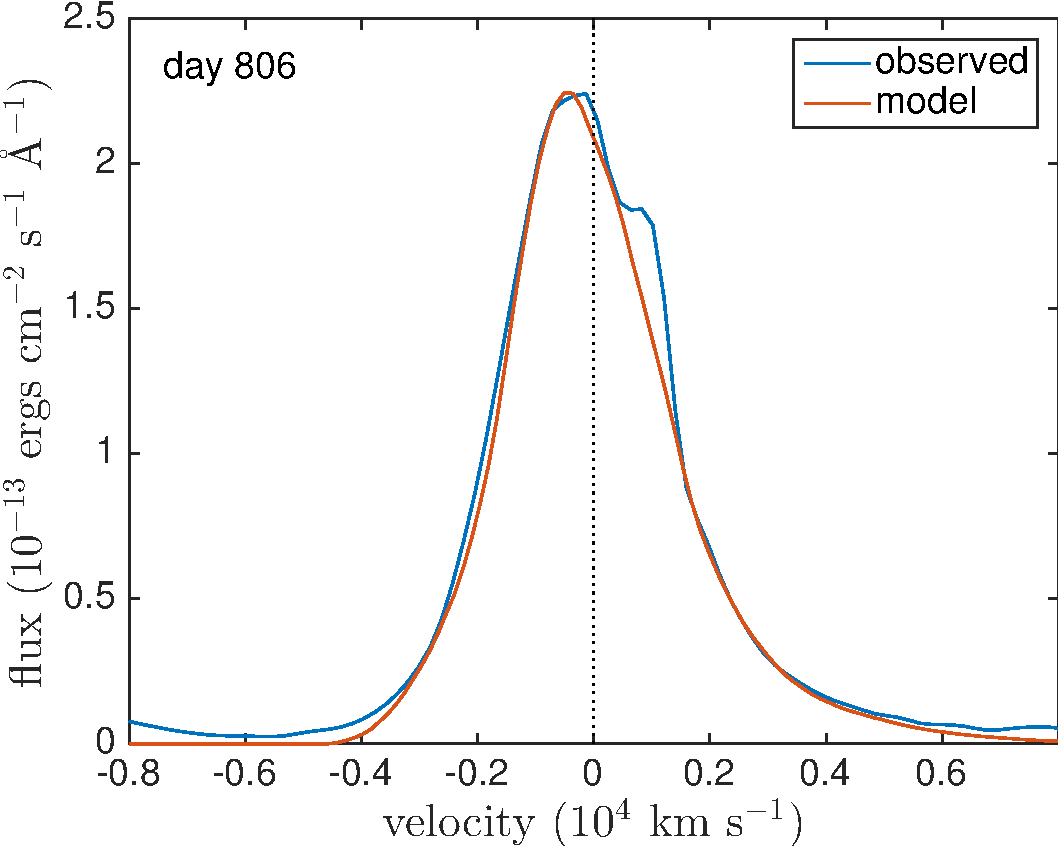
\includegraphics[trim =25 0 0 0,clip=true,scale=0.4]{chapters/chapter5/images/clump_1/best_fit/d806Ha_new.pdf}
\caption{Best model fits to the SN~1987A H$\alpha$ line at day 714 
and day 806 for the parameters detailed in Tables \ref{smooth1} and \ref{clumped1}. The two fits on the top are smooth dust models using amorphous carbon grains of radius $a=0.35~\mu$m and the two fits on the bottom are clumped dust models using amophous carbon grains of radius $a=0.6~\mu$m.}
\label{Ha}

\end{figure*}


I have modelled the H$\alpha$ line of SN~1987A at days 714, 806, 1862, 
2211, 2875, 3500 and 3604, and the [O~{\sc i}]~$\lambda$6300,6363~\AA\ 
doublet at days 714, 806, 1054 and 1478.  After day 3604 the H$\alpha$ 
profile begins to become dominated by emission from the reverse shock and 
the structure of the emitting region may no longer be approximated by a 
single shell model as I do here \citep{Fransson2013}.  The [O~{\sc 
i}]~$\lambda$6300,6363~\AA\ doublet becomes too weak to model after day 
1478 (see Figure \ref{Ha_evol_early}).  I continue to adopt a velocity 
profile $V(r) = \frac{V_{max}}{R_{max}}r$ and treat the variable 
parameters listed at the start of Section \ref{ps}.  Whilst the albedo and 
optical depth are not varied directly, they are altered by adjusting the 
dust mass, $M_{dust}$, and the grain size, $a$, which together determine 
the albedo and optical depth via Mie theory and the optical properties of 
the dust.

\setlength{\tabcolsep}{10pt}
\begin{table}
\caption{Observed luminosities of the H$\alpha$ line and estimated 
electron scattering optical depths from $R_{in}$ to $R_{out}$ for the 
radii detailed in Tables \ref{smooth1} to \ref{clumped1} based on an 
assumed gas temperature of 10,000~K.}
\centering
\begin{tabular}{@{}cccccc@{}}
\hline
& \multicolumn{2}{c}{H$\alpha$} &  \multicolumn{2}{c}{[O~{\sc i}]}  \\
day &  $L_{obs}$ & $L_{undep}$/  &  $L_{obs}$ & $L_{undep}$/   & $\tau_e$ \\
& (10$^{37}$ erg s$^{-1}$) &$L_{obs}$& (10$^{37}$ erg s$^{-1}$) & $L_{obs}$& ($10^{-2}$) \\
\hline
714 & 1.36 & 1.65 &0.313&3.57& 1.44  \\
806 & 0.57 & 1.77 &0.0942&3.57& 0.840 \\
1054 &&&0.0242 & 3.23\\
1478 &&& 0.00185&2.70 \\
1862 & 0.0063 & 2.06 &&& 0.159  \\
2211 & 0.0041 & 2.07 &&& 0.0378  \\
2875 & 0.0019 & 2.84 & & &0.0219  \\
3500 & 0.00079 & 3.16 & &&0.0125  \\
3604 & 0.00098 & 3.27 &&&0.0149  \\

\hline
\end{tabular}

\label{tau_e}
\end{table}%
\setlength{\tabcolsep}{8pt}


In all models, the ejecta occupies a shell with inner radius $R_{in}$ and 
outer radius $R_{out}$.  Packets are emitted according to a smooth density 
profile assuming recombination or collisional excitation such that $i(r) 
\propto \rho(r)^2 \propto r^{-2\beta}$.  Initially the dust is considered 
to have a smooth density distribution and is assumed to be coupled to the 
gas so as to follow the same radial profile.  A clumped distribution of 
dust is considered later (see Section \ref{clumped_models}).

Assuming an electron temperature of 10,000~K, I estimated the total electron scattering optical depths between $R_{in}$ and $R_{out}$ based on the 
observed fluxes of the H$\alpha$ recombination line. A temperature of 10,000~K for the recombining material is 
likely too high at the epochs considered but I adopt it in order
not to underestimate electron scattering optical depths.  The values 
I calculate from the observed H$\alpha$ luminosities are listed in Table 
\ref{tau_e}.  Since the electron scattering optical depths at these epochs 
are negligibly small I therefore do not include electron scattering in 
the models.




There is rarely a unique set of parameters that provide the best fit to 
the data.  However, the majority of the parameters of interest can be well 
constrained from my modelling by considering different elements of the 
shape of the profile.  In particular, by constructing fits to the data 
using minimum and maximum limits for the grain radius, credible lower and 
upper bounds on the dust mass formed within the ejecta may be derived.  
I present here fits to the data obtained using both small and large 
values of the grain radius $a$ since it is the grain size which has the 
most significant effect on the overall dust mass required to reproduce the 
line profile (see Section \ref{params}).


All of my models are of a dusty medium composed solely of amorphous 
carbon grains. I use the optical constants from the BE sample presented 
by \citet{Zubko1996}.  Although previous SED modelling of SN~1987A  
limited the fraction of silicates present in the dusty ejecta to a maximum 
of 15\% (\citet{Ercolano2007}, W15), the recent work of \citet{Dwek2015} has suggested that a large mass of mostly silicate dust may have formed at early epochs ($\sim$ 615 days).  It is therefore useful to consider the effects 
on my models of using silicate dust.  I discuss this in detail in 
Sections \ref{species} and \ref{dwek}.

For each profile, the maximum velocity is initially identified from the 
data as the point where the emission vanishes on the blue side and is then 
varied throughout the modelling in order to produce the best fit.  The 
equivalent point on the red side is indeterminate from observations due to 
the effects of dust scattering.  I determine the approximate value of 
$V_{min}$ by examining the width of the profile near its peak. On the red side the theoretical minimum velocity often 
falls at a similar velocity to the 6583\AA\ line so any dust-induced 
features near this wavelength that would allow a more accurate 
determination of $V_{min}$ can be overwhelmed by the nebular line.  
Having determined the minimum and maximum velocities, the ratio of the 
inner and outer radii of the supernova ejecta can be determined since 
$R_{in}/R_{out}=V_{min}/V_{max}$.  The outer radius is calculated from the 
epoch and the maximum velocity.

The only parameters that  remain to be determined are the exponent of 
the density profile $\beta$, the mean grain radius and the total dust 
mass.  The shape of the blue wing is solely a product of the density 
profile and the dust mass; the height and shape of the red wing is a 
product of these and also of the scattering efficiency of the grains (the 
albedo $\omega$); the extent and shape of the asymmetry in the flat-topped 
portion of the profile is a function of only the total dust optical depth 
determined by the dust mass and the grain radius.  By iterating over these 
three parameters, an excellent fit to the data can usually be 
obtained.

Models are produced in the same manner for the [O~{\sc 
i}]~$\lambda$6300,6363~\AA\ doublet as for the single H$\alpha$ line, with 
each component of the doublet being modelled independently and the 
resulting profiles added according to a specified ratio.  Although the 
theoretical intrinsic flux ratio is 3.1 for optically thin emission \citep{Storey2000}, the 
actual ratio between the two components can be affected by self-absorption 
\citep{Li1992} and I therefore left it as a free parameter.  The deduced 
doublet ratios are listed in Tables \ref{smooth1}, \ref{clumped1} and 
\ref{clumped2}.


\begin{figure*}
\centering
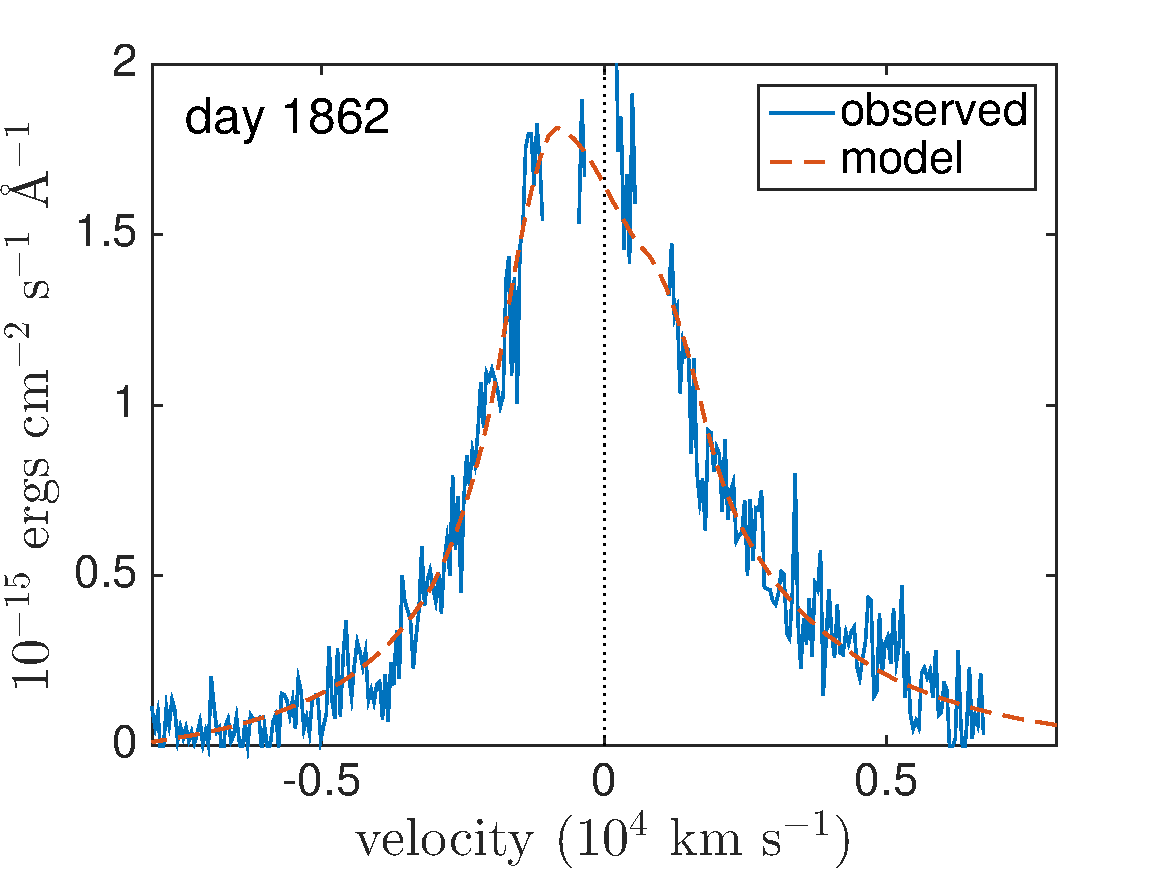
\includegraphics[trim =0 0 0 0,clip=true,scale=0.4]{chapters/chapter5/images/smooth/best_fit/d1862Ha.pdf}
\hspace{2mm}
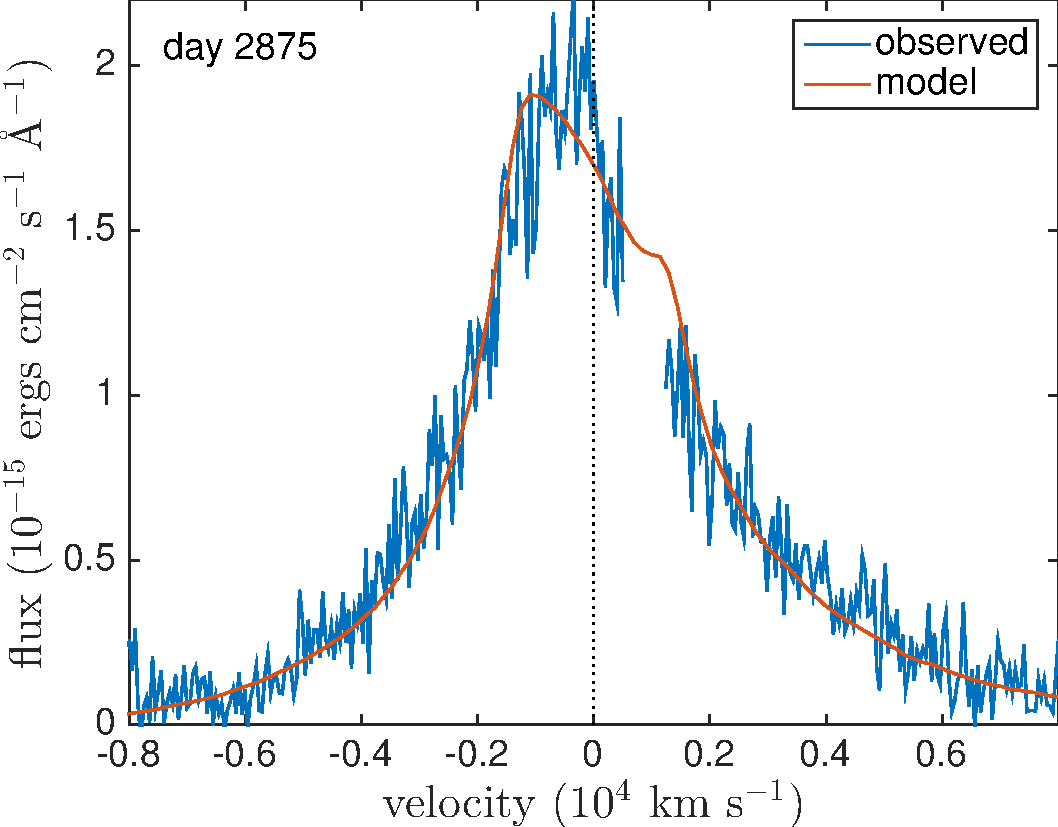
\includegraphics[trim =25 0 0 0,clip=true,scale=0.4]{chapters/chapter5/images/smooth/best_fit/d2875Ha.pdf}

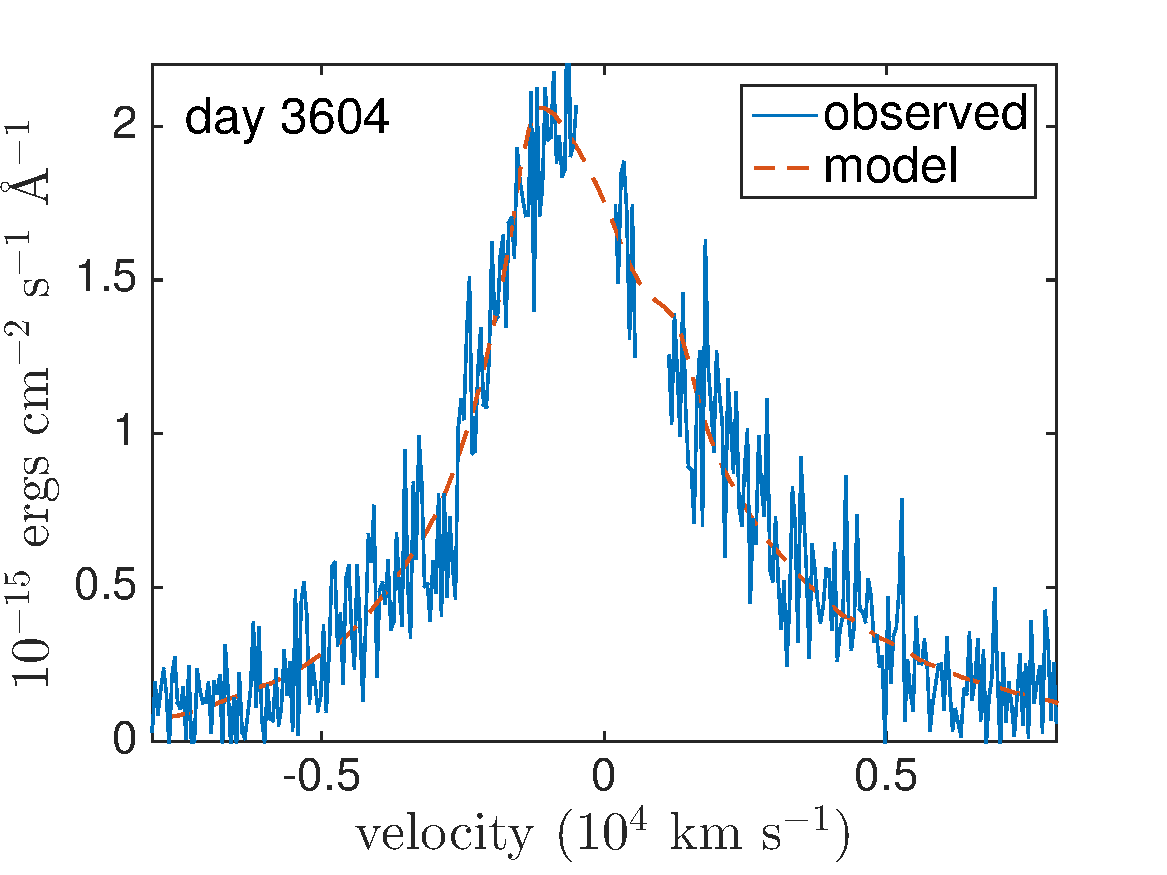
\includegraphics[trim =0 0 0 -30,clip=true,scale=0.4]{chapters/chapter5/images/smooth/best_fit/d3604Ha.pdf}
\caption{Best model fits to the SN~1987A H$\alpha$ line at days 1862, 2875 and 
3604 for the parameters detailed in Tables \ref{smooth1}, \ref{clumped1} and \ref{clumped2}.  On the top row are smooth model fits with amorphous carbon grains of radius $a=0.35~\mu$m.  On the middle and bottom rows are clumped model fits with amorphous carbon grains of radii $a=0.6~\mu$m and $a=3.5~\mu$m respectively.}
\label{}
\end{figure*}

\begin{figure*}
\centering
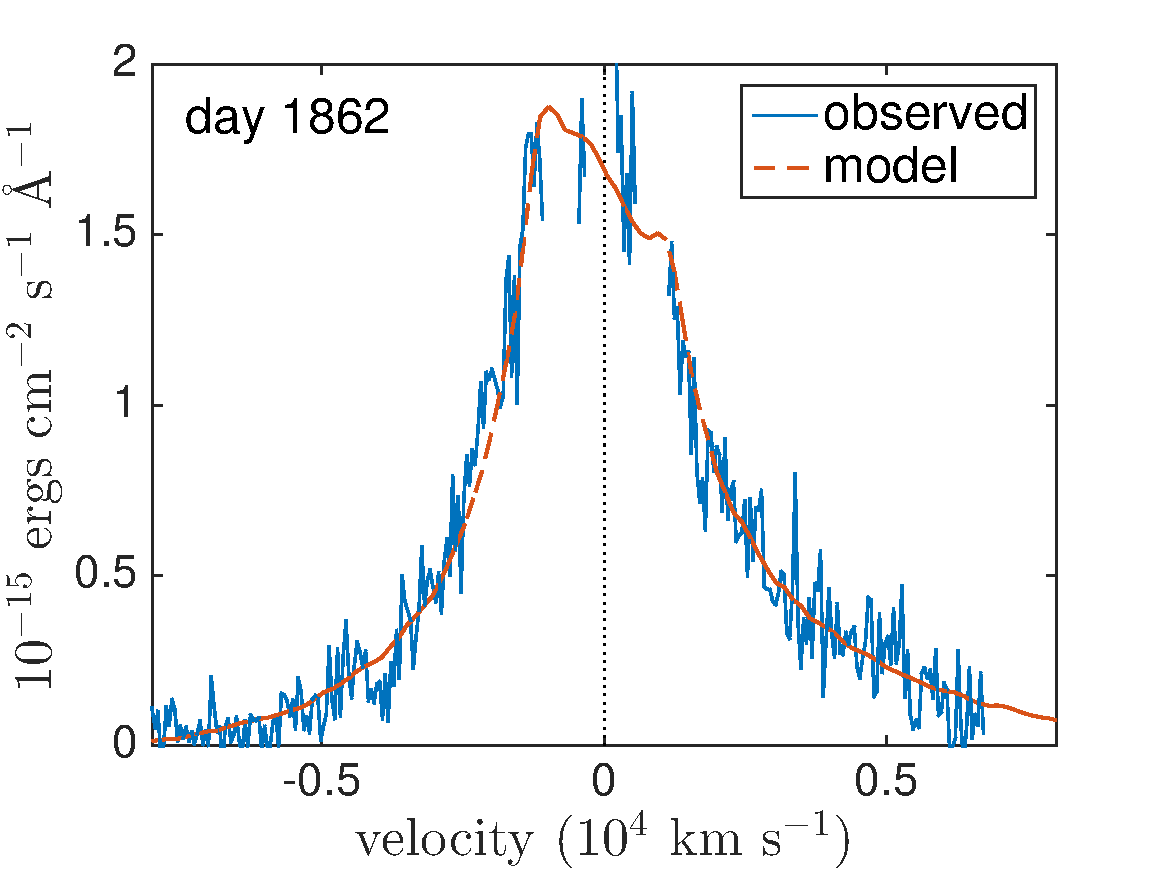
\includegraphics[trim =0 25 0 -20,clip=true,scale=0.4]{chapters/chapter5/images/clump_1/best_fit/d1862Ha.pdf}
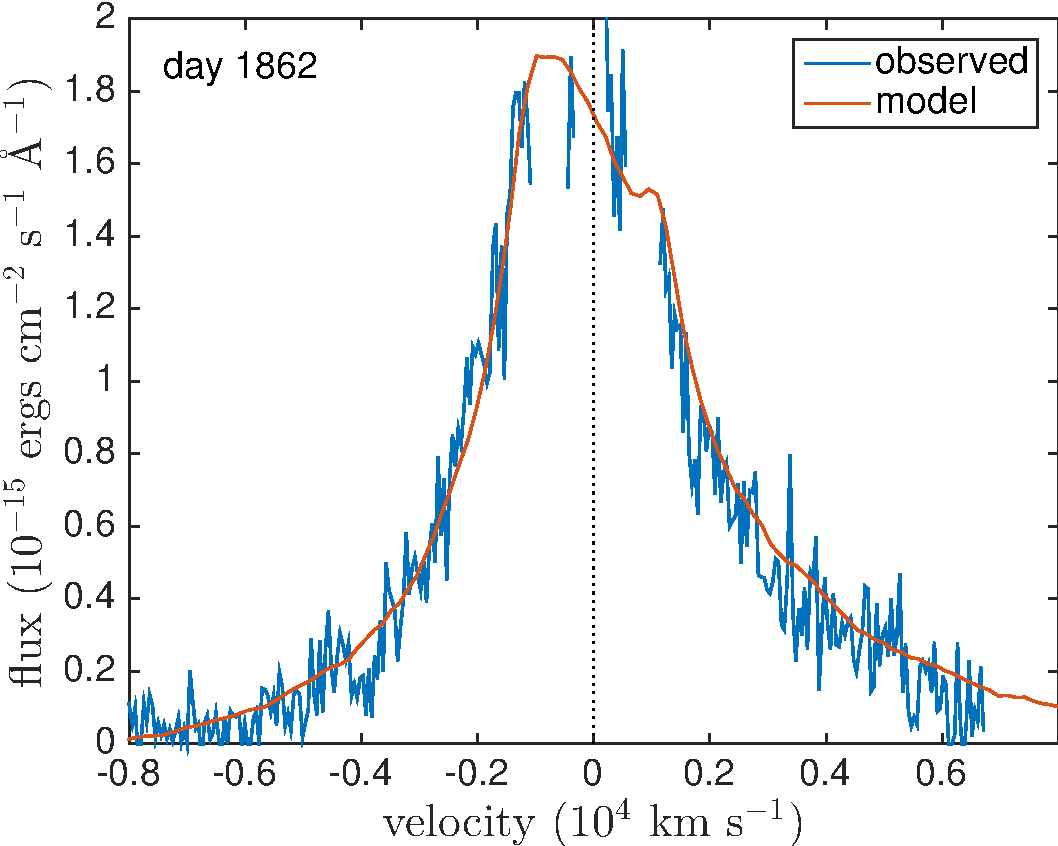
\includegraphics[trim =25 25 0 -20,clip=true,scale=0.4]{chapters/chapter5/images/clump_1/maximum/d1862Ha.pdf}

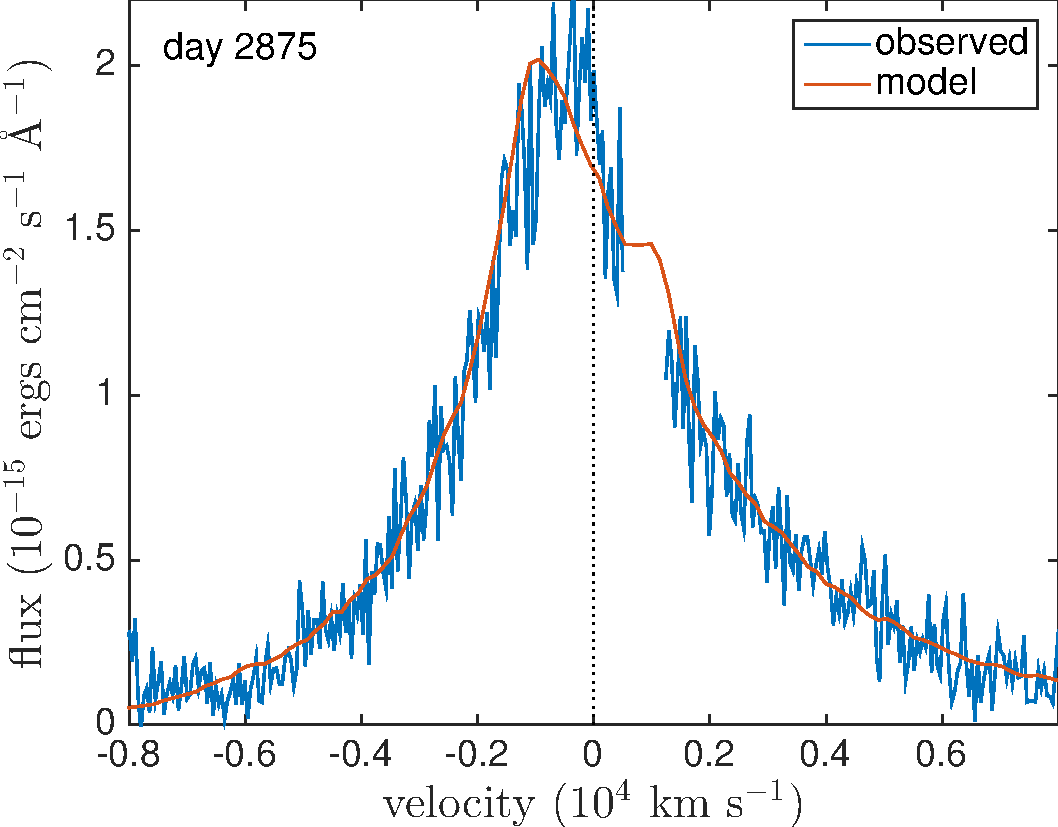
\includegraphics[trim =0 25 0 -20 ,clip=true,scale=0.4]{chapters/chapter5/images/clump_1/best_fit/d2875Ha.pdf}
\includegraphics[trim =25 25 0 -20,clip=true,scale=0.4]{chapters/chapter5/images/clump_1/maximum/d2875Ha.pdf}

\includegraphics[trim =0 0 0 -20,clip=true,scale=0.4]{chapters/chapter5/images/clump_1/best_fit/d3604Ha.pdf}
\includegraphics[trim =25 0 0 -20,clip=true,scale=0.4]{chapters/chapter5/images/clump_1/maximum/d3604Ha.pdf}
\vspace{8mm}
\caption{Best model fits to the SN~1987A H$\alpha$ line at days 1862, 2875 and 
3604 for the parameters detailed in Tables \ref{smooth1}, \ref{clumped1} and \ref{clumped2}.  On the top row are smooth model fits with amorphous carbon grains of radius $a=0.35~\mu$m.  On the middle and bottom rows are clumped model fits with amorphous carbon grains of radii $a=0.6~\mu$m and $a=3.5~\mu$m respectively.}
\label{d1862_3604}

\end{figure*}

For all lines, though particularly at very late epochs, even small 
fluctuations in the adopted value of the continuum level can have a 
substantial effect on the fit to the resulting profile.  Since it is not 
feasible to establish the level of the continuum so precisely, the value 
of the continuum has been left as a free parameter that may be adjusted 
(to within sensible margins) in order to allow for the widest possible 
dust mass range to be determined.  I generally find it is necessary to 
assume a continuum level that is slightly lower where the dust mass is 
higher.  The [O~{\sc i}]$\lambda$6300,6363~\AA\ doublets at days 1054 and 
1478 are weak relative to the continuum and are also blended with the 
wings of other lines making it difficult to fit their wings accurately.  
I aim to fit the lines between approximately -3000 km s$^{-1}$ and +5000 
km s$^{-1}$ but present a wider velocity range for context (for example 
see Figure \ref{OI_smooth}).


Fits to the H$\alpha$ line profile at days 2211 and 3500 are omitted for 
the sake of space but are very similar to those of days 1862 to 3604.  
All profiles have been smoothed to approximately the same resolution as 
the observed profiles using a moving-average procedure.  Parameters for 
the models at all epochs including days 2211 and 3500 are detailed in 
Tables \ref{smooth1} to \ref{clumped2}.


\subsection{Smooth Density Models for SN 1987A}
\label{smooth_models}

Even at the earliest epochs there is a substantial wing on the red side of 
the H$\alpha$ line profile that cannot be fitted by scattering from moving 
grains with a low albedo.  The minimum required albedo is approximately 
$\omega \approx 0.5$ implying relatively large grain radii.  As previously 
discussed, the larger the grain size the larger the mass of dust required 
to reproduce the same optical depth.  Figure \ref{MRN} illustrates the fit 
for the day 714 H$\alpha$ profile for the case where a classic MRN 
\citep{Mathis1977} grain size distribution is adopted, with $a_{min}=0.005 
\mu$m, $a_{max}=0.25~\mu$m and $n(a) \propto a^{-3.5}$.  It can be seen 
clearly that the extended red wing is significantly underestimated.  
Since the albedo of amorphous carbon grains varies significantly with 
grain radius (see Figure \ref{albedo_grain}) I can establish a strong 
lower bound to the mean dust grain radius, which I estimate to be $a \ge 
0.35~\mu$m.  This is the smallest grain size that is still capable of 
reproducing the red scattering wing at all epochs and I therefore use 
this lower limit value throughout my smooth density modelling.


The inner and outer radii of the ejecta are calculated at each epoch from 
the maximum velocity used, the day number and the specified ratio 
$R_{in}/R_{out}$.  The radii generated are consistent with those used in 
previous models of SN 1987A (\citet{Ercolano2007}, W15) and the 
minimum velocities for both the [O~{\sc i}] and H$\alpha$ line emitting 
regions are relatively consistent with those obtained by \citet{Kozma1998b} 
who estimate that  hydrogen extends into the core to a depth of 
$\lesssim 700$~km~s$^{-1}$ and the oxygen reaches down to $\sim 
400$~km~s$^{-1}$.  They are also consistent with predictions from 3D 
explosion models at the time of shock-breakout that predict the oxygen to 
reach to a depth of $\sim 200$~km~s$^{-1}$ 
\citep{Hammer2010,Wongwathanarat2015}. Figures \ref{Ha} and 
\ref{d1862_3604} show the best fits to the data for days 714 to 3604 
whilst Table \ref{smooth1} details the parameters used.

It can be seen from Tables \ref{smooth1} to \ref{clumped2} that, in order 
to reproduce the blueshifts seen in the [O~{\sc 
i}]~$\lambda$6300,6363~\AA\ doublet, considerably larger dust masses are 
required than to fit the H$\alpha$ line at the same epoch.  Although the 
same maximum velocities and therefore outer radii are used in my [O~{\sc 
i}] and H$\alpha$ models, the inner radii for the [O~{\sc i}] models are 
significantly smaller and the density distribution much steeper.  This 
implies that [O~{\sc i}] is concentrated towards the centre of the 
ejecta whereas H$\alpha$ is more diffuse.  This is broadly in 
agreement with 3D explosion dynamics models that suggest that a few hours 
after the explosion the heavier elements will, in comparison to hydrogen, 
be located more centrally in the ejecta with ``bullets" of heavier 
material reaching the outer edges \citep{Hammer2010}.  If dust is forming 
in the inner regions of the ejecta then the majority of the [O~{\sc i}] 
emission must travel through the newly formed dust whereas the more 
diffuse H$\alpha$ emission has a greater chance of escaping unaffected.  
This may explain the difference between the dust masses needed for the 
[O~{\sc i}] and H$\alpha$ models.


\begin{landscape}

\begin{table*}
\centering
	\begin{minipage}{180mm}
	\caption{The parameters used for the best fitting 
smooth models of SN~1987A with amorphous carbon grains of radius $a=0.35~\mu$m.  Optical depths are given from $R_{in}$ to $R_{out}$ at $\lambda = 6563$~\AA\ for H$\alpha$ and $\lambda = 6300$~\AA\ for [O~{\sc i}]. Values of $\tau_V$ are very close to the quoted values of $\tau_{H\alpha}$.}
	\label{smooth1}
	\centering
  	\begin{tabular}{@{} cccccccccccc @{}}
    	\hline
 & day & $V_{max}$ & $V_{min}$ & $R_{in}/R_{out}$ & $\beta$ & $M_{dust}$ & $R_{out}$ & $R_{in}$ & [O~{\sc i}] ratio & $\tau_{\lambda}$   \\
	&& (km~s$^{-1} $)& (km~s$^{-1} $) & & & ($M_{\odot}$) & (cm) & (cm) \\
	\hline


[O~{\sc i}]  & 714 & 3250 & 228 & 0.07  & 2.9 & 9.65$\times 10^{-5}$ & 2.00$\times 10^{16}$ & 1.40$\times 10^{15}$ & 2.6 & 3.60  \\ \relax
[O~{\sc i}]  & 806 & 4000 &  240 & 0.06 & 2.4 & 1.50$\times 10^{-4}$ & 2.79$\times 10^{16}$ & 1.67$\times 10^{15}$ & 2.3 & 2.86 \\ \relax
[O~{\sc i}]  & 1054 & 4300 & 215& 0.05  & 2.1 & 2.35$\times 10^{-4}$ &   3.92$\times 10^{16}$ & 1.96$\times 10^{15}$ & 2.7 & 2.23  \\ \relax
[O~{\sc i}]  & 1478 & 4500 & 180 & 0.04  & 1.7 & 2.95$\times 10^{-4}$ &   5.75$\times 10^{16}$ & 2.30$\times 10^{15}$ & 3.0 & 1.30 \\
H$\alpha$ & 714 & 3250 & 813 & 0.25  & 1.2 & 2.10$\times 10^{-5}$ &   2.00$\times 10^{16}$ & 5.01$\times 10^{15}$ & & 0.61\\
H$\alpha$ & 806 & 4000  & 880 & 0.22 & 1.9 & 3.80$\times 10^{-5}$ &   2.79$\times 10^{16}$ & 6.13$\times 10^{15}$ & & 0.59 \\
H$\alpha$ & 1862 & 8500 &  1275 & 0.15  & 1.9 & 5.00$\times 10^{-4}$ &   1.37$\times 10^{17}$ & 2.05$\times 10^{16}$ & & 0.35\\
H$\alpha$ & 2211 & 9000 & 1260& 0.14 & 1.9 & 9.25$\times 10^{-4}$ &   1.72$\times 10^{17}$ & 2.41$\times 10^{16}$ & & 0.42\\
H$\alpha$ & 2875 & 9500 & 1330 & 0.14 & 1.9 & 1.50$\times 10^{-3}$ &   2.36$\times 10^{17}$ & 3.30$\times 10^{16}$ & & 0.36 \\

H$\alpha$ & 3500 & 10000 & 1400 & 0.14 & 1.9 & 3.35$\times 10^{-3}$  & 3.02$\times 10^{17}$ & 4.23$\times 10^{16}$ && 0.49   \\

H$\alpha$ & 3604 & 10250 & 1333 & 0.13 & 1.9 & 4.20$\times 10^{-3}$ &   3.19$\times 10^{17}$ & 4.15$\times 10^{16}$ & & 0.55 \\ 

    \hline
  \end{tabular}

\end{minipage}
\end{table*}
\end{landscape}

\begin{landscape}
\begin{table*}
\centering
	\begin{minipage}{180mm}
	\caption{The parameters used for the best fitting  
clumped models of SN~1987A with amorphous carbon grains of radius $a=0.6~\mu$m. Optical depths are given from $R_{in}$ to $R_{out}$ at $\lambda = 6563$~\AA\ for H$\alpha$ and $\lambda = 6300$~\AA\ for [O~{\sc i}]. Values of $\tau_V$ are very close to the quoted values of $\tau_{H\alpha}$.}
	\label{clumped1}
\centering
  	\begin{tabular}{@{} ccccccccccccc @{}}
    	\hline
 & day & $V_{max}$ & $V_{min}$ & $R_{in}/R_{out}$ & $\beta$ & $M_{dust}$ & $R_{out}$ & $R_{in}$ &  [O~{\sc i}] ratio & $\tau_{\lambda}$    \\
	&& (km~s$^{-1} $) & (km~s$^{-1} $)& & & ($M_{\odot}$) & (cm) & (cm)   \\
	\hline
[O~{\sc i}]  & 714 & 3250 & 228& 0.07 & 2.7 & 2.00$\times 10^{-4}$ & 2.00$\times 10^{16}$ & 1.40$\times 10^{15}$ & 2.3 & 3.84   \\ \relax
[O~{\sc i}]  & 806 & 4000 & 240&0.06 & 2.3 & 4.00$\times 10^{-4}$ & 2.79$\times 10^{16}$ & 1.67$\times 10^{15}$ & 2.0 & 4.02  \\ \relax
[O~{\sc i}]  & 1054 & 4300 & 215&0.05 & 2.3 & 7.50$\times 10^{-4}$ &   3.92$\times 10^{16}$ & 1.96$\times 10^{15}$ & 2.3 & 3.85  \\ \relax
[O~{\sc i}]  & 1478 & 4500 & 180&0.04 & 2.0 & 1.10$\times 10^{-3}$ &   5.75$\times 10^{16}$ & 2.30$\times 10^{15}$ & 2.8 & 2.65  \\
H$\alpha$ & 714 & 3250 & 813&0.25 & 1.4 & 5.50$\times 10^{-5}$ &   2.00$\times 10^{16}$ & 5.01$\times 10^{15}$ & & 0.87  \\
H$\alpha$ & 806 & 4000 & 880&0.22 & 1.8 & 9.00$\times 10^{-5}$ &   2.79$\times 10^{16}$ & 6.13$\times 10^{15}$ & & 0.76 \\
H$\alpha$ & 1862 & 8500 & 1190&0.14 & 1.9 & 1.20$\times 10^{-3}$ &   1.37$\times 10^{17}$ & 1.91$\times 10^{16}$ & & 0.46  \\

H$\alpha$ & 2211 & 9000 & 1260&0.14 & 1.9 & 3.00$\times 10^{-3}$ &   1.72$\times 10^{17}$ & 2.41$\times 10^{16}$ & & 0.73 \\

H$\alpha$ & 2875 & 9500 & 1140&0.12 & 2 & 8.00$\times 10^{-3}$ &   2.36$\times 10^{17}$ & 2.83$\times 10^{16}$ & & 1.05  \\

H$\alpha$ & 3500 & 10000 & 1200&0.12 & 2 & 1.35$\times 10^{-2}$  & 3.02$\times 10^{17}$ & 3.63$\times 10^{16}$ && 1.08   \\

H$\alpha$ & 3604 & 10250 & 1230&0.12 & 2 & 1.70$\times 10^{-2}$ &   3.19$\times 10^{17}$ & 3.83$\times 10^{16}$ & & 1.22 \\ 

    \hline
  \end{tabular}

\end{minipage}
\end{table*}
\end{landscape}

\begin{landscape}
\begin{table*}
\centering
	\begin{minipage}{180mm}
	\caption{The parameters used for the best fitting 
clumped models of SN~1987A with amorphous carbon grains of radius $a=3.5~\mu$m. Optical depths are given from $R_{in}$ to $R_{out}$ at $\lambda = 6563$~\AA\ for H$\alpha$ and $\lambda = 6300$~\AA\ for [O~{\sc i}]. Values of $\tau_V$ are very close to the quoted values of $\tau_{H\alpha}$.}
	\label{clumped2}
\centering
  	\begin{tabular}{@{} cccccccccccccc @{}}
    	\hline
 & day & $V_{max}$ & $V_{min}$ & $R_{in}/R_{out}$ & $\beta$ & $M_{dust}$  & $R_{out}$ & $R_{in}$ & [O~{\sc i}] ratio & $\tau_{\lambda}$ \\
	&& (km~s$^{-1} $) &  (km~s$^{-1} $) & & & ($M_{\odot}$)  & (cm) & (cm)  \\
	\hline
[O~{\sc i}]  & 714 & 3250 &228& 0.07 & 2.9 & 1.50$\times 10^{-3}$ & 2.00$\times 10^{16}$ & 1.40$\times 10^{15}$ & 2.3 & 4.20   \\ \relax
[O~{\sc i}]  & 806 & 4000 &240& 0.06 & 2.3 & 2.70$\times 10^{-3}$ & 2.79$\times 10^{16}$ & 1.67$\times 10^{15}$ & 2.1 & 3.95   \\ \relax
[O~{\sc i}]  & 1054 & 4300 &215& 0.05 & 2.3 & 5.50$\times 10^{-3}$ &   3.92$\times 10^{16}$ & 1.96$\times 10^{15}$ & 2.5 & 4.12  \\ \relax
[O~{\sc i}]  & 1478 & 4500 &180& 0.04 & 1.9 & 8.00$\times 10^{-3}$ &   5.75$\times 10^{16}$ & 2.30$\times 10^{15}$ & 2.8 & 2.81  \\
H$\alpha$ & 1862 & 8500 &1190& 0.14 & 1.9 & 1.00$\times 10^{-2}$  & 1.37$\times 10^{17}$ & 1.91$\times 10^{16}$ && 0.55   \\
H$\alpha$ & 2211 & 9000 &1260& 0.14 & 1.9 & 2.40$\times 10^{-2}$ &   1.72$\times 10^{17}$ & 2.41$\times 10^{16}$ & & 0.85\\
H$\alpha$ & 2875 & 9500 &1140& 0.12 & 2 & 6.00$\times 10^{-2}$  & 2.36$\times 10^{17}$ & 2.83$\times 10^{16}$ && 1.15   \\
H$\alpha$ & 3500 & 10000 &1200& 0.12 & 2 & 1.15$\times 10^{-1}$  & 3.02$\times 10^{17}$ & 3.63$\times 10^{16}$ && 1.34   \\
H$\alpha$ & 3604 & 10250 &1230& 0.12 & 2 & 1.25$\times 10^{-1}$  & 3.19$\times 10^{17}$ & 3.83$\times 10^{16}$ && 1.31   \\ 

    \hline
  \end{tabular}

\end{minipage}
\end{table*}
\end{landscape}

\subsection{Clumped Dust Models for SN 1987A}
\label{clumped_models}

A number of investigators have presented arguments for the material in the 
ejecta of SN~1987A being clumped \citep{Lucy1991,Li1992,Kozma1998b} and so 
I consider clumped models for the ejecta dust to be more realistic than 
smoothly distributed dust models. It has been shown through the modelling 
of optical-IR SEDs that when dust is assumed to have a clumped 
distribution then the derived dust masses can be significantly larger than 
for the case of dust that is distributed smoothly between the inner and 
outer radii (e.g. \citet{Ercolano2007,Owen2015}). I present two sets of 
fits to the line profile based on the clumped dust modelling of W15, one 
set with a minimum grain size and one set with a maximum grain size.  
Each fit is based on the best fitting smooth model such that the photon 
packets are emitted assuming a smooth radial density profile.  However, 
the dust is no longer coupled to the gas but instead is located entirely 
in clumps of size $R_{out}/25$.  The clumps are distributed stochastically 
between $R_{in}$ and $R_{out}$ with the probability of a given grid cell 
being a clump proportional to $r^{- \beta }$ where $i(r) \propto r^{-2 
\beta}$.  The number of clumps used is determined by the clump filling 
factor $f$ which is kept constant at $f=0.1$.  All properties are fixed 
from the smooth models with the exception of the grain radius, density 
profile exponent ($\beta$) and the total dust mass.

Models were again constructed using the smallest possible grain radius (a=0.6~$\mu$m in the clumped case) in order to derive minimum dust masses 
for clumped distributions.  By considering the extent of the red 
scattering wing, upper limits to the grain size were also derived with the 
purpose of limiting the maximum dust mass at each epoch.  By steadily 
reducing the grain radius from an initial value of 5~$\mu$m (motivated by 
the maximum possible grain size derived by W15 for their day 8515 model), 
I produced a set of models with a maximum grain radius of $a=3.5~\mu$m.  

The increase in grain size from the smooth case to the clumped case is 
necessary in order to have a slightly larger albedo.  Grains of radius 
$a=0.35~\mu$m do not reproduce the red side of the profiles well for a 
clumped medium.  This is because when the dust is located in clumps the 
radiation is subject to less scattering as well as to less absorption.  
The reduction in scattering appears not to be compensated for by the 
increased dust mass and a larger grain radius is therefore required, 
particularly at day 714.

For all but the H$\alpha$ line at days 714 and 806 a similar fit could be 
obtained with either a grain radius of $a=0.6~\mu$m or $a=3.5~\mu$m (see 
Figures \ref{Ha} and \ref{d1862_3604}).  However, for H$\alpha$ 
at days 714 and 806 even a small change to the grain radius from 0.6~$\mu$m resulted in a 
significantly poorer fit, either over- or under-estimating the red wing. 
I therefore conclude that the dust mass estimates produced for the 
H$\alpha$ lines at days 714 and 806 for a grain radius of $a=0.6~\mu$m are 
the best H$\alpha$-based estimates of the dust mass at this epoch.

\begin{figure}
\centering
\includegraphics[scale=0.42,clip=true,trim=40 0 40 20]{chapters/chapter5/images/HaOImod_Ha.pdf}
\includegraphics[scale=0.42, clip=true,trim=20 0 40 20]{chapters/chapter5/images/HaOImod_OI.pdf}
\caption{Fits to the H$\alpha$ and [O~{\sc i}]$\lambda$6300,6363~\AA\ lines at day 714 using the more complex dust model described in Section \ref{complex} with a dust mass of  $2.3 \times 10^{-4}$M$_{\odot}$.}
\label{HaOImod}
\end{figure}

In my subsequent analyses, I adopt the values derived from my clumped 
models.  Details of the parameters used are presented in 
Tables \ref{clumped1} and \ref{clumped2} and the fits are presented in Figures 
\ref{Ha} and \ref{d1862_3604}.

\begin{figure*}
\centering

\includegraphics[trim =0 25 0 0,clip=true,scale=0.4]{chapters/chapter5/images/smooth/best_fit/d714OI.pdf}
\hspace{1mm}
\includegraphics[trim =25 25 0 0,clip=true,scale=0.4]{chapters/chapter5/images/smooth/best_fit/d806OI_ext.pdf}

\includegraphics[trim =0 0 0 -20,clip=true,scale=0.4]{chapters/chapter5/images/smooth/best_fit/d1054OI.pdf}
\hspace{1mm}
\includegraphics[trim =25 0 0 -20,clip=true,scale=0.4]{chapters/chapter5/images/smooth/best_fit/d1478OI.pdf}


\caption{Best smooth dust fits to the SN~1987A [O~{\sc i}]~$\lambda$6300,6363~\AA\ doublet at days 714, 806, 1054 and 1478 for the parameters detailed in Tables \ref{smooth1}, \ref{clumped1} and \ref{clumped2}.  On the top row are smooth dust fits with amorphous carbon grains of radius $a=0.35 \mu$m.  On the middle and bottom rows are clumped dust fits with amorphous carbon grains of radii $a=0.6 \mu$m and $a=3.5 \mu$m respectively.}
\label{OI_smooth}

\end{figure*}
\begin{figure*}
\centering

\includegraphics[trim =0 25 0 0,clip=true,scale=0.4]{chapters/chapter5/images/clump_1/best_fit/d714OI_ext.pdf}
\hspace{1mm}
\includegraphics[trim =25 25 0 0,clip=true,scale=0.4]{chapters/chapter5/images/clump_1/best_fit/d806OI_ext.pdf}

\includegraphics[trim =0 25 0 0,clip=true,scale=0.4]{chapters/chapter5/images/clump_1/best_fit/d1054OI.pdf}
\hspace{1mm}
\includegraphics[trim =25 25 0 0,clip=true,scale=0.4]{chapters/chapter5/images/clump_1/best_fit/d1478OI.pdf}

\includegraphics[trim = 0 25 0 0,clip=true,scale=0.4]{chapters/chapter5/images/clump_1/maximum/d714OI_ext.pdf}
\hspace{1mm}
\includegraphics[trim =25 25 0 0,clip=true,scale=0.4]{chapters/chapter5/images/clump_1/maximum/d806OI_ext.pdf}

\includegraphics[trim =0 25 0 0,clip=true,scale=0.4]{chapters/chapter5/images/clump_1/maximum/d1054OI.pdf}
\hspace{1mm}
\includegraphics[trim =25 25 0 0,clip=true,scale=0.4]{chapters/chapter5/images/clump_1/maximum/d1478OI_new.pdf}


\caption{Best smooth dust fits to the SN~1987A [O~{\sc i}]~$\lambda$6300,6363~\AA\ doublet at days 714, 806, 1054 and 1478 for the parameters detailed in Tables \ref{smooth1}, \ref{clumped1} and \ref{clumped2}.  On the top row are smooth dust fits with amorphous carbon grains of radius $a=0.35 \mu$m.  On the middle and bottom rows are clumped dust fits with amorphous carbon grains of radii $a=0.6 \mu$m and $a=3.5 \mu$m respectively.}
\label{OI_smooth}

\end{figure*}

\begin{landscape}
\setlength{\tabcolsep}{16pt}
\begin{table*}
\centering
\caption{Mean square errors illustrating the variation in goodness of fit for the H$\alpha$ line profile for a range of dust masses with other parameters fixed at their best-fitting values for the clumped model with $a=0.6\mu$m as detailed in Table \ref{clumped1}.  The MSE is calculated between $-5000$~km~s$^{-1}$ and $+7000$~km~s$^{-1}$ for the day 714 H$\alpha$ profile and between $-8000$~km~s$^{-1}$ and $+8000$~km~s$^{-1}$ for the day 2875 H$\alpha$ profile.  A factor of zero represents the dust-free model.  The best-fitting model is italicised.}
\begin{tabular}{l c c c c c c}
\hline
& \multicolumn{6}{c}{\textit{multiple of best-fit mass}}\\
\hline
& 0 & 0.1 & 0.5 & \textit{1.0} & 2.0 & 10 \\
\hline
Day 714 MSE ($10^{-13}$~ergs~cm$^{-2}$~s$^{-1}$)  &0.167 & 0.133 &0.043 & \textit{0.005} &0.115&1.15\\
Day 2875 MSE ($10^{-15}$~ergs~cm$^{-2}$~s$^{-1}$) &0.0791 & 0.0604 & 0.0258 &\textit{0.0182}&0.0563&0.288 \\
\hline
\end{tabular}
\label{MSE_mass}
\end{table*}%

\setlength{\tabcolsep}{20pt}
\begin{table*}
\centering
\caption{Mean square errors illustrating the variation in goodness of fit for the H$\alpha$ line profile for a range of density profiles with other parameters fixed at their best-fitting values for the clumped model with $a=0.6\mu$m as detailed in Table \ref{clumped1}. The MSE is calculated between $-5000$~km~s$^{-1}$ and $+7000$~km~s$^{-1}$ for the day 714 H$\alpha$ profile and between $-8000$~km~s$^{-1}$ and $+8000$~km~s$^{-1}$ for the day 2875 H$\alpha$ profile. The best-fitting model is italicised.}
\begin{tabular}{l c c c c c}
\hline
& \multicolumn{5}{c}{\textit{density profile exponent ($\beta$)}}\\
\hline
& 1.0 & 1.2 & \textit{1.4} & 1.6 & 1.8 \\
\hline
Day 714 MSE ($10^{-13}$~ergs~cm$^{-2}$~s$^{-1}$)  & 0.0328 & 0.0117 & \textit{0.005} & 0.0184 & 0.0410\\
\hline
\\
\hline
& 1.6 & 1.8 & \textit{2.0} & 2.2 & 2.4 \\
\hline
Day 2875 MSE ($10^{-15}$~ergs~cm$^{-2}$~s$^{-1}$) & 0.0282 & 0.0205 & \textit{0.0182} & 0.0193 & 0.0255 \\
\hline
\end{tabular}

\label{MSE_beta}
\end{table*}%
\end{landscape}
\subsection{Goodness of fit}
I detailed at the start of Section \ref{results} the process by which parameters were constrained in order to obtain good fits to the data.  These fits were judged both by eye and by minimising the mean square error between the model and the observed data for each line profile.  For those interested in the sensitivity of the fits to various parameters, in Tables \ref{MSE_mass} and \ref{MSE_beta} I detail the mean square error (MSE) for the H$\alpha$ profile at days 714 and 2875 for a range of dust masses and density profile exponents.  All other parameters were kept fixed at their best-fitting values for the clumped models of H$\alpha$ with a grain radius $a=0.6\mu$m as in Table \ref{clumped1}.  The MSE is calculated as
\begin{equation}
\frac{1}{N} \sum_i (f_{obs,i} - f_{mod,i})^2
\end{equation}

where $N$ is the number of data points, $f_{obs,i}$ is the observed flux at the $i^{th}$ data point 
and $f_{mod,i}$ is the modelled flux at the $i^{th}$ data point. The MSEs were calculated between $-5000$~km~s$^{-1}$ and $+7000$~km~s$^{-1}$ for the day 714 H$\alpha$ profile and between $-8000$~km~s$^{-1}$ and $+8000$~km~s$^{-1}$ for the day 2875 H$\alpha$ profile.  Note that the MSEs should only be compared between models for a given observed line profile and not between different line profiles since each observation is associated with a different inherent error.

For day 714, I find that increasing or decreasing the total dust mass by a factor of two with all other parameters fixed causes a substantial increase in the mean square error (by factors of 23 and 8.6 respectively) effectively ruling out these values.  For day 2875 a similar variation is seen but with the MSE varying by factors of 1.4 and 3.0 for each case.  The narrower range of MSEs at day 2875 compared to day 714 is due to a noisier profile which results in a greater allowed range of good fits.   The sensitivity of the goodness of fit to the dust mass and density profile is similar for the other modelled epochs.


\begin{figure}
\centering

\includegraphics[clip = true, scale=0.43, trim=20 20 40 0]{chapters/chapter5/images/MSE/d714_M/d714_M0}
\includegraphics[clip = true, scale=0.43, trim=52 20 40 0]{chapters/chapter5/images/MSE/d714_M/d714_M0_1}

\includegraphics[clip = true, scale=0.43, trim=20 20 40 0]{chapters/chapter5/images/MSE/d714_M/d714_M0_5}
\includegraphics[clip = true, scale=0.43, trim=52 20 40 0]{chapters/chapter5/images/MSE/d714_M/d714_M1}

\includegraphics[clip = true, scale=0.43, trim=20 0 40 0]{chapters/chapter5/images/MSE/d714_M/d714_M2}
\includegraphics[clip = true, scale=0.43, trim=52 0 40 0]{chapters/chapter5/images/MSE/d714_M/d714_M10}
\caption{Fits to the H$\alpha$ line profile for day 714 for a variety of dust masses.  All other parameters are given as per Table \ref{clumped1}. Dust masses are given as a multiple of the best fitting dust mass ($M_{bf}$) and the mean squared error is presented for each plot.}
\end{figure}

\begin{figure}
\centering

\includegraphics[clip = true, scale=0.43, trim=20 0 40 0]{chapters/chapter5/images/MSE/d714_B/d714_B1_0}
\includegraphics[clip = true, scale=0.43, trim=52 0 40 0]{chapters/chapter5/images/MSE/d714_B/d714_B1_2}

\includegraphics[clip = true, scale=0.43, trim=20 0 40 0]{chapters/chapter5/images/MSE/d714_B/d714_B1_4}
\includegraphics[clip = true, scale=0.43, trim=52 0 40 0]{chapters/chapter5/images/MSE/d714_B/d714_B1_6}

\includegraphics[clip = true, scale=0.43, trim=20 0 40 0]{chapters/chapter5/images/MSE/d714_B/d714_B1_8}

\caption{Fits to the H$\alpha$ line profile for day 2875 for a variety of density distributions.  All other parameters are given as per Table \ref{clumped1}. The mean squared error is presented for each plot.}
\end{figure}


\subsection{The effects of clumping}

As in the case of SED radiative transfer models, the dust masses required 
to reproduce the observations in the clumped scenario are considerably 
higher than for the smooth scenario.  The dust masses differ between my 
smooth models for $a=0.35~\mu$m and clumped models for $a=0.6\mu$m by a 
factor of approximately 3.  The dust mass estimates are even larger when
comparing clumped $a=0.6~\mu$m models to clumped $a=3.5~\mu$m models at 
later epochs. This does not take into account the increase in grain radius 
between the two cases however.  This increase accounts for a reasonable 
fraction of this difference. I estimate the effects of clumping alone to 
increase the required dust mass by a factor of approximately 1.5-2.0 from 
the smooth case.


\subsection{More complex models}
\label{complex}

Where blue-shifted lines are observed in the spectra of CCSNe it is often the case that the Balmer lines of HI are less affected than the [O~{\sc i}] lines \citep{Milisavljevic2012}.  This may be due to a difference in the location or distribution of the emitting elements; if the neutral hydrogen was diffusely distributed throughout the envelope but the oxygen was co-located with the dust in the core and in clumps then this could result in [O~{\sc i}] emission undergoing greater attenuation than H$\alpha$.  This geometry would be in line with previous models of SN~1987A that suggested that the dust-forming regions are likely to include those which are oxygen-rich \citep{Kozma1998a}.  Clearly, any model of dust formation in the ejecta of a CCSN must consistently reproduce all of the line profiles at a given epoch.  The models presented in this paper thus far have coupled the gas and dust distributions for a fixed clump volume filling factor and clump size.  The H$\alpha$ and [O~{\sc i}] models therefore require different dust masses with the [O~{\sc i}] models usually requiring a dust mass $\sim4$ times larger than the H$\alpha$ models. 

I now present a model that reconciles this difference by additionally varying the clump filling factor, clump size and emissivity distribution.  I assume that neutral hydrogen is likely diffuse throughout the ejecta and so maintains a smoothly distributed power-law emissivity distribution between $R_{in}$ and $R_{out}$ for H$\alpha$.  However, I now assume that dust mostly forms in dense regions of high metallicity and so restrict the [O~{\sc i}]$\lambda$6300,6363~\AA\ emission to originate largely from the dusty clumps with only a small fraction emitted from the inter-clump medium.  As previously discussed, the greater the covering factor of the dust the greater the albedo required in order to reproduce the H$\alpha$ red scattering wing. In order to obtain both the strong blue-shifting of the [O~{\sc i}] line and the extended red scattering wing observed in H$\alpha$ a small number of dense clumps were required along with a small mass of diffusely distributed highly scattering dust in the inter-clump medium.


In order to fit both line profiles simultaneously I required a very high albedo ($\omega > 0.8$) that demanded the inclusion of some fraction of silicate dust. Amorphous carbon grains alone are incapable of producing this level of scattering for any grain size.  I adopted a grain radius of $a=0.6\mu$m, the same as that used in my initial clumped models and I varied the relative proportions of amorphous carbon and MgSiO$_3$ in order to achieve the necessary albedo.  The adopted grain densities were $\rho_c=1.85$~g~cm$^{-3}$ for amorphous carbon grains and $\rho_s = 2.71$~g~cm$^{-3}$ for MgSiO$_3$.  The resulting dust model for day 714 used 75\% MgSiO$_3$ and 25\% amorphous carbon by cross-sectional area with a volume filing factor $f_V=0.1$ and a clump size $R_{out}/5$.  90\% of the dust mass was located in clumps with the remaining 10\% emitted smoothly between $R_{in}$ and $R_{out}$ according to a power law $\rho \propto r$. Clumps were distributed stochastically with probability $\propto r^{-8}$ compared to $r^{-2.7}$ in my standard models discussed earlier. Equal numbers of [O~{\sc i}] packets were emitted from each clump. The increased steepness of the density profile is required to compensate for the clumped packet emission relative to the previous smooth distribution.  Since the clumps are distributed stochastically according to the density profile, less flux is emitted from the central regions in a clumped emission model than in a smooth distribution model (since there are gaps between the clumps).  In order to obtain a sufficiently steeply rising line profile, the density profile must therefore be steepened in clumped emission models. The adopted value of $\beta$ does not significantly affect the best-fitting values of the other parameters of interest however.  H$\alpha$ was distributed smoothly according to a density power law $\rho(r) \propto r^{-1.3}$.  $R_{out}$ was the same for all components (i.e. clumped dust, diffuse dust, [O~{\sc i}] emission and H$\alpha$ emission) and was calculated using a maximum velocity of 3250~km~s$^{-1}$.  The inner radius was $R_{in} = 0.07 R_{out}$ for all components except the smooth H$\alpha$ emission which was emitted between $R_{in}=0.25R_{out}$ and $R_{out}$.  

The total dust mass used was $M_{dust}=2.3 \times 10^{-4}$~M$_{\odot}$.  This dust mass is very similar to that derived from my original clumped models of [O~{\sc i}] using amorphous carbon grains of radius $a=0.6\mu$m.  The slight increase over my amorphous carbon dust mass of $1.5 \times 10^{-4}$~M$_{\odot}$ is largely due to the higher grain density of MgSiO$_3$.  At this grain radius amorphous carbon and MgSiO$_3$ have similar extinction efficiencies and so the change in species and geometry does not substantially alter the dust mass. I therefore adopt the [O~{\sc i}] dust masses in my further analyses and consider the differences in my derived dust masses between H$\alpha$ and [O~{\sc i}] to be the result of the clumped emission of [O~{\sc i}].


Fits to both the [O~{\sc i}]$\lambda$6300,6363~\AA\ and H$\alpha$ lines for day 714 using these parameters are presented in Figure \ref{HaOImod}.

%%%%%%%ADDITIONAL CONTENT%%%%%%%%%%%%%%%%%

\subsection{The effect of a grain size distribution}
\label{gs_distn}

%It is important to consider the potential effect on the dust mass of 
%modelling a grain size distribution instead of a single grain size.  For a 
%grain size distribution the overall extinction cross section, $C_{ext}$, 
%at a given wavelength is
%
%\begin{equation}
% C_{ext}=\int^{a_{max}}_{a_{min}} Q_{ext}(a) n(a) \pi a^2 da 
% \end{equation}
%
%where $Q_{ext}(a)$ is the extinction efficiency for a grain size $a$ and 
%$n(a)$ is the number of grains with size $a$. The overall extinction 
%efficiency is then
%
%\begin{equation}
% Q_{ext} = \frac{C_{ext}}{ \int^{a_{max}}_{a_{min}} n(a) \pi a^2 da} 
% \end{equation}
 
%The scattering cross-section $Q_{sca}$ is similarly calculated.  As a 
%result of these calculations, there is rarely a single grain size that has 
%the same albedo and extinction efficiency as a size distribution.  
%Modelling a size distribution may therefore alter the deduced dust mass.  
%Since the models are only sensitive to the overall optical depth and 
%albedo, it is not possible to deduce the grain size range or distribution 
%and only single grain sizes are investigated (as presented above).
%
%Whilst this apparently limits the scope of the results, it is useful to 
%consider the extent to which different grain size distributions would 
%alter the derived dust masses.  By considering a number of grain radius 
%ranges and adopting a power law distribution with a variable exponent, I 
%may gain some insight into the effects of adopting a distribution rather 
%than a single size.  



% I may 
%then approximately calculate the required dust mass as
%
%\begin{equation}
%\label{distn_conv}
%M_{d}= \frac{M_s Q_{ext,s}(a_s)}{a_s} \times \frac{\int^{a_{max}}_{a_{min}} n(a) a^3 da}{\int^{a_{max}}_{a_{min}} Q_{ext}(a) n(a) a^2 da}
%\end{equation}
%
%where the subscript $s$ represents the single grain size quantities and 
%the $d$ subscript represents quantities for the grain size distribution.

All of the models heretofore have been based on a single grain radius.  As previously discussed in Chapter \ref{chp:chp4}, it is important to consider the possible effects of a dust grain radius distribution.  This is more likely to be the case in reality and potentially has a significant effect on the derived dust mass.  

 As discussed in Section \ref{smooth_models}, a classical MRN power law ($n(a) \propto a^{-3.5}$) with a wide grain radius range ($a_{min} = 0.001~\mu$m to $a_{max} = 4.0~\mu$m) the derived albedo is much too small to reproduce the required wing seen at early epochs.  I therefore adopt an approach whereby, for a number of grain size ranges, I adjust the exponent of the distribution until the overall albedo is the same as that seen for the best fitting single grain radius for the clumped distributions. Using Equation \ref{distn_conv} from Chapter \ref{chp:chp4}, I calculate the required dust masses for the clumped H$\alpha$ model on day 714 for a selection of distributions with varying $a_{min}$.  These are presented in Table \ref{tb_distn}.  
 
 It can be seen that in all cases, a larger dust mass is required for grain size distributions in order to reproduce the same profile as a single grain size.  The conversion factors presented in the table are valid for any model with grain size $a=0.6~\mu$m and may therefore also be applied to the models for day 806.  I repeated the process for $a=3.5~\mu$m but found that, in order to reproduce the required albedo, the distribution had to be heavily weighted towards the larger grains and that the value of $a_{min}$ had no effect on the required dust mass.  Increasing the value of $a_{min}$ to larger values ($>2~\mu$m) does not have a significant effect either.  This is because both extinction efficiency and albedo tend to a constant value with increasing grain radius and the adoption of different grain size ranges and distributions above a certain threshold results in only insignificant variations in these quantities.
 
\setlength{\tabcolsep}{12pt}
\begin{table}
	%\begin{minipage}{180mm}
	\caption{Dust masses for day 714 clumped models of the H$\alpha$ 
line using different grain size distributions and 100\% amorphous carbon. The final column shows the factor of increase over the dust mass for the single size model ($M=7 \times 10^{-5} M_{\odot}$ with $a=0.6~\mu$m) and $p$ is the exponent of the grain size distribution $n(a) \propto a^{-p}$.}
	\label{tb_distn}
	\begin{center}
  	\begin{tabular}{@{} ccccc @{}}
    	\hline
$a_{min}$ & $a_{max}$ & $p$ & $M$ & $M/M_{0.6}$  \\%& $Q_{ext}$ \\
($\mu$m) & ($\mu$m) & & ($M_{\odot}$) & \\
\hline
0.001 & 4.0 & 2.45 & 1.93 $\times 10^{-4}$ & 2.76 \\%& 2.13 \\
0.01 & 4.0 & 2.45 & 1.93 $\times 10^{-4}$ & 2.76 \\%& 2.32 \\
0.05 & 4.0 & 2.52 & 1.84 $\times 10^{-4}$ & 2.62 \\%& 2.44 \\
0.1 & 4.0 & 2.72 & 1.61 $\times 10^{-4}$ & 2.3\\ %& 2.53 \\
0.5 & 4.0 & 8.20 & 7.23 $\times 10^{-5}$ & 1.03 \\%& 2.61 \\

    \hline
  \end{tabular}
  \end{center}
%\end{minipage}
\end{table}
\setlength{\tabcolsep}{7pt}


I conclude that if a distribution of grain sizes is indeed present, the 
deduced single size dust masses are likely to under-estimate the true mass 
of newly formed dust.

\subsection{The effect of different grain species}
\label{species}

In my analyses so far I have mostly focussed on amorphous carbon as the 
species of interest.  This was motivated by previously published early epoch optical 
and IR SED analyses that found that the silicate mass fraction must be  limited to $\leq$15\% (\citet{Ercolano2007}, W15).  The recent suggestion by 
\citet{Dwek2015} that large masses of the  glassy silicate MgSiO$_3$ 
may have formed at early epochs is discussed further in the next 
subsection.  As previously discussed in Chapter \ref{chp:chp4}, the parameters that affect the quantity of dust required by 
my models are the mean albedo and optical depth of the dust and there could therefore
be multiple combinations of grain species and sizes that result in a good 
fit to the data.

In Chapter \ref{chp:chp4}, I evaluated the required change in dust mass when a medium of 100\% 
silicates is used instead of amorphous carbon (see Equation \ref{species_conversion}). 
%Using the astronomical 
%silicate optical constants of \cite{Draine1984}, which are `dirtier' (with 
%lower albedos) than the glassy pure MgSiO$_3$ sample of \citet{Jager2003}. 
%In a similar manner to the approach detailed in Section \ref{gs_distn}, I 
%can calculate the mass of DL silicate that gives a fit equivalent to that 
%for a single carbon grain radius.  I consider the albedo for the grain 
%radius needed for the best fit amorphous carbon model, calculate the 
%equivalent grain radius for DL silicate that gives the same albedo and 
%then calculate a new dust mass by allowing for the change in the 
%extinction cross-section:
%
%\begin{equation}
%M_{sil} = M_{amc} \Big( \frac{Q_{amc}}{Q_{sil}} \Big) \Big(\frac{a_{sil}}{a_{amc}}\Big) \Big(\frac{\rho_{sil}}{\rho_{amC}}\Big)
%\end{equation}

Because of the nature of the variation of albedo with grain radius for the 
\citet{Draine1984} astronomical silicate (see Figure \ref{albedo_grain}), 
there is often more than one silicate grain radius that will give rise to 
the same albedo at a given wavelength.  Some of the possibilities and the 
resulting mass conversion factors derived using Equation \ref{species_conversion} in Chapter \ref{chp:chp4} are given in Table \ref{tb_sil}.  For 
my best fitting amorphous carbon models with $a=0.6~\mu$m (the first two 
entries in Table \ref{tb_sil}), using any fraction of silicates with 
either $a=0.6~\mu$m or $a=3.5~\mu$m would increase the dust mass.  
However, 
for the case of an amorphous carbon grain radius of $a=3.5~\mu$m (the last 
three entries), using silicate dust would reduce the dust mass by a factor 
of about two relative to my amorphous carbon values.

\begin{table}
	%\begin{minipage}{180mm}
	\caption{Dust mass conversion factors for single size models using  
grains of 100\% Zubko BE amorphous carbon or 100\% Draine \& Lee silicate 
at $\lambda \sim 656$~nm. $f$ is the factor by which the dust mass 
changes on going from amorphous carbon to silicates.}
	\label{tb_sil}
	\begin{center}
  	\begin{tabular}{@{} cccccccc @{}}
    	\hline
	\multicolumn{3}{c}{\textit{carbon}} && \multicolumn{3}{c}{\textit{silicates}} & \\
$a$ &$\omega$ &  $Q_{ext}$ & &$a$&$\omega$ & $Q_{ext}$ & M$_{sil}$/M$_{amc}$ \\
($\mu$m) &&&&($\mu$m)\\
\hline
0.6 & 0.56 & 2.61 & &0.0583 & 0.58 &0.08 & 5.37 \\
0.6 &0.56 & 2.61 & &4.00 & 0.56 & 2.18 & 13.0 \\
 \\
3.5 & 0.62 &2.21 & &0.0641 & 0.64 & 0.10 & 0.65 \\
3.5 & 0.62 &2.21 & &1.020 & 0.63 & 2.15 & 0.49 \\
3.5 & 0.62 & 2.21 & &1.376 & 0.62 & 2.35 & 0.61 \\


    \hline
  \end{tabular}
  \end{center}
%\end{minipage}
\end{table}

\begin{landscape}
\begin{figure*}
\centering
\includegraphics[trim =0 20 0 0,clip=true,scale=0.33]{chapters/chapter5/images/silicates_take2/composite_Dwek_Ha.pdf}
\includegraphics[trim =24 20 0 0,clip=true,scale=0.33]{chapters/chapter5/images/silicates_take2/MgSiO3_Dwek_Ha.pdf}
\includegraphics[trim =24 20 0 0,clip=true,scale=0.33]{chapters/chapter5/images/silicates_take2/AmC_Dwek_Ha.pdf}
\includegraphics[trim =24 20 0 0,clip=true,scale=0.33]{chapters/chapter5/images/silicates_take2/MgFeSiO4_Dwek_Ha.pdf}

\includegraphics[trim =0 0 0 -10,clip=true,scale=0.33]{chapters/chapter5/images/silicates_take2/composite_bestfit_Ha.pdf}
\includegraphics[trim =24 0 0 -10,clip=true,scale=0.33]{chapters/chapter5/images/silicates_take2/MgSiO3_bestfit_Ha.pdf}
\includegraphics[trim =24 0 0 -10,clip=true,scale=0.33]{chapters/chapter5/images/silicates_take2/AmC_bestfit_Ha.pdf}
\includegraphics[trim =24 0 0 -10,clip=true,scale=0.33]{chapters/chapter5/images/silicates_take2/MgFeSiO4_bestfit_Ha.pdf}
\caption{H$\alpha$ models using different grain species and dust masses.   
Models for the dust masses presented by \citet{Dwek2015} are on the top and models 
using my minimum required dust masses are on the bottom.  From left to 
right the dust species are composite grains (82\% MgSiO$_3$ and 18\% 
amorphous carbon by volume), pure MgSiO$_3$, pure amorphous carbon and pure 
MgFeSiO$_4$. A density distribution with $\beta=2.3$ was adopted with a 
filling factor $f=0.09$ and an effective clump radius 
$R_{eff}/R_{out}=0.044$.  All other parameters are the same as in Table 
\ref{clumped1}.}
\label{Dwek_models_Ha}
\end{figure*}
\end{landscape}

\subsection{Modelling large masses of dust at early epochs: comparison 
with the results of \citet{Dwek2015}}
\label{dwek}

In a recent analysis of infrared SED data, \citet{Dwek2015} (hereafter 
DA15) suggested that it may be possible for a large mass (0.4~M$_\odot$) of 
MgSiO$_3$ silicate dust to have been present in SN~1987A even at 
relatively early epochs ($t\sim615$ days), since that species has very low 
IR emissivities.  Up to this point I have constructed models using 
\citet{Zubko1996} BE amorphous carbon dust but in the previous section I 
discussed the effect on derived dust masses of instead using 
\citet{Draine1984} astronomical silicate,, which has higher optical and IR 
emissivities than the glassy MgSiO$_3$ species considered by DA15. My 
clumping structure in my models was based on that used by W15.

I now consider models for day 714 based on the grain types
used by DA15.  I adopt a clumped structure equivalent to the 
preferred model of DA15 who considered 1000 clumps with a filling factor of 
0.09 and a negligible dust mass in the inter-clump medium.  I calculate 
the effective spherical radius of my clumps by equating the volume of my 
cubic clumps to a sphere of radius $R_{eff}$.  Clumps of width 
$R_{out}/14$ generate the desired $R_{eff}/R_{out}=0.044$ equivalent to 
that of DA15.  In my code, using a filling factor of 0.09 then generates 
1034 clumps, similar to the number used by DA15.  I ran a series of models 
(presented in Figures \ref{Dwek_models_Ha} and \ref{Dwek_models_OI}) for 
both the H$\alpha$ and [O~{\sc i}]$\lambda$6300,6363~\AA\ line profiles.  
In each case I modelled the lines using a dust grain mixture as described 
by DA15 such that the medium comprised 18\% amorphous carbon and 82\% 
MgSiO$_3$ by volume.  I adopted the same optical constants as used in 
their work (i.e. \citet{Jager2003} for MgSiO$_3$ grains and 
\citet{Zubko1996} for amorphous carbon) and the same grain mass densities as DA15, 
$\rho_s=3.2$~g~cm$^{-3}$ and $\rho_c=1.8$~g~cm$^{-3}$.  In addition to 
modelling their composite grain case, I also considered three single 
species models, using Zubko BE amorphous carbon, MgSiO$_3$, and 
MgFeSiO$_4$ (in the latter two cases the optical constants were taken from 
\citet{Jager1994} and \citet{Dorschner1995}). For each species I 
adopted the smallest single grain size that has an albedo of $\omega 
\approx 0.6$. The ejecta 
parameters were as listed in Table \ref{clumped1}, with the exception of 
the density distribution which I took to be $\rho(r) \propto r^{-1.3}$ 
for H$\alpha$ and $\rho(r) \propto r^{-2.3}$ for [O~{\sc i}] in order to 
optimise the best fits.

For each species, two models are presented.  The first adopts the minimum 
possible dust mass that provides a reasonable fit to the observed line 
profiles and the second uses the dust mass derived by DA15 for that 
specific species ($M=0.4~M_{\odot}$ for MgSiO$_3$ and $M=0.047~M_{\odot}$ 
for amorphous carbon giving a total composite dust mass of 
$M=0.447~M_{\odot}$).  I treated MgFeSiO$_4$ as I do the composite 
grains and adopted a dust mass of $M=0.447~M_{\odot}$ for it.  Results 
from the models are presented in Figures \ref{Dwek_models_Ha} and 
\ref{Dwek_models_OI}.


\begin{landscape}
\begin{figure*}
\includegraphics[trim =0 20 0 0,clip=true,scale=0.33]{chapters/chapter5/images/silicates_take2/OI/composit_Dwek.pdf}
\includegraphics[trim =25 20 0 0,clip=true,scale=0.33]{chapters/chapter5/images/silicates_take2/OI/MgSiO3_Dwek.pdf}
\includegraphics[trim =25 20 0 0,clip=true,scale=0.33]{chapters/chapter5/images/silicates_take2/OI/AmC_Dwek.pdf}
\includegraphics[trim =25 20 0 0,clip=true,scale=0.33]{chapters/chapter5/images/silicates_take2/OI/MgFeSiO4_Dwek.pdf}

\includegraphics[trim =0 0 0 -25,clip=true,scale=0.33]{chapters/chapter5/images/silicates_take2/OI/composit_bestfit.pdf}
\includegraphics[trim =25 0 0 -25,clip=true,scale=0.33]{chapters/chapter5/images/silicates_take2/OI/MgSiO3_bestfit.pdf}
\includegraphics[trim =25 0 0 -25,clip=true,scale=0.33]{chapters/chapter5/images/silicates_take2/OI/AmC_bestfit.pdf}
\includegraphics[trim =25 0 0 -25,clip=true,scale=0.33]{chapters/chapter5/images/silicates_take2/OI/MgFeSiO4_bestfit.pdf}

\caption{[O~{\sc i}]$\lambda$6300,6363~\AA\ models using different grain 
species and dust masses.  Models using the dust masses presented by DA15 
are on the top and models using my minimum required dust masses are on 
the bottom.  From left to right the species are composite grains (82\% 
MgSiO$_3$ and 18\% amorphous carbon by volume), pure MgSiO$_3$, pure 
amorphous carbon and pure MgFeSiO$_4$.  A density distribution with 
$\beta=1.3$ was adopted with a filling factor $f=0.09$ and an effective 
clump radius $R_{eff}/R_{out}=0.044$. The ratio between the 
doublet components was 2.2. All other parameters are the same as in 
Table \ref{clumped1}.}
\label{Dwek_models_OI}
\end{figure*}
\end{landscape}
The [O~{\sc i}] models can display similar profiles for substantially 
different dust masses.  This is a result of the relatively high optical 
depths within the clumps themselves. If a clump is optically thick then 
the majority of radiation that hits it will be absorbed and the profile 
becomes insensitive to how much dust is actually contained within the 
clump.  For my [O~{\sc i}] minimum dust mass models, the optical depths 
within a clump over an effective clump radius $R_{eff}$ at 6300\AA\ are 
around $\tau_{clump} \approx 0.4$.  Over the entire nebula optical depths 
are very high and $\sim$72\% of the total flux is absorbed.  Increasing the 
total dust mass therefore has only a small effect on the emergent line 
profile and once $\tau_{clump}>1$ then the line profile remains unchanged 
for increasingly large dust masses.  It is because of this fact that I 
present only the smallest dust mass capable of reproducing the [O~{\sc i}] 
profiles seen in Figure \ref{Dwek_models_OI}.  The insensitivity of the 
[O~{\sc i}] profiles to dust mass is not the case for the H$\alpha$ 
profile models (where $\tau_{clump} < 0.05$ for all of my models) and the 
H$\alpha$-fit dust masses presented in Figure \ref{Dwek_models_Ha} 
therefore represent the most sensitive diagnostic of the dust mass for 
each grain type.  All of my models discussed in previous sections have 
significantly smaller clump optical depths ($\tau_{clump}<0.1$), making 
them sensitive to dust mass variations.

For all the [O~{\sc i}] line profile models, except for those using pure 
MgSiO$_3$ or pure Mg$_2$SiO$_4$ dust, the required dust masses are 
significantly less than those proposed by DA15. The [O~{\sc i}] profile 
obtained using DA15's very large MgSiO$_3$ dust mass of 0.4~M$_{\odot}$ 
provides a reasonable fit, but the same dust mass significantly 
overestimates the blueshifting of the H$\alpha$ line 
(Figure~\ref{Dwek_models_Ha}). I can place an upper limit on the 
mass of pure MgSiO$_3$ on day 714 of 0.07~M$_\odot$, as this 
is the highest mass for which a fit to the observed H$\alpha$ profile can 
be obtained (Figure~\ref{Dwek_models_OI}).

Pure MgSiO$_3$ is extremely glassy, with very high albedos in the optical 
for a wide range of grain radii.  At grain radii small enough to reduce 
the albedo to $\omega \approx 0.6$, in order to fit the observed line 
profiles, the extinction efficiency in the optical becomes extremely low 
(see Figure \ref{albedo_grain}), with large masses of dust therefore 
required in order to produce even a small amount of line absorption. 
However, for a given albedo, the extinction efficiencies increase by large 
factors if either carbon or iron is included in the grain. In the 
composite grain model the amorphous carbon component dominates the overall 
extinction due to its much larger extinction efficiency at small grain 
radii. Similarly, for MgFeSiO$_4$ (or Mg$_{0.5}$Fe$_{0.5}$SiO$_3$) grains
the iron component leads to much larger optical and IR extinction
efficiencies and much lower dust mass upper limits.
If the dust that formed at early epochs contained some fraction of 
elements such as carbon, iron or aluminium, yielding `dirtier' silicate 
grains or composite grains, then fits to the observed blue-shifted line 
profiles imply low dust masses. I conclude that for dust masses as large
as 0.07~M$_\odot$ to have been present in SN~1987A's ejecta as early as 
days 600-1000 then the dust would have to have been formed of glassy pure 
magnesium silicates.

In order to be certain that there was no set of parameters for which a dust mass of $M=0.447M_{\odot}$ comprising 82\% MgSiO$_3$ and 18\% amorphous carbon by volume could result in a good fit, a thorough investigation of the variable parameters was performed.  Having fixed the clump size, filling factor, dust mass and composition as per the values detailed above and in DA15, I varied the density profile ($\beta$) and grain radius $a$.  Varying the maximum velocity and the ratio of the inner and outer radii was found to have little effect on the goodness of fit.  The MSE for the H$\alpha$ profile presented in the upper left panel of Figure \ref{Dwek_models_Ha} was 0.599 (in units of 10$^{-13}$~ergs~cm$^{-2}$~s$^{-1}$).  This was improved to 0.246 by increasing the grain radius to $a=0.6\mu$m and the density profile exponent to $\beta=1.5$, which represents the best fit that I could achieve using the values described by DA15 and a dust mass of $M=0.447M_{\odot}$.  However, the overall best fit I obtain for this scenario (see the lower left panel of \ref{Dwek_models_Ha}) used a dust mass of $M=5 \times 10^{-4}M_{\odot}$ giving a MSE=0.0058, substantially improving the fit.

%%%%%%%ADDITIONAL CONTENT%%%%%%%%%%%%%%%%%
\subsection{Unattenuated line fluxes}

The evolution of the SN~1987A H$\alpha$ and [O~{\sc 
i}]$\lambda$6300,6363~\AA\ line fluxes over time has been discussed 
previously by, for example, \citet{Li1992}, \citet{Xu1992} and 
\citet{Kozma1998b}. I may use my clumped models to predict the 
unattenuated 
emitted line fluxes and consider their evolution through time.  For each 
model, the fraction of the total line energy absorbed by the dust was 
predicted.  I determined the total flux for each observed line profile 
and used the absorbed fraction from my clumped models for $a=3.5\mu$m to 
predict the undepleted flux of the line before attenuation by the dust.  
Gaps in the observed data due to contamination by narrow line emission 
were interpolated over in order to estimate the flux of the broad line 
component. The observed H$\alpha$ luminosities and predicted undepleted 
luminosities are given in Table \ref{tau_e} along with the energy fraction 
absorbed by the dust in each model. No correction has been made for 
interstellar extinction along the sightline to SN~1987A.
There is very little change in 
these values if I adopt the models with $a=0.6~\mu$m instead of 
$a=3.5~\mu$m.  Plots of the observed and undepleted line luminosities are 
given for all modelled epochs of H$\alpha$ and [O~{\sc i}] in Figure 
\ref{undep}.

I also present power-law fits to the time evolution of the unattenuated 
H$\alpha$ and [O~{\sc i}] line fluxes.  For H$\alpha$, I find that 
$L_{H\alpha}(t) \propto t^{-4.15}$ between days 714 and 3604.  I can 
compare this value to the theoretical time dependence of the flux of a 
recombination line based on the dynamics of the ejecta.  For an 
environment in a Hubble-type flow $r=vt$.  For a frozen-in ionization 
structure, the mean intensity of a recombination or collisionally-excited 
line per unit volume is locally proportional to the product of the 
densities of the recombining species i.e. $J_{H\alpha} \propto n_e n_p 
\propto n_e^2$.  The total luminosity of the line is therefore dependent 
on the volume $V$ as $L_{H\alpha} \propto 1/V $.  Assuming a constant 
maximum expansion velocity, the luminosity should vary with time as 
$L_{H\alpha}(t) \propto t^{-3}$.

This relationship is only true for an constant ionization fraction.  This 
``freeze-out" phase is estimated to have begun at $\sim 800$ days and 
first sets in at lower density high velocity regions, gradually moving 
inwards with time \citep{Danziger1991,Fransson1993}.  Since my modelling 
begins at day 714, the ionization fraction in the inner higher density 
regions is likely still decreasing due to recombination during my first 
two epochs.  This presumably accounts for the slightly steeper 
$L_{H\alpha}(t) \propto t^{-4.15}$ that I find across all epochs.  
\citet{Kozma1998b} estimate that H$\alpha$ emission from the outer regions 
begins to dominate over H$\alpha$ emission from core regions for t $>$ 
900 days. If earlier epochs are ignored, the last five epochs ($t \ge 
1862$ days) plotted in (Figure \ref{undep}) exhibit a shallower trend that 
is in good agreement with the expected $L_{H\alpha}(t) \propto t^{-3}$ 
evolution.

The [O~{\sc i}]$\lambda$6300,6363~\AA\ doublet exhibits a much 
steeper evolution, $L_{[OI]}(t) \propto t^{-7.2}$, than the H$\alpha$ line 
(Figure \ref{undep}). These collisionally excited lines are very sensitive 
to the gas temperature, with emissivities that fall to low values for 
temperatures below $\sim$3000~K. The models of \citet{Li1992,Kozma1998a} 
predict that the gas temperature in the relevant [O~{\sc i}] emitting 
regions should have fallen below 1000~K after day $\sim$1000.


\begin{figure}
\centering
\includegraphics[clip=true,scale=0.6]{chapters/chapter5/images/undep_fluxes_Ha.pdf}

\includegraphics[clip=true,scale=0.6]{chapters/chapter5/images/undep_lum_OI.pdf}
\caption{Predicted undepleted luminosities for the H$\alpha$ line 
\textit{(above)} and [O~{\sc i}]$\lambda$6300,6363~\AA\ doublet 
\textit{(below)} presented with the best power-law fit to the data.}
\label{undep}
\end{figure}



\section{Discussion}
\label{discuss}

Using Monte Carlo models that consider both the absorbing and scattering 
effects of dust, I have modelled the evolution of the H$\alpha$ and 
[O~{\sc i}]~$\lambda$6300,6363~\AA\ line profiles over time, enabling us 
to place constraints on the evolution of newly formed dust in the ejecta 
of SN 1987A.

As can be seen in Figure \ref{d1862_3604}, even a small degree of 
asymmetry in observed supernova line profiles can be indicative of dust 
formation within the ejecta.  In addition to this, a line profile that is 
consistently asymmetric through time requires increasingly large dust 
masses to account for a similar degree of blue-shifting since the 
expansion of the ejecta would otherwise cause the dust optical depth to 
the edge of the ejecta to be reduced.

In Section \ref{dwek} I compared my results with those of \citet{Dwek2015} and 
concluded that large dust masses can only have been present at early 
epochs if the grains were formed purely of glassy magnesium silicates that 
contained no iron or carbon component and that even for pure magnesium 
silicates no more than 0.07~M$_\odot$ can have been present. I now 
compare my results with those of \citet{Lucy1989} and W15.

\citet{Lucy1989} analysed the [O~{\sc i}]~$\lambda$6300,6363~\AA\ doublet 
for SN~1987A and estimated dust optical depths for a number of epochs. 
They translated these into dust masses for day 775 only. From my smooth 
flow modelling of the [O~{\sc i}] doublets I obtain $\tau_V \approx 3.60$ at day 
714 and $\tau_V \approx 2.86$ at day 806.  These values are higher 
than the values given by \citet{Lucy1989} who derived $\tau_V=1.19$ at day 
725 and $\tau_V=1.25$ at day 775.  The value of the assumed albedo 
accounts for the majority of this discrepancy.  \citet{Lucy1989} 
considered line profiles before and after dust condensation and concluded 
that any evidence of an extended red scattering wing was unconvincing.  
Accordingly, they adopted a model with perfectly absorbing dust ($\omega = 
0$).  For my amorphous carbon models for the [O~{\sc 
i}]~$\lambda$6300,6363~\AA\ profile using a grain radius $a=0.35\mu$m, I 
obtain an albedo of approximately $\omega = 0.5$ at $\lambda=6300$ \AA.

\begin{landscape}
\begin{figure*}
\begin{center}
\includegraphics[trim =70 30 85 15,clip=true,scale=0.52]{chapters/chapter5/images/Mdust_evol7.pdf}
\caption{Derived dust masses for SN~1987A as a function of epoch. 
\textit{Red squares -} dust masses derived by W15 
from their photometric SED modelling of SN 1987A. \textit{Yellow line} - 
W15's sigmoid fit to 
their values. \textit{Dark and light blue asterisks -} maximum 
($a=3.5~\mu$m) and 
minimum ($a=0.6~\mu$m) dust masses respectively for the [O~{\sc i}] models 
for $t \le 1478$ days and for the H$\alpha$ models for $t \ge 1862$ days. 
\textit{Purple 
stars -} predicted dust masses calculated as the mean of the maximum and 
minimum dust masses.
\textit{Green line -} sigmoid fit 
to my predicted dust masses.}
\label{Mdust}
\end{center}
\end{figure*}
\end{landscape}

The dust masses derived by \citet{Lucy1989} at day 775 (e.g. $M_{dust}=4.4 
\times 10^{-6} M_{\odot}$ for amorphous carbon) are  
different to those obtained from my smooth dust modelling of the [O~{\sc 
i}]~$\lambda$6300,6363~\AA\ doublet at day 806 ($M_{dust}=1.5 \times 
10^{-4} M_{\odot}$ for amorphous carbon).  There are three main reasons 
for the discrepancy.  Firstly, the albedo is significantly larger in my 
modelling as already discussed.  A larger dust mass is therefore required 
to produce the same amount of absorption.  Secondly, to match the extended 
red wing my required grain radius is considerably larger than the small 
grains ($a < 0.1\mu$m) adopted by \citet{Lucy1989}. Larger grain radii 
reduce the total cross-section of interaction and so a greater dust mass 
must be present to compensate for this. Finally, the adopted maximum 
velocity (4000~km~s$^{-1}$) in my model is larger than the value adopted 
by \citet{Lucy1989} (1870~km~s$^{-1}$).  The larger value of $V_{max}$ 
increases the total volume of the ejecta significantly and therefore 
significantly more dust is required to produce the same optical depth.

\citet{Lucy1989} also noted that the dust optical depth increased rapidly 
after day 580 and that the rate of increase of the dust optical depth 
appeared to slow between day 670 and day 775, the latest day that they 
considered.  My results, for both clumped and smooth models, suggest that 
the dust optical depth actually drops between day 714 and day 806 before 
starting to increase again at later epochs.  This is consistent with the 
results of \citet{Lucy1989} where the slowing rate of increase of dust 
optical depth could be consistent with a turning point subsequent to day 
775.

I can also compare my dust masses with the mass estimates derived from 
SED-fitting by W15 (see Figure \ref{Mdust}).  W15 used a sigmoid fit to 
their dust mass evolution, of the form

\begin{equation}
M_d(t)=ae^{be^{ct}}
\end{equation}
 
\noindent where $a=1.0M_{\odot}$ (representing the limiting dust mass), 
$b=-8.53$ and $c=-0.0004$.  Both their dust masses and this sigmoid fit 
are shown in Figure \ref{Mdust}.  It exhibits an initial period of slow 
growth in mass followed by an intermediate period of accelerating growth 
followed by another slowing until a plateau is ultimately reached.  In 
this sense it may be representative of the process of dust 
formation whereby initial conditions appropriate for grain growth 
gradually develop until optimal conditions are reached at an intermediate 
epoch when grain growth is at its fastest before conditions once again 
deteriorate and the rate slows again (as discussed by W15).  Performing a 
least-squares regression to this function using just my own derived 
clumped dust masses, I obtain a sigmoid fit with coefficients 
$a=1.0M_{\odot}$, $b=-10.0$ and $c=-0.0004$.  These values are 
remarkably similar to those derived by W15.  This sigmoid fit is also 
plotted in Figure \ref{Mdust}.

I find that at all epochs the dust masses derived by W15 are entirely 
within the dust mass ranges determined by my models.

My sigmoid fit to the mean of the maximum and 
minimum dust masses does not take into account any systematic effects of 
grain growth.  At earlier epochs, whilst grains are 
still small relative to later epochs, the lower bound to the dust mass 
estimates may be more representative than the upper end; the reverse would 
be true at later epochs.
%%%%%%%new%%%%%%%%%%
This is in contrast to the sigmoid fit of W15, whose fits to their early 
epoch SEDs used an MRN distribution with grain radii between 0.005~$\mu$m 
and 0.25~$\mu$m, whilst their fits to their last two epochs required grain 
radii between 3.005~$\mu$m and 3.25~$\mu$m. The dust masses used for their 
sigmoid fit thus accounted the effects of grain growth between the earlier 
and later epochs. As mentioned, I could not fit the extended red wings of 
the profiles at early epochs using an MRN distribution.  W15 found that at 
their earlier epochs they could not obtain SED fits with grain radii as 
large as $\sim 1.0~\mu$m. However, they did not consider radii in between 
these size ranges, such as the grains with $a \approx 0.6~\mu$m that I 
require at earlier epochs.  For SED modelling it is generally the case that 
the larger the grain size used, the less dust is required to produce the 
same level of flux.  This may account for the differences between W15's 
earlier epoch dust masses and my own minimum dust mass estimates at 
similar epochs.  The models of W15 used 15\% silicate dust, in contrast to 
my models which used 100\% amorphous carbon dust.  This could also 
contribute to the differences at early epochs, as could the use of 
different sets of optical constants - I used the BE amorphous carbon 
optical constants of \citet{Zubko1996} whereas W15 used AC constants from 
\citet{Hanner1988}.  W15 found that in order to fit early epoch SEDs epochs 
(e.g. day 615) with Zubko ACH2 constants, smaller inner and outer ejecta 
radii were needed, with half as much dust ($5.0 \times 10^{-4}M_{\odot}$) 
compared to the Hanner AC results.

W15 derived a maximum possible grain size at late epochs, concluding that 
the grains could not be larger than $\sim 5~\mu$m by day 8515. This is 
consistent with the maximum grain radii that I derive at my latest 
epochs.  I find that grain radii most likely cannot have exceeded $\sim 
3.5~\mu$m at day 3604 - the dust mass that I obtain using this grain 
radius is similar to the value predicted by W15's sigmoid fit at that 
epoch.

The relationship between ejecta dust grain radii and post-explosion 
time is important for understanding the likelihood of dust surviving the 
passage of a reverse shock propagating back through the ejecta. By the 
time the effects of a reverse shock begin to appear in the line profiles 
(around day 5000), my models imply that the grains could already be as 
large as several microns in radius and are likely to be larger than $\sim 
0.6~\mu$m. Grains as large as this are more likely to survive destruction 
by sputtering in supernova reverse shocks and in interstellar shocks 
\citep{Silvia2010, Silvia2012, Slavin2015}.
It has been suggested that very large grains (radii up to 4.2$~\mu$m) 
formed in the ejecta of SN 2010jl within a few hundred days after the 
explosion \cite{Gall2014}. The grain radii that W15 and I obtain 
for SN~1987A at very late epochs are nearly as large as found by 
\citet{Gall2014} for SN~2010jl, with both results suggesting that grains 
large enough to survive the destructive force of a reverse shock have 
formed by a few hundred days post-explosion. 

The dust masses obtained from my modelling of SN~1987A's line profiles 
support the conclusion of W15 that even after $\sim$3000 days the dust 
mass was still only a fraction of its current value. This contrasts with 
the results of \citet{Sarangi2015} whose grain chemistry models predict 
that ejecta dust masses should plateau by around 5 years after the 
explosion. My results show that SN~1987A's dust mass had reached 
the order of $0.1M_{\odot}$ by day 3604.  Since its present dust mass is 
several times larger than this (\citet{Matsuura2015}, W15), a 
substantial fraction of the current dust mass must have condensed after 
this epoch, in agreement with the conclusions of W15.

Ideally, my models would cover the entire evolution of SN 1987A's 
H$\alpha$ line profiles up to the present day.  However, the excitation of 
gas in the outer edges of the ejecta by the reverse shock after $\sim$ day 
5000 results in significant broad and asymmetric emission that 
dominates the original line profile \citep{Fransson2013}.  In addition to 
this, the narrow lines from the equatorial ring start to become so 
strong relative to the declining broad H$\alpha$ profile that, 
post-removal, not enough of the broad profile remained to be 
able to reliably infer information from the profile structure. These 
factors may be 
common to some other CCSNe that have interactions with surrounding 
circumstellar material. Care should also be taken to ensure that any 
observed late-time line profiles being modelled are not in fact the 
product of a light echo reflecting the spectrum from near maximum light. 
Nonetheless, detailed line modelling of asymmetric line profiles has 
proved effective in determining dust masses in the ejecta of SN~1987A at 
multiple epochs during the first ten years after outburst. The method 
clearly has wider application to other supernovae.


\section{Conclusions}

I have investigated the effects of scattering and absorption by ejecta 
dust on supernova line profile shapes and the different characteristic 
features that may be produced.  In particular, attention is drawn to the 
fact that a classical blue-shifted peak and asymmetric profile with most 
flux on the blue side is not the only profile type that can signify the 
presence of dust. In the case of strong dust scattering, line profiles can 
have the majority of their flux on the red side. Even with just some dust 
scattering, profiles can often exhibit an extended red scattering wing, 
although care should be taken to ascertain that this cannot be accounted 
for by electron scattering (electron scattering optical depths should 
usually only be significant at very early epochs, $<$ 200 days). The line 
peak should always lie on the blue side, with a line peak velocity that 
will often correspond to the minimum velocity at the inner edge of the 
ejecta shell. If not obscured by narrow circumstellar [N~{\sc ii}] 
6584~\AA\ emission, a pronounced shoulder or corner may be present on the 
red side of the profile, also corresponding to the minimum velocity at the 
inner edge of the ejecta shell.

I have modelled the H$\alpha$ and [O~{\sc i}]~$\lambda$6300,6363~\AA\ 
line profiles from SN~1987A over a range of epochs and have obtained dust 
masses of the order of $0.1M_{\odot}$ by day 3604.  I derive a sigmoid 
fit to my dust mass data that predicts a current dust mass of 
0.68$M_{\odot}$, in line with current SED-based dust mass estimates for 
SN~1987A.  I find that large grains are necessary in order to reproduce 
the both the extended red scattering wings and the asymmetry seen in 
several of the lines and that grains larger than $0.6~\mu$m have formed by 
day 714, while by day 3604 grain radii of $\sim 3.5~\mu$m are needed. I 
find from fits to the H$\alpha$ profile that dust masses cannot have 
exceeded a few$\times10^{-3}$~M$_\odot$ on day 714 for all the grain types 
investigated, apart from glassy pure magnesium silicate grains, for which 
up to 0.07~M$_\odot$ can be fitted.

The observed red-blue line asymmetries persist right through to day 3604 
and beyond - if no further dust had formed after day $\sim$800 then the 
expansion of the ejecta shell dust shell would cause dust optical depths 
to drop rapidly with time thereafter, leading to the disappearance of 
red-blue asymmetries. Just to maintain the observed degree of red-blue 
asymmetry seen at the earlier epochs therefore requires that dust must 
have continued to form beyond those epochs.

\clearthesisemptydoublepage
\chapter[Dust Masses in Three Other Supernova Remnants]{Dust Masses in Three Other \\ Supernova Remnants}\label{chp:chp6}

%\begin{flushright}
%  {\em QUOTE GOES HERE }\\
%
%\ \
%
%\normalsize
%{AUTHOR}  
%\end{flushright}

\section{Introduction}
\noindent{SN~1987A has provided a rare opportunity to follow the evolution of a CCSN in close detail and it is now well established that  a significant mass of dust has formed in its ejecta \citep{Matsuura2011,Indebetouw2014,Matsuura2015,Wesson2015}.  However, the question of the dust  budget problem in the early universe cannot be solved by considering SN~1987A alone.  If CCSNe are indeed the primary source of the dust seen at high redshifts, it is necessary to establish that the majority of CCSNe do produce sizeable quantities of dust.  This motivates the study of other CCSN remnants with the aim of determining the masses of dust that have formed in their ejecta.}

Blue-shifted line emission is a common and long-lasting feature of the late-time spectra of CCSNe.  In particular  emission lines of oxygen and hydrogen are frequently visible and often exhibit asymmetries and significant substructure (e.g \citealt{Milisavljevic2012}).  If these lines can be modelled then it may be possible to determine the dust masses in SNRs at late times ($>10$ years).

Currently, there are data for relatively few objects that lend themselves to this sort of modelling.  The primary obstacle to assessing a large number of late-time spectra from CCSNe is that the majority fade rapidly,  with their brightness decreasing by eight magnitudes after maximum light within the first two years \citep{Kirshner1990}.  They are also frequently further than $\sim$10~Mpc from us and very late-time observations are relatively infrequent in the first place.  As a result, optical spectra are rarely available after approximately 700 days \citep{Milisavljevic2012}.  

However, there are some objects that, for various reasons, we are still able to detect many years or even decades after maximum light.  This could be because they are unusually close, like SN~1987A, or more usually because some late-time energy source is illuminating the ejecta.  The most obvious of these energy sources are illumination by a nearby OB cluster, or the interaction between the forward shock and the surrounding circumstellar material.  This interaction is known to stimulate emission across a wide range of wavelengths from radio to X-rays and causes a reverse shock to propagate inwards through the ejecta, heating and ionising the material it passes through.  Other postulated energy sources include interaction between a central pulsar or magnetar and the expanding debris \citep{Woosley2010}, or accretion onto a black hole \citep{Patnaude2001}.

Recent work by \citet{Milisavljevic2012} identified a number of CCSNe that were still visible in the optical despite being more than 20 years old.  These included SN~1957D, SN~1970G, SN~1979C, SN~1980K, SN~1986E, SN~1986J, SN~1987A, SN~1993J and SN~1996cr.  Many of these SNe exhibit strong asymmetries and blue-shifting in their profiles in the optical, particularly in the oxygen and hydrogen lines.  In this chapter I present models of two of these objects for which \citet{Milisavljevic2012} presented new late-time optical spectra, namely SN~1980K and SN~1993J.  I selected these since both exhibit a blue-shifted asymmetry in at least two line profiles in their late-time spectra and the lines of interest are largely uncontaminated by other emission lines.  Unlike SN~1987A, for both objects the forward shock does not appear to have encountered significant circumstellar material yet and thus a reverse shock has not  started to propagate back through the ejecta, allowing their late-time line profiles to be modelled.

In addition to these two SNRs, I also present models of the oxygen lines of Cassiopeia~A (Cas~A).  Cas~A is a very well studied object.  The combination of its age (it is $\sim300$ years old) and nearby location has provided astronomers with an ideal opportunity to study a young supernova remnant.  I included Cas~A in my modelling with the aim of understanding how the dust masses that form in the ejecta of CCSNe in the first few decades after outburst evolve over even longer time frames. 

By modelling asymmetries in the oxygen and hydrogen lines of these three objects, and by considering results from the line profile models of SN~1987A presented in the previous chapter, I hope to start to paint a picture of dust formation in CCSNe;  I will demonstrate that these objects do in fact seem to be capable of producing the quantities of dust that are necessary for them to provide the solution to the dust mass dilemma in the early universe.

\begin{figure}
\centering
\includegraphics[clip=true,scale=0.6, trim=20 0 50 20]{chapters/chapter6/figs/80K/80K_spectrum}

\includegraphics[clip=true,scale=0.6, trim=30 0 50 20]{chapters/chapter6/figs/93J/93J_spectrum}
\caption{{\em Above:} The optical spectrum of  SN~1980K on 9 October 2010 at 31 years post-explosion.  {\em Below:}  The optical spectrum of  SN~1993J on 9 December 2009 at 16 years post-explosion. Both spectra were originally published by \citet{Milisavljevic2012}.}
\label{spectra}
\end{figure}

\section{SN~1980K and SN~1993J}

SN~1980K is located in the Fireworks galaxy (NGC 6946) in Cygnus approximately 5.9~Mpc away \citep{Karachentsev2000}.  It was discovered by P. Wild on  28 October 1980 and  had reached a peak brightness of $V=11.4$ mag by November that year \citep{Buta1982}.   The detection of the broad H$\alpha$ line in early spectra and a linearly decaying light curve after peak brightness resulted in its classification as a Type IIL supernovae \citep{Barbon1982}.  SN~1980K continued to decline steadily in the optical although it was still detected almost seven years after maximum light by narrow passband imaging \citep{Fesen1988}.  Follow-up low dispersion observations found that the spectra exhibited broad H$\alpha$ and [O~{\sc i}]$\lambda\lambda$6300,6363~\AA\  emission with other weaker optical lines also present.  
%The SN was observed again in 2010 by \citet{Milisavljevic2012} and it is these late-time observations at 31 years after outburst that I will be interested in here.  

Spectroscopic and photometric observations of SN~1980K have revealed a very slow monotonic fading over a period of $\sim$20 years.  This unusually slow rate of decline suggested that the observations may in fact be a product of light echoes scattering off  and heating circumstellar material as discussed in Section \ref{scn:le}.  This was first suggested for SN1980K by \citet{Chevalier1986} based on early observations in the first year after outburst.  Further modelling and analyses of late-time observations performed by \citet{Sugerman2012}  found that light echoes were indeed present and that the evolution of the observations could be explained by scattered and thermal echoes off a thin circumstellar shell of dust of mass $\lesssim 0.02$~M$_{\odot}$ approximately 14--15 lightyears from the progenitor.  Of particularly relevance was their discussion of the origin of the broad, high velocity H$\alpha$ and [O~{\sc i}]$\lambda\lambda$6300,6363~\AA\ lines which were not present in the early spectra during the first two years.  They concluded that the shape of these lines could not be a product of a light echo since the high velocities seen in late-time spectra were not present in early spectra.

In 1981, the emergence of a near-IR flux excess provided the first indications of dust in the ejecta of SN~1980K \citep{Dwek1983}.  However, it could not be confirmed whether this excess IR flux was the result of newly-formed dust condensing in the ejecta or from pre-existing grains located in a circumstellar shell and illuminated by radiation from the outburst.  In addition to the detection of the signature emission from hot dust grains in the near-IR, highly blue-shifted line profiles in the optical spectra of SN~1980K have been observed for many years after\citep{Fesen1990,Fesen1994,Fesen1995,Fesen1999}.  The presence of dust in ejecta was postulated by \citet{Milisavljevic2012} based on the observed blue-shifting of the optical line profiles which are still present even in very late-time spectra (31 years). It is these late blue-shifted line profiles of SN~1980K at 31 years that I have modelled and present here.  An explosion date of 2 October 1980 \citep{Montes1998} is adopted for all models.


SN~1993J is a very well-observed and important supernova and is only surpassed  by SN~1987A in regards to the quality and frequency of its observations.  It is located in the nearby M81 galaxy 3.6~Mpc away \citep{Freedman1994} and was discovered on 28 March 1993 \citep{Ripero1993}.  It reached a maximum brightness of $V=10.8$ mag making it the brightest supernova in the northern hemisphere since SN~1954A. It was swiftly classified as a Type II supernova due to early spectra exhibiting an almost featureless blue continuum.  However, its evolution was atypical and the appearance of He lines in later spectra resulted in its classification as a Type IIb.  The similarities to Type Ib and Type Ic supernovae were noted however and this supernova has been very important for understanding the relationship between the Type I and Type II CCSN categories \citep{Fillipenko1993,Garnavich1993}.  Extensive reviews of SN~1993J are given by \citet{Wheeler1996}, who cover the early evolution of the object, and by \citet{Matheson2000a,Matheson2000b} who discuss the later evolution of the optical spectra.  

SN~1993J is relatively isolated and quite close meaning that it has proved to be an ideal candidate for regular monitoring in the X-ray, radio and optical.  I was particularly interested in late-time optical spectra obtained at 16 years post-outburst and the presence, or otherwise, of dust in the ejecta as postulated by \citet{Fransson2005} and \citet{Milisavljevic2012}.  An explosion date of 27 March 1993 \citep{Baron1993} is adopted for all models.

\subsection{The Late-Time Optical Spectra of SN~1980K and SN~1993J}

Electronic versions of the late-time spectra of both SN~1980K and SN~1993J were provided by Dr Dan Milisavljevic.  These spectra were published in \citet{Milisavljevic2012} and I present them here in Figure \ref{spectra}.

The spectra of SN 1980K were obtained on 9 October 2010 using the  2.4m Hiltner telescope at the Michigan--Dartmouth--Massachusetts Institute of Technology (MDM) observatory. The Mark III Spectrograph was used with a SITe $1024 \times 1024$ CCD detector and a $1.2'' \times 4.5'$ slit. Exposures were $2 \times 3000$~s and spectra spanned the wavelength range $4600-8000$~\AA\ with a spectral resolution of 7~\AA. The spectrum presented in Figure \ref{spectra} is of SN~1980K at approximately 31 years after outburst. Significant blue-shifting can be seen in virtually all lines, but especially in the H$\alpha$ and [O~{\sc i}]$\lambda$6300,6363~\AA\ lines which exhibit a pronounced flux bias towards the blue and a strongly blue-shifted peak (see Figure \ref{spectra}).  Narrow nebular lines of H$\alpha$ and [O~{\sc iii}] provide useful rest velocity reference points and the small recession velocity of 40~km~s$^{-1}$ of NGC~6946 has been corrected for.

The optical spectrum of SN 1993J was obtained on 9 December 2009 with the 6.5m Multiple Mirror Telescope (MMT) at Mt. Hopkins in Arizona using the HECTOSPEC optical fibre fed spectrograph. Spectra from the $1.5''$ diameter fibres covered the wavelength range of $3700-9200$~\AA\  with a full-width at half maximum (FWHM) resolution of 5~\AA.  The total exposure time was 3600~s. The observations were obtained as a part of a survey of the supernova remnants in M81.  SN~1993J was approximately 16 years old when the spectra were obtained.  Many of the lines in its optical spectrum exhibit a flux bias towards the blue and also display noticeable substructure (see Figure \ref{spectra}).  They are generally broad and  there is a significant degree of blending between lines.  The lines least blended with other lines are those of [O~{\sc iii}]$\lambda\lambda$5007,4959~\AA\ and [O~{\sc ii}]$\lambda\lambda$7319,7330~\AA\ which both demonstrate significantly asymmetrical profiles, with both the flux and the peak of their profiles shifted towards the blue.
\begin{figure}
\centering
\includegraphics[clip=true,scale=0.42,trim= 20 0 50 0]{chapters/chapter6/figs/80K/smooth/Ha_with_dust_free}
\includegraphics[clip=true,scale=0.42,trim= 17 0 50 0]{chapters/chapter6/figs/93J/smooth/OIII_with_dust_free}
\caption{Best-fitting smooth dust models along with the intrinsic dust-free boxy profile for the H$\alpha$ line profile for SN~1980K {\em (left)} and the [O~{\sc iii}]$\lambda\lambda$5007,4959~\AA\ line profile for SN~1993J {\em (right)}.  The intrinsic dust-free modelled line profile is given in yellow, the dust-affected modelled line profile in red and the observed line profile in blue.}
\label{boxy}
\end{figure}

\citet{Milisavljevic2012} reduced and calibrated the spectra of both objects by employing
standard techniques in IRAF and their own routines, removing any cosmic rays and obvious defects. The spectra have been corrected for a recession velocity of $-140$~km~s$^{-1}$ \citep{Matheson2000b}.  For further details on the observations and calibrations of these spectra, please refer to \citet{Milisavljevic2012}. 




\section{Line Profile Models of SN~1980K and SN~1993J}
\label{80K_93J_models}
My modelling of SN~1980K focussed on the H$\alpha$ line and the [O~{\sc i}]$\lambda\lambda$6300,6363~\AA\  doublet.  Both of these line profiles exhibited a very strong blue-shifted asymmetry indicative of the presence of dust in the ejecta and, like SN~1987A, were sufficiently distinct that they provided the best options for modelling purposes.  Other lines were either too blended with each other or too noisy to be reliable.  

SN~1993J exhibited its strongest line asymmetries in the oxygen lines, and in particular I focussed my modelling on the [O~{\sc ii}]$\lambda\lambda$7319,7330~\AA\  and [O~{\sc iii}]$\lambda\lambda$5007,4959~\AA\  doublets mentioned above.  The [O~{\sc i}]$\lambda\lambda$6300,6363~\AA\ doublet was not modelled for SN~1993J as it was quite blended with the H$\alpha$ line and the two lines could not be easily extricated.  The [O {\sc ii}] and [O {\sc iii}] lines being more distinct were therefore the more sensible candidates for modelling.

\afterpage{
\begin{landscape}
\centering
\setlength{\tabcolsep}{4pt}
\begin{table}
\centering
%	\begin{minipage}{180mm}
	\caption{The parameters used for the smooth and clumped models of SN~1980K for media composed of 100\% amorphous carbon dust grains of radius $3.5$~$\mu$m, or 100\% silicate dust grains of radius $0.1$~$\mu$m.  Optical depths are given from $R_{in}$ to $R_{out}$ at $\lambda = 6300$~\AA\  for [O~{\sc i}] and $\lambda = 6563$~\AA\  for H$\alpha$.  The doublet ratio for the [O~{\sc i}]$\lambda\lambda$6300,6363~\AA\  was fixed to be 3.1.  Smooth dust models are listed in the first four rows and clumped dust models in the last four rows.}
	\label{80K}
	\centering
  	\begin{tabular}{@{} ccccccccccccccc @{}}
    	\hline
  & clumped? & species &$a$&$V_{max}$ & $V_{min}$ & $R_{in}/R_{out}$ & $\beta$ &  $R_{out}$ & $R_{in}$ & doublet & $\tau_{\lambda}$  & $f$ & $R_{clump}$ &$M_{dust}$ \\
	&& &($\mu$m)&(km~s$^{-1}) $& (km~s$^{-1} $)& &&  (10$^{17}$cm) & (10$^{17}$cm) &ratio&&&(10$^{17}$cm) &($M_{\odot}$)  \\
	\hline
	H$\alpha$  &no&sil & 5500 & 4125 & 0.75  & 2.0 & 0.1 & 5.2 & 3.9 & - & 1.41 & - & - &0.1\\ \relax
H$\alpha$  &no&amC& 3.5&5500 & 4125 & 0.75  & 2.0  & 5.2 & 3.9 & - & 0.57 & - &  -& 0.3\\ \relax
[O~{\sc i}]  &no&sil&0.1& 5500 & 4125 & 0.75  & 4.0  & 5.2 & 3.9 & 3.1 & 2.81 & - & - & 0.2\\ \relax
[O~{\sc i}]  &no&amC&3.5& 5500 & 4125 & 0.75  & 4.0  & 5.2 & 3.9 & 3.1 & 1.24  & - & -& 0.65\\
\\
H$\alpha$  &yes&sil & 0.1&5500 & 4125 & 0.75  & 2.0  & 5.2 & 3.9 & - & 1.68 & 0.1 & 0.2 & 0.12\\ \relax
H$\alpha$  &yes&amC& 3.5&5500 & 4125 & 0.75  & 2.0  & 5.2 & 3.9 & - & 0.73 & 0.1 &  0.2& 0.38\\ \relax
[O~{\sc i}]  &yes&sil&0.1& 5500 & 4125 & 0.75  & 4.0  & 5.2 & 3.9 & 3.1 & 2.81 & 0.1 & 0.2 & 0.3\\ \relax
[O~{\sc i}]  &yes&amC&3.5& 5500 & 4125 & 0.75  & 4.0  & 5.2 & 3.9 & 3.1 & 1.72  & 0.1 & 0.2& 0.9\\
    \hline
  \end{tabular}
%\end{minipage}
\end{table}
\end{landscape}
\begin{figure}[!t]
\centering
\includegraphics[scale=0.4,clip=true, trim=20 0 40 20]{chapters/chapter6/figs/80K/smooth/Ha}
\includegraphics[scale=0.4,clip=true, trim=20 0 40 20]{chapters/chapter6/figs/80K/smooth/Ha_amC}

\includegraphics[scale=0.4,clip=true, trim=20 0 40 20]{chapters/chapter6/figs/80K/smooth/OI}
\includegraphics[scale=0.4,clip=true, trim=20 0 40 20]{chapters/chapter6/figs/80K/smooth/OI_amC}
\caption{Best smooth dust fits to the SN~1980K H$\alpha$ line ({\em top})  and the  [O~{\sc i}]$\lambda\lambda$6360,6363~\AA\ doublet ({\em bottom}) for the parameters detailed in Table \ref{80K}.  Smooth dust fits with astronomical silicate grains of radius $a=0.1$~$\mu$m are presented on the left and smooth dust fits with amorphous carbon grains of radius $a=3.5$~$\mu$m are presented on the right.  For the [O~{\sc i}] doublet, zero velocity was set at $\lambda=6300$~\AA.}
\label{80K_smooth}
\end{figure}

}


My approach to modelling the line profiles of both SN~1980K and SN~1993J followed the same principles as for SN~1987A that I detailed in Section \ref{results}.  I began the modelling by considering a smooth, coupled distribution of dust and gas before moving on to consider the effect on these models of including a clumped dust geometry whilst maintaining a smooth emissivity distribution.  I first examined the line profiles in order to determine the maximum and minimum velocities before moving on to establish approximately the exponent of the dust and gas density distributions.  Having fixed the starting values for these quantities, I iterated over the grain size and dust mass in order to fit the profile.  I also occasionally  varied the other parameters in order to optimise the fits to the data. I assumed that the oxygen doublets were optically thin for both SN~1980K and SN~1993J and therefore adopted a constant intrinsic flux ratio of 3.1 between the [O~{\sc i}]$\lambda\lambda$6300,6363~\AA\  components, 1.2 between the [O~{\sc ii}]$\lambda\lambda$7319,7330~\AA\  components and 2.98 between the [O~{\sc iii}]$\lambda\lambda$5007,4959~\AA\  components according to the theoretical flux ratios as detailed by \citet{Zeippen1987} and \citet{Storey2000}.  The intrinsic line profiles before dust effects for SN~1980K and SN~1993J both needed to be very `boxy', that is, the ratio of the inner to outer radii was very high so that the overall profile has a very square shape (see Figure \ref{boxy}).  I present the intrinsic dust-free profile along with the best-fitting smooth H$\alpha$ model for SN~1980K in the left pane of Figure \ref{boxy} and the intrinsic dust-free profile for the best-fitting smooth [O~{\sc iii}]$\lambda\lambda$5007,4959~\AA\ model for SN~1993J in the right pane of Figure \ref{boxy}.

\begin{figure}[!t]
\centering
\includegraphics[scale=0.4,clip=true, trim=20 0 40 20]{chapters/chapter6/figs/80K/clumped/Ha}
\includegraphics[scale=0.4,clip=true, trim=20 0 40 20]{chapters/chapter6/figs/80K/clumped/Ha_amC}

\includegraphics[scale=0.4,clip=true, trim=20 0 40 20]{chapters/chapter6/figs/80K/clumped/OI}
\includegraphics[scale=0.4,clip=true, trim=20 0 40 20]{chapters/chapter6/figs/80K/clumped/OI_amC}
\caption{Best clumped dust fits to the SN~1980K H$\alpha$ line ({\em top}) and the [O~{\sc i}]$\lambda\lambda$6360,6363~\AA\ doublet ({\em bottom}) for the parameters detailed in Table \ref{80K}.  Clumped dust fits with astronomical silicate grains of radius $a=0.1$~$\mu$m are presented on the left and clumped dust fits with amorphous carbon grains of radius $a=3.5$~$\mu$m are presented on the right. For the [O~{\sc i}] doublet, zero velocity was set at $\lambda=6300$~\AA.}
\label{80K_clumped}
\end{figure}

The parameters for the smooth and clumped dust fits  that I obtained for SN~1980K and SN~1993J are detailed in Tables \ref{80K} and \ref{93J} respectively. The smooth dust line profile fits for SN~1980K are presented in Figure \ref{80K_smooth} and the clumped dust line profile fits are presented in Figure \ref{80K_clumped}.  The smooth dust line profile fits for SN~1993J are presented in Figure \ref{93J_smooth} and the clumped dust line profile fits are presented in Figure \ref{93J_clumped}.  

\subsection{SN~1980K Dust Smooth Models}

I obtained good fits to both the H$\alpha$ line and the [O~{\sc i}]$\lambda\lambda$6300,6363~\AA\  doublet from SN~1980K (see Figure \ref{80K_smooth}).  In particular, an extended wing on the red side of the profile was seen in both cases. This was more important for the H$\alpha$ line since I could be sure that it was not a product of blending with an adjacent broad line (the presence of an extended red wing in the [O~{\sc i}] doublet may be due to blending with the blue wing of the H$\alpha$ line).  The H$\alpha$ red wing allowed me to place constraints on the albedo.  A high albedo of $\omega\approx0.8$  was required to reproduce the flux in the region between $+6000$ and $+8000$~km~s$^{-1}$.  Astronomical silicate grains \citep{Draine1984} of radius $a=0.1$~$\mu$m have an albedo of this magnitude at this wavelength, but amorphous carbon grain are never this glassy regardless of their size.  As well as the best-fitting silicates model in Figure \ref{80K_smooth}, I include line profile fits using a large grain size ($a=3.5$~$\mu$m) for amorphous carbon to generate as high an albedo as possible ($\omega\approx0.6$) illustrating the slightly worse, although still reasonably good, fit to the H$\alpha$ line.  

\subsection{SN~1980K Dust Clumped Models}

Motivated by the modelling of SN~1987A, I adopted a clumped dust structure with a clump volume filling factor of $f=0.1$ with clumps of width $R_{clump}=R_{out}/25$.  All dust was located in clumps but the gas emission remained distributed smoothly according to the distribution derived for the smooth models.  A summary of the parameters for the best-fitting clumped models is presented in Table \ref{80K} and the fits are presented in Figure \ref{80K_clumped}.

\subsection{SN~1980K Discussion}
\label{scn:discuss}
 
The models for the H$\alpha$ and [O~{\sc i}]$\lambda\lambda$6300,6363~\AA\ profiles are broadly consistent with each other.  The primary differences in the derived parameters are in the exponents of the density distributions and the total dust masses, with the oxygen distribution following a steeper density trend than the more diffusely emitted hydrogen.  In a similar manner to the early phase models of SN~1987A, the [O~{\sc i}]$\lambda\lambda$6300,6363~\AA\ line profile models require significantly greater dust masses than the H$\alpha$ models. I believe that this is likely to be due to the same reason that I discuss in Section \ref{complex}, namely that the dust forming regions are likely to be concentrated towards those zones which are oxygen rich \citep{Kozma1998a}.  As a result, it seems possible that if the oxygen is  located in clumps along with the dust then the discrepancy in the dust masses could potentially be resolved by considering more complex, decoupled distributions of dust and gas with diffuse hydrogen emission and clumped oxygen emission.  I illustrated this possibility for SN~1987A in Chapter \ref{chp:chp5}.  I note that for the clumped models for SN~1980K and SN~1993J the difference between the dust masses derived from the [O~{\sc i}]$\lambda\lambda$6300,6363~\AA\ fits and H$\alpha$ fits is around a factor of approximately two, very similar to that seen for SN~1987A.  

 The H$\alpha$ and [O~{\sc i}] line profiles of SN~1908K both exhibit an extended scattering wing which requires a glassy dust composition with a high albedo to fit it.  Amorphous carbon models do not fit the red side of the H$\alpha$ profile very well, even for very large grain sizes. I therefore adopt a silicate dust composition, which fits the profiles somewhat better.  I note that a combination of grain species would also be capable of producing the high albedo that is required but would be expected to result in dust masses somewhere in between those of the amorphous carbon and silicate models.  The relatively low signal-to-noise ratio of both profiles means that a small degree of variation in the parameters is found to  generate modelled line profiles that also fit the data reasonably.  This is most important in the determination of the high albedo which is  based on a relatively small section of the observed line profile in the red wing of the data.  Further observations with a higher signal-to-noise ratio would be beneficial for the purposes of line profile modelling. 

\afterpage{
\begin{landscape}
\centering
\setlength{\tabcolsep}{4pt}
\begin{table}
\centering
%	\begin{minipage}{180mm}
	\caption{The parameters used for the smooth and clumped models of SN~1993J for media composed of 100\% amorphous carbon dust grains of radius $3.5$~$\mu$m, or 100\% silicate dust grains of radius $0.1$~$\mu$m.  Optical depths are given from $R_{in}$ to $R_{out}$ at $\lambda = 7319$~\AA\  for [O~{\sc ii}] and $\lambda = 4959$~\AA\  for [O~{\sc iii}].  Smooth dust models are listed in the first four rows and clumped dust models in the last four rows.}
	\label{93J}
	\centering
  	\begin{tabular}{@{} ccccccccccccccc @{}}
    	\hline
  & clumped? & species &$a$&$V_{max}$ & $V_{min}$ & $R_{in}/R_{out}$ & $\beta$  & $R_{out}$ & $R_{in}$ & doublet  & $\tau_{\lambda}$  & $f$ & $R_{clump}$& $M_{dust}$ \\
	&& &($\mu$m)&(km~s$^{-1}) $& (km~s$^{-1} $)& & & (10$^{17}$cm) & (10$^{17}$cm) &ratio&&&(10$^{17}$cm) & ($M_{\odot}$) \\
	\hline
	{[O~{\sc iii}]}  &no&sil & 0.04&6000 & 4500 & 0.75  & 7  & 3.2 & 2.4 & 2.98 & 0.65 & - & - & 0.1\\ \relax
{[O~{\sc iii}]}  &no&amC&0.2& 6000 & 4500 & 0.75  & 7  & 3.2 & 2.4 & 2.98& 0.63 & - &  -& 0.005\\ \relax
{[O~{\sc ii}]}  &no&sil& 0.1&6000 & 4500 & 0.75  & 7  & 3.2 & 2.4 & 1.23 & 0.74 & - & - & 0.05\\ \relax
{{[O~{\sc ii}]}}  &no&amC&3.5& 6000 & 4500 & 0.75  & 7 & 3.2 & 2.4 & 1.23 & 0.60  & - & - & 0.12\\
\\
{[O~{\sc iii}]}  &yes&sil &0.04& 6000 & 4500 & 0.75  & 7  & 3.2 & 2.4 & 2.98 &1.00  & 0.1 & 0.13& 0.15 \\ \relax
{[O~{\sc iii}]}  &yes&amC&0.2& 6000 & 4500 & 0.75  & 7 & 3.2 & 2.4 & 2.98 &0.96  & 0.1 &  0.13&  0.008\\ \relax
{[O~{\sc ii}]}  &yes&sil&0.1 &6000 & 4500 & 0.75  & 7   & 3.2 & 2.4 & 1.23 & 1.12 & 0.1 & 0.13 &0.08\\ \relax
{[O~{\sc ii}]}  &yes&amC& 3.5& 6000 & 4500 & 0.75  & 7& 3.2 & 2.4 & 1.23 & 0.95  & 0.1 & 0.13 &  0.18 \\ 
    \hline
  \end{tabular}

%\end{minipage}
\end{table}
\end{landscape}

\begin{figure}[!t]
\centering
\includegraphics[scale=0.4,clip=true, trim=0 0 40 20]{chapters/chapter6/figs/93J/smooth/OIII} \hspace{0.5mm}
\includegraphics[scale=0.4,clip=true, trim=40 0 40 20]{chapters/chapter6/figs/93J/smooth/OIII_amC}

\includegraphics[scale=0.4,clip=true, trim=0 0 40 20]{chapters/chapter6/figs/93J/smooth/OII}
\includegraphics[scale=0.4,clip=true, trim=30 0 40 20]{chapters/chapter6/figs/93J/smooth/OII_amC}
\caption{Best smooth dust fits to the SN~1993J [O~{\sc iii}]$\lambda\lambda$5007,4959~\AA\ doublet ({\em top}) and the [O~{\sc ii}]$\lambda\lambda$7319,7330~\AA\ doublet ({\em bottom}) for the parameters detailed in Table \ref{93J}.  For the [O~{\sc ii}] doublet, zero velocity was set at $\lambda=7319$~\AA\ and for the [O~{\sc iii}] doublet, zero velocity was set at $\lambda=4959$~\AA.  Compositions and sizes are as detailed on the plots.}
\label{93J_smooth}
\end{figure}
}

There has been limited discussion of the dust mass that could be present in the ejecta of SN~1980K other than its predicted existence based on its asymmetrical optical line profiles.  The first suggestion of dust in the ejecta of SN~1980K was based on a near-IR flux excess seen a few hundred days after outburst \citep{Dwek1983}.  They discussed the possibility of newly-formed dust in the ejecta accounting for this IR flux but also acknowledged the possibility that the excess IR flux in the SED could also be a product of the reheating of pre-existing dust grains in the circumstellar material.   \citet{Sugerman2012} presented detailed modelling of the light echoes of SN~1980K and concluded that thermal echoes off a thin circumstellar shell of dust, of light emitted from a UV flash in the first two days, or optical light emitted in the first 150 days, are contributing to the observed IR flux but could  only account for a small fraction of the flux.  Whilst it may in fact explain the early IR flux,  dust located in a circumstellar shell outside the supernova ejecta cannot explain the observed asymmetries in the optical line profiles.



Other explanations for the stubborn presence of strongly blue-shifted asymmetrical optical lines have been advanced previously for SN~1980K  with two primary explanations.  \citet{Fesen1990} argued that broad asymmetrical lines in the early spectra arose as a result of the impact between the blast wave and pre-existing circumstellar material.  Similarly, \citet{Chugai1994} put forward a `clumpy wind' model with emission coming from shocked clumps in order to  explain the blue-shifted lines.  Both of these mechanisms could theoretically result in asymmetrical line profiles as a result of the emission from the approaching side of the supernova ejecta reaching us before emission from the receding side.  However, both of these suggestions were ruled out by \citet{Sugerman2012} based primarily on analyses of the various time scales involved but also on their inability to reproduce the observed late-time excess IR flux.  \citet{Fesen1990}  also noted the possibility of blue-shifted lines  arising as a result of dust forming in the ejecta but were doubtful as to the feasibility of the diffusely emitted hydrogen being so strongly affected by dust forming in the more dense, central regions of the ejecta.  \citet{Sugerman2012} estimated that a dust mass of $\sim10^{-3}$~M$_{\odot}$ was needed to explain the mid-IR SED at similar epochs ($23-30$ years post-outburst) to those investigated here,  with the presence of as much as a few M$_{\odot}$ of cold dust possible due to the fact that the SED was still rising at 24~$\mu$m.  This latter possibility was noted based on the depth to which {\em Herschel} could probe during its far-IR observations of NGC~6946 in 2010. A few M$_{\odot}$ of cold dust  in the ejecta of SN~1980K would not have been detected by {\em Herschel}.  These results, though not particularly constraining, are consistent with my current estimates of $0.1-0.9$~M$_{\odot}$ of dust being present in the ejecta of SN~1980K.




\subsection{SN~1993J Smooth Dust Models}
I had mixed success in obtaining good fits to the oxygen line profiles of SN~1993J.  Certain aspects of the line profiles are well-fitted by the models, such as the bump seen at $-4000$~km~s$^{-1}$ in the [O~{\sc iii}] doublet.  The peaks of the [O~{\sc iii}] profile were fairly well matched although I could not reproduce the peak seen at $+4000$~km~s$^{-1}$.  Similarly, I struggled to reproduce the shape of the profile between $-2000$ and $+2000$~km~s$^{-1}$ for both the [O~{\sc iii}] and [O~{\sc ii}] doublets.  In order to fit the profile, I needed to use different sized grains for the [O~{\sc iii}] and the [O~{\sc ii}] models in order to fit the red wings of the profiles.

\begin{figure}
\centering
\includegraphics[scale=0.4,clip=true, trim=0 0 40 20]{chapters/chapter6/figs/93J/clumped/OIII_sil} \hspace{0.5mm}
\includegraphics[scale=0.4,clip=true, trim=40 0 40 20]{chapters/chapter6/figs/93J/clumped/OIII_amC}

\includegraphics[scale=0.4,clip=true, trim=0 0 40 20]{chapters/chapter6/figs/93J/clumped/OII_sil}
\includegraphics[scale=0.4,clip=true, trim=30 0 40 20]{chapters/chapter6/figs/93J/clumped/OII_amC}
\caption{Best clumped dust fits to the SN~1993J [O~{\sc iii}]$\lambda\lambda$5007,4959~\AA\ doublet ({\em top}) and the [O~{\sc ii}]$\lambda\lambda$7319,7330~\AA\ doublet  ({\em bottom}) for the parameters detailed in Table \ref{93J}.  For the [O~{\sc ii}] doublet, zero velocity was set at $\lambda=7319$~\AA\ and for the [O~{\sc iii}] doublet, zero velocity was set at $\lambda=4959$~\AA. Compositions and sizes are as detailed on the plots.}
\label{93J_clumped}
\end{figure}

A manual investigation of parameter space suggested that these issues with fitting the shape of the profile derived from the initial emissivity distribution.  The smooth nature of the emissivity distribution that I adopted could not reproduce the sharp downturn seen to the red side of the peak flux.  This could be due to an oxygen emission distribution that is potentially composed of a dense central region that produces the steep variations in the central regions with a more diffuse oxygen envelope accounting for the wings.  A different geometry may well alter the effects of scattering and could therefore reduce or remove the discrepancy in the required grain sizes.  I discuss these issues in further detail in Section \ref{scn:discuss93j}.

Parameters for the smooth dust models for [O~{\sc iii}]$\lambda\lambda$5007,4959~\AA\ and [O~{\sc ii}]$\lambda\lambda$7319,7330~\AA\   that are presented in Figure \ref{93J_smooth} are detailed in Table \ref{93J}. 
 
\subsection{SN~1993J Clumped Dust Models}

My clumped dust models of SN~1993J adopted the same clumped structure as for the SN~1980K clumped models and the SN~1987A clumped models ($f=0.1$ and $R_{clump}=R_{out}/25$).  All of the parameters were kept fixed from the smooth models except for the new clumped dust distribution.  Similar fits were found and the clumped geometry had little effect on the resultant modelled line profiles.   The required dust mass increased by a factor of approximately 1.5.  The clumped model parameters for the [O~{\sc iii}]$\lambda\lambda$5007,4959~\AA\ and [O~{\sc ii}]$\lambda\lambda$7319,7330~\AA\ fits that are presented in Figure \ref{93J_clumped} are detailed in Table \ref{93J}. 

\subsection{SN~1993J  Discussion}
\label{scn:discuss93j}
My models for the optical line profiles of SN~1993J do not fit the observed data quite as well as the models that I present in this thesis for other objects.  In particular, the modelled profiles tend to over-estimate the flux in the region just to the red side of the peak flux, where the observed profile exhibits a sharp downturn (see Figure \ref{boxy}).  The steepness of this drop cannot be matched by the models.  However, certain other features of the observed profiles are fitted well by the model.  For example, the [O~{\sc iii}]$\lambda\lambda$5007,4959~\AA\  model line profile in particular fits bumpy features on both the red and blue sides of the profile at approximately $-4000$~km~s$^{-1}$ and $+6000$~km~s$^{-1}$ quite well.  The bump near $+6000$~km~s$^{-1}$ is simply a due to absorption in the region between $-V_{min}$ and $+V_{min}$ causing a peak at the location of the minimum velocity (for the 5007~\AA\ component).  The small discrepancy in the location of the [O~{\sc iii}] peak at around $\sim+6000$~km~s$^{-1}$ may be a result of a net velocity shift of the supernova away from the observer (see Section \ref{scn:CasA_smooth} for a discussion of this effect in more detail) or a discrepancy between the smooth, symmetrical models and a more clumpy, asymmetrical geometrical structure for the remnant \citep{Tran1997}.  Similarly, the difference in the grain sizes, and hence the dust masses, required to fit the [O~{\sc iii}] and [O~{\sc ii}] lines (see Table \ref{93J}) might also indicate the need for a different distribution of dust or gas.  The bumpy features seen in these lines were discussed by \citet{Matheson2000b} who postulated the possibility that the `double-horned' shape was a consequence of the ejecta colliding with a disk-like or flattened region. While it is possible that the blue-shifted asymmetry observed in the optical line profiles is not a result of dust in the ejecta, given how well certain aspects of the observed profiles are fitted, it seems more likely that it is simply the case that a more complex geometry is required for the dust models to better fit the data.

\citet{Houck1996} discussed the spectra of SN~1993J at somewhat earlier times than I consider here (140--416 days).  The asymmetries that are present in the oxygen lines that I model here were also present at earlier times.  \citet{Houck1996} suggested that  this asymmetry could be explained by interaction between the lines.  In particular, they discussed the effects of scattering by H$\alpha$ on the [O~{\sc i}]$\lambda\lambda$6300,6363~\AA\ line profile.  It is possible that line blending affects the resultant profile, and it is logical that scattering by H$\alpha$ might cause the sharp drop in the line profile of [O~{\sc i}] that is seen on the red side.  However, the similarities between the very late-time line profiles of [O~{\sc i}]$\lambda\lambda$6300,6363~\AA\ and [O~{\sc ii}]$\lambda\lambda$7319,7330~\AA\ would suggest that  the cause of this drop is more likely related to the geometrical structure of the emitting region rather than interaction with nearby lines.  Additionally, the line optical depths are much smaller at late epochs and therefore H$\alpha$ scattering is very unlikely to account for this feature at late epochs.

\citet{Nomoto1993} produced a number of explosion models of a helium star as an analogue for a Type IIb supernova such as SN~1993J.  From one of their models (4H47), they presented the  distribution of different elements throughout the expanding shell.  As might be predicted from the line profiles, the oxygen is located in two distinct regions with significantly different densities (see Figure \ref{4h47}).   The distribution of the oxygen in the models is smooth and it seems likely that my overestimation of the flux just to the red side of the peak could well be resolved by considering a two-component density distribution such as this.

\begin{figure}
\centering
\includegraphics[scale=0.4,clip=true, trim=30 0 0 0]{chapters/chapter6/figs/93J/explosion_model.png}
\caption{Composition of model 4H47 as a function of expansion velocity as computed by \citet{Nomoto1993}.  Image taken from \citet{Houck1996}.}
\label{4h47}
\end{figure}

It should also be noted that SN~1993J had a particularly unusual red supergiant progenitor with a postulated stripped envelope caused by the presence of a B-star binary companion \citep{Maund2004,Fox2014} and resulting in a significant mass of circumstellar material surrounding the supernova.  Photometric analyses performed by \citet{Zhang2004} suggest that the late-time optical emission from SN~1993J is largely powered by interaction between the blast wave and the circumstellar material.  In this case, the geometry of the emitting regions is especially complex, and may in particular account for the significant substructure seen in the optical line profiles.

For both SN~1980K and SN~1993J, the effects of including a clumped dust distribution in the models rather than a smooth dust distribution  increased the required dust mass by a factor of approximately 1.5, very similar to the factor found for SN~1987A from the models presented in the previous chapter.  In these cases, the clumped geometry has little effect on the resulting profiles except to reduce the degree of absorption.  The extent of the extended red scattering wing is also somewhat reduced by dust clumping.


\section{Cassiopeia A}
\label{CasA_intro}

Cassiopeia~A (Cas~A) is a Milky Way supernova and is a fairly unusual object.  It is extremely close at only 3.4~kpc away \citep{Reed1995} and is rather large measuring around 4~pc in diameter \citep{Hurford1996}.  There have not been any records found of its detection around the time of its explosion.  However, analysis of its expansion velocities and geometry have allowed its explosion date to be determined to be approximately 1681$\pm$19CE \citep{Fesen2006} making the supernova remnant approximately 330 years old.  Cas~A is the strongest radio source in the sky outside of the solar system and was initially discovered at radio wavelengths in the 1940s.  Since then, it has been well observed across the entire wavelength range.  Recent spectroscopic observations in the near-IR of light echoes caused by the reflection of early light from the supernova off surrounding interstellar dust have allowed the original supernova explosion to be classified.  This work has suggested that Cas~A was the result of a Type IIb supernova explosion with a likely progenitor stellar mass of $\sim15-20$~M$_{\odot}$ \citep{Krause2008}.

In Chapter \ref{chp:chp1}, I discussed the importance of Cas~A to our understanding of dust formation in supernovae and their remnants.  \citet{Barlow2010} present a brief review of the ejecta dust mass estimates in Cas~A up to 2010.  Early dust mass estimates were largely based on observations of the warm dust component in the ejecta.  \citet{Arendt1999} estimated a mass of 0.038~M$_{\odot}$ of 52 K dust based on fitting IRAS 60~$\mu$m and 100~$\mu$m fluxes.  A similar mass of $0.020-0.054$~M$_{\odot}$ of warm dust at $65-265$K was estimated to be emitting between 5~$\mu$m and 70~$\mu$m by \citet{Rho2008}, particularly in a bright ring associated with the reverse shock.   \citet{Arendt2014} used {\em Spitzer} observations to derive a  mass of $\sim$0.04~M$_{\odot}$ of warm dust.  Observations at longer wavelengths of the cold dust in the ejecta have led to higher dust mass estimates with \citet{Dunne2003} using SCUBA data to estimate a dust mass of between $2-4$~M$_{\odot}$.  This was contested by \citet{Krause2004} who suggested that the majority of this emission could be from cold dusty clouds located along the line of sight to Cas~A and placed an upper limit of 0.2~M$_{\odot}$ of cold dust in the ejecta.  However, observations of strongly polarised emission at long wavelengths obtained using the SCUBA polarimeter have been used to argue for the presence of an ejecta-condensed cold dust mass of $\sim1$~M$_{\odot}$ \citep{Dunne2009}.  Modelling by \citet{Nozawa2010}  reproduced the observed IR SED using 0.08~M$_{\odot}$ of dust, of which 0.072~M$_{\odot}$ was inside the reverse shock.  They could not isolate a cold dust component to be within the ejecta but estimated its mass to be $\sim0.06$~M$_{\odot}$.  Sub-mm observations by \citet{Sibthorpe2010} using SCUBA and by \citet{Barlow2010} using {\em Herschel} led to estimates for a cool ($T\sim35$K)  dust component associated with the remnant of 0.06~M$_{\odot}$ and 0.075$\pm$0.028~M$_{\odot}$ of silicate dust respectively. 

More recently, {\em Spitzer} and {\em Herschel} studies of the mass and composition of dust in Cas~A has suggested that the total  mass of dust with $T\geqslant35$K present in the ejecta is of the order of $\sim0.1$~M$_{\odot}$ \citep{Barlow2010,Nozawa2010,Arendt2014} with strong foreground emission from cold interstellar dust making it difficult for {\em Herschel} to detect colder dust within the remnant.  Given the difficulties in modelling this object, it is perhaps not surprising that there is significant variation in the estimates of the dust mass in the ejecta with previous estimates covering a wide range, from less than $3\times10^{-3}$~M$_{\odot}$ \citep{Dwek2004} to greater than $4$~M$_{\odot}$ (\citealt{Dunne2003,Dunne2009}; but see also \citealt{Krause2004}).  



\begin{figure}
\centering
\includegraphics[clip=true,scale=0.6, trim=30 0 50 20]{chapters/chapter6/figs/CasA/spectrum}
\caption{The integrated spectrum of Cas A \citep{Milisavljevic2013}.}
\label{CasA_spectrum}
\end{figure}

The integrated optical spectrum of Cas~A \citep{Milisavljevic2013} reveals red-blue asymmetries in many of the  line profiles.  In particular, the oxygen lines [O~{\sc i}]$\lambda\lambda$6300,6363~\AA, [O~{\sc ii}]$\lambda\lambda$7319,7330~\AA\  and [O~{\sc iii}]$\lambda\lambda$5007,4959~\AA\ exhibit a blue-shifted asymmetry, with the [O~{\sc iii}] doublet especially demonstrating a strong blueshift with considerable substructure.  I have modelled all three of these features with a primary focus on the [O~{\sc iii}] doublet.

\subsection{The Integrated Optical Spectrum of Cas~A}

The integrated spectrum of Cas~A presented in Figure \ref{CasA_spectrum}, from \citet{Milisavljevic2013}, was kindly provided to me by Dr Dan Milisavljevic.  It is composed of observations from a series of observing runs between September 2007 and November 2010 that were conducted in order to obtain low-dispersion optical spectra across the remnant.  The majority of observations were carried out at the MDM Observatory at Kitt Peak, Arizona using the 2.4m Hiltner telescope and the Mayall 4m telescope.  The MDM Modular Spectrograph was used with an `Echelle' detector.  A long slit of dimensions $2''\times5'$ was used and was oriented North-South.  Exposure times were generally 2$\times$500s.  The wavelength range covered was 4500--7000~\AA\  with a spectral resolution of 6~\AA.  
%A few of the observations of the main shell of Cas~A used alternative spectrographs (the Mark III Spectrograph and the Chivens CCD Spectrograph).  The lowest spectral resolution of any spectrum observed was 12~\AA.  
The integrated spectrum was ultimately composed of 80 long slit spectra spaced 3" apart across the entire main shell which is approximately $4'$ in diameter.  The slit positions are shown in Figure \ref{CasA_slit_positions}.  Assuming an explosion date of 1681, Cas~A was nearly 330 years old at the time that the spectra were acquired.


\subsection{Smooth Dust Models for the Oxygen Lines of Cas A}
\label{scn:CasA_smooth}
The modelling of the Cas~A spectrum was initially focussed on the [O~{\sc iii}]$\lambda\lambda$5007,4959~\AA\  doublet, which exhibits a pronounced asymmetry.  The process of finding a fit to the line profile was the same as described in Sections \ref{results} and \ref{CasA_OIII}, i.e. the maximum velocity was identified from the point at which flux vanishes on the blue side, the inner to outer radius ratio determined from various inflection points and the density profile determined from the shape of the profile.  The other parameters were then iterated over to find the best fitting profile.  

\begin{figure}
\centering
\includegraphics[clip=true,scale=0.3, trim=0 0 0 0]{chapters/chapter6/figs/CasA/slit_positions.png}
\caption{Finding charts of the long-slit positions used to compose the integrated spectrum of the main shell of Cas~A.  The background image is a mosaic created from 2004 HST/ACS observations \citep{Fesen2006a}.  Image is taken from \citet{Milisavljevic2013}.}
\label{CasA_slit_positions}
\end{figure}

I managed to produce a reasonable fit to the data using the parameters listed in the first row of Table \ref{CasA_smooth_params}.  The profile is presented in the left pane of Figure \ref{CasA_OIII}.  As can be seen,  the modelled line profile generally fits the observed line profile quite well, although it fails to fit the red side of the profile adequately.  A thorough, manual investigation of parameter space resulted in the conclusion that the profile was much better fitted if the entire modelled profile was shifted to the red by $+700$~km~s$^{-1}$.  This might well be a reasonable assumption.  Cas~A is known to be significantly asymmetrical \citep{Rest2011} with radial velocities spanning -4000 to +6000~km~s$^{-1}$ \citep{Milisavljevic2013} suggesting that the net line-of-sight velocity is likely away from the observer and indicating the need for an overall velocity shift to correct for this.  I found that models of the  [O~{\sc ii}]$\lambda\lambda$7319,7330~\AA\ and [O~{\sc i}]$\lambda\lambda$6300,6363~\AA\  lines were also substantially improved if the entire model profile was allowed to be uniformly shifted towards the red.  For the remainder of the models I therefore shifted the profiles in velocity space to better fit the data based on the likelihood that the sampled emitting regions had an overall net velocity away from the observer.  Fits to the line profiles were significantly improved following this translation (see Figures \ref{CasA_OIII} to \ref{CasA_OIII_clumped}).



A model of the shifted [O~{\sc iii}]$\lambda\lambda$5007,4959~\AA\  line is presented in Figure \ref{CasA_OIII} and the parameters used for this model are presented in the second row of Table \ref{CasA_smooth_params}.  A total dust optical depth of $\tau=0.49$ at 5007~\AA\  between $R_{in}$ and $R_{out}$ was found to best fit the profile.  An albedo of $\omega\approx0.15$ at 5007~\AA\  was also necessary to increase the flux on the far red side of the profile.

\afterpage{
\begin{landscape}
\centering
\setlength{\tabcolsep}{10pt}
\begin{table}
\centering
%	\begin{minipage}{180mm}
	\caption{The parameters used for the smooth models of Cas~A with a medium composed of 50\% amorphous carbon and 50\% silicate grains of radius $a=0.05~\mu$m.  Optical depths are given from $R_{in}$ to $R_{out}$ at $\lambda = 5007$~\AA\  for [O~{\sc iii}], $\lambda = 7319$~\AA\  for [O~{\sc ii}] and $\lambda = 6300$~\AA\  for [O~{\sc i}].  The doublet ratio is always the ratio of the stronger line to the weaker line. The asterisk indicates that the parameters listed describe the gas density distribution.  The dust density distribution is the same in all cases (as detailed for the shifted [O~{\sc ii}] doublet in the second row).}
	\label{CasA_smooth_params}
	\centering
  	\begin{tabular}{@{} cccccccccccc @{}}
    	\hline
  &$v$ shift& $V_{max}$ & $V_{min}$ & $R_{in}/R_{out}$ & $\beta$ & $M_{dust}$ & $R_{out}$ & $R_{in}$ & doublet  & $\tau_{\lambda}$   \\
	& (km~s$^{-1}) $& (km~s$^{-1} $)& (km~s$^{-1} $) & & & ($M_{\odot}$) & (10$^{18}$cm) & (10$^{18}$cm) & ratio \\
	\hline
[O~{\sc iii}]  & 0 & 4500 & 1800 & 0.4  & 2.0 & 0.9 & 4.7 & 1.9 & 2.98 & 0.53  \\ \relax
[O~{\sc iii}]  & +700 & 5000 & 2500 & 0.5  & 2.0 & 1.1 & 5.2 & 2.6 & 2.98 & 0.49  \\ \relax
[O~{\sc ii}]*  & +1000 & 5000 & 3250 & 0.65  & 2.0 & 1.1 & 5.2 & 3.4 & 1.23 & 0.21  \\ \relax
[O~{\sc i}]*  & +1000 & 5000 & 3250 & 0.65  & 2.0 & 1.1 & 5.2 & 3.4 & 3.1 & 0.30  \\ 
    \hline
  \end{tabular}

%\end{minipage}
\end{table}
\end{landscape}
\begin{figure}
\centering
\includegraphics[scale=0.43,clip=true, trim=30 0 50 20]{chapters/chapter6/figs/CasA/CasA_OIII}
\includegraphics[scale=0.43,clip=true, trim=30 0 50 20]{chapters/chapter6/figs/CasA/CasA_shifted_OIII}
\caption{Best smooth dust fits to the Cas~A [O~{\sc iii}]$\lambda\lambda$5007,4959~\AA\ doublet for the parameters detailed in Table \ref{CasA_smooth_params}.  On the left is the original [O~{\sc iii}] line profile and on the right the model [O~{\sc iii}] line has been shifted uniformly towards the red by $+700$~km~s$^{-1}$. Zero velocity was set at $\lambda=5007$~\AA.}
\label{CasA_OIII}
\end{figure}
}

The composition of the dust has a significant effect on the overall dust mass for this optical depth and albedo.  An attenuated line profile model of the [O~{\sc iii}]$\lambda\lambda$5007,4959~\AA\  doublet  from Cas~A could not be found using 100\% astronomical silicate dust \citep{Draine1984}.  There is little to no red scattering wing seen, hence the relatively low value of $\omega$, and therefore relatively small silicate grains would be required to reproduce the red side of the profile.  Silicate grains of this size have extremely low optical absorption efficiencies and therefore the best-fitting optical depth of $\tau=0.49$ would correspond to an implausibly large mass of dust ($>20$~M$_{\odot}$) if it was composed entirely of astronomical silicates.



The chemical composition of the dust in the ejecta of Cas~A is known to be extremely complex \citep{Rho2008,Arendt2014} with many different species of dust grain present in the ejecta.  The presence of silicate dust has been deduced based on typical silicate emission features observed in the mid-IR region of the spectrum \citep{Rho2008}.  However, the likelihood of the presence of a variety of other species has been discussed \citep{Arendt2014}. In Table \ref{CasA_dust_masses}, I detail the dust masses required to fit the [O~{\sc iii}]$\lambda\lambda$5007,4959~\AA\  line profile for different fractions of silicates and amorphous carbon grains for a single grain size.  For each composition I determined the grain radius based on the albedo necessary to fit the profile ($\omega\approx0.15$) and then varied the dust mass to achieve the required optical depth.  The derived dust masses cover a wide range of values, between $0.37 - 6.5$~M$_{\odot}$.   

It might have been possible  to determine the approximate composition based on the relative optical depths necessary to fit different blue-shifted lines in the spectrum and the wavelength dependence of dust absorption for different compositions.  I therefore considered fitting the blue-shifted [O~{\sc ii}]$\lambda\lambda$7319,7330~\AA\  and [O~{\sc i}]$\lambda\lambda$6300,6363~\AA\  lines from Cas~A.  Unfortunately, at the small grain sizes required, there is not significant variation in the relationship between the absorption efficiencies at 5007~\AA\  and 7319~\AA\  for different dust compositions and I could not  therefore determine the composition via this approach in this case.  Additionally, the [O~{\sc ii}] and [O~{\sc i}] lines are much less sensitive to variations in both density distributions and dust mass, partly due to the high frequency of bumpy features observed in these lines which contaminate the intrinsic broad profile.  The best-fitting models for these lines were therefore quite degenerate i.e. there were multiple sets of parameters that resulted in reasonable fits.  
\begin{figure}
\centering
\includegraphics[scale=0.41,clip=true, trim=15 0 40 20]{chapters/chapter6/figs/CasA/CasA_shifted1000_OII}
\includegraphics[scale=0.41,clip=true, trim=15 0 40 20]{chapters/chapter6/figs/CasA/CasA_OI_shifted1000}
\caption{Best smooth dust fits to the Cas~A [O~{\sc ii}]$\lambda\lambda$7319,7330~\AA\  doublet ({\em left}) and the [O~{\sc i}]$\lambda\lambda$6360,6363~\AA\  doublet ({\em right}) for the parameters detailed in Table \ref{CasA_smooth_params} along with the intrinsic dust-free profile.  Both model line profiles have been shifted uniformly towards the red by $+1000$~km~s$^{-1}$.}
\label{CasA_OI_OII}
\end{figure}

However, it was possible to use these lines to determine the reliability of the best-fitting model for the  [O~{\sc iii}]$\lambda\lambda$5007,4959~\AA\  line profile.  I adopted the dust distribution determined using the [O~{\sc iii}] fits and investigated models for the [O~{\sc ii}]$\lambda\lambda$7319,7300~\AA\  and [O~{\sc i}]$\lambda\lambda$6300,6363~\AA\  profiles to see if this dust distribution was capable of fitting these lines as well.  I adopted an emissivity distribution that was slightly different to the [O~{\sc iii}] line (see Table \ref{CasA_smooth_params}) and shifted the observed line profiles by $-1000$~km~s$^{-1}$.  These emissivity distributions were then modelled with the dust distribution and dust mass for the best-fitting smooth [O~{\sc iii}] model.  The resultant [O~{\sc ii}] and [O~{\sc i}] line profiles are very good fits (see Figure \ref{CasA_OI_OII}).  This suggests that the models are consistent and, if the relative abundance of dust grain species present in the ejecta can be determined via other means, that the dust mass can be well-constrained using this method.  All of the line profile models listed above adopted intrinsic doublet strengths from \citet{Zeippen1987} and \citet{Storey2000}.  



\subsection{Clumped Dust Models for  the Oxygen Lines of Cas A}

The ejecta of Cas~A is highly clumped \citep{Fesen2001}.  Recently, models by \citet{Biscaro2014} have suggested that dust cannot in fact form in the gas phase in the ejecta of Cas~A unless extremely dense knots of material are present.  It is therefore important, as with SN~1987A, to consider the effects of clumping on the line profiles.  I continue to focus on the [O~{\sc iii}] line profile from Cas~A in considering the effects of clumping.  Clearly, the ejecta has a complex geometry with many clumps of different sizes and likely different ionisation states and dust species within each.  The models that I present here are included to give some indication of the effects of clumping within the ejecta rather than to be representative of the state of the ejecta at this time.  To this end I present a number of models of the [O~{\sc iii}] line profile based on the smooth dust fits that I presented in the previous section.  I consider two different clump sizes, ones with width $R_{out}/25$ and ones with width $R_{out}/10$.  I also consider three different clump volume filling factors $f=0.05$, $f=0.1$ and $f=0.25$.  For each combination of clump size and filling factor I evaluate the required increase or decrease in the dust mass over the smooth dust model.  All other parameters were kept fixed such that packets were emitted  according to the smooth distribution and geometry described by the parameters listed in Table \ref{CasA_smooth_params}.
\begin{table}
\centering
%	\begin{minipage}{180mm}
	\caption{The variation in dust mass for a fixed optical depth $\tau_{5007~\AA}=0.49$ for the parameters listed in Table \ref{CasA_smooth_params}.}
	\label{CasA_dust_masses}
	\centering
  	\begin{tabulary}{12cm}{C C C C}
    	\hline
	\% silicate  & \% amorphous & grain radius $a$ &  $M_{dust}$ \\
	grains& carbon grains&($\mu$m)&(M$_{\odot}$)\\
		\hline
90	&10	&0.035&	6.5 \\
75	&25	&0.04	&2.5\\
50	&50	&0.045&	1.1\\
25	&75	&0.048&	0.6\\
0	&100	&0.05&	0.37\\
    \hline
  \end{tabulary}
\end{table}

\begin{figure}
\centering
\includegraphics[scale=0.43,clip=true, trim=30 0 50 20]{chapters/chapter6/figs/CasA/clumped/CasA_OIII_c10_f0_05}
\includegraphics[scale=0.43,clip=true, trim=30 0 40 20]{chapters/chapter6/figs/CasA/clumped/CasA_OIII_c25_f0_05}

\vspace{6mm}
\includegraphics[scale=0.43,clip=true, trim=30 0 50 20]{chapters/chapter6/figs/CasA/clumped/CasA_OIII_c10_f0_1}
\includegraphics[scale=0.43,clip=true, trim=30 0 40 20]{chapters/chapter6/figs/CasA/clumped/CasA_OIII_c25_f0_1}

\vspace{6mm}
\includegraphics[scale=0.43,clip=true, trim=30 0 50 20]{chapters/chapter6/figs/CasA/clumped/CasA_OIII_c10_f0_25}
\includegraphics[scale=0.43,clip=true, trim=30 0 40 20]{chapters/chapter6/figs/CasA/clumped/CasA_OIII_c25_f0_25}

\caption{Best clumped dust fits to the Cas~A [O~{\sc iii}]$\lambda\lambda$5007,4959~\AA\ doublet for the parameters described in Tables \ref{CasA_smooth_params} and \ref{CasA_clumped_dust_masses}.  In the left column are fits to the profile using clumps with $R_{clump}=R_{out}/10$ and in the right column are fits using clumps with $R_{clump}=R_{out}/25$.  Each row uses a model that adopts a different clump volume filling factor with $f=0.05$ on the top, $f=0.1$ in the middle and $f=0.25$ on the bottom.  The model profile has been shifted uniformly towards the red by $+700$~km~s$^{-1}$.}
\label{CasA_OIII_clumped}
\end{figure}

The change in the required dust mass is listed in Table \ref{CasA_clumped_dust_masses} as a fraction of the smooth dust mass (e.g. $M_{dust}=1.1$~M$_{\odot}$ for a medium of 50\% astronomical silicates and 50\% amorphous carbon -- see Table \ref{CasA_dust_masses} for other dust masses with different dust compositions).  Whilst clumping serves to increase the required dust mass in all cases, in the most extreme case it is still only by a factor of $\sim$3.5.  The fits for all of these cases are presented in Figure \ref{CasA_OIII_clumped}.

\subsection{Cas~A Discussion}

The models of Cas~A adopt a maximum expansion velocity of $\sim5000$~km~s$^{-1}$ which gives an outer radius of  $5.2\times10^{18}$ cm, equivalent to a diameter of ~3.5~pc.   These values are broadly consistent with an angular diameter of approximately $4'\approx4$~pc at a distance of 3.4~kpc \citep{Reed1995,Hurford1996} and radial velocities between -4000~km~s$^{-1}$ and +6000~km~s$^{-1}$ \citep{DeLaney2010}.  In particular, the need to shift the profiles by -700~km~s$^{-1}$ or -1000~km~s$^{-1}$ in order to fit them is consistent with the expansion velocity asymmetry observed by \citet{DeLaney2010}; an offset of 1000~km~s$^{-1}$ applied to an originally symmetrical distribution between -5000~km~s$^{-1}$ and +5000~km~s$^{-1}$ results exactly in the velocity range that they deduced.  \citet{DeLaney2010} calculate an average velocity offset away from the observer of 859~km~s$^{-1}$, midway between the 700~km~s$^{-1}$ and 1000~km~s$^{-1}$  velocity offsets that I adopt for the [O~{\sc iii}] line and the [O~{\sc i}] and [O~{\sc ii}] lines respectively.  The difference in these values may be a result of different ionisation fractions at different points in the nebula.

\begin{table}
\caption{The fraction of increase in dust mass over the smooth model with parameters as given in Table \ref{CasA_smooth_params} for clumped models with different clump widths and different clump volume filling factors.  The other parameters in the models were fixed at the values given in Table \ref{CasA_smooth_params}.}
\centering
\begin{tabular}{c  c c c}
\hline
clump radius & $f=0.05$ &$f=0.1$&$f=0.25$\\
\hline
$R_{out}/10$ & 3.5 & 1.9 & 1.4 \\
$R_{out}/25$ & 1.6 & 1.0 & 1.0 \\
\hline
\end{tabular}
\label{CasA_clumped_dust_masses}
\end{table}

In general, the structure of the Cas~A remnant is a lot more complex than the simple shell geometry adopted here.  It has been argued that Cas~A is composed of a spherical component, a tilted thick disk, and multiple ejecta jets and optical fast-moving knots all populating the thick disk plane \citep{DeLaney2010}.  These knots  are the cause of some of the noticeable bumpy substructure of the emission lines that I model here.  The models that I have presented above represent a first-order approximation to the geometry of Cas~A and future work will hopefully include a more realistic density distribution.

It is not just the geometrical structure of the Cas~A remnant that is complex.  The chemical composition of the nebula appears also to be extremely varied with evidence for numerous different dust species including silicates, silicon carbide (SiC), alumina (Al$_2$O$_3$) and carbonaceous grains \citep{Rho2008,Arendt2014,Biscaro2014}.  These species also appear to be located in different clumps or regions of the ejecta.  It has even been suggested that the dust could be composed of iron needles which produce a distinctly different SED to more commonly considered grains \citep{Dwek2004}.  Iron grains have a similar absorption efficiency to amorphous carbon grains for a given cross-sectional area but are about three times denser.  Dust masses based on a mixed dust composition of silicate grains and iron grains can therefore be calculated from the dust masses that I have already presented in Table \ref{CasA_dust_masses} by increasing the amorphous carbon dust mass by a factor of $\sim3$.  \citet{Arendt2014} conclude that the entire spectrum of Cas~A can be fitted using only four dust species: Mg$_{0.7}$SiO$_{2.7}$, Mg$_2.4$SiO$_4.4$, Al$_2$O$_3$ and amorphous carbon.  Two of these species (Mg$_{0.7}$SiO$_{2.7}$, Mg$_2.4$SiO$_4.4$) are highly scattering and two (Al$_2$O$_3$ and amorphous carbon) are relatively absorbing.  This  suggests that dust composition models with both silicates and amorphous carbon may be the most representative.  However, whilst there is evidence for a variety of species in the warm dust component, the cool component found by \citet{Barlow2010} that has not yet been heated by the passage of the reverse shock and constitutes the majority of the dust in the ejecta is still of unknown composition \citep{Arendt2014} and so constraining the dust mass is difficult.

Even accounting for the adoption of different species, the dust masses given by my models are generally somewhat higher than the more recent estimates of the dust mass present in Cas A discussed at the start of this section.  However, they are broadly consistent with the estimates by \citet{Dunne2003} of $2-4$~M$_{\odot}$ and by \citet{Dunne2009} of $\sim1$~M$_{\odot}$.  Whilst it seems that there is general agreement over the mass of the warm dust component ($\sim0.1$~M$_{\odot}$), there is still disagreement regarding the mass of cool dust in the ejecta.  This is particularly difficult to establish for Cas~A from photometric observations and SED fitting because of the presence of interstellar clouds of cool dust along the line-of-sight that contribute  the majority of the observed fluxes at sub-mm wavelengths.  Disentangling the relative flux contributions from Cas~A and the interstellar clouds is not straightforward.

Based on SN~1987A, one might expect a cold dust component to be significantly more massive than that of the warm dust component, although these two core-collapse supernovae are of different types. \citet{Biscaro2014} point out that the diffuse nature of Type IIb supernovae compared to their Type IIP counterparts is such that they may struggle to form the molecules and molecular clusters that go on to form dust grains.   

Cas~A is the only object to have had the mass of dust in its ejecta deduced quantitatively using all of the available signatures discussed in Section \ref{three_sigs}.  It is interesting to note that the dust masses inferred from polarised emission and from line profile asymmetries are in broad agreement but are not in agreement with the masses inferred to date from observations in the IR and sub-mm.  Further line profile models of Cas~A that adopt a more realistic and complex geometry  and also include a more representative selection of species will hopefully help to constrain the total dust masses more effectively.  

\section{Conclusions}

It is notable that of the fairly small sample of CCSNe obtained by \citet{Milisavljevic2012} that were still visible spectroscopically at late times, a large number exhibited blue-shifted line profiles.  This feature of the optical spectra of CCSNe at late times is most simply explained by the presence of dust in the ejecta.  I have modelled oxygen and hydrogen lines in the optical region of the spectra of three SNRs and have found that in the majority of cases, even for remnant ages up to 330 years, I can reproduce the  observed line profiles fairly well even with relatively simple models.  Further modelling that allows for more complex geometries may allow even better fits to be obtained.  Regardless, it seems clear that the presence of newly-formed dust in the ejecta of these objects can account for the frequently seen blue-shifting of their line profiles.

\begin{figure}[!t]
\centering
\includegraphics[scale=0.6,clip=true, trim=30 0 50 0]{chapters/chapter6/figs/test2.png}
\caption{Dust formation rates in CCSNe as taken from the study of SN~2010jl by \citet{Gall2014}.  Over-plotted as purple stars are the dust masses derived from the amorphous carbon model for the [O~{\sc i}] doublet for SN~1980K and the silicate model for the [O~{\sc iii}] doublet for SN~1993J showing the excellent agreement between their predicted band and my results.}
\label{dust_masses_gall}
\end{figure}


My aim throughout the modelling of these three objects has been to determine the feasibility that it is dust causing the asymmetry observed in optical line profiles from CCSNe.  It has also been to  determine the dust masses that cause these characteristic dust-affected line profiles.  Whilst the derived dust masses are highly dependent on clumping structures and dust composition, I find that large masses of dust ($0.1-1.0$~M$_{\odot}$) are generally required to account for the degree of blue-shifting observed at late times.  

In particular, I consider the dust formation rates for a number of  CCSNe plotted by \citet{Gall2014}.  They brought together a number of dust mass estimates from the literature for a number of SNe based largely on SED fitting, predominantly at earlier epochs, and extrapolated a dust formation rate.  I present this plot in Figure \ref{dust_masses_gall} and superimpose on it the dust masses that I derived for SN~1980K and SN~1993J.  In both cases, I adopt the dust mass from the more realistic clumped models.  For the purposes of considering how much dust may be formed in the ejecta of CCSNe, I have plotted the maximum dust mass I derived.  For SN~1980K, this is 0.9~M$_{\odot}$ from the amorphous carbon model for the [O~{\sc i}]$\lambda\lambda$6300,6363~\AA\ doublet and for SN~1993J it is 0.18~M$_{\odot}$ from the silicate model for the [O~{\sc iii}] doublet.  These values are in agreement with the dust formation rate extrapolated by \citet{Gall2014} and I note that even the lower dust mass estimates that I derive are still mostly in reasonable agreement.



Cas~A remains unique in being the only remnant of its age for which we have dust mass estimates from line profile asymmetries.  The dust masses I derive here are high, even for the most conservative case and suggest that dust formation in Type IIb supernovae such as SN~1993J and Cas~A is just as effective as for other Type II SNe such as SN~1987A and SN~1980K.  There are strong similarities between the late-time spectra of SN~1993J and Cas~A \citep{Milisavljevic2012}.  Whilst the dust masses that I obtain for SN~1993J are a little lower than predicted by \citet{Gall2014}, the models for the 15 times older Cas~A might indicate that there is more dust yet to form.

Further modelling of these and other supernovae that exhibit characteristically blue-shifted line profiles will hopefully shed more light on this issue.


\clearthesisemptydoublepage
\chapter{Chapter 7}\label{chp:chp7}

\begin{flushright}
  {\em QUOTE GOES HERE }\\

\ \

\normalsize
{AUTHOR}  
\end{flushright}


\noindent{FIRST PARAGRAPH}

THE REST FOLLOW HERE. 



\clearthesisemptydoublepage
%\chapter{Chapter 8}\label{chp:chp8}

\begin{flushright}
  {\em QUOTE GOES HERE }\\

\ \

\normalsize
{AUTHOR}  
\end{flushright}


\noindent{FIRST PARAGRAPH}

THE REST FOLLOW HERE. 



%\clearthesisemptydoublepage

%%---------------------------------------------------------
%% Back mattert
%%---------------------------------------------------------

%% Appendices
%\appendix %% Must go in first Appendix file only
\chapter{Mie Theory}\label{append:appendA}
The aim is to understand the nature of the scattered electromagnetic field given a field incident on a single spherical particle.  In order to calculate this, Maxwell's equations must be solved inside and outside of the sphere, using boundary conditions at the surface to determine the amount and angular distribution of the scattered wave.  Beginning with Maxwell's equations, I will formulate the problem, derive the vector wave equation, illustrate its reduction to the scalar wave equation and solve this to produce the scattering coefficients that may be used to calculate the desired scattering and extinction cross-sections of interaction.

The derivation given here follows the theory as described by \citet{Bohren1983}.

\section{Formulating the Problem}

Consider a spherical particle with complex refractive index $m$ and radius $a$ that is illuminated by a monochromatic electromagnetic plane wave of wavelength $\lambda$.  We must determine the electromagnetic field at all points within the particle and in the homogeneous medium in which it is embedded.

The field inside the particle is defined by $(\mathbf{E}_1,\mathbf{H}_1)$ and the field outside of the particle in the surrounding medium by $(\mathbf{E}_2,\mathbf{H}_2)$.  Similarly the incident field is defined by $(\mathbf{E}_i,\mathbf{H}_i)$ and the scattered field by $(\mathbf{E}_s,\mathbf{H}_s)$.  The field outside of the particle is a superposition of the incident and scattered fields and we therefore have the relation
\begin{equation}
\mathbf{E}_2=\mathbf{E}_i+\mathbf{E}_s\,, \quad \quad \mathbf{H}_2=\mathbf{H}_i+\mathbf{H}_s
\end{equation}

\noindent For a plane wave we may set
\begin{equation}
\mathbf{E}_i=\mathbf{E}_0 \exp (i \mathbf{k}\cdot\mathbf{x}-i\omega t) \, , \quad \quad \mathbf{H}_i=\mathbf{H}_0 \exp (i \mathbf{k}\cdot\mathbf{x}-i\omega t)
\end{equation}

\noindent where $\omega$ is the frequency of the incident wave and $\mathbf{k}$ is the wave vector appropriate to the surrounding medium.  The fields defined above must satisfy Maxwell's equations:
\begin{equation}
\label{eqn:max1}
\nabla \cdot \mathbf{E}=0 \quad \quad \nabla \cdot \mathbf{H}=0
\end{equation}
\noindent and
\begin{equation}
\label{eqn:max2}
\nabla \times \mathbf{E} = i\omega \mu \mathbf{H} \, , \quad \quad \nabla \times \mathbf{H} = -i\omega \epsilon \mathbf{E}
\end{equation}

\noindent Taking the curl of Equation \ref{eqn:max2}  gives the vector wave equation 
\begin{equation}
\label{eqn:vwe}
\nabla^2\mathbf{E}+k^2\mathbf{E}=0 \, , \quad \quad \nabla^2\mathbf{H}+k^2\mathbf{H}=0
\end{equation}

\noindent where $k^2=\omega^2\epsilon \mu$ and $\epsilon$ is the complex permittivity of the medium and $\mu$ the permeability.  Note that the use of $k$ throughout this derivation refers to the wave number as just defined rather than the imaginary part of the complex refractive index (which we will introduce later).    

\section{Solving the Vector Wave Equations}

It transpires that the easiest wave to solve the vector wave equations is to define a vector
\begin{equation}
\label{eqn:Mdef}
\mathbf{M}=\nabla \times (\mathbf{c}\psi)
\end{equation}

\noindent where $\psi$ is a scalar function and $\mathbf{c}$ is an arbitrary constant vector. Since $\mathbf{M}$ is the curl of a vector, the divergence of $\mathbf{M}$ is zero ($\nabla \cdot \mathbf{M} =0$).  By applying some vector identities to $\mathbf{M}$ we derive
\begin{equation}
\nabla^2\mathbf{M}+k^2\mathbf{M}=\nabla \times [\mathbf{c}(\nabla^2\psi+k^2\psi)]
\end{equation}

\noindent $\mathbf{M}$ therefore satisfies the vector wave equation (Equation \ref{eqn:vwe}) if $\psi$ satisfies the scalar wave equation:
\begin{equation}
\label{eqn:swe}
\nabla^2\psi+k^2\psi=0
\end{equation}

\noindent We will use $\mathbf{M}$ to construct another vector which we define as 
\begin{equation}
\label{eqn:Ndef}
\mathbf{N}=\frac{\nabla \times \mathbf{M}}{k}
\end{equation}

\noindent $\mathbf{N}$ also has zero divergence and satisfies the vectore wave equation ($\nabla^2\mathbf{N}+k^2\mathbf{N}=0$).  We also have $\nabla \times \mathbf{N} = k\mathbf{M}$ ensuring that $\mathbf{M}$ and $\mathbf{N}$ have all of the required properties of an electromagnetic field (i.e. they satisfy Equations \ref{eqn:max1} and \ref{eqn:max2}).  If we can now find solutions to the scalar wave equation ({Equation \ref{eqn:swe}) then we have solutions to the vector wave equation (Equation \ref{eqn:vwe}) via Equations \ref{eqn:Mdef} and \ref{eqn:Ndef}.    Since we are interested in scattering by a sphere, we work in spherical polar coordinates and set $\mathbf{c}=\mathbf{r}$, where $\mathbf{r}$ is the radius vector.

The scalar wave equation may be expanded in spherical polar coordinates as
\begin{equation}
\label{eqn:sph_swe}
\frac{1}{r^2}\frac{\partial}{\partial r}\Big(r^2\frac{\partial \psi}{\partial r} \Big) + \frac{1}{r^2\sin\theta}\frac{\partial}{\partial \theta}\Big(\sin\theta\frac{\partial \psi}{\partial \theta}\Big) + \frac{1}{r^2\sin\theta}\frac{\partial^2\psi}{\partial\phi^2}+k^2\psi=0
\end{equation}


\noindent Solutions of the form $\psi(r,\theta,\phi)=R(r)\Theta(\theta)\Phi(\phi)$ are sought such that Equation \ref{eqn:sph_swe} divides into three separate equations.  Each of these equations may then be solved to derive a complete solution for $\psi(r,\theta,\phi)$.  These solutions are standard solutions to the spherical wave equation in spherical polar coordinates and so I will not go into detail here.  Solving each of the three equations yields the final result
%\begin{equation}
%\frac{d^2\Phi}{d\phi^2}+m^2\Phi=0
%\end{equation}
%\begin{equation}
%\frac{1}{\sin\theta}\frac{d}{d\theta}\Big(\sin\theta\frac{d\Theta}{d\theta}\Big) = \Big[n(n-1)-\frac{m^2}
%\end{equation}
\begin{align}
\label{eqn:e_soln}
\psi_{emn}&=\cos m\phi P_n^m(\cos\theta)z_n(kr) \\
\label{eqn:o_soln}
\psi_{omn}&=\sin m\phi P_n^m(\cos\theta)z_n(kr) 
\end{align}

\noindent $m$ and $n$ are constants that are introduced that relate the three equations.  Requiring $\psi$ to be a single-valued function determines that $m$ and $n$ are integers where $m\geqslant0$.   $P_n^m(\cos\theta)$ are the Legendre functions of the first kind of degree $n$ and order $m$ where $n=m,m+1,...$.  $z_n$ represents any of the four Bessel functions $j_n$, $y_n$, $h_n^{(1)}$ or $h_n^{(2)}$.  Definitions of these functions and their derivation from the scalar wave equation may be found in any number of textbooks (for example see \citet{Riley2006}).  The subscripts $e$ and $o$ simply differentiate between the odd and even solutions.  The nature of the above solutions is such that any solution to the scalar wave equation in spherical polar coordinates may be expanded as an infinite series in Equations \ref{eqn:e_soln} and \ref{eqn:o_soln}. 

The solutions for the desired vector fields $\mathbf{M}$ and $\mathbf{N}$ are therefore given by 
\begin{align}
\label{eqn:vsh1}
\mathbf{M}_{emn}&=\nabla \times (\mathbf{r}\psi_{emn}) \, ,   &\mathbf{M}_{omn}&=\nabla \times (\mathbf{r}\psi_{omn}) \\
\label{eqn:vsh2}
\mathbf{N}_{emn}&=\frac{\nabla \times \mathbf{M}_{emn}}{k} \, ,   &\mathbf{N}_{omn}&=\frac{\nabla \times \mathbf{M}_{omn}}{k}
\end{align}

\noindent These functions are known as the ``vector spherical harmonics".  They may be expanded as an infinite series to solve the vector wave equation (Equation \ref{eqn:vwe}), which is now our task.

\section{Calculating the Incident and Scattered Fields}

The issue is now to consider the scattering of an incident plane wave $\mathbf{E}_i$.  Based on the above, $\mathbf{E}_i$ may be expanded as an infinite series sum of the four vector spherical harmonics described by Equations \ref{eqn:vsh1} and \ref{eqn:vsh2},
\begin{equation}
\label{eqn:E-series}
\mathbf{E}_i = \sum _{m=0} ^{\infty}  \sum _{n=m} ^{\infty} (B_{emn}\mathbf{M}_{emn} + B_{omn}\mathbf{M}_{omn} + A_{emn}\mathbf{N}_{emn} + A_{omn}\mathbf{N}_{omn})
\end{equation}
\noindent with coefficients $A_{emn}$, $A_{omn}$, $B_{emn}$ and $B_{omn}$ that must be determined.  The above expansion can be simplified by considering various orthogonality properties of the vector harmonics.  It can be shown (though I omit the proofs here for reasons of brevity) that all of the vector spherical harmonics are orthogonal.  This determines the form of each of the four coefficients and, in combination with the orthogonality of sine and cosine, we find that $B_{emn}=A_{omn}=0$ for all $m$ and $n$ (see \citet{Bohren1983}).  Similarly, we find that all the remaining coefficients vanish unless $m=1$.  In this case, we may also adopt the Bessel function $z_n=j_n$ based on the requirement that the field must be finite at the origin (the other functions misbehave at the origin under these circumstances).  I adopt the superscript (1) to illustrate that the radial dependence of the solution is specific by $j_n$.  Equation \ref{eqn:E-series} therefore reduces to
\begin{equation}
\mathbf{E}_i = \sum _{n=1} ^{\infty} (B_{o1n}\mathbf{M}_{o1n}^{(1)} + A_{e1n}\mathbf{N}_{e1n}^{(1)})
\end{equation}
Evaluating the forms of $A_{e1n}$ and $B_{o1n}$ via some rather unpleasant integrals and a lot of algebraic manipulation yields
\begin{equation}
\label{eqn:E}
\mathbf{E}_i = E_0 \sum _{n=1} ^{\infty} i^n \frac{2n+1}{n(n+1)}(\mathbf{M}_{o1n}^{(1)} - \mathbf{N}_{e1n}^{(1)})
\end{equation}
The corresponding magnetic field may be calculated via the curl of Equation \ref{eqn:E} and is found to be
\begin{equation}
\label{eqn:H}
\mathbf{H}_i = \frac{-k}{\omega\mu}E_0 \sum _{n=1} ^{\infty} i^n \frac{2n+1}{n(n+1)}(\mathbf{M}_{e1n}^{(1)} - \mathbf{N}_{o1n}^{(1)})
\end{equation}

\noindent Finally, all that remains is to determine the scattered electromagnetic field $(\mathbf{E}_s,\mathbf{H}_s)$.  This may done by imposing the boundary condition that the tangential component of the fields must be continuous across the boundary of the two materials, i.e.
\begin{equation}
(\mathbf{E}_i+\mathbf{E}_s-\mathbf{E}_1)\times \mathbf{\hat{e}}_r=(\mathbf{H}_i+\mathbf{H}_s-\mathbf{H}_1)\times \mathbf{\hat{e}}_r=0
\end{equation}
 
Applying this boundary condition and once again applying various orthogonality relationships and the condition of finiteness at the origin gives the expansions of the field inside the sphere and the scattered field as:
\begin{align}
\label{eqn:1}
\mathbf{E}_1 &= \sum _{n=1} ^{\infty} E_n (c_n\mathbf{M}_{o1n}^{(1)} - id_n\mathbf{N}_{e1n}^{(1)}) \, , &\mathbf{H}_1 &= \frac{-k_1}{\omega\mu_1} \sum _{n=1} ^{\infty}E_n(d_n\mathbf{M}_{e1n}^{(1)} - ic_n\mathbf{N}_{o1n}^{(1)}) \\
\label{eqn:s}
\mathbf{E}_s &= \sum _{n=1} ^{\infty} E_n (-b_n\mathbf{M}_{o1n}^{(3)} + ia_n\mathbf{N}_{e1n}^{(3)}) \,
 , &\mathbf{H}_s &= \frac{k}{\omega\mu} \sum _{n=1} ^{\infty}E_n(a_n\mathbf{M}_{e1n}^{(3)} + ib_n\mathbf{N}_{o1n}^{(3)}) 
\end{align}

\noindent where $E_n=i^n E_0  \frac{2n+1}{n(n+1)}$ and the superscript (3) denotes radial dependence on the Bessel function $h_n^{(1)}$ for unknown coefficients $a_n$, $b_n$, $c_n$ and $d_n$.

\section{Determining the Scattering Coefficients}

The formal theory is lengthy and still has yet to yield any real physical insight.  At this point we may now turn our attention to actually deriving the scattering coefficients $a_n$ and $b_n$ that we will then use to determine the scattering efficiencies.   We consider a spherical particle of radius $a$ and consider the boundary conditions at the surface where $r=a$.  In component form these are 
\begin{align}
E_{i\theta}+E_{s\theta}&=E_{1\theta}\, , & E_{i\phi}+E_{s\phi}&=E_{1\phi} \\
H_{i\theta}+H_{s\theta}&=H_{1\theta} \, , &H_{i\phi}+H_{s\phi}&=H_{1\phi} 
\end{align}

\noindent Substituting in all relevant equations (boundary conditions, orthogonality relations, and the expansions of Equations \ref{eqn:E}, \ref{eqn:H}, \ref{eqn:1} and \ref{eqn:s}) eventually gives
\begin{align}
j_n(mx)c_n+h^{(1)}_n(x)b_n&=j_n(x) \\
\mu[mxj_n(mx)]'c_n+\mu_1[xh_n^{(1)}(x)]'b_n&=\mu_1[xj_n(x)]' \\
\mu mj_n(mx)d_n+\mu_1h^{(1)}_n(x)a_n&=\mu_1j_n(x) \\
[mxj_n(mx)]'d_n+m[xh_n^{(1)}(x)]'a_n&=m[xj_n(x)]'
\end{align}

\noindent where the prime denotes differentiation with respect to the argument in parentheses, $x=ka=\frac{2\pi N a}{\lambda}$ is the size parameter and $m=\frac{k_1}{k}=\frac{N_1}{N}$ is the relative complex refractive index of the two materials with $N_1$ the refractive index of the particles and $N$ the refractive index of the medium.  Solving the above system of equations, assuming that the permeability of the particle and the surrounding medium are the same, and substituting in the Ricatti-Bessel functions $\psi_n(\rho) = \rho j_n(\rho)$ and $\xi_n(\rho)=\rho h_n^{(1)}(\rho)$ finally gives the scattering coefficients:
\begin{align}
a_n &= \frac{m\psi_n(mx)\psi_n'(x)-\psi_n(x)\psi_n'(mx)}{m\psi_n(mx)\xi'_n(x)-\xi_n(x)\psi'_n(mx)} \\[2ex]
b_n &= \frac{\psi_n(mx)\psi_n'(x)-m\psi_n(x)\psi_n'(mx)}{\psi_n(mx)\xi'_n(x)-m\xi_n(x)\psi'_n(mx)}
\end{align}

\section{The Scattering and Extinction Cross-Sections}

And last but not least, we must use these scattering coefficients to calculate the scattering cross-section of the particle.  We define $W_a$ to be the net rate at which electromagnetic energy cross the surface A of the particle and $W_s$ to be the rate at which energy is scattered across the surface A.  For a beam of incident irradiance $I_i$, we write $W_{ext}=W_a+W_s$ and define the extinction, absorption and scattering cross-sections to be 
\begin{align}
C_{ext}&=\frac{W_{ext}}{I_i}\, , &C_{abs}&=\frac{W_{abs}}{I_i}\, , &C_{sca}&=\frac{W_{sca}}{I_i}
\end{align}
\noindent and note that we therefore also have $C_{ext}=C_{sca}+C_{abs}$.

$W_{ext}$ and $W_s$ may be expressed in terms of the components of the scattered and incident fields defined above in Equations \ref{eqn:E}, \ref{eqn:H} and \ref{eqn:s}.  Doing so and manipulating the algebra at length eventually yields the desired relationship between the scalar wave function and the scattering cross-section via the scattering coefficients:
\begin{align}
C_{sca}&=\frac{2\pi}{k^2}\sum_{n=1}^{\infty} (2n+1)(|a_n|^2+|b_n|^2) \\
C_{ext}&=\frac{2\pi}{k^2}\sum_{n=1}^{\infty} (2n+1)\textnormal{Re}\{a_n+b_n\}. 
\end{align}
%\clearthesisemptydoublepage
%\chapter{Appendix B}\label{append:appendB}

%\clearthesisemptydoublepage
%\chapter{Appendix C}\label{append:appendC}

%\clearthesisemptydoublepage

%% Bibliography

\addcontentsline{toc}{chapter}{Bibliography}
\bibliographystyle{mnras} % bib style file *.bst
\bibliography{thesis.bib} % thesis.bib file containing references 
\clearemptydoublepage

%% Naff back quote

\thispagestyle{empty}
\vspace*{\fill}

\begin{flushright}
\large {\em ``YOUR QUOTE GOES HERE''} 
\\

\ \

\normalsize
{AUTHOR OF QUOTE}
\end{flushright}




\vspace*{\fill}

\vspace*{\fill}

\vspace*{\fill}


\clearemptydoublepage

%%-----------------------------------------------------------

\end{document}

%%%%%%%%%%%%%%%%%%%%%%%%%%%%%%%%%%%%%%%%%%%%%%%%%%%%%%%%%%%%%

